\documentclass{article}

\usepackage[preprint]{neurips_2025}
\makeatletter\renewcommand{\@noticestring}{}\makeatother % no "Preprint." line on the first page

\usepackage[utf8]{inputenc}
\usepackage[T1]{fontenc}
\usepackage{url}
\usepackage{booktabs}
\usepackage{amsfonts}
\usepackage{amsmath}
\usepackage{amssymb}
\usepackage{amsthm}
\usepackage{nicefrac}
\usepackage{microtype}
\usepackage{graphicx}
\usepackage{multirow}
\usepackage{xcolor}
\usepackage{float}
\usepackage{placeins}
\usepackage[colorlinks=true,linkcolor=black,citecolor=blue!45!black,urlcolor=blue!45!black]{hyperref}
\floatstyle{ruled}
\newfloat{algorithm}{t}{loa}
\floatname{algorithm}{Algorithm}

\newtheorem{theorem}{Theorem}
\newtheorem{proposition}{Proposition}
\newtheorem{lemma}{Lemma}
\newtheorem{corollary}{Corollary}
\theoremstyle{definition}
\newtheorem{definition}{Definition}
\theoremstyle{remark}
\newtheorem{remark}{Remark}

\newcommand{\plain}{\textsc{Plain}}
\newcommand{\keyswitch}{\textsc{Key}}
\newcommand{\cert}{ClaimLoRA}
\newcommand{\nearest}{\textsc{Nearest}}
\newcommand{\exactfirst}{\textsc{Exact-first}}
\newcommand{\centre}{\textsc{Centre}}
\newcommand{\fivefull}{Section~\ref{sec:five}}
\newcommand{\signature}{\textsc{Signature}}
\newcommand{\hybrid}{\textsc{Hybrid}}
\newcommand{\scaled}{\textsc{Scaled}}
\newcommand{\certscaled}{\textsc{Cert-scaled}}
\newcommand{\recog}{FinderLoRA}
\newcommand{\handicap}{KeeperLoRA}
\newcommand{\R}{\mathbb{R}}

\title{Never Forget What You Learn:\\ FK-LoRA for Continual Learning Without Forgetting}

\author{%
  Shivkumar Bammidi \\
  EnLab \\
  \texttt{shivkumar.bammidi@enlab.co.in} \\
  \And
  Abhishek Jangid \\
  EnLab \\
  \texttt{abhishek.r.jangid@enlab.co.in} \\
}

\newcommand{\BackgroundHeavyHigh}{97.8}
\newcommand{\BackgroundHeavyLow}{90.0}
\newcommand{\BoundGuaranteed}{164}
\newcommand{\BoundInputs}{2{,}250}
\newcommand{\BoundInside}{1{,}324}
\newcommand{\BoundMedianPct}{15}
\newcommand{\BoundTokensHigh}{four}
\newcommand{\BoundTokensLow}{one}
\newcommand{\BoundWorstPct}{41}
\newcommand{\CertStressOwn}{1}
\newcommand{\DemoGptAP}{67.9}
\newcommand{\DemoGptCertified}{150}
\newcommand{\DemoGptChanged}{0}
\newcommand{\DemoGptCompared}{120}
\newcommand{\DemoGptHeavyAP}{54.8}
\newcommand{\DemoGptHeavyChanged}{0}
\newcommand{\DemoGptHeavyRight}{81.3}
\newcommand{\DemoGptInputs}{150}
\newcommand{\DemoGptLearned}{67.9}
\newcommand{\DemoGptMinutes}{69}
\newcommand{\DemoGptPlainAP}{15.8}
\newcommand{\DemoGptPlainChanged}{119}
\newcommand{\DemoSmolAP}{74.3}
\newcommand{\DemoSmolCertified}{150}
\newcommand{\DemoSmolChanged}{0}
\newcommand{\DemoSmolCompared}{120}
\newcommand{\DemoSmolHeavyAP}{65.1}
\newcommand{\DemoSmolHeavyChanged}{0}
\newcommand{\DemoSmolHeavyRight}{80.7}
\newcommand{\DemoSmolInputs}{150}
\newcommand{\DemoSmolLearned}{74.3}
\newcommand{\DemoSmolMinutes}{48}
\newcommand{\DemoSmolPlainAP}{27.7}
\newcommand{\DemoSmolPlainChanged}{100}
\newcommand{\DemoTfiveAP}{65.8}
\newcommand{\DemoTfiveCertified}{250}
\newcommand{\DemoTfiveChanged}{0}
\newcommand{\DemoTfiveCompared}{200}
\newcommand{\DemoTfiveHeavyAP}{56.2}
\newcommand{\DemoTfiveHeavyChanged}{0}
\newcommand{\DemoTfiveHeavyRight}{88.8}
\newcommand{\DemoTfiveInputs}{250}
\newcommand{\DemoTfiveLearned}{65.8}
\newcommand{\DemoTfiveMinutes}{36}
\newcommand{\DemoTfivePlainAP}{12.0}
\newcommand{\DemoTfivePlainChanged}{200}
\newcommand{\ExactChanged}{0}
\newcommand{\ExactRightPct}{98.4}
\newcommand{\ExactSameFifteen}{2{,}697}
\newcommand{\ExactSameFive}{2{,}000}
\newcommand{\ExactStressOwn}{800}
\newcommand{\ExactTasksNone}{14}
\newcommand{\ExactTasksOwn}{861}
\newcommand{\FifteenCentreAP}{42.6}
\newcommand{\FifteenCentreAPHeavy}{57.5}
\newcommand{\FifteenCentreAPLight}{80.7}
\newcommand{\FifteenCentreAPMedium}{72.0}
\newcommand{\FifteenCentreChanged}{2}
\newcommand{\FifteenCentreChangedHeavy}{100}
\newcommand{\FifteenCentreChangedLight}{0}
\newcommand{\FifteenCentreChangedMedium}{29}
\newcommand{\FifteenCentreCompared}{1{,}097}
\newcommand{\FifteenCentreComparedHeavy}{400}
\newcommand{\FifteenCentreComparedLight}{400}
\newcommand{\FifteenCentreComparedMedium}{400}
\newcommand{\FifteenCentreFT}{0.1}
\newcommand{\FifteenCentreFTHeavy}{0.0}
\newcommand{\FifteenCentreFTLight}{0.0}
\newcommand{\FifteenCentreFTMedium}{2.2}
\newcommand{\FifteenCentreLearned}{42.8}
\newcommand{\FifteenCentreLearnedHeavy}{53.7}
\newcommand{\FifteenCentreLearnedLight}{80.7}
\newcommand{\FifteenCentreLearnedMedium}{73.8}
\newcommand{\FifteenCentreRight}{99.5}
\newcommand{\FifteenCentreRightHeavy}{59.2}
\newcommand{\FifteenCentreRightLight}{100.0}
\newcommand{\FifteenCentreRightMedium}{85.2}
\newcommand{\FifteenCentreSeeds}{one}
\newcommand{\FifteenCentreWrong}{6}
\newcommand{\FifteenCentreWrongHeavy}{204}
\newcommand{\FifteenCentreWrongLight}{0}
\newcommand{\FifteenCentreWrongMedium}{74}
\newcommand{\FifteenCertAP}{42.8}
\newcommand{\FifteenCertAPHeavy}{76.0}
\newcommand{\FifteenCertAPLight}{80.7}
\newcommand{\FifteenCertAPMedium}{80.2}
\newcommand{\FifteenCertBlocked}{0}
\newcommand{\FifteenCertChanged}{0}
\newcommand{\FifteenCertChangedHeavy}{0}
\newcommand{\FifteenCertChangedLight}{0}
\newcommand{\FifteenCertChangedMedium}{0}
\newcommand{\FifteenCertCommonsenseqaEnd}{23.0}
\newcommand{\FifteenCertCommonsenseqaLearned}{23.0}
\newcommand{\FifteenCertCompared}{1{,}097}
\newcommand{\FifteenCertComparedHeavy}{400}
\newcommand{\FifteenCertComparedLight}{400}
\newcommand{\FifteenCertComparedMedium}{400}
\newcommand{\FifteenCertDiplomacyEnd}{11.1}
\newcommand{\FifteenCertDiplomacyLearned}{11.1}
\newcommand{\FifteenCertEmotionEnd}{73.0}
\newcommand{\FifteenCertEmotionLearned}{73.0}
\newcommand{\FifteenCertFT}{0.0}
\newcommand{\FifteenCertFTHeavy}{0.0}
\newcommand{\FifteenCertFTLight}{0.0}
\newcommand{\FifteenCertFTMedium}{0.0}
\newcommand{\FifteenCertGlucoseEnd}{64.6}
\newcommand{\FifteenCertGlucoseLearned}{64.6}
\newcommand{\FifteenCertInputs}{1{,}197}
\newcommand{\FifteenCertInputsHeavy}{500}
\newcommand{\FifteenCertInputsLight}{500}
\newcommand{\FifteenCertInputsMedium}{500}
\newcommand{\FifteenCertInputsOne}{1{,}197}
\newcommand{\FifteenCertInputsOneHeavy}{500}
\newcommand{\FifteenCertInputsOneLight}{500}
\newcommand{\FifteenCertInputsOneMedium}{500}
\newcommand{\FifteenCertLearned}{42.8}
\newcommand{\FifteenCertLearnedHeavy}{76.0}
\newcommand{\FifteenCertLearnedLight}{80.7}
\newcommand{\FifteenCertLearnedMedium}{80.2}
\newcommand{\FifteenCertMinutes}{210}
\newcommand{\FifteenCertMultiwozEnd}{14.5}
\newcommand{\FifteenCertMultiwozLearned}{14.5}
\newcommand{\FifteenCertOffAP}{42.3}
\newcommand{\FifteenCertOffFT}{0.2}
\newcommand{\FifteenCertOffLearned}{42.3}
\newcommand{\FifteenCertOutcomeEnd}{52.7}
\newcommand{\FifteenCertOutcomeLearned}{52.7}
\newcommand{\FifteenCertPersonachatEnd}{16.2}
\newcommand{\FifteenCertPersonachatLearned}{16.2}
\newcommand{\FifteenCertQuorefEnd}{37.4}
\newcommand{\FifteenCertQuorefLearned}{37.4}
\newcommand{\FifteenCertReddittifuEnd}{18.2}
\newcommand{\FifteenCertReddittifuLearned}{18.2}
\newcommand{\FifteenCertRelationEnd}{99.7}
\newcommand{\FifteenCertRelationLearned}{99.7}
\newcommand{\FifteenCertRight}{100.0}
\newcommand{\FifteenCertRightHeavy}{93.8}
\newcommand{\FifteenCertRightLight}{100.0}
\newcommand{\FifteenCertRightMedium}{100.0}
\newcommand{\FifteenCertSame}{8{,}874}
\newcommand{\FifteenCertSameOf}{8{,}874}
\newcommand{\FifteenCertSamsumEnd}{32.3}
\newcommand{\FifteenCertSamsumLearned}{32.3}
\newcommand{\FifteenCertSciqEnd}{14.3}
\newcommand{\FifteenCertSciqLearned}{14.3}
\newcommand{\FifteenCertSeeds}{one}
\newcommand{\FifteenCertSentimentEnd}{73.0}
\newcommand{\FifteenCertSentimentLearned}{73.0}
\newcommand{\FifteenCertSstEnd}{88.0}
\newcommand{\FifteenCertSstLearned}{88.0}
\newcommand{\FifteenCertTrainInputs}{9{,}391}
\newcommand{\FifteenCertWrong}{0}
\newcommand{\FifteenCertWrongHeavy}{31}
\newcommand{\FifteenCertWrongLight}{0}
\newcommand{\FifteenCertWrongMedium}{0}
\newcommand{\FifteenCertXsumEnd}{23.5}
\newcommand{\FifteenCertXsumLearned}{23.5}
\newcommand{\FifteenCertZone}{1{,}197}
\newcommand{\FifteenCertZoneHeavy}{98}
\newcommand{\FifteenCertZoneLight}{500}
\newcommand{\FifteenCertZoneMedium}{100}
\newcommand{\FifteenCertZoneOne}{1{,}197}
\newcommand{\FifteenCertZoneOneHeavy}{98}
\newcommand{\FifteenCertZoneOneLight}{500}
\newcommand{\FifteenCertZoneOneMedium}{100}
\newcommand{\FifteenGainAP}{28.6}
\newcommand{\FifteenGainAPHeavy}{37.0}
\newcommand{\FifteenGainAPLight}{51.1}
\newcommand{\FifteenGainAPMedium}{47.1}
\newcommand{\FifteenGainChanged}{215}
\newcommand{\FifteenGainChangedHeavy}{109}
\newcommand{\FifteenGainChangedLight}{69}
\newcommand{\FifteenGainChangedMedium}{85}
\newcommand{\FifteenGainCommonsenseqaEnd}{20.0}
\newcommand{\FifteenGainCommonsenseqaLearned}{19.0}
\newcommand{\FifteenGainCompared}{1{,}097}
\newcommand{\FifteenGainComparedHeavy}{400}
\newcommand{\FifteenGainComparedLight}{400}
\newcommand{\FifteenGainComparedMedium}{400}
\newcommand{\FifteenGainDiplomacyEnd}{5.3}
\newcommand{\FifteenGainDiplomacyLearned}{4.2}
\newcommand{\FifteenGainEmotionEnd}{33.0}
\newcommand{\FifteenGainEmotionLearned}{33.0}
\newcommand{\FifteenGainFT}{1.1}
\newcommand{\FifteenGainFTHeavy}{3.4}
\newcommand{\FifteenGainFTLight}{0.9}
\newcommand{\FifteenGainFTMedium}{3.3}
\newcommand{\FifteenGainGlucoseEnd}{43.7}
\newcommand{\FifteenGainGlucoseLearned}{44.3}
\newcommand{\FifteenGainLearned}{29.1}
\newcommand{\FifteenGainLearnedHeavy}{39.2}
\newcommand{\FifteenGainLearnedLight}{50.8}
\newcommand{\FifteenGainLearnedMedium}{49.1}
\newcommand{\FifteenGainMinutes}{198}
\newcommand{\FifteenGainMultiwozEnd}{4.4}
\newcommand{\FifteenGainMultiwozLearned}{3.4}
\newcommand{\FifteenGainOffAP}{28.2}
\newcommand{\FifteenGainOffFT}{1.1}
\newcommand{\FifteenGainOffLearned}{28.7}
\newcommand{\FifteenGainOutcomeEnd}{51.2}
\newcommand{\FifteenGainOutcomeLearned}{51.2}
\newcommand{\FifteenGainPersonachatEnd}{13.4}
\newcommand{\FifteenGainPersonachatLearned}{13.7}
\newcommand{\FifteenGainQuorefEnd}{38.7}
\newcommand{\FifteenGainQuorefLearned}{37.8}
\newcommand{\FifteenGainReddittifuEnd}{15.5}
\newcommand{\FifteenGainReddittifuLearned}{15.3}
\newcommand{\FifteenGainRelationEnd}{71.4}
\newcommand{\FifteenGainRelationLearned}{71.6}
\newcommand{\FifteenGainSame}{8{,}874}
\newcommand{\FifteenGainSameOf}{8{,}874}
\newcommand{\FifteenGainSamsumEnd}{17.3}
\newcommand{\FifteenGainSamsumLearned}{24.2}
\newcommand{\FifteenGainSciqEnd}{10.5}
\newcommand{\FifteenGainSciqLearned}{10.5}
\newcommand{\FifteenGainSeeds}{one}
\newcommand{\FifteenGainSentimentEnd}{37.0}
\newcommand{\FifteenGainSentimentLearned}{37.0}
\newcommand{\FifteenGainSstEnd}{49.0}
\newcommand{\FifteenGainSstLearned}{52.0}
\newcommand{\FifteenGainXsumEnd}{19.1}
\newcommand{\FifteenGainXsumLearned}{19.0}
\newcommand{\FifteenInfAP}{26.1}
\newcommand{\FifteenInfAPHeavy}{32.6}
\newcommand{\FifteenInfAPLight}{51.6}
\newcommand{\FifteenInfAPMedium}{44.7}
\newcommand{\FifteenInfChanged}{661}
\newcommand{\FifteenInfChangedHeavy}{270}
\newcommand{\FifteenInfChangedLight}{257}
\newcommand{\FifteenInfChangedMedium}{272}
\newcommand{\FifteenInfCommonsenseqaEnd}{20.0}
\newcommand{\FifteenInfCommonsenseqaLearned}{15.0}
\newcommand{\FifteenInfCompared}{1{,}097}
\newcommand{\FifteenInfComparedHeavy}{400}
\newcommand{\FifteenInfComparedLight}{400}
\newcommand{\FifteenInfComparedMedium}{400}
\newcommand{\FifteenInfDiplomacyEnd}{5.0}
\newcommand{\FifteenInfDiplomacyLearned}{3.9}
\newcommand{\FifteenInfEmotionEnd}{39.0}
\newcommand{\FifteenInfEmotionLearned}{39.0}
\newcommand{\FifteenInfFT}{5.7}
\newcommand{\FifteenInfFTHeavy}{12.6}
\newcommand{\FifteenInfFTLight}{10.5}
\newcommand{\FifteenInfFTMedium}{7.7}
\newcommand{\FifteenInfGlucoseEnd}{33.5}
\newcommand{\FifteenInfGlucoseLearned}{44.0}
\newcommand{\FifteenInfLearned}{30.5}
\newcommand{\FifteenInfLearnedHeavy}{41.7}
\newcommand{\FifteenInfLearnedLight}{57.8}
\newcommand{\FifteenInfLearnedMedium}{49.7}
\newcommand{\FifteenInfMinutes}{188}
\newcommand{\FifteenInfMultiwozEnd}{2.6}
\newcommand{\FifteenInfMultiwozLearned}{3.8}
\newcommand{\FifteenInfOffAP}{25.9}
\newcommand{\FifteenInfOffFT}{5.7}
\newcommand{\FifteenInfOffLearned}{30.2}
\newcommand{\FifteenInfOutcomeEnd}{51.2}
\newcommand{\FifteenInfOutcomeLearned}{51.2}
\newcommand{\FifteenInfPersonachatEnd}{9.1}
\newcommand{\FifteenInfPersonachatLearned}{12.6}
\newcommand{\FifteenInfQuorefEnd}{26.3}
\newcommand{\FifteenInfQuorefLearned}{35.6}
\newcommand{\FifteenInfReddittifuEnd}{13.5}
\newcommand{\FifteenInfReddittifuLearned}{13.9}
\newcommand{\FifteenInfRelationEnd}{68.2}
\newcommand{\FifteenInfRelationLearned}{87.1}
\newcommand{\FifteenInfSame}{8{,}874}
\newcommand{\FifteenInfSameOf}{8{,}874}
\newcommand{\FifteenInfSamsumEnd}{9.1}
\newcommand{\FifteenInfSamsumLearned}{23.3}
\newcommand{\FifteenInfSciqEnd}{10.6}
\newcommand{\FifteenInfSciqLearned}{11.7}
\newcommand{\FifteenInfSeeds}{one}
\newcommand{\FifteenInfSentimentEnd}{37.0}
\newcommand{\FifteenInfSentimentLearned}{37.0}
\newcommand{\FifteenInfSstEnd}{50.0}
\newcommand{\FifteenInfSstLearned}{61.0}
\newcommand{\FifteenInfXsumEnd}{17.1}
\newcommand{\FifteenInfXsumLearned}{17.9}
\newcommand{\FifteenKeyAP}{42.8}
\newcommand{\FifteenKeyAPHeavy}{36.1}
\newcommand{\FifteenKeyAPLight}{39.6}
\newcommand{\FifteenKeyAPMedium}{40.4}
\newcommand{\FifteenKeyChanged}{0}
\newcommand{\FifteenKeyChangedHeavy}{310}
\newcommand{\FifteenKeyChangedLight}{316}
\newcommand{\FifteenKeyChangedMedium}{313}
\newcommand{\FifteenKeyCompared}{1{,}097}
\newcommand{\FifteenKeyComparedHeavy}{400}
\newcommand{\FifteenKeyComparedLight}{400}
\newcommand{\FifteenKeyComparedMedium}{400}
\newcommand{\FifteenKeyFT}{0.0}
\newcommand{\FifteenKeyFTHeavy}{55.4}
\newcommand{\FifteenKeyFTLight}{51.4}
\newcommand{\FifteenKeyFTMedium}{49.8}
\newcommand{\FifteenKeyLearned}{42.8}
\newcommand{\FifteenKeyLearnedHeavy}{80.4}
\newcommand{\FifteenKeyLearnedLight}{80.7}
\newcommand{\FifteenKeyLearnedMedium}{80.2}
\newcommand{\FifteenKeyRight}{100.0}
\newcommand{\FifteenKeyRightHeavy}{20.0}
\newcommand{\FifteenKeyRightLight}{20.0}
\newcommand{\FifteenKeyRightMedium}{20.0}
\newcommand{\FifteenKeySeeds}{one}
\newcommand{\FifteenKeyWrong}{0}
\newcommand{\FifteenKeyWrongHeavy}{400}
\newcommand{\FifteenKeyWrongLight}{400}
\newcommand{\FifteenKeyWrongMedium}{400}
\newcommand{\FifteenNearAP}{42.8}
\newcommand{\FifteenNearAPHeavy}{76.0}
\newcommand{\FifteenNearAPLight}{80.7}
\newcommand{\FifteenNearAPMedium}{80.2}
\newcommand{\FifteenNearChanged}{0}
\newcommand{\FifteenNearChangedHeavy}{0}
\newcommand{\FifteenNearChangedLight}{0}
\newcommand{\FifteenNearChangedMedium}{0}
\newcommand{\FifteenNearCompared}{1{,}097}
\newcommand{\FifteenNearComparedHeavy}{400}
\newcommand{\FifteenNearComparedLight}{400}
\newcommand{\FifteenNearComparedMedium}{400}
\newcommand{\FifteenNearFT}{0.0}
\newcommand{\FifteenNearFTHeavy}{0.0}
\newcommand{\FifteenNearFTLight}{0.0}
\newcommand{\FifteenNearFTMedium}{0.0}
\newcommand{\FifteenNearLearned}{42.8}
\newcommand{\FifteenNearLearnedHeavy}{76.0}
\newcommand{\FifteenNearLearnedLight}{80.7}
\newcommand{\FifteenNearLearnedMedium}{80.2}
\newcommand{\FifteenNearRight}{100.0}
\newcommand{\FifteenNearRightHeavy}{93.8}
\newcommand{\FifteenNearRightLight}{100.0}
\newcommand{\FifteenNearRightMedium}{100.0}
\newcommand{\FifteenNearSeeds}{one}
\newcommand{\FifteenNearWrong}{0}
\newcommand{\FifteenNearWrongHeavy}{31}
\newcommand{\FifteenNearWrongLight}{0}
\newcommand{\FifteenNearWrongMedium}{0}
\newcommand{\FifteenPlainAP}{14.9}
\newcommand{\FifteenPlainAPHeavy}{36.1}
\newcommand{\FifteenPlainAPLight}{39.6}
\newcommand{\FifteenPlainAPMedium}{40.4}
\newcommand{\FifteenPlainChanged}{973}
\newcommand{\FifteenPlainChangedHeavy}{310}
\newcommand{\FifteenPlainChangedLight}{316}
\newcommand{\FifteenPlainChangedMedium}{313}
\newcommand{\FifteenPlainCommonsenseqaEnd}{10.3}
\newcommand{\FifteenPlainCommonsenseqaLearned}{23.0}
\newcommand{\FifteenPlainCompared}{1{,}097}
\newcommand{\FifteenPlainComparedHeavy}{400}
\newcommand{\FifteenPlainComparedLight}{400}
\newcommand{\FifteenPlainComparedMedium}{400}
\newcommand{\FifteenPlainDiplomacyEnd}{0.0}
\newcommand{\FifteenPlainDiplomacyLearned}{11.1}
\newcommand{\FifteenPlainEmotionEnd}{73.0}
\newcommand{\FifteenPlainEmotionLearned}{73.0}
\newcommand{\FifteenPlainFT}{30.7}
\newcommand{\FifteenPlainFTHeavy}{55.4}
\newcommand{\FifteenPlainFTLight}{51.4}
\newcommand{\FifteenPlainFTMedium}{49.8}
\newcommand{\FifteenPlainGlucoseEnd}{8.3}
\newcommand{\FifteenPlainGlucoseLearned}{64.6}
\newcommand{\FifteenPlainLearned}{42.8}
\newcommand{\FifteenPlainLearnedHeavy}{80.4}
\newcommand{\FifteenPlainLearnedLight}{80.7}
\newcommand{\FifteenPlainLearnedMedium}{80.2}
\newcommand{\FifteenPlainMultiwozEnd}{2.0}
\newcommand{\FifteenPlainMultiwozLearned}{14.5}
\newcommand{\FifteenPlainOutcomeEnd}{0.0}
\newcommand{\FifteenPlainOutcomeLearned}{52.7}
\newcommand{\FifteenPlainPersonachatEnd}{1.8}
\newcommand{\FifteenPlainPersonachatLearned}{16.2}
\newcommand{\FifteenPlainQuorefEnd}{0.5}
\newcommand{\FifteenPlainQuorefLearned}{37.4}
\newcommand{\FifteenPlainReddittifuEnd}{1.7}
\newcommand{\FifteenPlainReddittifuLearned}{18.2}
\newcommand{\FifteenPlainRelationEnd}{25.2}
\newcommand{\FifteenPlainRelationLearned}{99.7}
\newcommand{\FifteenPlainRight}{8.4}
\newcommand{\FifteenPlainRightHeavy}{20.0}
\newcommand{\FifteenPlainRightLight}{20.0}
\newcommand{\FifteenPlainRightMedium}{20.0}
\newcommand{\FifteenPlainSamsumEnd}{0.9}
\newcommand{\FifteenPlainSamsumLearned}{32.3}
\newcommand{\FifteenPlainSciqEnd}{7.8}
\newcommand{\FifteenPlainSciqLearned}{14.3}
\newcommand{\FifteenPlainSeeds}{one}
\newcommand{\FifteenPlainSentimentEnd}{69.0}
\newcommand{\FifteenPlainSentimentLearned}{73.0}
\newcommand{\FifteenPlainSstEnd}{17.0}
\newcommand{\FifteenPlainSstLearned}{88.0}
\newcommand{\FifteenPlainWrong}{1{,}097}
\newcommand{\FifteenPlainWrongHeavy}{400}
\newcommand{\FifteenPlainWrongLight}{400}
\newcommand{\FifteenPlainWrongMedium}{400}
\newcommand{\FifteenPlainXsumEnd}{5.5}
\newcommand{\FifteenPlainXsumLearned}{23.5}
\newcommand{\FiveCentreAP}{79.7}
\newcommand{\FiveCentreAPHeavy}{59.4}
\newcommand{\FiveCentreAPHeavyHigh}{60.7}
\newcommand{\FiveCentreAPHeavyLow}{57.7}
\newcommand{\FiveCentreAPHigh}{80.8}
\newcommand{\FiveCentreAPLight}{79.6}
\newcommand{\FiveCentreAPLightHigh}{80.4}
\newcommand{\FiveCentreAPLightLow}{78.6}
\newcommand{\FiveCentreAPLow}{79.2}
\newcommand{\FiveCentreAPMedium}{78.4}
\newcommand{\FiveCentreAPMediumHigh}{79.6}
\newcommand{\FiveCentreAPMediumLow}{76.5}
\newcommand{\FiveCentreChanged}{0}
\newcommand{\FiveCentreChangedHeavy}{171}
\newcommand{\FiveCentreChangedLight}{0}
\newcommand{\FiveCentreChangedMedium}{0}
\newcommand{\FiveCentreCompared}{1{,}200}
\newcommand{\FiveCentreComparedHeavy}{1{,}200}
\newcommand{\FiveCentreComparedLight}{1{,}200}
\newcommand{\FiveCentreComparedMedium}{1{,}200}
\newcommand{\FiveCentreFT}{0.0}
\newcommand{\FiveCentreFTHeavy}{10.5}
\newcommand{\FiveCentreFTHeavyHigh}{11.6}
\newcommand{\FiveCentreFTHeavyLow}{8.5}
\newcommand{\FiveCentreFTHigh}{0.0}
\newcommand{\FiveCentreFTLight}{0.0}
\newcommand{\FiveCentreFTLightHigh}{0.0}
\newcommand{\FiveCentreFTLightLow}{0.0}
\newcommand{\FiveCentreFTLow}{0.0}
\newcommand{\FiveCentreFTMedium}{0.0}
\newcommand{\FiveCentreFTMediumHigh}{0.0}
\newcommand{\FiveCentreFTMediumLow}{0.0}
\newcommand{\FiveCentreLearned}{79.7}
\newcommand{\FiveCentreLearnedHeavy}{67.8}
\newcommand{\FiveCentreLearnedHeavyHigh}{69.8}
\newcommand{\FiveCentreLearnedHeavyLow}{64.6}
\newcommand{\FiveCentreLearnedHigh}{80.8}
\newcommand{\FiveCentreLearnedLight}{79.6}
\newcommand{\FiveCentreLearnedLightHigh}{80.4}
\newcommand{\FiveCentreLearnedLightLow}{78.6}
\newcommand{\FiveCentreLearnedLow}{79.2}
\newcommand{\FiveCentreLearnedMedium}{78.4}
\newcommand{\FiveCentreLearnedMediumHigh}{79.6}
\newcommand{\FiveCentreLearnedMediumLow}{76.5}
\newcommand{\FiveCentreRight}{100.0}
\newcommand{\FiveCentreRightHeavy}{72.2}
\newcommand{\FiveCentreRightLight}{100.0}
\newcommand{\FiveCentreRightMedium}{99.2}
\newcommand{\FiveCentreSeeds}{three}
\newcommand{\FiveCentreWrong}{0}
\newcommand{\FiveCentreWrongHeavy}{139}
\newcommand{\FiveCentreWrongLight}{0}
\newcommand{\FiveCentreWrongMedium}{4}
\newcommand{\FiveCertAP}{79.7}
\newcommand{\FiveCertAPHeavy}{74.1}
\newcommand{\FiveCertAPHeavyHigh}{75.7}
\newcommand{\FiveCertAPHeavyLow}{71.5}
\newcommand{\FiveCertAPHigh}{80.8}
\newcommand{\FiveCertAPLight}{79.6}
\newcommand{\FiveCertAPLightHigh}{80.4}
\newcommand{\FiveCertAPLightLow}{78.6}
\newcommand{\FiveCertAPLow}{79.2}
\newcommand{\FiveCertAPMedium}{79.0}
\newcommand{\FiveCertAPMediumHigh}{80.0}
\newcommand{\FiveCertAPMediumLow}{77.1}
\newcommand{\FiveCertBlocked}{0}
\newcommand{\FiveCertChanged}{0}
\newcommand{\FiveCertChangedHeavy}{0}
\newcommand{\FiveCertChangedLight}{0}
\newcommand{\FiveCertChangedMedium}{0}
\newcommand{\FiveCertCompared}{1{,}200}
\newcommand{\FiveCertComparedHeavy}{1{,}200}
\newcommand{\FiveCertComparedLight}{1{,}200}
\newcommand{\FiveCertComparedMedium}{1{,}200}
\newcommand{\FiveCertEmotionEnd}{73.0}
\newcommand{\FiveCertEmotionLearned}{73.0}
\newcommand{\FiveCertFT}{0.0}
\newcommand{\FiveCertFTHeavy}{0.0}
\newcommand{\FiveCertFTHeavyHigh}{0.0}
\newcommand{\FiveCertFTHeavyLow}{0.0}
\newcommand{\FiveCertFTHigh}{0.0}
\newcommand{\FiveCertFTLight}{0.0}
\newcommand{\FiveCertFTLightHigh}{0.0}
\newcommand{\FiveCertFTLightLow}{0.0}
\newcommand{\FiveCertFTLow}{0.0}
\newcommand{\FiveCertFTMedium}{0.0}
\newcommand{\FiveCertFTMediumHigh}{0.0}
\newcommand{\FiveCertFTMediumLow}{0.0}
\newcommand{\FiveCertGlucoseEnd}{64.0}
\newcommand{\FiveCertGlucoseLearned}{64.0}
\newcommand{\FiveCertInputs}{1{,}500}
\newcommand{\FiveCertInputsHeavy}{1{,}500}
\newcommand{\FiveCertInputsLight}{1{,}500}
\newcommand{\FiveCertInputsMedium}{1{,}500}
\newcommand{\FiveCertInputsOne}{500}
\newcommand{\FiveCertInputsOneHeavy}{500}
\newcommand{\FiveCertInputsOneLight}{500}
\newcommand{\FiveCertInputsOneMedium}{500}
\newcommand{\FiveCertLearned}{79.7}
\newcommand{\FiveCertLearnedHeavy}{74.1}
\newcommand{\FiveCertLearnedHeavyHigh}{75.7}
\newcommand{\FiveCertLearnedHeavyLow}{71.5}
\newcommand{\FiveCertLearnedHigh}{80.8}
\newcommand{\FiveCertLearnedLight}{79.6}
\newcommand{\FiveCertLearnedLightHigh}{80.4}
\newcommand{\FiveCertLearnedLightLow}{78.6}
\newcommand{\FiveCertLearnedLow}{79.2}
\newcommand{\FiveCertLearnedMedium}{79.0}
\newcommand{\FiveCertLearnedMediumHigh}{80.0}
\newcommand{\FiveCertLearnedMediumLow}{77.1}
\newcommand{\FiveCertMinutes}{38}
\newcommand{\FiveCertOffAP}{79.3}
\newcommand{\FiveCertOffFT}{0.0}
\newcommand{\FiveCertOffLearned}{79.1}
\newcommand{\FiveCertRelationEnd}{99.3}
\newcommand{\FiveCertRelationLearned}{99.3}
\newcommand{\FiveCertRight}{100.0}
\newcommand{\FiveCertRightHeavy}{93.8}
\newcommand{\FiveCertRightLight}{100.0}
\newcommand{\FiveCertRightMedium}{100.0}
\newcommand{\FiveCertSame}{4{,}500}
\newcommand{\FiveCertSameOf}{4{,}500}
\newcommand{\FiveCertSeeds}{three}
\newcommand{\FiveCertSentimentEnd}{76.0}
\newcommand{\FiveCertSentimentLearned}{76.0}
\newcommand{\FiveCertSstEnd}{86.3}
\newcommand{\FiveCertSstLearned}{86.3}
\newcommand{\FiveCertTrainInputs}{12{,}000}
\newcommand{\FiveCertWrong}{0}
\newcommand{\FiveCertWrongHeavy}{31}
\newcommand{\FiveCertWrongLight}{0}
\newcommand{\FiveCertWrongMedium}{0}
\newcommand{\FiveCertZone}{1{,}500}
\newcommand{\FiveCertZoneHeavy}{294}
\newcommand{\FiveCertZoneLight}{1{,}500}
\newcommand{\FiveCertZoneMedium}{300}
\newcommand{\FiveCertZoneOne}{500}
\newcommand{\FiveCertZoneOneHeavy}{98}
\newcommand{\FiveCertZoneOneLight}{500}
\newcommand{\FiveCertZoneOneMedium}{100}
\newcommand{\FiveGainAP}{62.0}
\newcommand{\FiveGainAPHeavy}{51.6}
\newcommand{\FiveGainAPHeavyHigh}{53.7}
\newcommand{\FiveGainAPHeavyLow}{50.1}
\newcommand{\FiveGainAPHigh}{63.9}
\newcommand{\FiveGainAPLight}{64.6}
\newcommand{\FiveGainAPLightHigh}{68.3}
\newcommand{\FiveGainAPLightLow}{60.2}
\newcommand{\FiveGainAPLow}{60.9}
\newcommand{\FiveGainAPMedium}{58.8}
\newcommand{\FiveGainAPMediumHigh}{58.9}
\newcommand{\FiveGainAPMediumLow}{58.6}
\newcommand{\FiveGainChanged}{65}
\newcommand{\FiveGainChangedHeavy}{178}
\newcommand{\FiveGainChangedLight}{58}
\newcommand{\FiveGainChangedMedium}{122}
\newcommand{\FiveGainCompared}{1{,}200}
\newcommand{\FiveGainComparedHeavy}{1{,}200}
\newcommand{\FiveGainComparedLight}{1{,}200}
\newcommand{\FiveGainComparedMedium}{1{,}200}
\newcommand{\FiveGainEmotionEnd}{47.3}
\newcommand{\FiveGainEmotionLearned}{47.3}
\newcommand{\FiveGainFT}{$-$0.5}
\newcommand{\FiveGainFTHeavy}{$-$0.5}
\newcommand{\FiveGainFTHeavyHigh}{1.2}
\newcommand{\FiveGainFTHeavyLow}{$-$1.6}
\newcommand{\FiveGainFTHigh}{0.7}
\newcommand{\FiveGainFTLight}{0.1}
\newcommand{\FiveGainFTLightHigh}{0.3}
\newcommand{\FiveGainFTLightLow}{$-$0.2}
\newcommand{\FiveGainFTLow}{$-$2.6}
\newcommand{\FiveGainFTMedium}{1.6}
\newcommand{\FiveGainFTMediumHigh}{2.9}
\newcommand{\FiveGainFTMediumLow}{0.8}
\newcommand{\FiveGainGlucoseEnd}{52.2}
\newcommand{\FiveGainGlucoseLearned}{52.5}
\newcommand{\FiveGainLearned}{61.4}
\newcommand{\FiveGainLearnedHeavy}{51.0}
\newcommand{\FiveGainLearnedHeavyHigh}{52.0}
\newcommand{\FiveGainLearnedHeavyLow}{49.2}
\newcommand{\FiveGainLearnedHigh}{64.4}
\newcommand{\FiveGainLearnedLight}{64.5}
\newcommand{\FiveGainLearnedLightHigh}{68.2}
\newcommand{\FiveGainLearnedLightLow}{60.5}
\newcommand{\FiveGainLearnedLow}{59.1}
\newcommand{\FiveGainLearnedMedium}{60.0}
\newcommand{\FiveGainLearnedMediumHigh}{61.1}
\newcommand{\FiveGainLearnedMediumLow}{59.3}
\newcommand{\FiveGainMinutes}{38}
\newcommand{\FiveGainOffAP}{61.6}
\newcommand{\FiveGainOffFT}{$-$0.5}
\newcommand{\FiveGainOffLearned}{61.0}
\newcommand{\FiveGainRelationEnd}{98.9}
\newcommand{\FiveGainRelationLearned}{98.9}
\newcommand{\FiveGainSame}{4{,}500}
\newcommand{\FiveGainSameOf}{4{,}500}
\newcommand{\FiveGainSeeds}{three}
\newcommand{\FiveGainSentimentEnd}{55.0}
\newcommand{\FiveGainSentimentLearned}{50.7}
\newcommand{\FiveGainSstEnd}{56.3}
\newcommand{\FiveGainSstLearned}{57.7}
\newcommand{\FiveInfAP}{62.9}
\newcommand{\FiveInfAPHeavy}{54.3}
\newcommand{\FiveInfAPHeavyHigh}{56.1}
\newcommand{\FiveInfAPHeavyLow}{50.9}
\newcommand{\FiveInfAPHigh}{65.4}
\newcommand{\FiveInfAPLight}{64.3}
\newcommand{\FiveInfAPLightHigh}{67.3}
\newcommand{\FiveInfAPLightLow}{59.1}
\newcommand{\FiveInfAPLow}{59.0}
\newcommand{\FiveInfAPMedium}{57.8}
\newcommand{\FiveInfAPMediumHigh}{59.3}
\newcommand{\FiveInfAPMediumLow}{56.5}
\newcommand{\FiveInfChanged}{370}
\newcommand{\FiveInfChangedHeavy}{470}
\newcommand{\FiveInfChangedLight}{296}
\newcommand{\FiveInfChangedMedium}{320}
\newcommand{\FiveInfCompared}{1{,}200}
\newcommand{\FiveInfComparedHeavy}{1{,}200}
\newcommand{\FiveInfComparedLight}{1{,}200}
\newcommand{\FiveInfComparedMedium}{1{,}200}
\newcommand{\FiveInfEmotionEnd}{48.3}
\newcommand{\FiveInfEmotionLearned}{48.3}
\newcommand{\FiveInfFT}{$-$3.1}
\newcommand{\FiveInfFTHeavy}{$-$0.3}
\newcommand{\FiveInfFTHeavyHigh}{2.4}
\newcommand{\FiveInfFTHeavyLow}{$-$2.6}
\newcommand{\FiveInfFTHigh}{$-$1.7}
\newcommand{\FiveInfFTLight}{$-$0.6}
\newcommand{\FiveInfFTLightHigh}{0.7}
\newcommand{\FiveInfFTLightLow}{$-$2.1}
\newcommand{\FiveInfFTLow}{$-$5.3}
\newcommand{\FiveInfFTMedium}{1.0}
\newcommand{\FiveInfFTMediumHigh}{2.0}
\newcommand{\FiveInfFTMediumLow}{$-$0.2}
\newcommand{\FiveInfGlucoseEnd}{48.7}
\newcommand{\FiveInfGlucoseLearned}{53.6}
\newcommand{\FiveInfLearned}{60.0}
\newcommand{\FiveInfLearnedHeavy}{53.2}
\newcommand{\FiveInfLearnedHeavyHigh}{56.7}
\newcommand{\FiveInfLearnedHeavyLow}{49.0}
\newcommand{\FiveInfLearnedHigh}{63.3}
\newcommand{\FiveInfLearnedLight}{63.6}
\newcommand{\FiveInfLearnedLightHigh}{67.1}
\newcommand{\FiveInfLearnedLightLow}{57.4}
\newcommand{\FiveInfLearnedLow}{56.6}
\newcommand{\FiveInfLearnedMedium}{58.5}
\newcommand{\FiveInfLearnedMediumHigh}{60.8}
\newcommand{\FiveInfLearnedMediumLow}{56.2}
\newcommand{\FiveInfMinutes}{36}
\newcommand{\FiveInfOffAP}{62.5}
\newcommand{\FiveInfOffFT}{$-$3.2}
\newcommand{\FiveInfOffLearned}{59.6}
\newcommand{\FiveInfRelationEnd}{98.3}
\newcommand{\FiveInfRelationLearned}{99.1}
\newcommand{\FiveInfSame}{4{,}500}
\newcommand{\FiveInfSameOf}{4{,}500}
\newcommand{\FiveInfSeeds}{three}
\newcommand{\FiveInfSentimentEnd}{57.0}
\newcommand{\FiveInfSentimentLearned}{43.7}
\newcommand{\FiveInfSstEnd}{62.3}
\newcommand{\FiveInfSstLearned}{55.3}
\newcommand{\FiveKeyAP}{79.7}
\newcommand{\FiveKeyAPHeavy}{35.2}
\newcommand{\FiveKeyAPHeavyHigh}{40.9}
\newcommand{\FiveKeyAPHeavyLow}{27.6}
\newcommand{\FiveKeyAPHigh}{80.8}
\newcommand{\FiveKeyAPLight}{36.4}
\newcommand{\FiveKeyAPLightHigh}{39.5}
\newcommand{\FiveKeyAPLightLow}{32.3}
\newcommand{\FiveKeyAPLow}{79.2}
\newcommand{\FiveKeyAPMedium}{36.0}
\newcommand{\FiveKeyAPMediumHigh}{39.7}
\newcommand{\FiveKeyAPMediumLow}{32.3}
\newcommand{\FiveKeyChanged}{0}
\newcommand{\FiveKeyChangedHeavy}{939}
\newcommand{\FiveKeyChangedLight}{985}
\newcommand{\FiveKeyChangedMedium}{1{,}001}
\newcommand{\FiveKeyCompared}{1{,}200}
\newcommand{\FiveKeyComparedHeavy}{1{,}200}
\newcommand{\FiveKeyComparedLight}{1{,}200}
\newcommand{\FiveKeyComparedMedium}{1{,}200}
\newcommand{\FiveKeyFT}{0.0}
\newcommand{\FiveKeyFTHeavy}{54.1}
\newcommand{\FiveKeyFTHeavyHigh}{60.5}
\newcommand{\FiveKeyFTHeavyLow}{48.5}
\newcommand{\FiveKeyFTHigh}{0.0}
\newcommand{\FiveKeyFTLight}{54.0}
\newcommand{\FiveKeyFTLightHigh}{57.8}
\newcommand{\FiveKeyFTLightLow}{51.1}
\newcommand{\FiveKeyFTLow}{0.0}
\newcommand{\FiveKeyFTMedium}{53.8}
\newcommand{\FiveKeyFTMediumHigh}{56.0}
\newcommand{\FiveKeyFTMediumLow}{50.2}
\newcommand{\FiveKeyLearned}{79.7}
\newcommand{\FiveKeyLearnedHeavy}{78.4}
\newcommand{\FiveKeyLearnedHeavyHigh}{79.7}
\newcommand{\FiveKeyLearnedHeavyLow}{76.1}
\newcommand{\FiveKeyLearnedHigh}{80.8}
\newcommand{\FiveKeyLearnedLight}{79.6}
\newcommand{\FiveKeyLearnedLightHigh}{80.4}
\newcommand{\FiveKeyLearnedLightLow}{78.6}
\newcommand{\FiveKeyLearnedLow}{79.2}
\newcommand{\FiveKeyLearnedMedium}{79.0}
\newcommand{\FiveKeyLearnedMediumHigh}{80.0}
\newcommand{\FiveKeyLearnedMediumLow}{77.1}
\newcommand{\FiveKeyRight}{100.0}
\newcommand{\FiveKeyRightHeavy}{20.0}
\newcommand{\FiveKeyRightLight}{20.0}
\newcommand{\FiveKeyRightMedium}{20.0}
\newcommand{\FiveKeySeeds}{three}
\newcommand{\FiveKeyWrong}{0}
\newcommand{\FiveKeyWrongHeavy}{400}
\newcommand{\FiveKeyWrongLight}{400}
\newcommand{\FiveKeyWrongMedium}{400}
\newcommand{\FiveNearAP}{79.7}
\newcommand{\FiveNearAPHeavy}{74.1}
\newcommand{\FiveNearAPHeavyHigh}{75.7}
\newcommand{\FiveNearAPHeavyLow}{71.5}
\newcommand{\FiveNearAPHigh}{80.8}
\newcommand{\FiveNearAPLight}{79.6}
\newcommand{\FiveNearAPLightHigh}{80.4}
\newcommand{\FiveNearAPLightLow}{78.6}
\newcommand{\FiveNearAPLow}{79.2}
\newcommand{\FiveNearAPMedium}{79.0}
\newcommand{\FiveNearAPMediumHigh}{80.0}
\newcommand{\FiveNearAPMediumLow}{77.1}
\newcommand{\FiveNearChanged}{0}
\newcommand{\FiveNearChangedHeavy}{0}
\newcommand{\FiveNearChangedLight}{0}
\newcommand{\FiveNearChangedMedium}{0}
\newcommand{\FiveNearCompared}{1{,}200}
\newcommand{\FiveNearComparedHeavy}{1{,}200}
\newcommand{\FiveNearComparedLight}{1{,}200}
\newcommand{\FiveNearComparedMedium}{1{,}200}
\newcommand{\FiveNearFT}{0.0}
\newcommand{\FiveNearFTHeavy}{0.0}
\newcommand{\FiveNearFTHeavyHigh}{0.0}
\newcommand{\FiveNearFTHeavyLow}{0.0}
\newcommand{\FiveNearFTHigh}{0.0}
\newcommand{\FiveNearFTLight}{0.0}
\newcommand{\FiveNearFTLightHigh}{0.0}
\newcommand{\FiveNearFTLightLow}{0.0}
\newcommand{\FiveNearFTLow}{0.0}
\newcommand{\FiveNearFTMedium}{0.0}
\newcommand{\FiveNearFTMediumHigh}{0.0}
\newcommand{\FiveNearFTMediumLow}{0.0}
\newcommand{\FiveNearLearned}{79.7}
\newcommand{\FiveNearLearnedHeavy}{74.1}
\newcommand{\FiveNearLearnedHeavyHigh}{75.7}
\newcommand{\FiveNearLearnedHeavyLow}{71.5}
\newcommand{\FiveNearLearnedHigh}{80.8}
\newcommand{\FiveNearLearnedLight}{79.6}
\newcommand{\FiveNearLearnedLightHigh}{80.4}
\newcommand{\FiveNearLearnedLightLow}{78.6}
\newcommand{\FiveNearLearnedLow}{79.2}
\newcommand{\FiveNearLearnedMedium}{79.0}
\newcommand{\FiveNearLearnedMediumHigh}{80.0}
\newcommand{\FiveNearLearnedMediumLow}{77.1}
\newcommand{\FiveNearRight}{100.0}
\newcommand{\FiveNearRightHeavy}{93.8}
\newcommand{\FiveNearRightLight}{100.0}
\newcommand{\FiveNearRightMedium}{100.0}
\newcommand{\FiveNearSeeds}{three}
\newcommand{\FiveNearWrong}{0}
\newcommand{\FiveNearWrongHeavy}{31}
\newcommand{\FiveNearWrongLight}{0}
\newcommand{\FiveNearWrongMedium}{0}
\newcommand{\FivePlainAP}{36.1}
\newcommand{\FivePlainAPHeavy}{35.2}
\newcommand{\FivePlainAPHeavyHigh}{40.9}
\newcommand{\FivePlainAPHeavyLow}{27.6}
\newcommand{\FivePlainAPHigh}{39.5}
\newcommand{\FivePlainAPLight}{36.4}
\newcommand{\FivePlainAPLightHigh}{39.5}
\newcommand{\FivePlainAPLightLow}{32.3}
\newcommand{\FivePlainAPLow}{32.3}
\newcommand{\FivePlainAPMedium}{36.0}
\newcommand{\FivePlainAPMediumHigh}{39.7}
\newcommand{\FivePlainAPMediumLow}{32.3}
\newcommand{\FivePlainChanged}{994}
\newcommand{\FivePlainChangedHeavy}{939}
\newcommand{\FivePlainChangedLight}{985}
\newcommand{\FivePlainChangedMedium}{1{,}001}
\newcommand{\FivePlainCompared}{1{,}200}
\newcommand{\FivePlainComparedHeavy}{1{,}200}
\newcommand{\FivePlainComparedLight}{1{,}200}
\newcommand{\FivePlainComparedMedium}{1{,}200}
\newcommand{\FivePlainEmotionEnd}{73.0}
\newcommand{\FivePlainEmotionLearned}{73.0}
\newcommand{\FivePlainFT}{54.6}
\newcommand{\FivePlainFTHeavy}{54.1}
\newcommand{\FivePlainFTHeavyHigh}{60.5}
\newcommand{\FivePlainFTHeavyLow}{48.5}
\newcommand{\FivePlainFTHigh}{58.6}
\newcommand{\FivePlainFTLight}{54.0}
\newcommand{\FivePlainFTLightHigh}{57.8}
\newcommand{\FivePlainFTLightLow}{51.1}
\newcommand{\FivePlainFTLow}{51.6}
\newcommand{\FivePlainFTMedium}{53.8}
\newcommand{\FivePlainFTMediumHigh}{56.0}
\newcommand{\FivePlainFTMediumLow}{50.2}
\newcommand{\FivePlainGlucoseEnd}{6.8}
\newcommand{\FivePlainGlucoseLearned}{64.0}
\newcommand{\FivePlainLearned}{79.7}
\newcommand{\FivePlainLearnedHeavy}{78.4}
\newcommand{\FivePlainLearnedHeavyHigh}{79.7}
\newcommand{\FivePlainLearnedHeavyLow}{76.1}
\newcommand{\FivePlainLearnedHigh}{80.8}
\newcommand{\FivePlainLearnedLight}{79.6}
\newcommand{\FivePlainLearnedLightHigh}{80.4}
\newcommand{\FivePlainLearnedLightLow}{78.6}
\newcommand{\FivePlainLearnedLow}{79.2}
\newcommand{\FivePlainLearnedMedium}{79.0}
\newcommand{\FivePlainLearnedMediumHigh}{80.0}
\newcommand{\FivePlainLearnedMediumLow}{77.1}
\newcommand{\FivePlainRelationEnd}{22.6}
\newcommand{\FivePlainRelationLearned}{99.3}
\newcommand{\FivePlainRight}{20.0}
\newcommand{\FivePlainRightHeavy}{20.0}
\newcommand{\FivePlainRightLight}{20.0}
\newcommand{\FivePlainRightMedium}{20.0}
\newcommand{\FivePlainSeeds}{three}
\newcommand{\FivePlainSentimentEnd}{58.3}
\newcommand{\FivePlainSentimentLearned}{76.0}
\newcommand{\FivePlainSstEnd}{19.7}
\newcommand{\FivePlainSstLearned}{86.3}
\newcommand{\FivePlainWrong}{400}
\newcommand{\FivePlainWrongHeavy}{400}
\newcommand{\FivePlainWrongLight}{400}
\newcommand{\FivePlainWrongMedium}{400}
\newcommand{\ManyAlikeHigh}{114}
\newcommand{\ManyAlikeLow}{0}
\newcommand{\ManyAlikeLowest}{63}
\newcommand{\ManyAlikeMid}{28}
\newcommand{\ManyAllHeld}{129}
\newcommand{\ManyCertRightPct}{83.8}
\newcommand{\ManyCertRightPctHigh}{83.8}
\newcommand{\ManyCertRightPctKappaFive}{83.8}
\newcommand{\ManyCertRightPctKappaFour}{91.0}
\newcommand{\ManyCertRightPctKappaOne}{97.7}
\newcommand{\ManyCertRightPctKappaThree}{94.6}
\newcommand{\ManyCertRightPctKappaTwo}{96.3}
\newcommand{\ManyCertRightPctLow}{82.6}
\newcommand{\ManyClean}{724}
\newcommand{\ManyCleanHigh}{724}
\newcommand{\ManyCleanKappaFive}{724}
\newcommand{\ManyCleanKappaFour}{795}
\newcommand{\ManyCleanKappaOne}{856}
\newcommand{\ManyCleanKappaThree}{827}
\newcommand{\ManyCleanKappaTwo}{843}
\newcommand{\ManyCleanLow}{718}
\newcommand{\ManyCleanPct}{82.7}
\newcommand{\ManyColliding}{151}
\newcommand{\ManyCollidingPct}{17.3}
\newcommand{\ManyCollidingPctHigh}{17.9}
\newcommand{\ManyCollidingPctLow}{17.3}
\newcommand{\ManyFamilyAtomic}{17}
\newcommand{\ManyFamilyMmlu}{35}
\newcommand{\ManyInputs}{5{,}237}
\newcommand{\ManyInputsHeld}{849}
\newcommand{\ManyNearRightPct}{98.3}
\newcommand{\ManyNumericAllHeld}{95}
\newcommand{\ManyNumericCertRightPct}{89.0}
\newcommand{\ManyNumericClean}{777}
\newcommand{\ManyNumericCleanPct}{88.8}
\newcommand{\ManyNumericCollidingPct}{11.2}
\newcommand{\ManyOpeningMax}{512}
\newcommand{\ManyOpeningMedian}{80}
\newcommand{\ManyOpeningMin}{25}
\newcommand{\ManySamePairs}{13}
\newcommand{\ManySameText}{9}
\newcommand{\ManySomeHeld}{22}
\newcommand{\ManyTasks}{875}
\newcommand{\ManyZeroRadius}{14}
\newcommand{\RepeatCertChangedFirst}{0}
\newcommand{\RepeatCertChangedSecond}{0}
\newcommand{\RepeatCertExactTasks}{two}
\newcommand{\RepeatCertFirst}{79.33}
\newcommand{\RepeatCertSame}{427}
\newcommand{\RepeatCertSecond}{79.23}
\newcommand{\RepeatCertTotal}{500}
\newcommand{\RepeatGainChangedFirst}{17}
\newcommand{\RepeatGainChangedSecond}{20}
\newcommand{\RepeatGainExactTasks}{one}
\newcommand{\RepeatGainFirst}{61.31}
\newcommand{\RepeatGainSame}{457}
\newcommand{\RepeatGainSecond}{60.86}
\newcommand{\RepeatGainTotal}{500}
\newcommand{\RepeatInfChangedFirst}{98}
\newcommand{\RepeatInfChangedSecond}{100}
\newcommand{\RepeatInfExactTasks}{two}
\newcommand{\RepeatInfFirst}{58.89}
\newcommand{\RepeatInfSame}{450}
\newcommand{\RepeatInfSecond}{58.98}
\newcommand{\RepeatInfTotal}{500}
\newcommand{\SiblingCertBlocked}{400}
\newcommand{\SiblingCertOldWords}{50}
\newcommand{\SiblingCertRight}{0}
\newcommand{\SiblingExactChangedLight}{50}
\newcommand{\SiblingExactChangedLightTaskTwo}{50}
\newcommand{\SiblingExactRight}{31}
\newcommand{\SiblingOldInputs}{250}
\newcommand{\SiblingTest}{50}
\newcommand{\SiblingTrain}{400}
\newcommand{\StressTrain}{800}

\newcommand{\LatentAllAP}{36.04}
\newcommand{\LatentAllAPLight}{36.21}
\newcommand{\LatentAllChanged}{970}
\newcommand{\LatentAllFT}{50.56}
\newcommand{\LatentAllLearned}{76.49}
\newcommand{\LatentAllRight}{20.0}
\newcommand{\LatentCertAP}{76.49}
\newcommand{\LatentCertAPHeavy}{71.74}
\newcommand{\LatentCertAPLight}{75.87}
\newcommand{\LatentCertAPMedium}{75.91}
\newcommand{\LatentCertAPOriginal}{76.49}
\newcommand{\LatentCertChanged}{0}
\newcommand{\LatentCertChangedHeavy}{0}
\newcommand{\LatentCertChangedLight}{0}
\newcommand{\LatentCertChangedMedium}{0}
\newcommand{\LatentCertChangedOriginal}{0}
\newcommand{\LatentCertFT}{0.00}
\newcommand{\LatentCertLearned}{76.49}
\newcommand{\LatentCertRight}{100.0}
\newcommand{\LatentCertRightHeavy}{94.0}
\newcommand{\LatentCertRightLight}{100.0}
\newcommand{\LatentCertRightMedium}{100.0}
\newcommand{\LatentCertRightOriginal}{100.0}
\newcommand{\LatentCompared}{1{,}200}
\newcommand{\LatentEpochs}{10}
\newcommand{\LatentLLRank}{32}
\newcommand{\LatentLossCertGlucose}{0.6}
\newcommand{\LatentLossSoftGlucose}{2.0}
\newcommand{\LatentRank}{4}
\newcommand{\LatentSeedSoftEmotion}{27.0}
\newcommand{\LatentSeedSoftGlucose}{2.2}
\newcommand{\LatentSeedSoftRelation}{90.8}
\newcommand{\LatentSeedSoftSenti}{37.0}
\newcommand{\LatentSeedSoftSst}{56.0}
\newcommand{\LatentSeeds}{three}
\newcommand{\LatentSoftAP}{42.55}
\newcommand{\LatentSoftAPHeavy}{27.75}
\newcommand{\LatentSoftAPLight}{48.71}
\newcommand{\LatentSoftAPMedium}{32.53}
\newcommand{\LatentSoftAPOriginal}{42.55}
\newcommand{\LatentSoftChanged}{0}
\newcommand{\LatentSoftChangedHeavy}{0}
\newcommand{\LatentSoftChangedLight}{0}
\newcommand{\LatentSoftChangedMedium}{0}
\newcommand{\LatentSoftChangedOriginal}{0}
\newcommand{\LatentSoftFT}{0.00}
\newcommand{\LatentSoftLearned}{42.55}
\newcommand{\LatentSoftRight}{100.0}
\newcommand{\LatentSoftRightHeavy}{100.0}
\newcommand{\LatentSoftRightLight}{100.0}
\newcommand{\LatentSoftRightMedium}{100.0}
\newcommand{\LatentSoftRightOriginal}{100.0}
\newcommand{\LatentSoftSentLightHigh}{69}
\newcommand{\LatentSoftSentLightLow}{65}
\newcommand{\LatentSoftSentMediumMean}{0.0}
\newcommand{\LatentSoftSentOriginal}{37.0}
\newcommand{\LatentSumAP}{47.66}
\newcommand{\LatentSumChanged}{429}
\newcommand{\LatentSumFT}{1.31}
\newcommand{\LatentSumLearned}{48.71}
\newcommand{\LatentSumRight}{100.0}
\newcommand{\LatentTestInputs}{100}
\newcommand{\LatentTrainInputs}{800}

\newcommand{\WidenBgeC}{19.9}
\newcommand{\WidenBgeM}{12.7}
\newcommand{\WidenBgeP}{71.2}
\newcommand{\WidenEncBenchHeavyRouted}{100.0}
\newcommand{\WidenEncBenchHeavyZone}{0.8}
\newcommand{\WidenEncBenchLightRouted}{100.0}
\newcommand{\WidenEncBenchLightZone}{100.0}
\newcommand{\WidenEncBenchMediumRouted}{100.0}
\newcommand{\WidenEncBenchMediumZone}{37.8}
\newcommand{\WidenEncBenchOriginalRouted}{100.0}
\newcommand{\WidenEncBenchOriginalZone}{100.0}
\newcommand{\WidenEncColliding}{116}
\newcommand{\WidenEncCollidingPct}{16.6}
\newcommand{\WidenEncCurveC}{18.9}
\newcommand{\WidenEncCurvePlainM}{13.7}
\newcommand{\WidenEncCurvePlainP}{72.3}
\newcommand{\WidenEncCurvePlainR}{84.9}
\newcommand{\WidenEncCurveRulerM}{13.9}
\newcommand{\WidenEncCurveRulerP}{72.3}
\newcommand{\WidenEncCurveRulerR}{84.1}
\newcommand{\WidenEncDisplacements}{264}
\newcommand{\WidenEncGrid}{8, 12, 16, 24, 32, 48, 64, 96, 128, 192, 254}
\newcommand{\WidenEncGridCount}{11}
\newcommand{\WidenEncMs}{222}
\newcommand{\WidenEncMsHigh}{407}
\newcommand{\WidenEncParams}{22}
\newcommand{\WidenEncPlainFiveDeC}{39.0}
\newcommand{\WidenEncPlainFiveDeM}{29.7}
\newcommand{\WidenEncPlainFiveDeP}{67.8}
\newcommand{\WidenEncPlainFiveDeR}{69.3}
\newcommand{\WidenEncPlainFiveDeU}{62.0}
\newcommand{\WidenEncPlainFiveDeZ}{97.3}
\newcommand{\WidenEncPlainFiveFrC}{39.0}
\newcommand{\WidenEncPlainFiveFrM}{29.8}
\newcommand{\WidenEncPlainFiveFrP}{65.5}
\newcommand{\WidenEncPlainFiveFrR}{69.7}
\newcommand{\WidenEncPlainFiveFrU}{62.0}
\newcommand{\WidenEncPlainFiveFrZ}{95.1}
\newcommand{\WidenEncPlainFiveRadius}{0.729}
\newcommand{\WidenEncPlainTenDeC}{22.9}
\newcommand{\WidenEncPlainTenDeM}{17.2}
\newcommand{\WidenEncPlainTenDeP}{75.0}
\newcommand{\WidenEncPlainTenDeR}{81.5}
\newcommand{\WidenEncPlainTenDeU}{77.6}
\newcommand{\WidenEncPlainTenDeZ}{92.0}
\newcommand{\WidenEncPlainTenFrC}{22.9}
\newcommand{\WidenEncPlainTenFrM}{17.1}
\newcommand{\WidenEncPlainTenFrP}{73.1}
\newcommand{\WidenEncPlainTenFrR}{82.0}
\newcommand{\WidenEncPlainTenFrU}{77.6}
\newcommand{\WidenEncPlainTenFrZ}{89.8}
\newcommand{\WidenEncPlainTenRadius}{0.62}
\newcommand{\WidenEncPlainTwentyDeC}{15.7}
\newcommand{\WidenEncPlainTwentyDeM}{10.1}
\newcommand{\WidenEncPlainTwentyDeP}{69.0}
\newcommand{\WidenEncPlainTwentyDeR}{88.1}
\newcommand{\WidenEncPlainTwentyDeU}{84.4}
\newcommand{\WidenEncPlainTwentyDeZ}{79.1}
\newcommand{\WidenEncPlainTwentyFrC}{15.7}
\newcommand{\WidenEncPlainTwentyFrM}{10.1}
\newcommand{\WidenEncPlainTwentyFrP}{69.1}
\newcommand{\WidenEncPlainTwentyFrR}{87.5}
\newcommand{\WidenEncPlainTwentyFrU}{84.4}
\newcommand{\WidenEncPlainTwentyFrZ}{78.9}
\newcommand{\WidenEncPlainTwentyRadius}{0.523}
\newcommand{\WidenEncPrefixes}{9}
\newcommand{\WidenEncPrimC}{16.6}
\newcommand{\WidenEncPrimM}{11.6}
\newcommand{\WidenEncPrimP}{71.2}
\newcommand{\WidenEncPrimR}{86.1}
\newcommand{\WidenEncPrimRadius}{60.8}
\newcommand{\WidenEncPrimU}{83.5}
\newcommand{\WidenEncPrimZ}{82.0}
\newcommand{\WidenEncRHighHigh}{90.0}
\newcommand{\WidenEncRHighLow}{82.0}
\newcommand{\WidenEncRatioPlain}{1.50}
\newcommand{\WidenEncRatioRuler}{1.73}
\newcommand{\WidenEncRulerEigHigh}{148}
\newcommand{\WidenEncRulerEigLow}{9}
\newcommand{\WidenEncRulerFiveDeC}{29.9}
\newcommand{\WidenEncRulerFiveDeM}{29.1}
\newcommand{\WidenEncRulerFiveDeP}{67.4}
\newcommand{\WidenEncRulerFiveDeR}{69.9}
\newcommand{\WidenEncRulerFiveDeU}{70.7}
\newcommand{\WidenEncRulerFiveDeZ}{96.3}
\newcommand{\WidenEncRulerFiveFrC}{29.9}
\newcommand{\WidenEncRulerFiveFrM}{24.1}
\newcommand{\WidenEncRulerFiveFrP}{69.1}
\newcommand{\WidenEncRulerFiveFrR}{75.0}
\newcommand{\WidenEncRulerFiveFrU}{70.7}
\newcommand{\WidenEncRulerFiveFrZ}{92.7}
\newcommand{\WidenEncRulerFiveRadius}{76.1}
\newcommand{\WidenEncRulerTenDeC}{16.6}
\newcommand{\WidenEncRulerTenDeM}{14.5}
\newcommand{\WidenEncRulerTenDeP}{73.9}
\newcommand{\WidenEncRulerTenDeR}{83.5}
\newcommand{\WidenEncRulerTenDeU}{83.5}
\newcommand{\WidenEncRulerTenDeZ}{88.3}
\newcommand{\WidenEncRulerTenFrC}{16.6}
\newcommand{\WidenEncRulerTenFrM}{11.6}
\newcommand{\WidenEncRulerTenFrP}{71.2}
\newcommand{\WidenEncRulerTenFrR}{86.1}
\newcommand{\WidenEncRulerTenFrU}{83.5}
\newcommand{\WidenEncRulerTenFrZ}{82.0}
\newcommand{\WidenEncRulerTenRadius}{60.8}
\newcommand{\WidenEncRulerTwentyDeC}{12.1}
\newcommand{\WidenEncRulerTwentyDeM}{8.1}
\newcommand{\WidenEncRulerTwentyDeP}{72.6}
\newcommand{\WidenEncRulerTwentyDeR}{89.7}
\newcommand{\WidenEncRulerTwentyDeU}{88.1}
\newcommand{\WidenEncRulerTwentyDeZ}{80.4}
\newcommand{\WidenEncRulerTwentyFrC}{12.1}
\newcommand{\WidenEncRulerTwentyFrM}{6.0}
\newcommand{\WidenEncRulerTwentyFrP}{62.1}
\newcommand{\WidenEncRulerTwentyFrR}{90.0}
\newcommand{\WidenEncRulerTwentyFrU}{88.1}
\newcommand{\WidenEncRulerTwentyFrZ}{68.0}
\newcommand{\WidenEncRulerTwentyRadius}{50}
\newcommand{\WidenEncUneditedZero}{4{,}193}
\newcommand{\WidenExploreDropCommon}{13}
\newcommand{\WidenExploreDropRare}{33}
\newcommand{\WidenExploreDropShare}{13.7}
\newcommand{\WidenExploreKeepAllOne}{49}
\newcommand{\WidenExploreKeepAllTwo}{37}
\newcommand{\WidenExploreRoundTripFarFrom}{42}
\newcommand{\WidenExploreRoundTripFarTo}{73}
\newcommand{\WidenExploreRoundTripIdentical}{55}
\newcommand{\WidenExploreSiblingFew}{55}
\newcommand{\WidenExploreSiblingPairs}{43}
\newcommand{\WidenExploreSiblingRare}{31}
\newcommand{\WidenExploreSiblingSameOne}{12}
\newcommand{\WidenExploreSiblingSameTwo}{5}
\newcommand{\WidenExploreSiblingSharedMin}{60}
\newcommand{\WidenFeatC}{25.7}
\newcommand{\WidenFeatCalC}{9.7}
\newcommand{\WidenFeatCalM}{3.4}
\newcommand{\WidenFeatCalP}{76.6}
\newcommand{\WidenFeatCalR}{95.1}
\newcommand{\WidenFeatCalRefC}{9.7}
\newcommand{\WidenFeatCalU}{90.7}
\newcommand{\WidenFeatGain}{22.7}
\newcommand{\WidenFeatLayers}{6}
\newcommand{\WidenFeatM}{13.7}
\newcommand{\WidenFeatP}{64.9}
\newcommand{\WidenFeatR}{83.2}
\newcommand{\WidenFeatRadiusQuantile}{0.8}
\newcommand{\WidenFeatSettings}{12}
\newcommand{\WidenFeatU}{74.5}
\newcommand{\WidenFieldMHigh}{15.1}
\newcommand{\WidenFieldMLow}{12.0}
\newcommand{\WidenFieldPHigh}{75.4}
\newcommand{\WidenFieldPLow}{74.1}
\newcommand{\WidenFigOffPlot}{1}
\newcommand{\WidenHalfA}{88}
\newcommand{\WidenHalfB}{87}
\newcommand{\WidenJudgeAucFree}{0.677}
\newcommand{\WidenJudgeAucNli}{0.969}
\newcommand{\WidenJudgeBenchInside}{14}
\newcommand{\WidenJudgeBenchTotal}{15}
\newcommand{\WidenJudgeC}{36.0}
\newcommand{\WidenJudgeCollisionNotSame}{142}
\newcommand{\WidenJudgeCollisionNotSameSame}{51}
\newcommand{\WidenJudgeCollisionPairs}{151}
\newcommand{\WidenJudgeCollisionSame}{60}
\newcommand{\WidenJudgeCollisionSameDef}{9}
\newcommand{\WidenJudgeDeM}{41.1}
\newcommand{\WidenJudgeDeP}{56.3}
\newcommand{\WidenJudgeDeR}{58.7}
\newcommand{\WidenJudgeDeZ}{95.0}
\newcommand{\WidenJudgeFilterOnlyM}{96.3}
\newcommand{\WidenJudgeFilterOnlyP}{3.7}
\newcommand{\WidenJudgeFrM}{34.7}
\newcommand{\WidenJudgeFrP}{58.9}
\newcommand{\WidenJudgeFrR}{64.7}
\newcommand{\WidenJudgeFrZ}{90.6}
\newcommand{\WidenJudgeLimit}{20}
\newcommand{\WidenJudgeLimitFr}{594}
\newcommand{\WidenJudgeNegSame}{11.5}
\newcommand{\WidenJudgePairs}{18}
\newcommand{\WidenJudgePosSame}{93.1}
\newcommand{\WidenJudgeRw}{1.13}
\newcommand{\WidenJudgeSeconds}{3.5}
\newcommand{\WidenJudgeTau}{0.20}
\newcommand{\WidenJudgeU}{64.0}
\newcommand{\WidenKeptDe}{83}
\newcommand{\WidenKeptFr}{84}
\newcommand{\WidenParaInputs}{4{,}198}
\newcommand{\WidenParaInputsPivot}{2{,}099}
\newcommand{\WidenPlainZBelowCount}{3}
\newcommand{\WidenPlainZBelowMax}{1.1}
\newcommand{\WidenRefSmolC}{18.9}
\newcommand{\WidenRefSmolM}{8.9}
\newcommand{\WidenRefSmolP}{42.1}
\newcommand{\WidenRefSmolR}{75.6}
\newcommand{\WidenRefSmolU}{81.3}
\newcommand{\WidenRefTfiveC}{16.9}
\newcommand{\WidenRefTfiveDeM}{5.9}
\newcommand{\WidenRefTfiveDeP}{41.2}
\newcommand{\WidenRefTfiveDeR}{75.5}
\newcommand{\WidenRefTfiveEsM}{9.7}
\newcommand{\WidenRefTfiveEsP}{50.4}
\newcommand{\WidenRefTfiveEsR}{77.5}
\newcommand{\WidenRefTfiveFrM}{9.2}
\newcommand{\WidenRefTfiveFrP}{39.8}
\newcommand{\WidenRefTfiveFrR}{75.4}
\newcommand{\WidenRefTfiveItM}{5.9}
\newcommand{\WidenRefTfiveItP}{47.0}
\newcommand{\WidenRefTfiveItR}{76.8}
\newcommand{\WidenRefTfiveM}{7.6}
\newcommand{\WidenRefTfiveMHigh}{9.7}
\newcommand{\WidenRefTfiveMLow}{5.9}
\newcommand{\WidenRefTfiveP}{40.5}
\newcommand{\WidenRefTfivePHigh}{50.4}
\newcommand{\WidenRefTfivePLow}{39.8}
\newcommand{\WidenRefTfivePM}{48.1}
\newcommand{\WidenRefTfiveR}{75.4}
\newcommand{\WidenRefTfiveRHigh}{77.5}
\newcommand{\WidenRefTfiveRLow}{75.4}
\newcommand{\WidenRefTfiveRest}{51.9}
\newcommand{\WidenRefTfiveU}{83.1}
\newcommand{\WidenRefTfiveZero}{11}
\newcommand{\RerouteBBenchFifteenCount}{14}
\newcommand{\RerouteBBenchFiveMax}{33.1}
\newcommand{\RerouteBBenchFiveMin}{20.2}
\newcommand{\RerouteBBenchFiveShare}{100}
\newcommand{\RerouteBCorr}{0.52}
\newcommand{\RerouteBMax}{48.1}
\newcommand{\RerouteBMedian}{27.2}
\newcommand{\RerouteBMin}{16.5}
\newcommand{\RerouteBShare}{28.6}
\newcommand{\RerouteBenchChangeable}{400}
\newcommand{\RerouteBenchInputs}{500}
\newcommand{\RerouteBgBenchFifteenHeavyChanged}{0}
\newcommand{\RerouteBgBenchFifteenHeavyOwn}{93.8}
\newcommand{\RerouteBgBenchFifteenMediumChanged}{0}
\newcommand{\RerouteBgBenchFifteenMediumOwn}{100.0}
\newcommand{\RerouteBgBenchFiveHeavyChanged}{0}
\newcommand{\RerouteBgBenchFiveHeavyOwn}{93.8}
\newcommand{\RerouteBgBenchFiveMediumChanged}{0}
\newcommand{\RerouteBgBenchFiveMediumOwn}{100.0}
\newcommand{\RerouteBgChanged}{1.60}
\newcommand{\RerouteBgEsChanged}{1.95}
\newcommand{\RerouteBgEsNChanged}{41}
\newcommand{\RerouteBgEsOwn}{95.3}
\newcommand{\RerouteBgHeavyFifteen}{93.8}
\newcommand{\RerouteBgHeavyFive}{93.8}
\newcommand{\RerouteBgItChanged}{1.29}
\newcommand{\RerouteBgItNChanged}{27}
\newcommand{\RerouteBgItOwn}{95.9}
\newcommand{\RerouteBgLost}{1.17}
\newcommand{\RerouteBgMediumFifteen}{100.0}
\newcommand{\RerouteBgMediumFive}{100.0}
\newcommand{\RerouteBgNChanged}{67}
\newcommand{\RerouteBgNLost}{49}
\newcommand{\RerouteBgOwnEnd}{94.4}
\newcommand{\RerouteBgOwnStart}{95.6}
\newcommand{\RerouteBgTasks}{24}
\newcommand{\RerouteBgUnChanged}{0}
\newcommand{\RerouteBgUnOwn}{98.4}
\newcommand{\RerouteCertBenchFifteenHeavyChanged}{0}
\newcommand{\RerouteCertBenchFifteenHeavyOwn}{93.8}
\newcommand{\RerouteCertBenchFifteenMediumChanged}{0}
\newcommand{\RerouteCertBenchFifteenMediumOwn}{100.0}
\newcommand{\RerouteCertBenchFiveHeavyChanged}{0}
\newcommand{\RerouteCertBenchFiveHeavyOwn}{93.8}
\newcommand{\RerouteCertBenchFiveMediumChanged}{0}
\newcommand{\RerouteCertBenchFiveMediumOwn}{100.0}
\newcommand{\RerouteCertChanged}{0.31}
\newcommand{\RerouteCertEsChanged}{0.33}
\newcommand{\RerouteCertEsNChanged}{7}
\newcommand{\RerouteCertEsOwn}{77.5}
\newcommand{\RerouteCertFourBenchFifteenHeavyChanged}{0}
\newcommand{\RerouteCertFourBenchFifteenHeavyOwn}{93.8}
\newcommand{\RerouteCertFourBenchFifteenMediumChanged}{0}
\newcommand{\RerouteCertFourBenchFifteenMediumOwn}{100.0}
\newcommand{\RerouteCertFourBenchFiveHeavyChanged}{0}
\newcommand{\RerouteCertFourBenchFiveHeavyOwn}{93.8}
\newcommand{\RerouteCertFourBenchFiveMediumChanged}{0}
\newcommand{\RerouteCertFourBenchFiveMediumOwn}{100.0}
\newcommand{\RerouteCertFourChanged}{1.33}
\newcommand{\RerouteCertFourEsChanged}{1.91}
\newcommand{\RerouteCertFourEsNChanged}{40}
\newcommand{\RerouteCertFourEsOwn}{86.6}
\newcommand{\RerouteCertFourInZone}{48.1}
\newcommand{\RerouteCertFourItChanged}{1.29}
\newcommand{\RerouteCertFourItNChanged}{27}
\newcommand{\RerouteCertFourItOwn}{91.3}
\newcommand{\RerouteCertFourLost}{0.91}
\newcommand{\RerouteCertFourNChanged}{56}
\newcommand{\RerouteCertFourNLost}{38}
\newcommand{\RerouteCertFourOwnEnd}{88.6}
\newcommand{\RerouteCertFourOwnStart}{89.5}
\newcommand{\RerouteCertFourTasks}{21}
\newcommand{\RerouteCertFourUnChanged}{0}
\newcommand{\RerouteCertFourUnOwn}{83.1}
\newcommand{\RerouteCertInZone}{48.1}
\newcommand{\RerouteCertItChanged}{0.10}
\newcommand{\RerouteCertItNChanged}{2}
\newcommand{\RerouteCertItOwn}{76.8}
\newcommand{\RerouteCertLost}{0.05}
\newcommand{\RerouteCertNChanged}{13}
\newcommand{\RerouteCertNLost}{2}
\newcommand{\RerouteCertOwn}{1{,}701}
\newcommand{\RerouteCertOwnEnd}{75.4}
\newcommand{\RerouteCertOwnStart}{75.5}
\newcommand{\RerouteCertTasks}{7}
\newcommand{\RerouteCertThreeBenchFifteenHeavyChanged}{90}
\newcommand{\RerouteCertThreeBenchFifteenHeavyOwn}{63.0}
\newcommand{\RerouteCertThreeBenchFifteenMediumChanged}{20}
\newcommand{\RerouteCertThreeBenchFifteenMediumOwn}{93.4}
\newcommand{\RerouteCertThreeBenchFiveHeavyChanged}{90}
\newcommand{\RerouteCertThreeBenchFiveHeavyOwn}{63.0}
\newcommand{\RerouteCertThreeBenchFiveMediumChanged}{17}
\newcommand{\RerouteCertThreeBenchFiveMediumOwn}{94.0}
\newcommand{\RerouteCertThreeChanged}{1.93}
\newcommand{\RerouteCertThreeEsChanged}{2.14}
\newcommand{\RerouteCertThreeEsNChanged}{45}
\newcommand{\RerouteCertThreeEsOwn}{84.8}
\newcommand{\RerouteCertThreeInZone}{48.1}
\newcommand{\RerouteCertThreeItChanged}{1.67}
\newcommand{\RerouteCertThreeItNChanged}{35}
\newcommand{\RerouteCertThreeItOwn}{89.4}
\newcommand{\RerouteCertThreeLost}{0.76}
\newcommand{\RerouteCertThreeNChanged}{81}
\newcommand{\RerouteCertThreeNLost}{32}
\newcommand{\RerouteCertThreeOwnEnd}{86.0}
\newcommand{\RerouteCertThreeOwnStart}{86.8}
\newcommand{\RerouteCertThreeTasks}{32}
\newcommand{\RerouteCertThreeUnChanged}{0}
\newcommand{\RerouteCertThreeUnOwn}{83.1}
\newcommand{\RerouteCertUnChanged}{0}
\newcommand{\RerouteCertUnOwn}{83.1}
\newcommand{\RerouteExOneBetween}{408}
\newcommand{\RerouteExOneEnd}{udeps\_eng\_coarse\_pos\_tagging}
\newcommand{\RerouteExOnePivot}{French}
\newcommand{\RerouteExOneShare}{4}
\newcommand{\RerouteExOneTask}{coda19\_title\_generation}
\newcommand{\RerouteExThreeBetween}{143}
\newcommand{\RerouteExThreeEnd}{bless\_hypernym\_generation}
\newcommand{\RerouteExThreePivot}{German}
\newcommand{\RerouteExThreeShare}{100}
\newcommand{\RerouteExThreeTask}{root09\_hypernym\_generation}
\newcommand{\RerouteExTwoBetween}{24}
\newcommand{\RerouteExTwoEnd}{classify\_type\_of\_sentence\_in\_debate}
\newcommand{\RerouteExTwoPivot}{French}
\newcommand{\RerouteExTwoShare}{6}
\newcommand{\RerouteExTwoTask}{disflqa\_disfluent\_to\_fluent\_conversion}
\newcommand{\RerouteExactEsOwn}{77.5}
\newcommand{\RerouteExpectBgHeavyHigh}{94}
\newcommand{\RerouteExpectBgHeavyLow}{88}
\newcommand{\RerouteExpectBgItHigh}{92}
\newcommand{\RerouteExpectBgItLow}{86}
\newcommand{\RerouteExpectCfItHigh}{87}
\newcommand{\RerouteExpectCfItLow}{82}
\newcommand{\RerouteExpectCfThreeItHigh}{88}
\newcommand{\RerouteExpectCfThreeItLow}{84}
\newcommand{\RerouteExpectNearHigh}{20}
\newcommand{\RerouteExpectNearLow}{8}
\newcommand{\RerouteExpectNormChangedHigh}{2.5}
\newcommand{\RerouteExpectNormChangedLow}{1.5}
\newcommand{\RerouteExpectNormItHigh}{93}
\newcommand{\RerouteExpectNormItLow}{89}
\newcommand{\RerouteExpectSigHigh}{20}
\newcommand{\RerouteExpectSigLow}{5}
\newcommand{\RerouteHybBenchFifteenHeavyChanged}{100}
\newcommand{\RerouteHybBenchFifteenHeavyOwn}{60.0}
\newcommand{\RerouteHybBenchFifteenMediumChanged}{74}
\newcommand{\RerouteHybBenchFifteenMediumOwn}{71.6}
\newcommand{\RerouteHybBenchFiveHeavyChanged}{100}
\newcommand{\RerouteHybBenchFiveHeavyOwn}{60.0}
\newcommand{\RerouteHybBenchFiveMediumChanged}{55}
\newcommand{\RerouteHybBenchFiveMediumOwn}{76.8}
\newcommand{\RerouteHybChanged}{1.95}
\newcommand{\RerouteHybEsChanged}{2.29}
\newcommand{\RerouteHybEsNChanged}{48}
\newcommand{\RerouteHybEsOwn}{84.4}
\newcommand{\RerouteHybGain}{10.2}
\newcommand{\RerouteHybInZone}{48.1}
\newcommand{\RerouteHybItChanged}{2.24}
\newcommand{\RerouteHybItNChanged}{47}
\newcommand{\RerouteHybItOwn}{88.5}
\newcommand{\RerouteHybLoss}{33.8}
\newcommand{\RerouteHybLost}{0.79}
\newcommand{\RerouteHybNChanged}{82}
\newcommand{\RerouteHybNLost}{33}
\newcommand{\RerouteHybOwnEnd}{85.6}
\newcommand{\RerouteHybOwnStart}{86.4}
\newcommand{\RerouteHybTasks}{37}
\newcommand{\RerouteHybUnChanged}{0}
\newcommand{\RerouteHybUnOwn}{83.1}
\newcommand{\RerouteIdEarlier}{samsum\_summary}
\newcommand{\RerouteIdFifteenBefore}{340}
\newcommand{\RerouteIdFifteenBeforeHeavy}{7}
\newcommand{\RerouteIdFifteenBeforeLight}{0}
\newcommand{\RerouteIdFifteenBeforeMedium}{223}
\newcommand{\RerouteIdFifteenBeforeOriginal}{110}
\newcommand{\RerouteIdFifteenComparisons}{2{,}697}
\newcommand{\RerouteIdFifteenLast}{0}
\newcommand{\RerouteIdFifteenOriginalN}{1{,}197}
\newcommand{\RerouteIdFifteenScored}{0}
\newcommand{\RerouteIdFiveBefore}{0}
\newcommand{\RerouteIdFiveComparisons}{2{,}000}
\newcommand{\RerouteIdFiveLast}{0}
\newcommand{\RerouteIdFiveScored}{0}
\newcommand{\RerouteIdHalfB}{21.8}
\newcommand{\RerouteIdRadius}{21.3}
\newcommand{\RerouteIdTask}{xsum\_summarization}
\newcommand{\RerouteIdTaskPos}{3}
\newcommand{\RerouteIdenticalNearCert}{yes}
\newcommand{\RerouteInputs}{4{,}198}
\newcommand{\RerouteInputsPivot}{2{,}099}
\newcommand{\RerouteItGainCert}{14.5}
\newcommand{\RerouteItKept}{86}
\newcommand{\RerouteItSame}{7}
\newcommand{\RerouteLimitLow}{2}
\newcommand{\RerouteLineHeavy}{90}
\newcommand{\RerouteLineHeavyAgainst}{80}
\newcommand{\RerouteLineItalian}{88}
\newcommand{\RerouteLineItalianAgainst}{85}
\newcommand{\RerouteLineMedium}{97}
\newcommand{\RerouteNearBenchFifteenHeavyChanged}{0}
\newcommand{\RerouteNearBenchFifteenHeavyOwn}{93.8}
\newcommand{\RerouteNearBenchFifteenMediumChanged}{0}
\newcommand{\RerouteNearBenchFifteenMediumOwn}{100.0}
\newcommand{\RerouteNearBenchFiveHeavyChanged}{0}
\newcommand{\RerouteNearBenchFiveHeavyOwn}{93.8}
\newcommand{\RerouteNearBenchFiveMediumChanged}{0}
\newcommand{\RerouteNearBenchFiveMediumOwn}{100.0}
\newcommand{\RerouteNearChanged}{0.31}
\newcommand{\RerouteNearEsChanged}{0.33}
\newcommand{\RerouteNearEsNChanged}{7}
\newcommand{\RerouteNearEsOwn}{77.6}
\newcommand{\RerouteNearItChanged}{0.10}
\newcommand{\RerouteNearItNChanged}{2}
\newcommand{\RerouteNearItOwn}{77.0}
\newcommand{\RerouteNearLost}{0.05}
\newcommand{\RerouteNearNChanged}{13}
\newcommand{\RerouteNearNLost}{2}
\newcommand{\RerouteNearOwnEnd}{75.4}
\newcommand{\RerouteNearOwnStart}{75.5}
\newcommand{\RerouteNearTasks}{7}
\newcommand{\RerouteNearToSibling}{0}
\newcommand{\RerouteNearUnChanged}{0}
\newcommand{\RerouteNearUnOwn}{98.4}
\newcommand{\RerouteNormBenchFifteenHeavyChanged}{90}
\newcommand{\RerouteNormBenchFifteenHeavyOwn}{63.0}
\newcommand{\RerouteNormBenchFifteenMediumChanged}{20}
\newcommand{\RerouteNormBenchFifteenMediumOwn}{93.4}
\newcommand{\RerouteNormBenchFiveHeavyChanged}{90}
\newcommand{\RerouteNormBenchFiveHeavyOwn}{63.0}
\newcommand{\RerouteNormBenchFiveMediumChanged}{17}
\newcommand{\RerouteNormBenchFiveMediumOwn}{94.0}
\newcommand{\RerouteNormChanged}{2.19}
\newcommand{\RerouteNormEsChanged}{2.19}
\newcommand{\RerouteNormEsNChanged}{46}
\newcommand{\RerouteNormEsOwn}{93.3}
\newcommand{\RerouteNormHeavyFifteen}{63.0}
\newcommand{\RerouteNormHeavyFive}{63.0}
\newcommand{\RerouteNormItChanged}{1.67}
\newcommand{\RerouteNormItNChanged}{35}
\newcommand{\RerouteNormItOwn}{93.9}
\newcommand{\RerouteNormLost}{1.02}
\newcommand{\RerouteNormMediumFifteen}{93.4}
\newcommand{\RerouteNormMediumFive}{94.0}
\newcommand{\RerouteNormNChanged}{92}
\newcommand{\RerouteNormNLost}{43}
\newcommand{\RerouteNormOwnEnd}{91.8}
\newcommand{\RerouteNormOwnStart}{92.8}
\newcommand{\RerouteNormTasks}{36}
\newcommand{\RerouteNormUnChanged}{0}
\newcommand{\RerouteNormUnOwn}{98.4}
\newcommand{\RerouteSigBenchFifteenHeavyChanged}{100}
\newcommand{\RerouteSigBenchFifteenHeavyOwn}{60.0}
\newcommand{\RerouteSigBenchFifteenMediumChanged}{74}
\newcommand{\RerouteSigBenchFifteenMediumOwn}{71.6}
\newcommand{\RerouteSigBenchFiveHeavyChanged}{100}
\newcommand{\RerouteSigBenchFiveHeavyOwn}{60.0}
\newcommand{\RerouteSigBenchFiveMediumChanged}{55}
\newcommand{\RerouteSigBenchFiveMediumOwn}{76.8}
\newcommand{\RerouteSigChanged}{2.22}
\newcommand{\RerouteSigEsChanged}{2.33}
\newcommand{\RerouteSigEsNChanged}{49}
\newcommand{\RerouteSigEsOwn}{93.0}
\newcommand{\RerouteSigItChanged}{2.24}
\newcommand{\RerouteSigItNChanged}{47}
\newcommand{\RerouteSigItOwn}{93.1}
\newcommand{\RerouteSigLost}{1.05}
\newcommand{\RerouteSigLostOfCert}{11}
\newcommand{\RerouteSigLostOfCertPct}{0.65}
\newcommand{\RerouteSigNChanged}{93}
\newcommand{\RerouteSigNLost}{44}
\newcommand{\RerouteSigOwnEnd}{91.3}
\newcommand{\RerouteSigOwnStart}{92.4}
\newcommand{\RerouteSigTasks}{41}
\newcommand{\RerouteSigToSibling}{34}
\newcommand{\RerouteSigToSiblingOf}{93}
\newcommand{\RerouteSigUnChanged}{0}
\newcommand{\RerouteSigUnOwn}{98.4}
\newcommand{\RerouteSigmaCorr}{0.06}
\newcommand{\RerouteSigmaCorrSpearman}{0.21}
\newcommand{\RerouteSigmaMax}{23.7}
\newcommand{\RerouteSigmaMin}{18.1}
\newcommand{\RerouteStressBgCertified}{0}
\newcommand{\RerouteStressBgHeavy}{20}
\newcommand{\RerouteStressBgMedium}{2}
\newcommand{\RerouteStressCertCertified}{0}
\newcommand{\RerouteStressCertFourCertified}{0}
\newcommand{\RerouteStressCertFourHeavy}{20}
\newcommand{\RerouteStressCertFourMedium}{2}
\newcommand{\RerouteStressCertHeavy}{0}
\newcommand{\RerouteStressCertMedium}{0}
\newcommand{\RerouteStressCertThreeCertified}{0}
\newcommand{\RerouteStressCertThreeHeavy}{23}
\newcommand{\RerouteStressCertThreeMedium}{78}
\newcommand{\RerouteStressMedCertFourHeavy}{80}
\newcommand{\RerouteStressMedCertHeavy}{2}
\newcommand{\RerouteStressMedExtra}{78}
\newcommand{\RerouteStressNearCertified}{0}
\newcommand{\RerouteStressNearHeavy}{0}
\newcommand{\RerouteStressNearMedium}{0}
\newcommand{\RerouteStressNormCertified}{0}
\newcommand{\RerouteStressNormHeavy}{23}
\newcommand{\RerouteStressNormMedium}{78}
\newcommand{\RerouteStressOld}{100}
\newcommand{\RerouteStressTaken}{22}
\newcommand{\RerouteUnchangedInZone}{2{,}018}
\newcommand{\RerouteZonesCost}{4.6}
\newcommand{\RerouteZonesCostFG}{5.8}
\newcommand{\WidenRulerDeTenZ}{88.3}
\newcommand{\WidenRulerHalfM}{10.9}
\newcommand{\WidenRulerHalfP}{42.4}
\newcommand{\WidenRulerHeavyNew}{66.2}
\newcommand{\WidenRulerHeavyOld}{93.8}
\newcommand{\WidenRulerSmolC}{18.9}
\newcommand{\WidenRulerSmolGain}{8.5}
\newcommand{\WidenRulerSmolMNew}{13.1}
\newcommand{\WidenRulerSmolMOld}{12.3}
\newcommand{\WidenRulerSmolPNew}{50.1}
\newcommand{\WidenRulerSmolPOld}{41.6}
\newcommand{\WidenRulerSmolRNew}{83.2}
\newcommand{\WidenRulerSmolROld}{81.8}
\newcommand{\WidenRulerSmolRuleBNew}{46.0}
\newcommand{\WidenRulerSmolRuleBOld}{42.5}
\newcommand{\WidenRulerTfiveC}{16.9}
\newcommand{\WidenRulerTfiveGain}{10.2}
\newcommand{\WidenRulerTfiveMNew}{10.7}
\newcommand{\WidenRulerTfiveMOld}{9.5}
\newcommand{\WidenRulerTfivePNew}{42.0}
\newcommand{\WidenRulerTfivePOld}{31.8}
\newcommand{\WidenRulerTfiveRNew}{84.4}
\newcommand{\WidenRulerTfiveROld}{83.0}
\newcommand{\WidenRulerTfiveRuleBNew}{39.5}
\newcommand{\WidenRulerTfiveRuleBOld}{39.8}
\newcommand{\WidenRulerTopTenSmol}{52}
\newcommand{\WidenRulerTopTenTfive}{35}
\newcommand{\WidenSameDe}{1}
\newcommand{\WidenSameFr}{5}
\newcommand{\WidenSentAucBase}{0.964}
\newcommand{\WidenSentAucMnli}{0.954}
\newcommand{\WidenSentAucXsmall}{0.965}
\newcommand{\WidenSentBenchHeavyZone}{1}
\newcommand{\WidenSentBenchLightZone}{4}
\newcommand{\WidenSentBenchMediumZone}{0}
\newcommand{\WidenSentBenchN}{5}
\newcommand{\WidenSentC}{12.4}
\newcommand{\WidenSentCollNotSame}{142}
\newcommand{\WidenSentCollPairs}{151}
\newcommand{\WidenSentCollPass}{50}
\newcommand{\WidenSentDeC}{12.4}
\newcommand{\WidenSentDeM}{9.0}
\newcommand{\WidenSentDeP}{74.3}
\newcommand{\WidenSentDeR}{89.7}
\newcommand{\WidenSentDeZ}{83.1}
\newcommand{\WidenSentEsC}{12.4}
\newcommand{\WidenSentEsM}{8.0}
\newcommand{\WidenSentEsP}{73.9}
\newcommand{\WidenSentEsR}{89.9}
\newcommand{\WidenSentEsZ}{81.7}
\newcommand{\WidenSentExOneClaim}{check\_validity\_date\_ddmmyyyy}
\newcommand{\WidenSentExOneScore}{0.0178}
\newcommand{\WidenSentExOneTask}{check\_validity\_date\_mmddyyyy}
\newcommand{\WidenSentExThreeClaim}{all\_elements\_from\_index\_i\_to\_j}
\newcommand{\WidenSentExThreeScore}{0.0019}
\newcommand{\WidenSentExThreeTask}{all\_elements\_except\_first\_i}
\newcommand{\WidenSentExTwoClaim}{atomic\_classification\_xreact}
\newcommand{\WidenSentExTwoScore}{0.0023}
\newcommand{\WidenSentExTwoTask}{atomic\_classification\_xintent}
\newcommand{\WidenSentFrC}{12.4}
\newcommand{\WidenSentFrM}{10.0}
\newcommand{\WidenSentFrP}{75.4}
\newcommand{\WidenSentFrR}{89.1}
\newcommand{\WidenSentFrZ}{85.3}
\newcommand{\WidenSentItC}{12.4}
\newcommand{\WidenSentItM}{10.9}
\newcommand{\WidenSentItP}{76.1}
\newcommand{\WidenSentItR}{88.7}
\newcommand{\WidenSentItZ}{87.0}
\newcommand{\WidenSentJudge}{nli-deberta-v3-xsmall}
\newcommand{\WidenSentMax}{15}
\newcommand{\WidenSentMsDe}{448}
\newcommand{\WidenSentMsEs}{181}
\newcommand{\WidenSentMsFr}{374}
\newcommand{\WidenSentMsIt}{285}
\newcommand{\WidenSentNegSameBase}{42.5}
\newcommand{\WidenSentNegSameMnli}{41.6}
\newcommand{\WidenSentNegSameXsmall}{24.1}
\newcommand{\WidenSentNegatives}{435}
\newcommand{\WidenSentNoneDe}{83}
\newcommand{\WidenSentNoneEs}{100}
\newcommand{\WidenSentNoneFr}{75}
\newcommand{\WidenSentNoneIt}{53}
\newcommand{\WidenSentPairsDe}{2{,}978}
\newcommand{\WidenSentPairsEs}{2{,}744}
\newcommand{\WidenSentPairsFr}{2{,}964}
\newcommand{\WidenSentPairsIt}{2{,}929}
\newcommand{\WidenSentPosSameBase}{96.6}
\newcommand{\WidenSentPosSameMnli}{96.6}
\newcommand{\WidenSentPosSameXsmall}{96.6}
\newcommand{\WidenSentPositives}{87}
\newcommand{\WidenSentR}{0.59}
\newcommand{\WidenSentRAlpha}{0.10}
\newcommand{\WidenSentSeconds}{0.84}
\newcommand{\WidenSentTau}{0.0017}
\newcommand{\WidenSentTauAlpha}{0.05}
\newcommand{\WidenSentTauBase}{0.0001}
\newcommand{\WidenSentTauMnli}{0.0008}
\newcommand{\WidenSentTauXsmall}{0.0017}
\newcommand{\WidenSentThreads}{3}
\newcommand{\WidenSentVerdictFrOutcome}{against}
\newcommand{\WidenSentWithinDe}{1.5}
\newcommand{\WidenSentWithinEs}{1.4}
\newcommand{\WidenSentWithinFr}{1.6}
\newcommand{\WidenSentWithinIt}{1.6}
\newcommand{\WidenSentWithinMean}{1.6}
\newcommand{\WidenSentWrongCerts}{76}
\newcommand{\WidenSpAllPlainFiveM}{29.6}
\newcommand{\WidenSpAllPlainFiveP}{65.4}
\newcommand{\WidenSpAllPlainFiveR}{69.8}
\newcommand{\WidenSpAllPlainFiveZ}{94.7}
\newcommand{\WidenSpAllPlainTenM}{16.9}
\newcommand{\WidenSpAllPlainTenP}{70.5}
\newcommand{\WidenSpAllPlainTenR}{81.7}
\newcommand{\WidenSpAllPlainTenZ}{86.9}
\newcommand{\WidenSpAllPlainTwentyM}{7.9}
\newcommand{\WidenSpAllPlainTwentyP}{65.3}
\newcommand{\WidenSpAllPlainTwentyR}{89.0}
\newcommand{\WidenSpAllPlainTwentyZ}{73.2}
\newcommand{\WidenSpAllRulerFiveM}{23.6}
\newcommand{\WidenSpAllRulerFiveP}{67.4}
\newcommand{\WidenSpAllRulerFiveR}{75.4}
\newcommand{\WidenSpAllRulerFiveZ}{90.7}
\newcommand{\WidenSpAllRulerTenM}{10.2}
\newcommand{\WidenSpAllRulerTenP}{69.2}
\newcommand{\WidenSpAllRulerTenR}{87.3}
\newcommand{\WidenSpAllRulerTenZ}{79.1}
\newcommand{\WidenSpAllRulerTwentyM}{5.3}
\newcommand{\WidenSpAllRulerTwentyP}{63.8}
\newcommand{\WidenSpAllRulerTwentyR}{91.7}
\newcommand{\WidenSpAllRulerTwentyZ}{68.6}
\newcommand{\WidenSpAskP}{15}
\newcommand{\WidenSpAskR}{8}
\newcommand{\WidenSpBenchHeavyRouted}{100.0}
\newcommand{\WidenSpBenchHeavyZone}{0.0}
\newcommand{\WidenSpBenchLightRouted}{100.0}
\newcommand{\WidenSpBenchLightZone}{100.0}
\newcommand{\WidenSpBenchMediumRouted}{100.0}
\newcommand{\WidenSpBenchMediumZone}{0.0}
\newcommand{\WidenSpC}{12.1}
\newcommand{\WidenSpCRule}{16.9}
\newcommand{\WidenSpEncDeM}{8.1}
\newcommand{\WidenSpEncDeP}{72.6}
\newcommand{\WidenSpEncDeR}{89.7}
\newcommand{\WidenSpEncDeZ}{80.4}
\newcommand{\WidenSpEncEsM}{5.3}
\newcommand{\WidenSpEncEsP}{63.8}
\newcommand{\WidenSpEncEsR}{91.7}
\newcommand{\WidenSpEncEsZ}{68.6}
\newcommand{\WidenSpEncFrM}{6.0}
\newcommand{\WidenSpEncFrP}{62.1}
\newcommand{\WidenSpEncFrR}{90.0}
\newcommand{\WidenSpEncFrZ}{68.0}
\newcommand{\WidenSpGainP}{13.4}
\newcommand{\WidenSpGainR}{14.2}
\newcommand{\WidenSpInputs}{2{,}099}
\newcommand{\WidenSpKept}{86}
\newcommand{\WidenSpPromise}{80}
\newcommand{\WidenSpSame}{15}
\newcommand{\WidenSplitCount}{5}
\newcommand{\WidenSplitEncCHigh}{16.6}
\newcommand{\WidenSplitEncCLow}{9.1}
\newcommand{\WidenSplitEncCMean}{12.7}
\newcommand{\WidenSplitEncMHigh}{9.7}
\newcommand{\WidenSplitEncMLow}{2.4}
\newcommand{\WidenSplitEncMMean}{6.0}
\newcommand{\WidenSplitEncPHigh}{70.0}
\newcommand{\WidenSplitEncPLow}{55.5}
\newcommand{\WidenSplitEncPMean}{63.1}
\newcommand{\WidenSplitEncRHigh}{93.3}
\newcommand{\WidenSplitEncRLow}{87.7}
\newcommand{\WidenSplitEncRMean}{90.4}
\newcommand{\WidenSplitEncZHigh}{79.6}
\newcommand{\WidenSplitEncZLow}{57.9}
\newcommand{\WidenSplitEncZMean}{69.0}
\newcommand{\WidenSplitFrEncMHigh}{10.4}
\newcommand{\WidenSplitFrEncMLow}{3.1}
\newcommand{\WidenSplitFrEncMMean}{7.0}
\newcommand{\WidenSplitFrEncPHigh}{71.4}
\newcommand{\WidenSplitFrEncPLow}{56.5}
\newcommand{\WidenSplitFrEncPMean}{64.4}
\newcommand{\WidenSplitFrEncRHigh}{92.4}
\newcommand{\WidenSplitFrEncRLow}{87.7}
\newcommand{\WidenSplitFrEncRMean}{90.0}
\newcommand{\WidenSplitFrRuleMHigh}{10.0}
\newcommand{\WidenSplitFrRuleMLow}{3.5}
\newcommand{\WidenSplitFrRuleMMean}{8.0}
\newcommand{\WidenSplitFrRulePHigh}{41.9}
\newcommand{\WidenSplitFrRulePLow}{39.2}
\newcommand{\WidenSplitFrRulePMean}{40.6}
\newcommand{\WidenSplitFrRuleRHigh}{77.7}
\newcommand{\WidenSplitFrRuleRLow}{74.7}
\newcommand{\WidenSplitFrRuleRMean}{75.7}
\newcommand{\WidenSplitMoreC}{1}
\newcommand{\WidenSplitMoreM}{3}
\newcommand{\WidenSplitPasses}{0}
\newcommand{\WidenSplitRuleCHigh}{17.3}
\newcommand{\WidenSplitRuleCLow}{14.3}
\newcommand{\WidenSplitRuleCMean}{16.0}
\newcommand{\WidenSplitRuleMHigh}{10.4}
\newcommand{\WidenSplitRuleMLow}{4.2}
\newcommand{\WidenSplitRuleMMean}{7.9}
\newcommand{\WidenSplitRulePHigh}{50.7}
\newcommand{\WidenSplitRulePLow}{48.3}
\newcommand{\WidenSplitRulePMean}{49.4}
\newcommand{\WidenSplitRuleRHigh}{78.1}
\newcommand{\WidenSplitRuleRLow}{75.8}
\newcommand{\WidenSplitRuleRMean}{76.9}
\newcommand{\WidenSplitSeedFiveEncC}{12.4}
\newcommand{\WidenSplitSeedFiveEncM}{5.7}
\newcommand{\WidenSplitSeedFiveRuleC}{16.9}
\newcommand{\WidenSplitSeedFiveRuleM}{10.4}
\newcommand{\WidenSplitSeedFourEncC}{10.4}
\newcommand{\WidenSplitSeedFourEncM}{4.3}
\newcommand{\WidenSplitSeedFourRuleC}{14.3}
\newcommand{\WidenSplitSeedFourRuleM}{4.2}
\newcommand{\WidenSplitSeedOneEncC}{15.0}
\newcommand{\WidenSplitSeedOneEncM}{7.7}
\newcommand{\WidenSplitSeedOneRuleC}{16.7}
\newcommand{\WidenSplitSeedOneRuleM}{6.2}
\newcommand{\WidenSplitSeedThreeEncC}{16.6}
\newcommand{\WidenSplitSeedThreeEncM}{9.7}
\newcommand{\WidenSplitSeedThreeRuleC}{14.7}
\newcommand{\WidenSplitSeedThreeRuleM}{9.0}
\newcommand{\WidenSplitSeedTwoEncC}{9.1}
\newcommand{\WidenSplitSeedTwoEncM}{2.4}
\newcommand{\WidenSplitSeedTwoRuleC}{17.3}
\newcommand{\WidenSplitSeedTwoRuleM}{9.9}
\newcommand{\WidenSweepBestC}{10.4}
\newcommand{\WidenSweepBestM}{10.6}
\newcommand{\WidenSweepBestP}{70.4}
\newcommand{\WidenSweepBestR}{88.3}
\newcommand{\WidenSweepBestTau}{0.91}
\newcommand{\WidenSweepLastP}{0.6}
\newcommand{\WidenSweepLastTau}{1.00}
\newcommand{\WidenSweepMidC}{19.0}
\newcommand{\WidenSweepMidM}{17.7}
\newcommand{\WidenSweepMidP}{69.3}
\newcommand{\WidenSweepMidTau}{0.73}
\newcommand{\WidenSweepPMax}{70.4}
\newcommand{\WidenSweepSteps}{12}
\newcommand{\WidenTasksAll}{875}
\newcommand{\WidenTasksCal}{175}
\newcommand{\WidenTasksEval}{700}
\newcommand{\WidenUneditedInputs}{4{,}193}

\newcommand{\BoundAllChangedHigh}{1.5}
\newcommand{\BoundAllChangedLow}{0.0}
\newcommand{\BoundAllCovHigh}{96.1}
\newcommand{\BoundAllCovLow}{94.3}
\newcommand{\BoundAlpha}{5}
\newcommand{\BoundBAllAP}{9.6}
\newcommand{\BoundBAllChanged}{200}
\newcommand{\BoundBAllFT}{68.4}
\newcommand{\BoundBAllGuess}{2}
\newcommand{\BoundBAllGuessScore}{48.0}
\newcommand{\BoundBAllLearned}{64.4}
\newcommand{\BoundBAllScoreFive}{48.0}
\newcommand{\BoundBAllScoreFour}{74.0}
\newcommand{\BoundBAllScoreOne}{98.1}
\newcommand{\BoundBAllScoreThree}{53.6}
\newcommand{\BoundBAllScoreTwo}{48.0}
\newcommand{\BoundBCal}{100}
\newcommand{\BoundBCompared}{200}
\newcommand{\BoundBEpochs}{5}
\newcommand{\BoundBPlainAP}{24.1}
\newcommand{\BoundBPlainBlocked}{0, 48, 50, 47, 50}
\newcommand{\BoundBPlainChanged}{0}
\newcommand{\BoundBPlainChangedInside}{0}
\newcommand{\BoundBPlainFT}{0.0}
\newcommand{\BoundBPlainFirstTrainBlocked}{377}
\newcommand{\BoundBPlainInside}{182}
\newcommand{\BoundBPlainLearned}{24.1}
\newcommand{\BoundBPlainOwn}{21}
\newcommand{\BoundBPlainRatioToAll}{38}
\newcommand{\BoundBPlainScoreFive}{0.5}
\newcommand{\BoundBPlainScoreFour}{0.0}
\newcommand{\BoundBPlainScoreOne}{98.1}
\newcommand{\BoundBPlainScoreThree}{18.0}
\newcommand{\BoundBPlainScoreTwo}{4.0}
\newcommand{\BoundBRatioAP}{33.6}
\newcommand{\BoundBRatioBlocked}{0, 0, 23, 48, 45}
\newcommand{\BoundBRatioChanged}{8}
\newcommand{\BoundBRatioChangedInside}{0}
\newcommand{\BoundBRatioFT}{3.8}
\newcommand{\BoundBRatioFirstTrainBlocked}{8}
\newcommand{\BoundBRatioInside}{188}
\newcommand{\BoundBRatioLearned}{36.7}
\newcommand{\BoundBRatioOwn}{50}
\newcommand{\BoundBRatioRatioToAll}{57}
\newcommand{\BoundBRatioScoreFive}{6.0}
\newcommand{\BoundBRatioScoreFour}{2.0}
\newcommand{\BoundBRatioScoreOne}{98.1}
\newcommand{\BoundBRatioScoreThree}{29.2}
\newcommand{\BoundBRatioScoreTwo}{48.0}
\newcommand{\BoundBTasks}{5}
\newcommand{\BoundBTest}{50}
\newcommand{\BoundBTrain}{400}
\newcommand{\BoundBothChangedLimit}{5.5}
\newcommand{\BoundBothClaim}{holds}
\newcommand{\BoundBothCovLimit}{94.0}
\newcommand{\BoundBothMiniCentreFiveBlocked}{75.2}
\newcommand{\BoundBothMiniCentreFiveBlockedSe}{5.7}
\newcommand{\BoundBothMiniCentreFiveChanged}{1.9}
\newcommand{\BoundBothMiniCentreFiveChangedSe}{0.4}
\newcommand{\BoundBothMiniCentreFiveCov}{94.6}
\newcommand{\BoundBothMiniCentreFiveCovSe}{0.5}
\newcommand{\BoundBothMiniCentreFiveOwn}{22.8}
\newcommand{\BoundBothMiniCentreFiveOwnSe}{5.6}
\newcommand{\BoundBothMiniCentreTenBlocked}{63.1}
\newcommand{\BoundBothMiniCentreTenBlockedSe}{6.0}
\newcommand{\BoundBothMiniCentreTenChanged}{4.4}
\newcommand{\BoundBothMiniCentreTenChangedSe}{0.7}
\newcommand{\BoundBothMiniCentreTenCov}{90.3}
\newcommand{\BoundBothMiniCentreTenCovSe}{0.9}
\newcommand{\BoundBothMiniCentreTenOwn}{32.2}
\newcommand{\BoundBothMiniCentreTenOwnSe}{5.8}
\newcommand{\BoundBothMiniCentreTwentyBlocked}{39.5}
\newcommand{\BoundBothMiniCentreTwentyBlockedSe}{5.9}
\newcommand{\BoundBothMiniCentreTwentyChanged}{11.6}
\newcommand{\BoundBothMiniCentreTwentyChangedSe}{1.1}
\newcommand{\BoundBothMiniCentreTwentyCov}{80.2}
\newcommand{\BoundBothMiniCentreTwentyCovSe}{1.0}
\newcommand{\BoundBothMiniCentreTwentyOwn}{48.1}
\newcommand{\BoundBothMiniCentreTwentyOwnSe}{5.5}
\newcommand{\BoundBothMiniKnnFiveBlocked}{63.5}
\newcommand{\BoundBothMiniKnnFiveBlockedSe}{5.8}
\newcommand{\BoundBothMiniKnnFiveChanged}{2.3}
\newcommand{\BoundBothMiniKnnFiveChangedSe}{0.5}
\newcommand{\BoundBothMiniKnnFiveCov}{94.2}
\newcommand{\BoundBothMiniKnnFiveCovSe}{0.8}
\newcommand{\BoundBothMiniKnnFiveOwn}{34.1}
\newcommand{\BoundBothMiniKnnFiveOwnSe}{5.7}
\newcommand{\BoundBothMiniKnnTenBlocked}{51.0}
\newcommand{\BoundBothMiniKnnTenBlockedSe}{5.8}
\newcommand{\BoundBothMiniKnnTenChanged}{5.2}
\newcommand{\BoundBothMiniKnnTenChangedSe}{0.8}
\newcommand{\BoundBothMiniKnnTenCov}{89.4}
\newcommand{\BoundBothMiniKnnTenCovSe}{1.0}
\newcommand{\BoundBothMiniKnnTenOwn}{43.2}
\newcommand{\BoundBothMiniKnnTenOwnSe}{5.6}
\newcommand{\BoundBothMiniKnnTwentyBlocked}{31.1}
\newcommand{\BoundBothMiniKnnTwentyBlockedSe}{5.3}
\newcommand{\BoundBothMiniKnnTwentyChanged}{10.3}
\newcommand{\BoundBothMiniKnnTwentyChangedSe}{1.1}
\newcommand{\BoundBothMiniKnnTwentyCov}{79.7}
\newcommand{\BoundBothMiniKnnTwentyCovSe}{1.3}
\newcommand{\BoundBothMiniKnnTwentyOwn}{57.2}
\newcommand{\BoundBothMiniKnnTwentyOwnSe}{5.1}
\newcommand{\BoundBothMiniRatioFiveBlocked}{62.6}
\newcommand{\BoundBothMiniRatioFiveBlockedSe}{6.2}
\newcommand{\BoundBothMiniRatioFiveChanged}{1.5}
\newcommand{\BoundBothMiniRatioFiveChangedSe}{0.3}
\newcommand{\BoundBothMiniRatioFiveCov}{95.2}
\newcommand{\BoundBothMiniRatioFiveCovSe}{0.6}
\newcommand{\BoundBothMiniRatioFiveOwn}{35.7}
\newcommand{\BoundBothMiniRatioFiveOwnSe}{6.0}
\newcommand{\BoundBothMiniRatioTenBlocked}{40.4}
\newcommand{\BoundBothMiniRatioTenBlockedSe}{6.0}
\newcommand{\BoundBothMiniRatioTenChanged}{3.3}
\newcommand{\BoundBothMiniRatioTenChangedSe}{0.5}
\newcommand{\BoundBothMiniRatioTenCov}{90.2}
\newcommand{\BoundBothMiniRatioTenCovSe}{0.8}
\newcommand{\BoundBothMiniRatioTenOwn}{55.6}
\newcommand{\BoundBothMiniRatioTenOwnSe}{5.8}
\newcommand{\BoundBothMiniRatioTwentyBlocked}{24.1}
\newcommand{\BoundBothMiniRatioTwentyBlockedSe}{4.8}
\newcommand{\BoundBothMiniRatioTwentyChanged}{6.5}
\newcommand{\BoundBothMiniRatioTwentyChangedSe}{0.8}
\newcommand{\BoundBothMiniRatioTwentyCov}{79.8}
\newcommand{\BoundBothMiniRatioTwentyCovSe}{1.2}
\newcommand{\BoundBothMiniRatioTwentyOwn}{67.1}
\newcommand{\BoundBothMiniRatioTwentyOwnSe}{4.8}
\newcommand{\BoundBothRatioChangedLimit}{5.9}
\newcommand{\BoundBothRatioClaim}{holds}
\newcommand{\BoundBothRatioCovLimit}{93.4}
\newcommand{\BoundBothRatioUse}{does not}
\newcommand{\BoundBothUse}{does not}
\newcommand{\BoundBothWordCentreFiveBlocked}{93.2}
\newcommand{\BoundBothWordCentreFiveBlockedSe}{4.0}
\newcommand{\BoundBothWordCentreFiveChanged}{0.7}
\newcommand{\BoundBothWordCentreFiveChangedSe}{0.4}
\newcommand{\BoundBothWordCentreFiveCov}{95.4}
\newcommand{\BoundBothWordCentreFiveCovSe}{0.6}
\newcommand{\BoundBothWordCentreFiveOwn}{6.2}
\newcommand{\BoundBothWordCentreFiveOwnSe}{3.7}
\newcommand{\BoundBothWordCentreTenBlocked}{91.2}
\newcommand{\BoundBothWordCentreTenBlockedSe}{4.8}
\newcommand{\BoundBothWordCentreTenChanged}{0.8}
\newcommand{\BoundBothWordCentreTenChangedSe}{0.5}
\newcommand{\BoundBothWordCentreTenCov}{91.3}
\newcommand{\BoundBothWordCentreTenCovSe}{0.8}
\newcommand{\BoundBothWordCentreTenOwn}{7.9}
\newcommand{\BoundBothWordCentreTenOwnSe}{4.5}
\newcommand{\BoundBothWordCentreTwentyBlocked}{89.6}
\newcommand{\BoundBothWordCentreTwentyBlockedSe}{5.3}
\newcommand{\BoundBothWordCentreTwentyChanged}{1.5}
\newcommand{\BoundBothWordCentreTwentyChangedSe}{0.7}
\newcommand{\BoundBothWordCentreTwentyCov}{83.1}
\newcommand{\BoundBothWordCentreTwentyCovSe}{1.2}
\newcommand{\BoundBothWordCentreTwentyOwn}{8.7}
\newcommand{\BoundBothWordCentreTwentyOwnSe}{4.9}
\newcommand{\BoundBothWordKnnFiveBlocked}{93.2}
\newcommand{\BoundBothWordKnnFiveBlockedSe}{4.0}
\newcommand{\BoundBothWordKnnFiveChanged}{0.5}
\newcommand{\BoundBothWordKnnFiveChangedSe}{0.3}
\newcommand{\BoundBothWordKnnFiveCov}{95.5}
\newcommand{\BoundBothWordKnnFiveCovSe}{0.5}
\newcommand{\BoundBothWordKnnFiveOwn}{6.3}
\newcommand{\BoundBothWordKnnFiveOwnSe}{3.7}
\newcommand{\BoundBothWordKnnTenBlocked}{91.2}
\newcommand{\BoundBothWordKnnTenBlockedSe}{4.8}
\newcommand{\BoundBothWordKnnTenChanged}{0.9}
\newcommand{\BoundBothWordKnnTenChangedSe}{0.4}
\newcommand{\BoundBothWordKnnTenCov}{91.1}
\newcommand{\BoundBothWordKnnTenCovSe}{0.8}
\newcommand{\BoundBothWordKnnTenOwn}{7.9}
\newcommand{\BoundBothWordKnnTenOwnSe}{4.4}
\newcommand{\BoundBothWordKnnTwentyBlocked}{89.2}
\newcommand{\BoundBothWordKnnTwentyBlockedSe}{5.3}
\newcommand{\BoundBothWordKnnTwentyChanged}{2.1}
\newcommand{\BoundBothWordKnnTwentyChangedSe}{0.8}
\newcommand{\BoundBothWordKnnTwentyCov}{83.1}
\newcommand{\BoundBothWordKnnTwentyCovSe}{1.3}
\newcommand{\BoundBothWordKnnTwentyOwn}{8.6}
\newcommand{\BoundBothWordKnnTwentyOwnSe}{4.8}
\newcommand{\BoundBothWordRatioFiveBlocked}{78.1}
\newcommand{\BoundBothWordRatioFiveBlockedSe}{6.6}
\newcommand{\BoundBothWordRatioFiveChanged}{1.5}
\newcommand{\BoundBothWordRatioFiveChangedSe}{0.5}
\newcommand{\BoundBothWordRatioFiveCov}{94.3}
\newcommand{\BoundBothWordRatioFiveCovSe}{0.8}
\newcommand{\BoundBothWordRatioFiveOwn}{20.3}
\newcommand{\BoundBothWordRatioFiveOwnSe}{6.3}
\newcommand{\BoundBothWordRatioTenBlocked}{69.7}
\newcommand{\BoundBothWordRatioTenBlockedSe}{6.6}
\newcommand{\BoundBothWordRatioTenChanged}{4.2}
\newcommand{\BoundBothWordRatioTenChangedSe}{0.8}
\newcommand{\BoundBothWordRatioTenCov}{88.7}
\newcommand{\BoundBothWordRatioTenCovSe}{1.0}
\newcommand{\BoundBothWordRatioTenOwn}{25.9}
\newcommand{\BoundBothWordRatioTenOwnSe}{6.1}
\newcommand{\BoundBothWordRatioTwentyBlocked}{58.4}
\newcommand{\BoundBothWordRatioTwentyBlockedSe}{6.8}
\newcommand{\BoundBothWordRatioTwentyChanged}{9.3}
\newcommand{\BoundBothWordRatioTwentyChangedSe}{1.5}
\newcommand{\BoundBothWordRatioTwentyCov}{78.0}
\newcommand{\BoundBothWordRatioTwentyCovSe}{1.4}
\newcommand{\BoundBothWordRatioTwentyOwn}{31.7}
\newcommand{\BoundBothWordRatioTwentyOwnSe}{5.9}
\newcommand{\BoundClaimAll}{holds}
\newcommand{\BoundCovPromised}{95}
\newcommand{\BoundLineBlock}{10}
\newcommand{\BoundLineNotBlock}{25}
\newcommand{\BoundLineNotOwn}{75}
\newcommand{\BoundLineOwn}{90}
\newcommand{\BoundLongChangedLimit}{6.0}
\newcommand{\BoundLongClaim}{holds}
\newcommand{\BoundLongCovLimit}{93.7}
\newcommand{\BoundLongMiniCentreFiveBlocked}{62.6}
\newcommand{\BoundLongMiniCentreFiveBlockedSe}{9.0}
\newcommand{\BoundLongMiniCentreFiveChanged}{2.9}
\newcommand{\BoundLongMiniCentreFiveChangedSe}{0.7}
\newcommand{\BoundLongMiniCentreFiveCov}{94.0}
\newcommand{\BoundLongMiniCentreFiveCovSe}{0.6}
\newcommand{\BoundLongMiniCentreFiveOwn}{34.4}
\newcommand{\BoundLongMiniCentreFiveOwnSe}{8.7}
\newcommand{\BoundLongMiniCentreTenBlocked}{52.0}
\newcommand{\BoundLongMiniCentreTenBlockedSe}{9.1}
\newcommand{\BoundLongMiniCentreTenChanged}{5.9}
\newcommand{\BoundLongMiniCentreTenChangedSe}{1.2}
\newcommand{\BoundLongMiniCentreTenCov}{89.4}
\newcommand{\BoundLongMiniCentreTenCovSe}{1.0}
\newcommand{\BoundLongMiniCentreTenOwn}{41.7}
\newcommand{\BoundLongMiniCentreTenOwnSe}{8.8}
\newcommand{\BoundLongMiniCentreTwentyBlocked}{40.1}
\newcommand{\BoundLongMiniCentreTwentyBlockedSe}{8.7}
\newcommand{\BoundLongMiniCentreTwentyChanged}{11.7}
\newcommand{\BoundLongMiniCentreTwentyChangedSe}{2.2}
\newcommand{\BoundLongMiniCentreTwentyCov}{79.1}
\newcommand{\BoundLongMiniCentreTwentyCovSe}{1.3}
\newcommand{\BoundLongMiniCentreTwentyOwn}{46.6}
\newcommand{\BoundLongMiniCentreTwentyOwnSe}{8.2}
\newcommand{\BoundLongMiniKnnFiveBlocked}{53.2}
\newcommand{\BoundLongMiniKnnFiveBlockedSe}{8.9}
\newcommand{\BoundLongMiniKnnFiveChanged}{3.0}
\newcommand{\BoundLongMiniKnnFiveChangedSe}{0.5}
\newcommand{\BoundLongMiniKnnFiveCov}{93.7}
\newcommand{\BoundLongMiniKnnFiveCovSe}{0.8}
\newcommand{\BoundLongMiniKnnFiveOwn}{43.5}
\newcommand{\BoundLongMiniKnnFiveOwnSe}{8.9}
\newcommand{\BoundLongMiniKnnTenBlocked}{43.1}
\newcommand{\BoundLongMiniKnnTenBlockedSe}{8.7}
\newcommand{\BoundLongMiniKnnTenChanged}{5.5}
\newcommand{\BoundLongMiniKnnTenChangedSe}{0.8}
\newcommand{\BoundLongMiniKnnTenCov}{88.7}
\newcommand{\BoundLongMiniKnnTenCovSe}{1.2}
\newcommand{\BoundLongMiniKnnTenOwn}{50.9}
\newcommand{\BoundLongMiniKnnTenOwnSe}{8.7}
\newcommand{\BoundLongMiniKnnTwentyBlocked}{28.7}
\newcommand{\BoundLongMiniKnnTwentyBlockedSe}{7.2}
\newcommand{\BoundLongMiniKnnTwentyChanged}{11.8}
\newcommand{\BoundLongMiniKnnTwentyChangedSe}{1.4}
\newcommand{\BoundLongMiniKnnTwentyCov}{78.0}
\newcommand{\BoundLongMiniKnnTwentyCovSe}{1.2}
\newcommand{\BoundLongMiniKnnTwentyOwn}{58.2}
\newcommand{\BoundLongMiniKnnTwentyOwnSe}{7.7}
\newcommand{\BoundLongMiniRatioFiveBlocked}{54.3}
\newcommand{\BoundLongMiniRatioFiveBlockedSe}{8.7}
\newcommand{\BoundLongMiniRatioFiveChanged}{1.4}
\newcommand{\BoundLongMiniRatioFiveChangedSe}{0.3}
\newcommand{\BoundLongMiniRatioFiveCov}{94.4}
\newcommand{\BoundLongMiniRatioFiveCovSe}{0.9}
\newcommand{\BoundLongMiniRatioFiveOwn}{43.8}
\newcommand{\BoundLongMiniRatioFiveOwnSe}{8.7}
\newcommand{\BoundLongMiniRatioTenBlocked}{39.5}
\newcommand{\BoundLongMiniRatioTenBlockedSe}{7.9}
\newcommand{\BoundLongMiniRatioTenChanged}{3.6}
\newcommand{\BoundLongMiniRatioTenChangedSe}{0.6}
\newcommand{\BoundLongMiniRatioTenCov}{88.9}
\newcommand{\BoundLongMiniRatioTenCovSe}{1.0}
\newcommand{\BoundLongMiniRatioTenOwn}{55.7}
\newcommand{\BoundLongMiniRatioTenOwnSe}{8.0}
\newcommand{\BoundLongMiniRatioTwentyBlocked}{23.3}
\newcommand{\BoundLongMiniRatioTwentyBlockedSe}{6.0}
\newcommand{\BoundLongMiniRatioTwentyChanged}{7.7}
\newcommand{\BoundLongMiniRatioTwentyChangedSe}{1.1}
\newcommand{\BoundLongMiniRatioTwentyCov}{77.2}
\newcommand{\BoundLongMiniRatioTwentyCovSe}{1.1}
\newcommand{\BoundLongMiniRatioTwentyOwn}{66.0}
\newcommand{\BoundLongMiniRatioTwentyOwnSe}{6.4}
\newcommand{\BoundLongRatioChangedLimit}{5.6}
\newcommand{\BoundLongRatioClaim}{holds}
\newcommand{\BoundLongRatioCovLimit}{92.6}
\newcommand{\BoundLongRatioUse}{does not}
\newcommand{\BoundLongUse}{does not}
\newcommand{\BoundLongWordCentreFiveBlocked}{88.6}
\newcommand{\BoundLongWordCentreFiveBlockedSe}{7.3}
\newcommand{\BoundLongWordCentreFiveChanged}{1.0}
\newcommand{\BoundLongWordCentreFiveChangedSe}{0.4}
\newcommand{\BoundLongWordCentreFiveCov}{95.0}
\newcommand{\BoundLongWordCentreFiveCovSe}{0.7}
\newcommand{\BoundLongWordCentreFiveOwn}{10.4}
\newcommand{\BoundLongWordCentreFiveOwnSe}{7.0}
\newcommand{\BoundLongWordCentreTenBlocked}{85.1}
\newcommand{\BoundLongWordCentreTenBlockedSe}{8.0}
\newcommand{\BoundLongWordCentreTenChanged}{2.7}
\newcommand{\BoundLongWordCentreTenChangedSe}{1.2}
\newcommand{\BoundLongWordCentreTenCov}{90.4}
\newcommand{\BoundLongWordCentreTenCovSe}{1.0}
\newcommand{\BoundLongWordCentreTenOwn}{12.0}
\newcommand{\BoundLongWordCentreTenOwnSe}{7.4}
\newcommand{\BoundLongWordCentreTwentyBlocked}{81.3}
\newcommand{\BoundLongWordCentreTwentyBlockedSe}{8.5}
\newcommand{\BoundLongWordCentreTwentyChanged}{5.1}
\newcommand{\BoundLongWordCentreTwentyChangedSe}{2.1}
\newcommand{\BoundLongWordCentreTwentyCov}{82.8}
\newcommand{\BoundLongWordCentreTwentyCovSe}{1.6}
\newcommand{\BoundLongWordCentreTwentyOwn}{13.4}
\newcommand{\BoundLongWordCentreTwentyOwnSe}{7.1}
\newcommand{\BoundLongWordKnnFiveBlocked}{88.3}
\newcommand{\BoundLongWordKnnFiveBlockedSe}{7.4}
\newcommand{\BoundLongWordKnnFiveChanged}{1.1}
\newcommand{\BoundLongWordKnnFiveChangedSe}{0.5}
\newcommand{\BoundLongWordKnnFiveCov}{94.9}
\newcommand{\BoundLongWordKnnFiveCovSe}{0.7}
\newcommand{\BoundLongWordKnnFiveOwn}{10.6}
\newcommand{\BoundLongWordKnnFiveOwnSe}{7.1}
\newcommand{\BoundLongWordKnnTenBlocked}{85.2}
\newcommand{\BoundLongWordKnnTenBlockedSe}{8.0}
\newcommand{\BoundLongWordKnnTenChanged}{2.6}
\newcommand{\BoundLongWordKnnTenChangedSe}{1.2}
\newcommand{\BoundLongWordKnnTenCov}{90.4}
\newcommand{\BoundLongWordKnnTenCovSe}{1.0}
\newcommand{\BoundLongWordKnnTenOwn}{12.0}
\newcommand{\BoundLongWordKnnTenOwnSe}{7.5}
\newcommand{\BoundLongWordKnnTwentyBlocked}{81.1}
\newcommand{\BoundLongWordKnnTwentyBlockedSe}{8.6}
\newcommand{\BoundLongWordKnnTwentyChanged}{5.3}
\newcommand{\BoundLongWordKnnTwentyChangedSe}{2.2}
\newcommand{\BoundLongWordKnnTwentyCov}{82.6}
\newcommand{\BoundLongWordKnnTwentyCovSe}{1.7}
\newcommand{\BoundLongWordKnnTwentyOwn}{13.4}
\newcommand{\BoundLongWordKnnTwentyOwnSe}{7.2}
\newcommand{\BoundLongWordRatioFiveBlocked}{81.0}
\newcommand{\BoundLongWordRatioFiveBlockedSe}{8.1}
\newcommand{\BoundLongWordRatioFiveChanged}{1.1}
\newcommand{\BoundLongWordRatioFiveChangedSe}{0.3}
\newcommand{\BoundLongWordRatioFiveCov}{94.3}
\newcommand{\BoundLongWordRatioFiveCovSe}{1.2}
\newcommand{\BoundLongWordRatioFiveOwn}{17.8}
\newcommand{\BoundLongWordRatioFiveOwnSe}{7.9}
\newcommand{\BoundLongWordRatioTenBlocked}{72.3}
\newcommand{\BoundLongWordRatioTenBlockedSe}{8.8}
\newcommand{\BoundLongWordRatioTenChanged}{3.7}
\newcommand{\BoundLongWordRatioTenChangedSe}{1.0}
\newcommand{\BoundLongWordRatioTenCov}{87.8}
\newcommand{\BoundLongWordRatioTenCovSe}{1.6}
\newcommand{\BoundLongWordRatioTenOwn}{23.6}
\newcommand{\BoundLongWordRatioTenOwnSe}{8.0}
\newcommand{\BoundLongWordRatioTwentyBlocked}{61.4}
\newcommand{\BoundLongWordRatioTwentyBlockedSe}{9.1}
\newcommand{\BoundLongWordRatioTwentyChanged}{7.6}
\newcommand{\BoundLongWordRatioTwentyChangedSe}{1.9}
\newcommand{\BoundLongWordRatioTwentyCov}{77.5}
\newcommand{\BoundLongWordRatioTwentyCovSe}{2.3}
\newcommand{\BoundLongWordRatioTwentyOwn}{29.8}
\newcommand{\BoundLongWordRatioTwentyOwnSe}{7.7}
\newcommand{\BoundMCal}{200}
\newcommand{\BoundMiniChangedMax}{3.0}
\newcommand{\BoundMiniCovHigh}{95.9}
\newcommand{\BoundMiniCovLow}{93.7}
\newcommand{\BoundNotApartCount}{9}
\newcommand{\BoundNotApartNames}{sst2\_polarity\_classification, outcome\_extraction, evalution\_relation\_extraction, multi\_woz\_user\_utterance\_generation, commonsenseqa\_answer\_generation, diplomacy\_text\_generation, sciq\_answer\_generation, sentiment140\_classification, emotion\_classification}
\newcommand{\BoundPool}{5{,}165}
\newcommand{\BoundRangeBlockedHigh}{93.2}
\newcommand{\BoundRangeBlockedLow}{86.5}
\newcommand{\BoundRangeChangedHigh}{1.1}
\newcommand{\BoundRangeChangedLow}{0.5}
\newcommand{\BoundRangeCovHigh}{96.1}
\newcommand{\BoundRangeCovLow}{94.9}
\newcommand{\BoundRangeOwnHigh}{12.7}
\newcommand{\BoundRangeOwnLow}{6.3}
\newcommand{\BoundRatioClaimAll}{holds}
\newcommand{\BoundRatioUseAll}{does not}
\newcommand{\BoundSmallMin}{100}
\newcommand{\BoundSmallTasks}{6}
\newcommand{\BoundSuperniChangedLimit}{5.8}
\newcommand{\BoundSuperniClaim}{holds}
\newcommand{\BoundSuperniCovLimit}{93.6}
\newcommand{\BoundSuperniMiniCentreFiveBlocked}{59.8}
\newcommand{\BoundSuperniMiniCentreFiveBlockedSe}{9.5}
\newcommand{\BoundSuperniMiniCentreFiveChanged}{0.9}
\newcommand{\BoundSuperniMiniCentreFiveChangedSe}{0.5}
\newcommand{\BoundSuperniMiniCentreFiveCov}{95.2}
\newcommand{\BoundSuperniMiniCentreFiveCovSe}{0.8}
\newcommand{\BoundSuperniMiniCentreFiveOwn}{37.9}
\newcommand{\BoundSuperniMiniCentreFiveOwnSe}{9.4}
\newcommand{\BoundSuperniMiniCentreTenBlocked}{45.6}
\newcommand{\BoundSuperniMiniCentreTenBlockedSe}{9.1}
\newcommand{\BoundSuperniMiniCentreTenChanged}{1.9}
\newcommand{\BoundSuperniMiniCentreTenChangedSe}{0.7}
\newcommand{\BoundSuperniMiniCentreTenCov}{91.3}
\newcommand{\BoundSuperniMiniCentreTenCovSe}{1.4}
\newcommand{\BoundSuperniMiniCentreTenOwn}{50.3}
\newcommand{\BoundSuperniMiniCentreTenOwnSe}{8.9}
\newcommand{\BoundSuperniMiniCentreTwentyBlocked}{21.3}
\newcommand{\BoundSuperniMiniCentreTwentyBlockedSe}{6.6}
\newcommand{\BoundSuperniMiniCentreTwentyChanged}{4.7}
\newcommand{\BoundSuperniMiniCentreTwentyChangedSe}{1.3}
\newcommand{\BoundSuperniMiniCentreTwentyCov}{81.3}
\newcommand{\BoundSuperniMiniCentreTwentyCovSe}{1.4}
\newcommand{\BoundSuperniMiniCentreTwentyOwn}{70.0}
\newcommand{\BoundSuperniMiniCentreTwentyOwnSe}{6.7}
\newcommand{\BoundSuperniMiniKnnFiveBlocked}{46.6}
\newcommand{\BoundSuperniMiniKnnFiveBlockedSe}{8.8}
\newcommand{\BoundSuperniMiniKnnFiveChanged}{1.4}
\newcommand{\BoundSuperniMiniKnnFiveChangedSe}{0.5}
\newcommand{\BoundSuperniMiniKnnFiveCov}{94.7}
\newcommand{\BoundSuperniMiniKnnFiveCovSe}{1.4}
\newcommand{\BoundSuperniMiniKnnFiveOwn}{51.0}
\newcommand{\BoundSuperniMiniKnnFiveOwnSe}{8.9}
\newcommand{\BoundSuperniMiniKnnTenBlocked}{34.1}
\newcommand{\BoundSuperniMiniKnnTenBlockedSe}{7.6}
\newcommand{\BoundSuperniMiniKnnTenChanged}{2.8}
\newcommand{\BoundSuperniMiniKnnTenChangedSe}{0.7}
\newcommand{\BoundSuperniMiniKnnTenCov}{90.1}
\newcommand{\BoundSuperniMiniKnnTenCovSe}{1.6}
\newcommand{\BoundSuperniMiniKnnTenOwn}{60.9}
\newcommand{\BoundSuperniMiniKnnTenOwnSe}{8.0}
\newcommand{\BoundSuperniMiniKnnTwentyBlocked}{14.2}
\newcommand{\BoundSuperniMiniKnnTwentyBlockedSe}{3.8}
\newcommand{\BoundSuperniMiniKnnTwentyChanged}{4.6}
\newcommand{\BoundSuperniMiniKnnTwentyChangedSe}{1.2}
\newcommand{\BoundSuperniMiniKnnTwentyCov}{81.4}
\newcommand{\BoundSuperniMiniKnnTwentyCovSe}{2.4}
\newcommand{\BoundSuperniMiniKnnTwentyOwn}{77.8}
\newcommand{\BoundSuperniMiniKnnTwentyOwnSe}{4.2}
\newcommand{\BoundSuperniMiniRatioFiveBlocked}{39.9}
\newcommand{\BoundSuperniMiniRatioFiveBlockedSe}{8.1}
\newcommand{\BoundSuperniMiniRatioFiveChanged}{1.8}
\newcommand{\BoundSuperniMiniRatioFiveChangedSe}{0.5}
\newcommand{\BoundSuperniMiniRatioFiveCov}{95.9}
\newcommand{\BoundSuperniMiniRatioFiveCovSe}{0.8}
\newcommand{\BoundSuperniMiniRatioFiveOwn}{58.0}
\newcommand{\BoundSuperniMiniRatioFiveOwnSe}{7.9}
\newcommand{\BoundSuperniMiniRatioTenBlocked}{17.1}
\newcommand{\BoundSuperniMiniRatioTenBlockedSe}{5.2}
\newcommand{\BoundSuperniMiniRatioTenChanged}{2.5}
\newcommand{\BoundSuperniMiniRatioTenChangedSe}{0.7}
\newcommand{\BoundSuperniMiniRatioTenCov}{91.5}
\newcommand{\BoundSuperniMiniRatioTenCovSe}{1.2}
\newcommand{\BoundSuperniMiniRatioTenOwn}{79.4}
\newcommand{\BoundSuperniMiniRatioTenOwnSe}{5.0}
\newcommand{\BoundSuperniMiniRatioTwentyBlocked}{6.9}
\newcommand{\BoundSuperniMiniRatioTwentyBlockedSe}{2.8}
\newcommand{\BoundSuperniMiniRatioTwentyChanged}{3.5}
\newcommand{\BoundSuperniMiniRatioTwentyChangedSe}{0.8}
\newcommand{\BoundSuperniMiniRatioTwentyCov}{82.4}
\newcommand{\BoundSuperniMiniRatioTwentyCovSe}{1.8}
\newcommand{\BoundSuperniMiniRatioTwentyOwn}{87.6}
\newcommand{\BoundSuperniMiniRatioTwentyOwnSe}{2.9}
\newcommand{\BoundSuperniRatioChangedLimit}{5.0}
\newcommand{\BoundSuperniRatioClaim}{holds}
\newcommand{\BoundSuperniRatioCovLimit}{92.8}
\newcommand{\BoundSuperniRatioUse}{does not}
\newcommand{\BoundSuperniUse}{does not}
\newcommand{\BoundSuperniWordCentreFiveBlocked}{86.4}
\newcommand{\BoundSuperniWordCentreFiveBlockedSe}{7.7}
\newcommand{\BoundSuperniWordCentreFiveChanged}{0.5}
\newcommand{\BoundSuperniWordCentreFiveChangedSe}{0.4}
\newcommand{\BoundSuperniWordCentreFiveCov}{95.7}
\newcommand{\BoundSuperniWordCentreFiveCovSe}{0.9}
\newcommand{\BoundSuperniWordCentreFiveOwn}{12.9}
\newcommand{\BoundSuperniWordCentreFiveOwnSe}{7.3}
\newcommand{\BoundSuperniWordCentreTenBlocked}{82.6}
\newcommand{\BoundSuperniWordCentreTenBlockedSe}{9.3}
\newcommand{\BoundSuperniWordCentreTenChanged}{0.7}
\newcommand{\BoundSuperniWordCentreTenChangedSe}{0.5}
\newcommand{\BoundSuperniWordCentreTenCov}{92.3}
\newcommand{\BoundSuperniWordCentreTenCovSe}{1.2}
\newcommand{\BoundSuperniWordCentreTenOwn}{16.5}
\newcommand{\BoundSuperniWordCentreTenOwnSe}{8.9}
\newcommand{\BoundSuperniWordCentreTwentyBlocked}{79.6}
\newcommand{\BoundSuperniWordCentreTwentyBlockedSe}{10.1}
\newcommand{\BoundSuperniWordCentreTwentyChanged}{2.0}
\newcommand{\BoundSuperniWordCentreTwentyChangedSe}{1.2}
\newcommand{\BoundSuperniWordCentreTwentyCov}{83.3}
\newcommand{\BoundSuperniWordCentreTwentyCovSe}{1.9}
\newcommand{\BoundSuperniWordCentreTwentyOwn}{17.8}
\newcommand{\BoundSuperniWordCentreTwentyOwnSe}{9.6}
\newcommand{\BoundSuperniWordKnnFiveBlocked}{86.5}
\newcommand{\BoundSuperniWordKnnFiveBlockedSe}{7.6}
\newcommand{\BoundSuperniWordKnnFiveChanged}{0.7}
\newcommand{\BoundSuperniWordKnnFiveChangedSe}{0.4}
\newcommand{\BoundSuperniWordKnnFiveCov}{96.1}
\newcommand{\BoundSuperniWordKnnFiveCovSe}{0.7}
\newcommand{\BoundSuperniWordKnnFiveOwn}{12.7}
\newcommand{\BoundSuperniWordKnnFiveOwnSe}{7.3}
\newcommand{\BoundSuperniWordKnnTenBlocked}{82.6}
\newcommand{\BoundSuperniWordKnnTenBlockedSe}{9.1}
\newcommand{\BoundSuperniWordKnnTenChanged}{0.7}
\newcommand{\BoundSuperniWordKnnTenChangedSe}{0.5}
\newcommand{\BoundSuperniWordKnnTenCov}{91.9}
\newcommand{\BoundSuperniWordKnnTenCovSe}{1.3}
\newcommand{\BoundSuperniWordKnnTenOwn}{16.3}
\newcommand{\BoundSuperniWordKnnTenOwnSe}{8.8}
\newcommand{\BoundSuperniWordKnnTwentyBlocked}{79.0}
\newcommand{\BoundSuperniWordKnnTwentyBlockedSe}{10.2}
\newcommand{\BoundSuperniWordKnnTwentyChanged}{2.0}
\newcommand{\BoundSuperniWordKnnTwentyChangedSe}{1.2}
\newcommand{\BoundSuperniWordKnnTwentyCov}{83.7}
\newcommand{\BoundSuperniWordKnnTwentyCovSe}{2.0}
\newcommand{\BoundSuperniWordKnnTwentyOwn}{17.9}
\newcommand{\BoundSuperniWordKnnTwentyOwnSe}{9.7}
\newcommand{\BoundSuperniWordRatioFiveBlocked}{65.5}
\newcommand{\BoundSuperniWordRatioFiveBlockedSe}{11.4}
\newcommand{\BoundSuperniWordRatioFiveChanged}{0.0}
\newcommand{\BoundSuperniWordRatioFiveChangedSe}{0.0}
\newcommand{\BoundSuperniWordRatioFiveCov}{94.3}
\newcommand{\BoundSuperniWordRatioFiveCovSe}{1.1}
\newcommand{\BoundSuperniWordRatioFiveOwn}{33.7}
\newcommand{\BoundSuperniWordRatioFiveOwnSe}{11.5}
\newcommand{\BoundSuperniWordRatioTenBlocked}{57.0}
\newcommand{\BoundSuperniWordRatioTenBlockedSe}{10.9}
\newcommand{\BoundSuperniWordRatioTenChanged}{0.0}
\newcommand{\BoundSuperniWordRatioTenChangedSe}{0.0}
\newcommand{\BoundSuperniWordRatioTenCov}{89.6}
\newcommand{\BoundSuperniWordRatioTenCovSe}{1.2}
\newcommand{\BoundSuperniWordRatioTenOwn}{41.1}
\newcommand{\BoundSuperniWordRatioTenOwnSe}{11.2}
\newcommand{\BoundSuperniWordRatioTwentyBlocked}{46.4}
\newcommand{\BoundSuperniWordRatioTwentyBlockedSe}{11.1}
\newcommand{\BoundSuperniWordRatioTwentyChanged}{0.3}
\newcommand{\BoundSuperniWordRatioTwentyChangedSe}{0.3}
\newcommand{\BoundSuperniWordRatioTwentyCov}{78.4}
\newcommand{\BoundSuperniWordRatioTwentyCovSe}{1.8}
\newcommand{\BoundSuperniWordRatioTwentyOwn}{49.3}
\newcommand{\BoundSuperniWordRatioTwentyOwnSe}{11.5}
\newcommand{\BoundTasksAll}{30}
\newcommand{\BoundTasksBoth}{30}
\newcommand{\BoundTasksLong}{15}
\newcommand{\BoundTasksSuperni}{15}
\newcommand{\BoundToldApartCount}{5}
\newcommand{\BoundToldApartMin}{78}
\newcommand{\BoundToldApartNames}{samsum\_summary, xsum\_summarization, quoref\_answer\_generation, personachat\_generate\_next, reddit\_tifu\_long\_text\_summarization}
\newcommand{\BoundTrainMax}{11{,}200}
\newcommand{\BoundUseAll}{does not}

% written by audit_results.py; do not edit
% (a) superni_noinstruction5_published_t5base_e10, results.json by_seed 42, retest[inflora].table[original|official]: re-test of the first four tasks, no definition
\newcommand{\AudPubInfloraNoDefLearned}{51.46}
\newcommand{\AudPubInfloraNoDefAP}{37.45}
\newcommand{\AudPubInfloraNoDefFT}{18.01}
\newcommand{\AudPubInfloraNoDefChanged}{217}
\newcommand{\AudPubInfloraNoDefCompared}{400}
\newcommand{\AudPubInfloraNoDefPtLearnedRelation}{95.07}
\newcommand{\AudPubInfloraNoDefPtFinalRelation}{57.05}
\newcommand{\AudPubInfloraNoDefPtLearnedSst}{43.00}
\newcommand{\AudPubInfloraNoDefPtFinalSst}{41.00}
\newcommand{\AudPubInfloraNoDefPtLearnedGlucose}{32.23}
\newcommand{\AudPubInfloraNoDefPtFinalGlucose}{17.21}
\newcommand{\AudPubInfloraNoDefPtLearnedSentiment}{75.00}
\newcommand{\AudPubInfloraNoDefPtFinalSentiment}{60.00}
\newcommand{\AudPubInfloraNoDefPtLearnedEmotion}{12.00}
\newcommand{\AudPubInfloraNoDefPtFinalEmotion}{12.00}
% (b) silent_adapters/superni_short5_t5base_e10/retest.json [inflora].table[original|official]: same seed with definitions
\newcommand{\AudPubInfloraDefLearned}{56.96}
\newcommand{\AudPubInfloraDefAP}{58.89}
\newcommand{\AudPubInfloraDefFT}{$-$1.41}
\newcommand{\AudPubInfloraDefChanged}{98}
\newcommand{\AudPubInfloraDefCompared}{400}
\newcommand{\AudPubInfloraDefPtLearnedRelation}{99.03}
\newcommand{\AudPubInfloraDefPtFinalRelation}{98.17}
\newcommand{\AudPubInfloraDefPtLearnedSst}{55.00}
\newcommand{\AudPubInfloraDefPtFinalSst}{61.00}
\newcommand{\AudPubInfloraDefPtLearnedGlucose}{51.77}
\newcommand{\AudPubInfloraDefPtFinalGlucose}{49.28}
\newcommand{\AudPubInfloraDefPtLearnedSentiment}{40.00}
\newcommand{\AudPubInfloraDefPtFinalSentiment}{47.00}
\newcommand{\AudPubInfloraDefPtLearnedEmotion}{39.00}
\newcommand{\AudPubInfloraDefPtFinalEmotion}{39.00}
% (a) superni_noinstruction5_published_t5base_e10, results.json by_seed 42, retest[gainlora_inflora].table[original|official]: re-test of the first four tasks, no definition
\newcommand{\AudPubGainloraNoDefLearned}{56.08}
\newcommand{\AudPubGainloraNoDefAP}{51.94}
\newcommand{\AudPubGainloraNoDefFT}{6.51}
\newcommand{\AudPubGainloraNoDefChanged}{129}
\newcommand{\AudPubGainloraNoDefCompared}{400}
\newcommand{\AudPubGainloraNoDefPtLearnedRelation}{94.73}
\newcommand{\AudPubGainloraNoDefPtFinalRelation}{86.75}
\newcommand{\AudPubGainloraNoDefPtLearnedSst}{48.00}
\newcommand{\AudPubGainloraNoDefPtFinalSst}{52.00}
\newcommand{\AudPubGainloraNoDefPtLearnedGlucose}{34.69}
\newcommand{\AudPubGainloraNoDefPtFinalGlucose}{28.96}
\newcommand{\AudPubGainloraNoDefPtLearnedSentiment}{75.00}
\newcommand{\AudPubGainloraNoDefPtFinalSentiment}{64.00}
\newcommand{\AudPubGainloraNoDefPtLearnedEmotion}{28.00}
\newcommand{\AudPubGainloraNoDefPtFinalEmotion}{28.00}
% (b) silent_adapters/superni_short5_t5base_e10/retest.json [gainlora_inflora].table[original|official]: same seed with definitions
\newcommand{\AudPubGainloraDefLearned}{60.85}
\newcommand{\AudPubGainloraDefAP}{61.31}
\newcommand{\AudPubGainloraDefFT}{$-$0.32}
\newcommand{\AudPubGainloraDefChanged}{17}
\newcommand{\AudPubGainloraDefCompared}{400}
\newcommand{\AudPubGainloraDefPtLearnedRelation}{98.86}
\newcommand{\AudPubGainloraDefPtFinalRelation}{98.86}
\newcommand{\AudPubGainloraDefPtLearnedSst}{55.00}
\newcommand{\AudPubGainloraDefPtFinalSst}{55.00}
\newcommand{\AudPubGainloraDefPtLearnedGlucose}{52.40}
\newcommand{\AudPubGainloraDefPtFinalGlucose}{51.69}
\newcommand{\AudPubGainloraDefPtLearnedSentiment}{57.00}
\newcommand{\AudPubGainloraDefPtFinalSentiment}{60.00}
\newcommand{\AudPubGainloraDefPtLearnedEmotion}{41.00}
\newcommand{\AudPubGainloraDefPtFinalEmotion}{41.00}
\newcommand{\AudPubCompared}{400}
% (a) results.json by_seed 42, summary[method]: official test, one reference answer per example, no definition
\newcommand{\AudOffInfloraNoDefLearned}{51.08}
\newcommand{\AudOffInfloraNoDefAP}{37.28}
\newcommand{\AudOffInfloraNoDefFT}{17.75}
\newcommand{\AudOffGainloraNoDefLearned}{55.82}
\newcommand{\AudOffGainloraNoDefAP}{51.64}
\newcommand{\AudOffGainloraNoDefFT}{6.55}
% (b) results.json summary[method]: official test with definitions (seed 42)
\newcommand{\AudOffInfloraDefLearned}{56.69}
\newcommand{\AudOffInfloraDefAP}{58.37}
\newcommand{\AudOffInfloraDefFT}{$-$1.10}
\newcommand{\AudOffGainloraDefLearned}{60.30}
\newcommand{\AudOffGainloraDefAP}{61.05}
\newcommand{\AudOffGainloraDefFT}{$-$0.69}
\newcommand{\AudOffCertifiedDefLearned}{78.70}
\newcommand{\AudOffCertifiedDefAP}{78.88}
\newcommand{\AudOffCertifiedDefFT}{0.00}
% (b) retest.json: re-test at the four wordings of the definition; certified2 under five rules, published methods under their own rule
\newcommand{\AudWordOriginalCertifiedLearned}{79.33}
\newcommand{\AudWordOriginalCertifiedAP}{79.33}
\newcommand{\AudWordOriginalCertifiedFT}{0.00}
\newcommand{\AudWordOriginalCertifiedChanged}{0}
\newcommand{\AudWordOriginalCertifiedRightTask}{100.0}
\newcommand{\AudWordOriginalNearestLearned}{79.33}
\newcommand{\AudWordOriginalNearestAP}{79.33}
\newcommand{\AudWordOriginalNearestFT}{0.00}
\newcommand{\AudWordOriginalNearestChanged}{0}
\newcommand{\AudWordOriginalNearestRightTask}{100.0}
\newcommand{\AudWordOriginalCentreLearned}{79.33}
\newcommand{\AudWordOriginalCentreAP}{79.33}
\newcommand{\AudWordOriginalCentreFT}{0.00}
\newcommand{\AudWordOriginalCentreChanged}{0}
\newcommand{\AudWordOriginalCentreRightTask}{100.0}
\newcommand{\AudWordOriginalKeyLearned}{79.33}
\newcommand{\AudWordOriginalKeyAP}{79.33}
\newcommand{\AudWordOriginalKeyFT}{0.00}
\newcommand{\AudWordOriginalKeyChanged}{0}
\newcommand{\AudWordOriginalKeyRightTask}{100.0}
\newcommand{\AudWordOriginalAllLearned}{79.33}
\newcommand{\AudWordOriginalAllAP}{33.54}
\newcommand{\AudWordOriginalAllFT}{57.23}
\newcommand{\AudWordOriginalAllChanged}{331}
\newcommand{\AudWordOriginalAllRightTask}{20.0}
\newcommand{\AudWordOriginalInfloraLearned}{56.96}
\newcommand{\AudWordOriginalInfloraAP}{58.89}
\newcommand{\AudWordOriginalInfloraFT}{$-$1.41}
\newcommand{\AudWordOriginalInfloraChanged}{98}
\newcommand{\AudWordOriginalGainloraLearned}{60.85}
\newcommand{\AudWordOriginalGainloraAP}{61.31}
\newcommand{\AudWordOriginalGainloraFT}{$-$0.32}
\newcommand{\AudWordOriginalGainloraChanged}{17}
\newcommand{\AudWordLightCertifiedLearned}{79.15}
\newcommand{\AudWordLightCertifiedAP}{79.15}
\newcommand{\AudWordLightCertifiedFT}{0.00}
\newcommand{\AudWordLightCertifiedChanged}{0}
\newcommand{\AudWordLightCertifiedRightTask}{100.0}
\newcommand{\AudWordLightNearestLearned}{79.15}
\newcommand{\AudWordLightNearestAP}{79.15}
\newcommand{\AudWordLightNearestFT}{0.00}
\newcommand{\AudWordLightNearestChanged}{0}
\newcommand{\AudWordLightNearestRightTask}{100.0}
\newcommand{\AudWordLightCentreLearned}{79.15}
\newcommand{\AudWordLightCentreAP}{79.15}
\newcommand{\AudWordLightCentreFT}{0.00}
\newcommand{\AudWordLightCentreChanged}{0}
\newcommand{\AudWordLightCentreRightTask}{100.0}
\newcommand{\AudWordLightKeyLearned}{79.15}
\newcommand{\AudWordLightKeyAP}{32.83}
\newcommand{\AudWordLightKeyFT}{57.90}
\newcommand{\AudWordLightKeyChanged}{332}
\newcommand{\AudWordLightKeyRightTask}{20.0}
\newcommand{\AudWordLightAllLearned}{79.15}
\newcommand{\AudWordLightAllAP}{32.83}
\newcommand{\AudWordLightAllFT}{57.90}
\newcommand{\AudWordLightAllChanged}{332}
\newcommand{\AudWordLightAllRightTask}{20.0}
\newcommand{\AudWordLightInfloraLearned}{57.18}
\newcommand{\AudWordLightInfloraAP}{59.87}
\newcommand{\AudWordLightInfloraFT}{$-$3.09}
\newcommand{\AudWordLightInfloraChanged}{85}
\newcommand{\AudWordLightGainloraLearned}{59.67}
\newcommand{\AudWordLightGainloraAP}{59.49}
\newcommand{\AudWordLightGainloraFT}{0.27}
\newcommand{\AudWordLightGainloraChanged}{15}
\newcommand{\AudWordMediumCertifiedLearned}{77.61}
\newcommand{\AudWordMediumCertifiedAP}{77.61}
\newcommand{\AudWordMediumCertifiedFT}{0.00}
\newcommand{\AudWordMediumCertifiedChanged}{0}
\newcommand{\AudWordMediumCertifiedRightTask}{100.0}
\newcommand{\AudWordMediumNearestLearned}{77.61}
\newcommand{\AudWordMediumNearestAP}{77.61}
\newcommand{\AudWordMediumNearestFT}{0.00}
\newcommand{\AudWordMediumNearestChanged}{0}
\newcommand{\AudWordMediumNearestRightTask}{100.0}
\newcommand{\AudWordMediumCentreLearned}{77.21}
\newcommand{\AudWordMediumCentreAP}{77.21}
\newcommand{\AudWordMediumCentreFT}{0.00}
\newcommand{\AudWordMediumCentreChanged}{0}
\newcommand{\AudWordMediumCentreRightTask}{99.2}
\newcommand{\AudWordMediumKeyLearned}{77.61}
\newcommand{\AudWordMediumKeyAP}{32.72}
\newcommand{\AudWordMediumKeyFT}{56.11}
\newcommand{\AudWordMediumKeyChanged}{334}
\newcommand{\AudWordMediumKeyRightTask}{20.0}
\newcommand{\AudWordMediumAllLearned}{77.61}
\newcommand{\AudWordMediumAllAP}{32.72}
\newcommand{\AudWordMediumAllFT}{56.11}
\newcommand{\AudWordMediumAllChanged}{334}
\newcommand{\AudWordMediumAllRightTask}{20.0}
\newcommand{\AudWordMediumInfloraLearned}{61.49}
\newcommand{\AudWordMediumInfloraAP}{60.45}
\newcommand{\AudWordMediumInfloraFT}{1.37}
\newcommand{\AudWordMediumInfloraChanged}{91}
\newcommand{\AudWordMediumGainloraLearned}{58.77}
\newcommand{\AudWordMediumGainloraAP}{58.61}
\newcommand{\AudWordMediumGainloraFT}{0.31}
\newcommand{\AudWordMediumGainloraChanged}{32}
\newcommand{\AudWordHeavyCertifiedLearned}{72.12}
\newcommand{\AudWordHeavyCertifiedAP}{72.12}
\newcommand{\AudWordHeavyCertifiedFT}{0.00}
\newcommand{\AudWordHeavyCertifiedChanged}{0}
\newcommand{\AudWordHeavyCertifiedRightTask}{93.8}
\newcommand{\AudWordHeavyNearestLearned}{72.12}
\newcommand{\AudWordHeavyNearestAP}{72.12}
\newcommand{\AudWordHeavyNearestFT}{0.00}
\newcommand{\AudWordHeavyNearestChanged}{0}
\newcommand{\AudWordHeavyNearestRightTask}{93.8}
\newcommand{\AudWordHeavyCentreLearned}{65.32}
\newcommand{\AudWordHeavyCentreAP}{58.91}
\newcommand{\AudWordHeavyCentreFT}{8.02}
\newcommand{\AudWordHeavyCentreChanged}{58}
\newcommand{\AudWordHeavyCentreRightTask}{72.2}
\newcommand{\AudWordHeavyKeyLearned}{76.72}
\newcommand{\AudWordHeavyKeyAP}{32.23}
\newcommand{\AudWordHeavyKeyFT}{55.61}
\newcommand{\AudWordHeavyKeyChanged}{335}
\newcommand{\AudWordHeavyKeyRightTask}{20.0}
\newcommand{\AudWordHeavyAllLearned}{76.72}
\newcommand{\AudWordHeavyAllAP}{32.23}
\newcommand{\AudWordHeavyAllFT}{55.61}
\newcommand{\AudWordHeavyAllChanged}{335}
\newcommand{\AudWordHeavyAllRightTask}{20.0}
\newcommand{\AudWordHeavyInfloraLearned}{55.87}
\newcommand{\AudWordHeavyInfloraAP}{56.37}
\newcommand{\AudWordHeavyInfloraFT}{1.31}
\newcommand{\AudWordHeavyInfloraChanged}{151}
\newcommand{\AudWordHeavyGainloraLearned}{51.93}
\newcommand{\AudWordHeavyGainloraAP}{52.01}
\newcommand{\AudWordHeavyGainloraFT}{0.15}
\newcommand{\AudWordHeavyGainloraChanged}{49}
% (h) GPU run of our method without definitions, results.json by_seed 42, retest[certified2].table[original|<rule>]
\newcommand{\AudOursAllLearned}{78.10}
\newcommand{\AudOursAllAP}{14.18}
\newcommand{\AudOursAllFT}{79.90}
\newcommand{\AudOursAllChanged}{400}
\newcommand{\AudOursAllCompared}{400}
\newcommand{\AudOursCentreLearned}{76.30}
\newcommand{\AudOursCentreAP}{74.74}
\newcommand{\AudOursCentreFT}{1.94}
\newcommand{\AudOursCentreChanged}{11}
\newcommand{\AudOursCentreCompared}{400}
\newcommand{\AudOursRidgeLearned}{77.70}
\newcommand{\AudOursRidgeAP}{77.50}
\newcommand{\AudOursRidgeFT}{0.50}
\newcommand{\AudOursRidgeChanged}{6}
\newcommand{\AudOursRidgeCompared}{400}
\newcommand{\AudOursPtLearnedRelation}{99.67}
\newcommand{\AudOursPtFinalRelation}{99.67}
\newcommand{\AudOursPtLearnedSst}{85.00}
\newcommand{\AudOursPtFinalSst}{86.00}
\newcommand{\AudOursPtLearnedGlucose}{64.82}
\newcommand{\AudOursPtFinalGlucose}{64.82}
\newcommand{\AudOursPtLearnedSentiment}{70.00}
\newcommand{\AudOursPtFinalSentiment}{68.00}
\newcommand{\AudOursPtLearnedEmotion}{69.00}
\newcommand{\AudOursPtFinalEmotion}{69.00}
\newcommand{\AudOursJointLearned}{77.70}
\newcommand{\AudOursJointAP}{77.50}
\newcommand{\AudOursJointFT}{0.50}
\newcommand{\AudOursJointChanged}{6}
\newcommand{\AudOursJointCompared}{400}
\newcommand{\AudOursClaimsLearned}{77.10}
\newcommand{\AudOursClaimsAP}{76.70}
\newcommand{\AudOursClaimsFT}{0.50}
\newcommand{\AudOursClaimsChanged}{5}
\newcommand{\AudOursClaimsCompared}{400}
\newcommand{\AudOursHandicapLearned}{77.70}
\newcommand{\AudOursHandicapAP}{77.90}
\newcommand{\AudOursHandicapFT}{0.00}
\newcommand{\AudOursHandicapChanged}{1}
\newcommand{\AudOursHandicapCompared}{400}
\newcommand{\AudOursOwnLearned}{78.10}
\newcommand{\AudOursOwnAP}{78.10}
\newcommand{\AudOursOwnFT}{0.00}
\newcommand{\AudOursOwnChanged}{0}
\newcommand{\AudOursOwnCompared}{400}
% (h) GPU run of our method without definitions, results.json by_seed 42, summary[certified2]: official test
\newcommand{\AudOffOursNoDefLearned}{77.45}
\newcommand{\AudOffOursNoDefAP}{14.17}
\newcommand{\AudOffOursNoDefFT}{79.09}
% (h) certified_switch/demo_results/no_instruction_t5-small_seed0_ridge.json rules[<rule>]: small trained model
\newcommand{\AudSmallAllLearned}{64.4}
\newcommand{\AudSmallAllAP}{9.6}
\newcommand{\AudSmallAllFT}{68.4}
\newcommand{\AudSmallAllChanged}{200}
\newcommand{\AudSmallAllCompared}{200}
\newcommand{\AudSmallRidgeLearned}{64.0}
\newcommand{\AudSmallRidgeAP}{62.8}
\newcommand{\AudSmallRidgeFT}{1.5}
\newcommand{\AudSmallRidgeChanged}{6}
\newcommand{\AudSmallRidgeCompared}{200}
% (e) noinstruction_study.json results_reduced[superni_order1][<feature>][ratio10][0.05].mean: zone rule, ratio score, level 0.05
\newcommand{\AudZoneWordVecInside}{95.4}
\newcommand{\AudZoneWordVecBlocked}{65.1}
\newcommand{\AudZoneWordVecOwn}{34.0}
\newcommand{\AudZoneWordVecChanged}{0.0}
\newcommand{\AudZoneSentenceInside}{96.1}
\newcommand{\AudZoneSentenceBlocked}{40.5}
\newcommand{\AudZoneSentenceOwn}{58.3}
\newcommand{\AudZoneSentenceChanged}{0.9}
\newcommand{\AudZoneFrozenTInside}{94.0}
\newcommand{\AudZoneFrozenTBlocked}{10.5}
\newcommand{\AudZoneFrozenTOwn}{87.9}
\newcommand{\AudZoneFrozenTChanged}{1.1}
% (d) audit_study.json dev[superni|long][<recogniser>|<feature>|<best parameter>].mean (best parameter by SuperNI own_at_end)
\newcommand{\AudRecLrMiniParam}{10}
\newcommand{\AudRecLrMiniEndSuperni}{96.5}
\newcommand{\AudRecLrMiniEndLong}{90.4}
\newcommand{\AudRecLrMiniChangedSuperni}{2.0}
\newcommand{\AudRecLrMiniChangedLong}{5.3}
\newcommand{\AudRecLrMiniAuditLineSuperni}{3.7}
\newcommand{\AudRecLrMiniAuditLineLong}{6.4}
\newcommand{\AudRecLrShapeParam}{10}
\newcommand{\AudRecLrShapeEndSuperni}{99.3}
\newcommand{\AudRecLrShapeEndLong}{95.4}
\newcommand{\AudRecLrShapeChangedSuperni}{0.6}
\newcommand{\AudRecLrShapeChangedLong}{2.8}
\newcommand{\AudRecLrShapeAuditLineSuperni}{2.2}
\newcommand{\AudRecLrShapeAuditLineLong}{2.8}
\newcommand{\AudRecLrCharParam}{10}
\newcommand{\AudRecLrCharEndSuperni}{98.4}
\newcommand{\AudRecLrCharEndLong}{95.6}
\newcommand{\AudRecLrCharChangedSuperni}{1.1}
\newcommand{\AudRecLrCharChangedLong}{2.3}
\newcommand{\AudRecLrCharAuditLineSuperni}{2.5}
\newcommand{\AudRecLrCharAuditLineLong}{2.7}
\newcommand{\AudRecCosMiniParam}{0.1}
\newcommand{\AudRecCosMiniEndSuperni}{94.9}
\newcommand{\AudRecCosMiniEndLong}{86.3}
\newcommand{\AudRecCosMiniChangedSuperni}{3.8}
\newcommand{\AudRecCosMiniChangedLong}{5.9}
\newcommand{\AudRecCosMiniAuditLineSuperni}{6.3}
\newcommand{\AudRecCosMiniAuditLineLong}{6.1}
\newcommand{\AudRecCosShapeParam}{0.01}
\newcommand{\AudRecCosShapeEndSuperni}{98.6}
\newcommand{\AudRecCosShapeEndLong}{92.2}
\newcommand{\AudRecCosShapeChangedSuperni}{1.4}
\newcommand{\AudRecCosShapeChangedLong}{4.8}
\newcommand{\AudRecCosShapeAuditLineSuperni}{3.0}
\newcommand{\AudRecCosShapeAuditLineLong}{5.1}
% (d) audit_study.json chosen[superni|long].per_task[<task>] c, m: audit estimate c/m and 95% bound (Clopper-Pearson computed here: no upper95 is stored)
\newcommand{\AudRecChosenAuditEstSuperni}{1.5}
\newcommand{\AudRecChosenAuditEstLong}{2.3}
\newcommand{\AudRecChosenAuditBoundSuperni}{4.5}
\newcommand{\AudRecChosenAuditBoundLong}{4.7}
% (c) hidden_rules_study.json dev.full[<rule>].mean (rules J, L, claims) and dev_rule_H[<rule>].mean (rules H, H'): 15 SuperNI tasks
\newcommand{\AudDevJCOneArrive}{99.7}
\newcommand{\AudDevJCOneEnd}{99.0}
\newcommand{\AudDevJCOneChanged}{0.7}
\newcommand{\AudDevJCOneAuditLine}{1.2}
\newcommand{\AudDevJCOneAuditEst}{0.4}
\newcommand{\AudDevJCOneAuditBound}{2.9}
\newcommand{\AudDevLLamOneArrive}{99.9}
\newcommand{\AudDevLLamOneEnd}{99.0}
\newcommand{\AudDevLLamOneChanged}{0.8}
\newcommand{\AudDevLLamOneAuditLine}{1.5}
\newcommand{\AudDevLLamOneAuditEst}{0.8}
\newcommand{\AudDevLLamOneAuditBound}{3.4}
\newcommand{\AudDevLLamTenArrive}{99.8}
\newcommand{\AudDevLLamTenEnd}{98.5}
\newcommand{\AudDevLLamTenChanged}{1.3}
\newcommand{\AudDevLLamTenAuditLine}{1.5}
\newcommand{\AudDevLLamTenAuditEst}{0.8}
\newcommand{\AudDevLLamTenAuditBound}{3.4}
\newcommand{\AudDevLLamHundredArrive}{99.5}
\newcommand{\AudDevLLamHundredEnd}{97.6}
\newcommand{\AudDevLLamHundredChanged}{1.9}
\newcommand{\AudDevLLamHundredAuditLine}{2.2}
\newcommand{\AudDevLLamHundredAuditEst}{1.4}
\newcommand{\AudDevLLamHundredAuditBound}{4.2}
\newcommand{\AudDevClaimsROneArrive}{98.9}
\newcommand{\AudDevClaimsROneEnd}{98.2}
\newcommand{\AudDevClaimsROneChanged}{0.7}
\newcommand{\AudDevClaimsROneBound}{12.0}
\newcommand{\AudDevHPrimeTZeroArrive}{95.1}
\newcommand{\AudDevHPrimeTZeroEnd}{95.0}
\newcommand{\AudDevHPrimeTZeroChanged}{0.1}
\newcommand{\AudDevHPrimeTZeroBound}{5.8}
\newcommand{\AudDevHPrimeTOneArrive}{98.7}
\newcommand{\AudDevHPrimeTOneEnd}{98.2}
\newcommand{\AudDevHPrimeTOneChanged}{0.5}
\newcommand{\AudDevHPrimeTOneBound}{11.6}
\newcommand{\AudDevHPrimeTTwoArrive}{99.7}
\newcommand{\AudDevHPrimeTTwoEnd}{99.2}
\newcommand{\AudDevHPrimeTTwoChanged}{0.5}
\newcommand{\AudDevHPrimeTTwoBound}{17.4}
\newcommand{\AudDevHPrimeTFiveArrive}{99.8}
\newcommand{\AudDevHPrimeTFiveEnd}{99.3}
\newcommand{\AudDevHPrimeTFiveChanged}{0.5}
\newcommand{\AudDevHPrimeTFiveBound}{34.7}
\newcommand{\AudDevHPrimeTNoneArrive}{99.9}
\newcommand{\AudDevHPrimeTNoneEnd}{99.1}
\newcommand{\AudDevHPrimeTNoneChanged}{0.8}
\newcommand{\AudDevHTZeroArrive}{95.1}
\newcommand{\AudDevHTZeroEnd}{94.7}
\newcommand{\AudDevHTZeroChanged}{0.5}
\newcommand{\AudDevHTZeroBound}{5.8}
\newcommand{\AudDevHTOneArrive}{98.7}
\newcommand{\AudDevHTOneEnd}{97.7}
\newcommand{\AudDevHTOneChanged}{1.3}
\newcommand{\AudDevHTOneBound}{11.6}
\newcommand{\AudDevHTTwoArrive}{99.7}
\newcommand{\AudDevHTTwoEnd}{97.3}
\newcommand{\AudDevHTTwoChanged}{2.4}
\newcommand{\AudDevHTTwoBound}{17.4}
% (c) hidden_rules_study.json chosen.per_task[<task>] (rule L, ridge 1): own_at_arrival, own_at_end, changed, c, m, certificate, upper95
\newcommand{\AudPtOneArrive}{100.0}
\newcommand{\AudPtOneEnd}{100.0}
\newcommand{\AudPtOneChanged}{0.0}
\newcommand{\AudPtOneC}{0}
\newcommand{\AudPtOneM}{64}
\newcommand{\AudPtOneAuditLine}{1.5}
\newcommand{\AudPtOneAuditEst}{0.0}
\newcommand{\AudPtOneBound}{4.6}
\newcommand{\AudPtTwoArrive}{100.0}
\newcommand{\AudPtTwoEnd}{99.0}
\newcommand{\AudPtTwoChanged}{1.0}
\newcommand{\AudPtTwoC}{1}
\newcommand{\AudPtTwoM}{200}
\newcommand{\AudPtTwoAuditLine}{1.0}
\newcommand{\AudPtTwoAuditEst}{0.5}
\newcommand{\AudPtTwoBound}{2.3}
\newcommand{\AudPtThreeArrive}{100.0}
\newcommand{\AudPtThreeEnd}{100.0}
\newcommand{\AudPtThreeChanged}{0.0}
\newcommand{\AudPtThreeC}{4}
\newcommand{\AudPtThreeM}{200}
\newcommand{\AudPtThreeAuditLine}{2.5}
\newcommand{\AudPtThreeAuditEst}{2.0}
\newcommand{\AudPtThreeBound}{4.5}
\newcommand{\AudPtFourArrive}{100.0}
\newcommand{\AudPtFourEnd}{100.0}
\newcommand{\AudPtFourChanged}{0.0}
\newcommand{\AudPtFourC}{0}
\newcommand{\AudPtFourM}{135}
\newcommand{\AudPtFourAuditLine}{0.7}
\newcommand{\AudPtFourAuditEst}{0.0}
\newcommand{\AudPtFourBound}{2.2}
\newcommand{\AudPtFiveArrive}{100.0}
\newcommand{\AudPtFiveEnd}{100.0}
\newcommand{\AudPtFiveChanged}{0.0}
\newcommand{\AudPtFiveC}{0}
\newcommand{\AudPtFiveM}{200}
\newcommand{\AudPtFiveAuditLine}{0.5}
\newcommand{\AudPtFiveAuditEst}{0.0}
\newcommand{\AudPtFiveBound}{1.5}
\newcommand{\AudPtSixArrive}{100.0}
\newcommand{\AudPtSixEnd}{100.0}
\newcommand{\AudPtSixChanged}{0.0}
\newcommand{\AudPtSixC}{0}
\newcommand{\AudPtSixM}{200}
\newcommand{\AudPtSixAuditLine}{0.5}
\newcommand{\AudPtSixAuditEst}{0.0}
\newcommand{\AudPtSixBound}{1.5}
\newcommand{\AudPtSevenArrive}{100.0}
\newcommand{\AudPtSevenEnd}{94.4}
\newcommand{\AudPtSevenChanged}{5.6}
\newcommand{\AudPtSevenC}{1}
\newcommand{\AudPtSevenM}{56}
\newcommand{\AudPtSevenAuditLine}{3.5}
\newcommand{\AudPtSevenAuditEst}{1.8}
\newcommand{\AudPtSevenBound}{8.2}
\newcommand{\AudPtEightArrive}{100.0}
\newcommand{\AudPtEightEnd}{100.0}
\newcommand{\AudPtEightChanged}{0.0}
\newcommand{\AudPtEightC}{0}
\newcommand{\AudPtEightM}{200}
\newcommand{\AudPtEightAuditLine}{0.5}
\newcommand{\AudPtEightAuditEst}{0.0}
\newcommand{\AudPtEightBound}{1.5}
\newcommand{\AudPtNineArrive}{100.0}
\newcommand{\AudPtNineEnd}{100.0}
\newcommand{\AudPtNineChanged}{0.0}
\newcommand{\AudPtNineC}{0}
\newcommand{\AudPtNineM}{200}
\newcommand{\AudPtNineAuditLine}{0.5}
\newcommand{\AudPtNineAuditEst}{0.0}
\newcommand{\AudPtNineBound}{1.5}
\newcommand{\AudPtTenArrive}{100.0}
\newcommand{\AudPtTenEnd}{100.0}
\newcommand{\AudPtTenChanged}{0.0}
\newcommand{\AudPtTenC}{0}
\newcommand{\AudPtTenM}{50}
\newcommand{\AudPtTenAuditLine}{2.0}
\newcommand{\AudPtTenAuditEst}{0.0}
\newcommand{\AudPtTenBound}{5.8}
\newcommand{\AudPtElevenArrive}{100.0}
\newcommand{\AudPtElevenEnd}{100.0}
\newcommand{\AudPtElevenChanged}{0.0}
\newcommand{\AudPtElevenC}{0}
\newcommand{\AudPtElevenM}{200}
\newcommand{\AudPtElevenAuditLine}{0.5}
\newcommand{\AudPtElevenAuditEst}{0.0}
\newcommand{\AudPtElevenBound}{1.5}
\newcommand{\AudPtTwelveArrive}{100.0}
\newcommand{\AudPtTwelveEnd}{100.0}
\newcommand{\AudPtTwelveChanged}{0.0}
\newcommand{\AudPtTwelveC}{0}
\newcommand{\AudPtTwelveM}{200}
\newcommand{\AudPtTwelveAuditLine}{0.5}
\newcommand{\AudPtTwelveAuditEst}{0.0}
\newcommand{\AudPtTwelveBound}{1.5}
\newcommand{\AudPtThirteenArrive}{100.0}
\newcommand{\AudPtThirteenEnd}{100.0}
\newcommand{\AudPtThirteenChanged}{0.0}
\newcommand{\AudPtThirteenC}{0}
\newcommand{\AudPtThirteenM}{200}
\newcommand{\AudPtThirteenAuditLine}{0.5}
\newcommand{\AudPtThirteenAuditEst}{0.0}
\newcommand{\AudPtThirteenBound}{1.5}
\newcommand{\AudPtFourteenArrive}{98.0}
\newcommand{\AudPtFourteenEnd}{92.0}
\newcommand{\AudPtFourteenChanged}{6.0}
\newcommand{\AudPtFourteenC}{15}
\newcommand{\AudPtFourteenM}{200}
\newcommand{\AudPtFourteenAuditLine}{8.0}
\newcommand{\AudPtFourteenAuditEst}{7.5}
\newcommand{\AudPtFourteenBound}{11.3}
\newcommand{\AudPtFifteenArrive}{100.0}
\newcommand{\AudPtFifteenEnd}{100.0}
\newcommand{\AudPtFifteenChanged}{0.0}
\newcommand{\AudPtFifteenC}{0}
\newcommand{\AudPtFifteenM}{200}
\newcommand{\AudPtFifteenAuditLine}{0.5}
\newcommand{\AudPtFifteenAuditEst}{0.0}
\newcommand{\AudPtFifteenBound}{1.5}
% (c) hidden_rules_study.json chosen.mean (order 1, rule L), dev_rule_H[H'|t2].mean (order 1, H'), dev_other_orders[<order>][L | H_prime_t2].mean
\newcommand{\AudOrdOneLArrive}{99.9}
\newcommand{\AudOrdOneLEnd}{99.0}
\newcommand{\AudOrdOneLChanged}{0.8}
\newcommand{\AudOrdOneLAuditLine}{1.5}
\newcommand{\AudOrdOneLAuditBound}{3.4}
\newcommand{\AudOrdOneHEnd}{99.2}
\newcommand{\AudOrdOneHChanged}{0.5}
\newcommand{\AudOrdTwoLArrive}{99.7}
\newcommand{\AudOrdTwoLEnd}{99.0}
\newcommand{\AudOrdTwoLChanged}{0.9}
\newcommand{\AudOrdTwoLAuditLine}{1.5}
\newcommand{\AudOrdTwoLAuditBound}{3.3}
\newcommand{\AudOrdTwoHEnd}{99.4}
\newcommand{\AudOrdTwoHChanged}{0.1}
\newcommand{\AudOrdRandZeroLArrive}{99.5}
\newcommand{\AudOrdRandZeroLEnd}{99.0}
\newcommand{\AudOrdRandZeroLChanged}{0.4}
\newcommand{\AudOrdRandZeroLAuditLine}{1.2}
\newcommand{\AudOrdRandZeroLAuditBound}{2.9}
\newcommand{\AudOrdRandZeroHEnd}{99.0}
\newcommand{\AudOrdRandZeroHChanged}{0.4}
\newcommand{\AudOrdRandOneLArrive}{99.3}
\newcommand{\AudOrdRandOneLEnd}{99.0}
\newcommand{\AudOrdRandOneLChanged}{0.4}
\newcommand{\AudOrdRandOneLAuditLine}{1.2}
\newcommand{\AudOrdRandOneLAuditBound}{3.0}
\newcommand{\AudOrdRandOneHEnd}{99.0}
\newcommand{\AudOrdRandOneHChanged}{0.3}
\newcommand{\AudOrdRandTwoLArrive}{99.4}
\newcommand{\AudOrdRandTwoLEnd}{99.0}
\newcommand{\AudOrdRandTwoLChanged}{0.4}
\newcommand{\AudOrdRandTwoLAuditLine}{0.9}
\newcommand{\AudOrdRandTwoLAuditBound}{2.6}
\newcommand{\AudOrdRandTwoHEnd}{99.0}
\newcommand{\AudOrdRandTwoHChanged}{0.4}
\newcommand{\AudOrdRandThreeLArrive}{99.5}
\newcommand{\AudOrdRandThreeLEnd}{99.0}
\newcommand{\AudOrdRandThreeLChanged}{0.6}
\newcommand{\AudOrdRandThreeLAuditLine}{1.1}
\newcommand{\AudOrdRandThreeLAuditBound}{2.9}
\newcommand{\AudOrdRandThreeHEnd}{99.5}
\newcommand{\AudOrdRandThreeHChanged}{0.0}
\newcommand{\AudOrdRandFourLArrive}{99.5}
\newcommand{\AudOrdRandFourLEnd}{99.0}
\newcommand{\AudOrdRandFourLChanged}{0.6}
\newcommand{\AudOrdRandFourLAuditLine}{1.4}
\newcommand{\AudOrdRandFourLAuditBound}{3.2}
\newcommand{\AudOrdRandFourHEnd}{99.0}
\newcommand{\AudOrdRandFourHChanged}{0.3}
% (d) audit_study.json verdict_fresh3 and fresh3.chosen.per_task: third batch of fresh tasks, chosen variant
\newcommand{\AudFreshThirdArrive}{96.4}
\newcommand{\AudFreshThirdEnd}{93.8}
\newcommand{\AudFreshThirdChanged}{3.0}
\newcommand{\AudFreshThirdAuditLine}{3.8}
\newcommand{\AudFreshThirdAuditEst}{3.3}
\newcommand{\AudFreshThirdAuditBound}{5.4}
\newcommand{\AudFreshThirdUse}{works}
\newcommand{\AudFreshThirdCert}{met}
\newcommand{\AudFreshThirdTasks}{30}
\newcommand{\AudFreshThirdLow}{2}
\newcommand{\AudFreshThirdPairLow}{45.0}
\newcommand{\AudFreshThirdPairHigh}{48.5}
% (c) hidden_rules_study.json verdict_fresh4 and second_rule_H_prime_t2: fourth batch of fresh tasks, frozen T5-base states
\newcommand{\AudFreshFourthLArrive}{97.5}
\newcommand{\AudFreshFourthLEnd}{94.6}
\newcommand{\AudFreshFourthLChanged}{3.4}
\newcommand{\AudFreshFourthLAuditLine}{3.7}
\newcommand{\AudFreshFourthUse}{works}
\newcommand{\AudFreshFourthCert}{met}
\newcommand{\AudFreshFourthTasks}{30}
\newcommand{\AudFreshFourthLow}{3}
\newcommand{\AudFreshFourthAuditEst}{3.3}
\newcommand{\AudFreshFourthAuditBound}{5.3}
\newcommand{\AudFreshFourthHArrive}{93.9}
\newcommand{\AudFreshFourthHEnd}{93.6}
\newcommand{\AudFreshFourthHChanged}{0.5}
% (b2) boundary_study.json verdict_fresh2 (second batch, chosen variant), verdict_fresh (first batch, oldest wins), verdict_claims_fresh (first batch, newest wins)
\newcommand{\AudShapeFreshSecondArrive}{94.1}
\newcommand{\AudShapeFreshSecondEnd}{93.6}
\newcommand{\AudShapeFreshSecondChanged}{0.6}
\newcommand{\AudShapeFreshSecondBound}{17.7}
\newcommand{\AudShapeFreshSecondUse}{works}
\newcommand{\AudShapeFreshSecondGuarantee}{met}
\newcommand{\AudShapeFreshFirstOldestEnd}{54.4}
\newcommand{\AudShapeFreshFirstOldestBlocked}{44.2}
\newcommand{\AudShapeFreshFirstOldestChanged}{1.1}
\newcommand{\AudShapeFreshFirstOldestUse}{does not}
\newcommand{\AudShapeFreshFirstOldestClaim}{holds}
\newcommand{\AudShapeFreshFirstNewestArrive}{72.4}
\newcommand{\AudShapeFreshFirstNewestEnd}{72.2}
\newcommand{\AudShapeFreshFirstNewestChanged}{0.4}
\newcommand{\AudShapeFreshFirstNewestBound}{39.8}
\newcommand{\AudShapeFreshFirstNewestUse}{partial}
\newcommand{\AudShapeFreshFirstNewestGuarantee}{met}
% (b2) boundary_study.json dev_grid[<feature>|<kind>|r1|<C>][superni_order1].mean: best variant at r = 1 by own_at_end, per kind of boundary
\newcommand{\AudShapeOvrMiniEnd}{87.8}
\newcommand{\AudShapeOvrMiniChanged}{1.8}
\newcommand{\AudShapeOvrMiniArrive}{89.3}
\newcommand{\AudShapeOvrMiniBound}{23.2}
\newcommand{\AudShapeOvrShapeEnd}{93.2}
\newcommand{\AudShapeOvrShapeChanged}{0.5}
\newcommand{\AudShapeOvrShapeArrive}{93.7}
\newcommand{\AudShapeOvrShapeBound}{20.3}
\newcommand{\AudShapeOvrShapeWeight}{1.0}
\newcommand{\AudShapePairMiniEnd}{92.0}
\newcommand{\AudShapePairMiniChanged}{1.2}
\newcommand{\AudShapePairMiniArrive}{93.1}
\newcommand{\AudShapePairMiniBound}{17.0}
\newcommand{\AudShapePairShapeEnd}{98.7}
\newcommand{\AudShapePairShapeChanged}{0.3}
\newcommand{\AudShapePairShapeArrive}{99.1}
\newcommand{\AudShapePairShapeBound}{11.9}
\newcommand{\AudShapePairShapeWeight}{1.0}
\newcommand{\AudShapePairKnnMiniEnd}{87.2}
\newcommand{\AudShapePairKnnMiniChanged}{2.6}
\newcommand{\AudShapePairKnnMiniArrive}{89.6}
\newcommand{\AudShapePairKnnMiniBound}{23.2}
\newcommand{\AudShapePairKnnShapeEnd}{77.2}
\newcommand{\AudShapePairKnnShapeChanged}{0.5}
\newcommand{\AudShapePairKnnShapeArrive}{77.6}
\newcommand{\AudShapePairKnnShapeBound}{28.8}
\newcommand{\AudShapePairKnnShapeWeight}{0.25}
\newcommand{\AudShapePairRffMiniEnd}{90.7}
\newcommand{\AudShapePairRffMiniChanged}{1.5}
\newcommand{\AudShapePairRffMiniArrive}{92.1}
\newcommand{\AudShapePairRffMiniBound}{17.5}
\newcommand{\AudShapePairRffShapeEnd}{98.3}
\newcommand{\AudShapePairRffShapeChanged}{1.1}
\newcommand{\AudShapePairRffShapeArrive}{99.3}
\newcommand{\AudShapePairRffShapeBound}{9.6}
\newcommand{\AudShapePairRffShapeWeight}{0.5}
% (g) conflict_count.json [<collection>]: tasks, inputs, inputs_that_also_occur_in_another_task, share
\newcommand{\AudConfOneTasks}{15}
\newcommand{\AudConfOneInputs}{10{,}588}
\newcommand{\AudConfOneShared}{0}
\newcommand{\AudConfOneShare}{0.0}
\newcommand{\AudConfTwoTasks}{15}
\newcommand{\AudConfTwoInputs}{115{,}381}
\newcommand{\AudConfTwoShared}{0}
\newcommand{\AudConfTwoShare}{0.0}
\newcommand{\AudConfThreeTasks}{30}
\newcommand{\AudConfThreeInputs}{30{,}000}
\newcommand{\AudConfThreeShared}{0}
\newcommand{\AudConfThreeShare}{0.0}
\newcommand{\AudConfFourTasks}{30}
\newcommand{\AudConfFourInputs}{30{,}000}
\newcommand{\AudConfFourShared}{0}
\newcommand{\AudConfFourShare}{0.0}
\newcommand{\AudConfFiveTasks}{30}
\newcommand{\AudConfFiveInputs}{30{,}000}
\newcommand{\AudConfFiveShared}{586}
\newcommand{\AudConfFiveShare}{2.0}
% (g) conflict_count.json fresh_batch_3.pairs_with_at_least_1_percent: share of the inputs of each of the two tasks that occur in the other
\newcommand{\AudConfPairShare}{29.3}
% (f) noinstruction_routes.json measures[<rule>]: five-task sequence (not_own_at_end, routes_changed, per_task.n_test, mean.certificate)
\newcommand{\AudRouteFiveRidgeNotOwn}{8}
\newcommand{\AudRouteFiveRidgeN}{500}
\newcommand{\AudRouteFiveRidgeChanged}{6}
\newcommand{\AudRouteFiveRidgeCompared}{400}
\newcommand{\AudRouteFiveRidgeAuditLine}{1.3}
\newcommand{\AudRouteFiveRidgeAuditEst}{0.8}
\newcommand{\AudRouteFiveRidgeAuditBound}{2.6}
\newcommand{\AudRouteFiveHandicapNotOwn}{3}
\newcommand{\AudRouteFiveHandicapN}{500}
\newcommand{\AudRouteFiveHandicapChanged}{1}
\newcommand{\AudRouteFiveHandicapCompared}{400}
\newcommand{\AudRouteFiveJointNotOwn}{7}
\newcommand{\AudRouteFiveJointN}{500}
\newcommand{\AudRouteFiveJointChanged}{6}
\newcommand{\AudRouteFiveJointCompared}{400}
\newcommand{\AudRouteFiveJointAuditLine}{1.1}
\newcommand{\AudRouteFiveJointAuditEst}{0.6}
\newcommand{\AudRouteFiveJointAuditBound}{2.4}
\newcommand{\AudRouteFiveOwnNotOwn}{0}
\newcommand{\AudRouteFiveOwnN}{500}
\newcommand{\AudRouteFiveOwnChanged}{0}
\newcommand{\AudRouteFiveOwnCompared}{400}
\newcommand{\AudRouteFiveOwnAuditLine}{0.5}
\newcommand{\AudRouteFiveOwnAuditEst}{0.0}
\newcommand{\AudRouteFiveOwnAuditBound}{1.5}
% (f) noinstruction_routes_15.json measures[<rule>]: 15 SuperNI tasks (not_own_at_end, routes_changed, per_task.n_test, mean.certificate)
\newcommand{\AudRouteFifteenRidgeNotOwn}{10}
\newcommand{\AudRouteFifteenRidgeN}{1{,}197}
\newcommand{\AudRouteFifteenRidgeChanged}{8}
\newcommand{\AudRouteFifteenRidgeCompared}{1{,}097}
\newcommand{\AudRouteFifteenRidgeAuditLine}{1.5}
\newcommand{\AudRouteFifteenRidgeAuditEst}{0.8}
\newcommand{\AudRouteFifteenRidgeAuditBound}{3.4}
\newcommand{\AudRouteFifteenHandicapNotOwn}{7}
\newcommand{\AudRouteFifteenHandicapN}{1{,}197}
\newcommand{\AudRouteFifteenHandicapChanged}{3}
\newcommand{\AudRouteFifteenHandicapCompared}{1{,}097}
\newcommand{\AudRouteFifteenJointNotOwn}{10}
\newcommand{\AudRouteFifteenJointN}{1{,}197}
\newcommand{\AudRouteFifteenJointChanged}{6}
\newcommand{\AudRouteFifteenJointCompared}{1{,}097}
\newcommand{\AudRouteFifteenJointAuditLine}{1.2}
\newcommand{\AudRouteFifteenJointAuditEst}{0.4}
\newcommand{\AudRouteFifteenJointAuditBound}{2.9}
\newcommand{\AudRouteFifteenOwnNotOwn}{0}
\newcommand{\AudRouteFifteenOwnN}{1{,}197}
\newcommand{\AudRouteFifteenOwnChanged}{0}
\newcommand{\AudRouteFifteenOwnCompared}{1{,}097}
\newcommand{\AudRouteFifteenOwnAuditLine}{0.8}
\newcommand{\AudRouteFifteenOwnAuditEst}{0.0}
\newcommand{\AudRouteFifteenOwnAuditBound}{2.3}
% (f) noinstruction_routes.json measures.ridge.per_task: first four tasks (the compared ones) and the share of changed routes
\newcommand{\AudRouteFiveRidgeFirstFourAuditEst}{1.0}
\newcommand{\AudRouteFiveRidgeFirstFourBoundLow}{1.5}
\newcommand{\AudRouteFiveRidgeFirstFourBoundHigh}{7.1}
\newcommand{\AudRouteFiveRidgeChangedShare}{1.5}
% (o) run F: noinstruction_ours_five_tasks_e100 results.json by_seed 42, retest[certified2].table[original|<rule>]: our method, 100 epochs, no definition
\newcommand{\AudFullOursRidgeLearned}{80.78}
\newcommand{\AudFullOursRidgeAP}{80.18}
\newcommand{\AudFullOursRidgeFT}{1.00}
\newcommand{\AudFullOursRidgeChanged}{6}
\newcommand{\AudFullOursRidgeRight}{98.4}
\newcommand{\AudFullOursHandicapLearned}{80.78}
\newcommand{\AudFullOursHandicapAP}{80.98}
\newcommand{\AudFullOursHandicapFT}{0.00}
\newcommand{\AudFullOursHandicapChanged}{1}
\newcommand{\AudFullOursHandicapRight}{99.4}
\newcommand{\AudFullOursOwnLearned}{81.18}
\newcommand{\AudFullOursOwnAP}{81.18}
\newcommand{\AudFullOursOwnFT}{0.00}
\newcommand{\AudFullOursOwnChanged}{0}
\newcommand{\AudFullOursOwnRight}{100.0}
\newcommand{\AudFullOursCentreLearned}{78.58}
\newcommand{\AudFullOursCentreAP}{77.03}
\newcommand{\AudFullOursCentreFT}{1.94}
\newcommand{\AudFullOursCentreChanged}{11}
\newcommand{\AudFullOursCentreRight}{92.8}
\newcommand{\AudFullOursPlainLearned}{81.18}
\newcommand{\AudFullOursPlainAP}{16.88}
\newcommand{\AudFullOursPlainFT}{80.37}
\newcommand{\AudFullOursPlainChanged}{400}
\newcommand{\AudFullOursPlainRight}{20.0}
\newcommand{\AudFullOursRidgeAPOne}{80.2}
\newcommand{\AudFullOursHandicapAPOne}{81.0}
\newcommand{\AudFullOursRidgeLearnedOne}{80.8}
\newcommand{\AudFullOursOwnAPOne}{81.2}
\newcommand{\AudFullOursRidgeBelowOwn}{1.0}
\newcommand{\AudFullOursMinutes}{134}
\newcommand{\AudFullOursPtLearnedRelation}{99.67}
\newcommand{\AudFullOursPtLearnedSst}{85.00}
\newcommand{\AudFullOursPtLearnedGlucose}{59.88}
\newcommand{\AudFullOursPtLearnedSentiment}{75.00}
\newcommand{\AudFullOursPtLearnedEmotion}{83.00}
\newcommand{\AudFullOursRidgeAboveGainlora}{23.8}
\newcommand{\AudFullOursLearnedGain}{3.1}
% (k) run U: instance_routes_with_definitions results.json by_seed 42, retest[certified2].table[<wording>|<rule>]: five tasks with definitions, routes from the example alone
\newcommand{\AudUOriginalCertAP}{79.33}
\newcommand{\AudUOriginalCertAPOne}{79.3}
\newcommand{\AudUOriginalCertChanged}{0}
\newcommand{\AudUOriginalCertFT}{0.00}
\newcommand{\AudUOriginalCertRight}{100.0}
\newcommand{\AudUOriginalRidgeAP}{78.73}
\newcommand{\AudUOriginalRidgeAPOne}{78.7}
\newcommand{\AudUOriginalRidgeChanged}{3}
\newcommand{\AudUOriginalRidgeFT}{0.50}
\newcommand{\AudUOriginalRidgeRight}{98.4}
\newcommand{\AudUOriginalHandicapAP}{79.13}
\newcommand{\AudUOriginalHandicapAPOne}{79.1}
\newcommand{\AudUOriginalHandicapChanged}{1}
\newcommand{\AudUOriginalHandicapFT}{0.00}
\newcommand{\AudUOriginalHandicapRight}{99.4}
\newcommand{\AudUOriginalOwnAP}{79.33}
\newcommand{\AudUOriginalOwnAPOne}{79.3}
\newcommand{\AudUOriginalOwnChanged}{0}
\newcommand{\AudUOriginalOwnFT}{0.00}
\newcommand{\AudUOriginalOwnRight}{100.0}
\newcommand{\AudUOriginalMixRidgeAP}{79.33}
\newcommand{\AudUOriginalMixRidgeAPOne}{79.3}
\newcommand{\AudUOriginalMixRidgeChanged}{0}
\newcommand{\AudUOriginalMixRidgeFT}{0.00}
\newcommand{\AudUOriginalMixRidgeRight}{100.0}
\newcommand{\AudUOriginalMixHandicapAP}{79.33}
\newcommand{\AudUOriginalMixHandicapAPOne}{79.3}
\newcommand{\AudUOriginalMixHandicapChanged}{0}
\newcommand{\AudUOriginalMixHandicapFT}{0.00}
\newcommand{\AudUOriginalMixHandicapRight}{100.0}
\newcommand{\AudUOriginalCentreAP}{79.33}
\newcommand{\AudUOriginalCentreAPOne}{79.3}
\newcommand{\AudUOriginalCentreChanged}{0}
\newcommand{\AudUOriginalCentreFT}{0.00}
\newcommand{\AudUOriginalCentreRight}{100.0}
\newcommand{\AudUOriginalPlainAP}{33.54}
\newcommand{\AudUOriginalPlainAPOne}{33.5}
\newcommand{\AudUOriginalPlainChanged}{331}
\newcommand{\AudUOriginalPlainFT}{57.23}
\newcommand{\AudUOriginalPlainRight}{20.0}
\newcommand{\AudULightCertAP}{79.15}
\newcommand{\AudULightCertAPOne}{79.1}
\newcommand{\AudULightCertChanged}{0}
\newcommand{\AudULightCertFT}{0.00}
\newcommand{\AudULightCertRight}{100.0}
\newcommand{\AudULightRidgeAP}{78.35}
\newcommand{\AudULightRidgeAPOne}{78.3}
\newcommand{\AudULightRidgeChanged}{3}
\newcommand{\AudULightRidgeFT}{0.50}
\newcommand{\AudULightRidgeRight}{98.4}
\newcommand{\AudULightHandicapAP}{78.75}
\newcommand{\AudULightHandicapAPOne}{78.7}
\newcommand{\AudULightHandicapChanged}{1}
\newcommand{\AudULightHandicapFT}{0.00}
\newcommand{\AudULightHandicapRight}{99.4}
\newcommand{\AudULightOwnAP}{79.15}
\newcommand{\AudULightOwnAPOne}{79.1}
\newcommand{\AudULightOwnChanged}{0}
\newcommand{\AudULightOwnFT}{0.00}
\newcommand{\AudULightOwnRight}{100.0}
\newcommand{\AudULightMixRidgeAP}{79.15}
\newcommand{\AudULightMixRidgeAPOne}{79.1}
\newcommand{\AudULightMixRidgeChanged}{0}
\newcommand{\AudULightMixRidgeFT}{0.00}
\newcommand{\AudULightMixRidgeRight}{100.0}
\newcommand{\AudULightMixHandicapAP}{79.15}
\newcommand{\AudULightMixHandicapAPOne}{79.1}
\newcommand{\AudULightMixHandicapChanged}{0}
\newcommand{\AudULightMixHandicapFT}{0.00}
\newcommand{\AudULightMixHandicapRight}{100.0}
\newcommand{\AudULightCentreAP}{79.15}
\newcommand{\AudULightCentreAPOne}{79.1}
\newcommand{\AudULightCentreChanged}{0}
\newcommand{\AudULightCentreFT}{0.00}
\newcommand{\AudULightCentreRight}{100.0}
\newcommand{\AudULightPlainAP}{32.83}
\newcommand{\AudULightPlainAPOne}{32.8}
\newcommand{\AudULightPlainChanged}{332}
\newcommand{\AudULightPlainFT}{57.90}
\newcommand{\AudULightPlainRight}{20.0}
\newcommand{\AudUMediumCertAP}{77.61}
\newcommand{\AudUMediumCertAPOne}{77.6}
\newcommand{\AudUMediumCertChanged}{0}
\newcommand{\AudUMediumCertFT}{0.00}
\newcommand{\AudUMediumCertRight}{100.0}
\newcommand{\AudUMediumRidgeAP}{76.81}
\newcommand{\AudUMediumRidgeAPOne}{76.8}
\newcommand{\AudUMediumRidgeChanged}{3}
\newcommand{\AudUMediumRidgeFT}{0.50}
\newcommand{\AudUMediumRidgeRight}{98.4}
\newcommand{\AudUMediumHandicapAP}{77.21}
\newcommand{\AudUMediumHandicapAPOne}{77.2}
\newcommand{\AudUMediumHandicapChanged}{1}
\newcommand{\AudUMediumHandicapFT}{0.00}
\newcommand{\AudUMediumHandicapRight}{99.4}
\newcommand{\AudUMediumOwnAP}{77.61}
\newcommand{\AudUMediumOwnAPOne}{77.6}
\newcommand{\AudUMediumOwnChanged}{0}
\newcommand{\AudUMediumOwnFT}{0.00}
\newcommand{\AudUMediumOwnRight}{100.0}
\newcommand{\AudUMediumMixRidgeAP}{76.81}
\newcommand{\AudUMediumMixRidgeAPOne}{76.8}
\newcommand{\AudUMediumMixRidgeChanged}{3}
\newcommand{\AudUMediumMixRidgeFT}{0.50}
\newcommand{\AudUMediumMixRidgeRight}{98.4}
\newcommand{\AudUMediumMixHandicapAP}{77.21}
\newcommand{\AudUMediumMixHandicapAPOne}{77.2}
\newcommand{\AudUMediumMixHandicapChanged}{1}
\newcommand{\AudUMediumMixHandicapFT}{0.00}
\newcommand{\AudUMediumMixHandicapRight}{99.4}
\newcommand{\AudUMediumCentreAP}{77.21}
\newcommand{\AudUMediumCentreAPOne}{77.2}
\newcommand{\AudUMediumCentreChanged}{0}
\newcommand{\AudUMediumCentreFT}{0.00}
\newcommand{\AudUMediumCentreRight}{99.2}
\newcommand{\AudUMediumPlainAP}{32.72}
\newcommand{\AudUMediumPlainAPOne}{32.7}
\newcommand{\AudUMediumPlainChanged}{334}
\newcommand{\AudUMediumPlainFT}{56.11}
\newcommand{\AudUMediumPlainRight}{20.0}
\newcommand{\AudUHeavyCertAP}{72.12}
\newcommand{\AudUHeavyCertAPOne}{72.1}
\newcommand{\AudUHeavyCertChanged}{0}
\newcommand{\AudUHeavyCertFT}{0.00}
\newcommand{\AudUHeavyCertRight}{93.8}
\newcommand{\AudUHeavyRidgeAP}{76.12}
\newcommand{\AudUHeavyRidgeAPOne}{76.1}
\newcommand{\AudUHeavyRidgeChanged}{3}
\newcommand{\AudUHeavyRidgeFT}{0.50}
\newcommand{\AudUHeavyRidgeRight}{98.4}
\newcommand{\AudUHeavyHandicapAP}{76.52}
\newcommand{\AudUHeavyHandicapAPOne}{76.5}
\newcommand{\AudUHeavyHandicapChanged}{1}
\newcommand{\AudUHeavyHandicapFT}{0.00}
\newcommand{\AudUHeavyHandicapRight}{99.4}
\newcommand{\AudUHeavyOwnAP}{76.72}
\newcommand{\AudUHeavyOwnAPOne}{76.7}
\newcommand{\AudUHeavyOwnChanged}{0}
\newcommand{\AudUHeavyOwnFT}{0.00}
\newcommand{\AudUHeavyOwnRight}{100.0}
\newcommand{\AudUHeavyMixRidgeAP}{76.12}
\newcommand{\AudUHeavyMixRidgeAPOne}{76.1}
\newcommand{\AudUHeavyMixRidgeChanged}{3}
\newcommand{\AudUHeavyMixRidgeFT}{0.50}
\newcommand{\AudUHeavyMixRidgeRight}{98.4}
\newcommand{\AudUHeavyMixHandicapAP}{76.52}
\newcommand{\AudUHeavyMixHandicapAPOne}{76.5}
\newcommand{\AudUHeavyMixHandicapChanged}{1}
\newcommand{\AudUHeavyMixHandicapFT}{0.00}
\newcommand{\AudUHeavyMixHandicapRight}{99.4}
\newcommand{\AudUHeavyCentreAP}{58.91}
\newcommand{\AudUHeavyCentreAPOne}{58.9}
\newcommand{\AudUHeavyCentreChanged}{58}
\newcommand{\AudUHeavyCentreFT}{8.02}
\newcommand{\AudUHeavyCentreRight}{72.2}
\newcommand{\AudUHeavyPlainAP}{32.23}
\newcommand{\AudUHeavyPlainAPOne}{32.2}
\newcommand{\AudUHeavyPlainChanged}{335}
\newcommand{\AudUHeavyPlainFT}{55.61}
\newcommand{\AudUHeavyPlainRight}{20.0}
\newcommand{\AudUCompared}{400}
\newcommand{\AudURidgeBelowOwnLow}{0.6}
\newcommand{\AudURidgeBelowOwnHigh}{0.8}
\newcommand{\AudUHandicapBelowOwnLow}{0.2}
\newcommand{\AudUHandicapBelowOwnHigh}{0.4}
\newcommand{\AudUHeavyCertBelowOwn}{4.6}
\newcommand{\AudUCertSameAsEarlier}{yes}
% (k2) run U, seeds 42, 43, 44 (results.json by_seed of the three files), retest[certified2].table[<wording>|<rule>]: mean over the seeds, changed answers summed
\newcommand{\AudUThreeSeeds}{3}
\newcommand{\AudUThreeOriginalCertAP}{79.78}
\newcommand{\AudUThreeOriginalCertAPOne}{79.8}
\newcommand{\AudUThreeOriginalCertChanged}{0}
\newcommand{\AudUThreeOriginalCertAPLow}{79.20}
\newcommand{\AudUThreeOriginalCertAPHigh}{80.80}
\newcommand{\AudUThreeOriginalCertRight}{100.0}
\newcommand{\AudUThreeOriginalRidgeAP}{79.11}
\newcommand{\AudUThreeOriginalRidgeAPOne}{79.1}
\newcommand{\AudUThreeOriginalRidgeChanged}{9}
\newcommand{\AudUThreeOriginalRidgeAPLow}{78.40}
\newcommand{\AudUThreeOriginalRidgeAPHigh}{80.20}
\newcommand{\AudUThreeOriginalRidgeRight}{98.4}
\newcommand{\AudUThreeOriginalHandicapAP}{79.51}
\newcommand{\AudUThreeOriginalHandicapAPOne}{79.5}
\newcommand{\AudUThreeOriginalHandicapChanged}{3}
\newcommand{\AudUThreeOriginalHandicapAPLow}{78.80}
\newcommand{\AudUThreeOriginalHandicapAPHigh}{80.60}
\newcommand{\AudUThreeOriginalHandicapRight}{99.4}
\newcommand{\AudUThreeOriginalOwnAP}{79.78}
\newcommand{\AudUThreeOriginalOwnAPOne}{79.8}
\newcommand{\AudUThreeOriginalOwnChanged}{0}
\newcommand{\AudUThreeOriginalOwnRight}{100.0}
\newcommand{\AudUThreeOriginalMixRidgeAP}{79.78}
\newcommand{\AudUThreeOriginalMixRidgeAPOne}{79.8}
\newcommand{\AudUThreeOriginalMixRidgeChanged}{0}
\newcommand{\AudUThreeOriginalMixRidgeRight}{100.0}
\newcommand{\AudUThreeOriginalMixHandicapAP}{79.78}
\newcommand{\AudUThreeOriginalMixHandicapAPOne}{79.8}
\newcommand{\AudUThreeOriginalMixHandicapChanged}{0}
\newcommand{\AudUThreeOriginalMixHandicapRight}{100.0}
\newcommand{\AudUThreeOriginalCentreAP}{79.78}
\newcommand{\AudUThreeOriginalCentreAPOne}{79.8}
\newcommand{\AudUThreeOriginalCentreChanged}{0}
\newcommand{\AudUThreeOriginalCentreRight}{100.0}
\newcommand{\AudUThreeOriginalPlainAP}{36.48}
\newcommand{\AudUThreeOriginalPlainAPOne}{36.5}
\newcommand{\AudUThreeOriginalPlainChanged}{993}
\newcommand{\AudUThreeOriginalPlainRight}{20.0}
\newcommand{\AudUThreeLightCertAP}{79.76}
\newcommand{\AudUThreeLightCertAPOne}{79.8}
\newcommand{\AudUThreeLightCertChanged}{0}
\newcommand{\AudUThreeLightCertAPLow}{79.15}
\newcommand{\AudUThreeLightCertAPHigh}{80.39}
\newcommand{\AudUThreeLightCertRight}{100.0}
\newcommand{\AudUThreeLightRidgeAP}{78.96}
\newcommand{\AudUThreeLightRidgeAPOne}{79.0}
\newcommand{\AudUThreeLightRidgeChanged}{9}
\newcommand{\AudUThreeLightRidgeAPLow}{78.35}
\newcommand{\AudUThreeLightRidgeAPHigh}{79.59}
\newcommand{\AudUThreeLightRidgeRight}{98.4}
\newcommand{\AudUThreeLightHandicapAP}{79.36}
\newcommand{\AudUThreeLightHandicapAPOne}{79.4}
\newcommand{\AudUThreeLightHandicapChanged}{3}
\newcommand{\AudUThreeLightHandicapAPLow}{78.75}
\newcommand{\AudUThreeLightHandicapAPHigh}{79.99}
\newcommand{\AudUThreeLightHandicapRight}{99.4}
\newcommand{\AudUThreeLightOwnAP}{79.76}
\newcommand{\AudUThreeLightOwnAPOne}{79.8}
\newcommand{\AudUThreeLightOwnChanged}{0}
\newcommand{\AudUThreeLightOwnRight}{100.0}
\newcommand{\AudUThreeLightMixRidgeAP}{79.76}
\newcommand{\AudUThreeLightMixRidgeAPOne}{79.8}
\newcommand{\AudUThreeLightMixRidgeChanged}{0}
\newcommand{\AudUThreeLightMixRidgeRight}{100.0}
\newcommand{\AudUThreeLightMixHandicapAP}{79.76}
\newcommand{\AudUThreeLightMixHandicapAPOne}{79.8}
\newcommand{\AudUThreeLightMixHandicapChanged}{0}
\newcommand{\AudUThreeLightMixHandicapRight}{100.0}
\newcommand{\AudUThreeLightCentreAP}{79.76}
\newcommand{\AudUThreeLightCentreAPOne}{79.8}
\newcommand{\AudUThreeLightCentreChanged}{0}
\newcommand{\AudUThreeLightCentreRight}{100.0}
\newcommand{\AudUThreeLightPlainAP}{36.52}
\newcommand{\AudUThreeLightPlainAPOne}{36.5}
\newcommand{\AudUThreeLightPlainChanged}{987}
\newcommand{\AudUThreeLightPlainRight}{20.0}
\newcommand{\AudUThreeMediumCertAP}{79.16}
\newcommand{\AudUThreeMediumCertAPOne}{79.2}
\newcommand{\AudUThreeMediumCertChanged}{0}
\newcommand{\AudUThreeMediumCertAPLow}{77.61}
\newcommand{\AudUThreeMediumCertAPHigh}{80.04}
\newcommand{\AudUThreeMediumCertRight}{100.0}
\newcommand{\AudUThreeMediumRidgeAP}{78.50}
\newcommand{\AudUThreeMediumRidgeAPOne}{78.5}
\newcommand{\AudUThreeMediumRidgeChanged}{8}
\newcommand{\AudUThreeMediumRidgeAPLow}{76.81}
\newcommand{\AudUThreeMediumRidgeAPHigh}{79.45}
\newcommand{\AudUThreeMediumRidgeRight}{98.4}
\newcommand{\AudUThreeMediumHandicapAP}{78.83}
\newcommand{\AudUThreeMediumHandicapAPOne}{78.8}
\newcommand{\AudUThreeMediumHandicapChanged}{3}
\newcommand{\AudUThreeMediumHandicapAPLow}{77.21}
\newcommand{\AudUThreeMediumHandicapAPHigh}{79.65}
\newcommand{\AudUThreeMediumHandicapRight}{99.4}
\newcommand{\AudUThreeMediumOwnAP}{79.16}
\newcommand{\AudUThreeMediumOwnAPOne}{79.2}
\newcommand{\AudUThreeMediumOwnChanged}{0}
\newcommand{\AudUThreeMediumOwnRight}{100.0}
\newcommand{\AudUThreeMediumMixRidgeAP}{78.50}
\newcommand{\AudUThreeMediumMixRidgeAPOne}{78.5}
\newcommand{\AudUThreeMediumMixRidgeChanged}{8}
\newcommand{\AudUThreeMediumMixRidgeRight}{98.4}
\newcommand{\AudUThreeMediumMixHandicapAP}{78.83}
\newcommand{\AudUThreeMediumMixHandicapAPOne}{78.8}
\newcommand{\AudUThreeMediumMixHandicapChanged}{3}
\newcommand{\AudUThreeMediumMixHandicapRight}{99.4}
\newcommand{\AudUThreeMediumCentreAP}{78.70}
\newcommand{\AudUThreeMediumCentreAPOne}{78.7}
\newcommand{\AudUThreeMediumCentreChanged}{0}
\newcommand{\AudUThreeMediumCentreRight}{99.2}
\newcommand{\AudUThreeMediumPlainAP}{36.13}
\newcommand{\AudUThreeMediumPlainAPOne}{36.1}
\newcommand{\AudUThreeMediumPlainChanged}{1{,}000}
\newcommand{\AudUThreeMediumPlainRight}{20.0}
\newcommand{\AudUThreeHeavyCertAP}{74.29}
\newcommand{\AudUThreeHeavyCertAPOne}{74.3}
\newcommand{\AudUThreeHeavyCertChanged}{0}
\newcommand{\AudUThreeHeavyCertAPLow}{72.12}
\newcommand{\AudUThreeHeavyCertAPHigh}{75.72}
\newcommand{\AudUThreeHeavyCertRight}{93.8}
\newcommand{\AudUThreeHeavyRidgeAP}{77.89}
\newcommand{\AudUThreeHeavyRidgeAPOne}{77.9}
\newcommand{\AudUThreeHeavyRidgeChanged}{8}
\newcommand{\AudUThreeHeavyRidgeAPLow}{76.12}
\newcommand{\AudUThreeHeavyRidgeAPHigh}{78.92}
\newcommand{\AudUThreeHeavyRidgeRight}{98.4}
\newcommand{\AudUThreeHeavyHandicapAP}{78.29}
\newcommand{\AudUThreeHeavyHandicapAPOne}{78.3}
\newcommand{\AudUThreeHeavyHandicapChanged}{2}
\newcommand{\AudUThreeHeavyHandicapAPLow}{76.52}
\newcommand{\AudUThreeHeavyHandicapAPHigh}{79.32}
\newcommand{\AudUThreeHeavyHandicapRight}{99.4}
\newcommand{\AudUThreeHeavyOwnAP}{78.62}
\newcommand{\AudUThreeHeavyOwnAPOne}{78.6}
\newcommand{\AudUThreeHeavyOwnChanged}{0}
\newcommand{\AudUThreeHeavyOwnRight}{100.0}
\newcommand{\AudUThreeHeavyMixRidgeAP}{77.89}
\newcommand{\AudUThreeHeavyMixRidgeAPOne}{77.9}
\newcommand{\AudUThreeHeavyMixRidgeChanged}{8}
\newcommand{\AudUThreeHeavyMixRidgeRight}{98.4}
\newcommand{\AudUThreeHeavyMixHandicapAP}{78.29}
\newcommand{\AudUThreeHeavyMixHandicapAPOne}{78.3}
\newcommand{\AudUThreeHeavyMixHandicapChanged}{2}
\newcommand{\AudUThreeHeavyMixHandicapRight}{99.4}
\newcommand{\AudUThreeHeavyCentreAP}{59.76}
\newcommand{\AudUThreeHeavyCentreAPOne}{59.8}
\newcommand{\AudUThreeHeavyCentreChanged}{171}
\newcommand{\AudUThreeHeavyCentreRight}{72.2}
\newcommand{\AudUThreeHeavyPlainAP}{36.69}
\newcommand{\AudUThreeHeavyPlainAPOne}{36.7}
\newcommand{\AudUThreeHeavyPlainChanged}{935}
\newcommand{\AudUThreeHeavyPlainRight}{20.0}
\newcommand{\AudUThreeCompared}{1{,}200}
\newcommand{\AudUThreeHeavyRidgeAboveCert}{3.6}
\newcommand{\AudUThreeOriginalRidgeBelowCert}{0.7}
\newcommand{\AudUThreeMaxChangedPerSeed}{3}
\newcommand{\AudUThreeRidgeBelowOwnLow}{0.7}
\newcommand{\AudUThreeRidgeBelowOwnHigh}{0.8}
\newcommand{\AudUThreeHandicapBelowOwnLow}{0.3}
\newcommand{\AudUThreeHandicapBelowOwnHigh}{0.4}
\newcommand{\AudUThreeHeavyCertBelowOwn}{4.3}
% (k2) published methods with definitions, seeds 42, 43, 44 (2026-11-17 runs, results.json by_seed retest[<method>].table[<wording>|official]): mean AP, changed summed
\newcommand{\AudUThreeOriginalInfloraAP}{62.93}
\newcommand{\AudUThreeOriginalInfloraChanged}{370}
\newcommand{\AudUThreeOriginalGainloraAP}{61.96}
\newcommand{\AudUThreeOriginalGainloraChanged}{65}
\newcommand{\AudUThreeLightInfloraAP}{64.32}
\newcommand{\AudUThreeLightInfloraChanged}{296}
\newcommand{\AudUThreeLightGainloraAP}{64.65}
\newcommand{\AudUThreeLightGainloraChanged}{58}
\newcommand{\AudUThreeMediumInfloraAP}{57.77}
\newcommand{\AudUThreeMediumInfloraChanged}{320}
\newcommand{\AudUThreeMediumGainloraAP}{58.75}
\newcommand{\AudUThreeMediumGainloraChanged}{122}
\newcommand{\AudUThreeHeavyInfloraAP}{54.33}
\newcommand{\AudUThreeHeavyInfloraChanged}{470}
\newcommand{\AudUThreeHeavyGainloraAP}{51.63}
\newcommand{\AudUThreeHeavyGainloraChanged}{178}
% (m) run D: noinstruction_published_five_tasks_e100 results.json by_seed 42, retest[<method>].table[original|official]: 100 epochs, no definition
\newcommand{\AudFullInfloraLearned}{78.37}
\newcommand{\AudFullInfloraAP}{25.37}
\newcommand{\AudFullInfloraFT}{66.25}
\newcommand{\AudFullInfloraChanged}{382}
\newcommand{\AudFullInfloraLearnedOne}{78.4}
\newcommand{\AudFullInfloraAPOne}{25.4}
\newcommand{\AudFullInfloraFTInt}{66}
\newcommand{\AudFullGainloraLearned}{76.29}
\newcommand{\AudFullGainloraAP}{56.41}
\newcommand{\AudFullGainloraFT}{25.35}
\newcommand{\AudFullGainloraChanged}{178}
\newcommand{\AudFullGainloraLearnedOne}{76.3}
\newcommand{\AudFullGainloraAPOne}{56.4}
\newcommand{\AudFullGainloraFTInt}{25}
\newcommand{\AudFullCompared}{400}
% (m) run D results.json by_seed 42, summary[<method>]: official test, one random reference answer; rows[i][j] = score on task j after learning task i
\newcommand{\AudFullOffInfloraLearned}{77.72}
\newcommand{\AudFullOffInfloraAP}{25.13}
\newcommand{\AudFullOffInfloraFT}{65.74}
\newcommand{\AudFullInfloraPtLearnedRelation}{99.17}
\newcommand{\AudFullInfloraPtFinalRelation}{11.00}
\newcommand{\AudFullInfloraPtLearnedSst}{83.00}
\newcommand{\AudFullInfloraPtFinalSst}{3.00}
\newcommand{\AudFullInfloraPtLearnedGlucose}{62.44}
\newcommand{\AudFullInfloraPtFinalGlucose}{36.63}
\newcommand{\AudFullInfloraPtLearnedSentiment}{76.00}
\newcommand{\AudFullInfloraPtFinalSentiment}{7.00}
\newcommand{\AudFullInfloraPtLearnedEmotion}{68.00}
\newcommand{\AudFullInfloraPtFinalEmotion}{68.00}
\newcommand{\AudFullOffGainloraLearned}{75.66}
\newcommand{\AudFullOffGainloraAP}{55.88}
\newcommand{\AudFullOffGainloraFT}{25.22}
\newcommand{\AudFullGainloraPtLearnedRelation}{99.67}
\newcommand{\AudFullGainloraPtFinalRelation}{65.83}
\newcommand{\AudFullGainloraPtLearnedSst}{72.00}
\newcommand{\AudFullGainloraPtFinalSst}{31.00}
\newcommand{\AudFullGainloraPtLearnedGlucose}{62.61}
\newcommand{\AudFullGainloraPtFinalGlucose}{60.56}
\newcommand{\AudFullGainloraPtLearnedSentiment}{74.00}
\newcommand{\AudFullGainloraPtFinalSentiment}{52.00}
\newcommand{\AudFullGainloraPtLearnedEmotion}{70.00}
\newcommand{\AudFullGainloraPtFinalEmotion}{70.00}
\newcommand{\AudFullEpochs}{100}
\newcommand{\AudFullMinutes}{128}
% (h) GPU run of our method without definitions, results.json by_seed 42, retest[certified2].table: one-decimal forms
\newcommand{\AudOursRidgeAPOne}{77.5}
\newcommand{\AudOursRidgeLearnedOne}{77.7}
\newcommand{\AudOursHandicapAPOne}{77.9}
% (p) run E: published_five_tasks_e100_with_definitions results.json by_seed 42, retest[<method>].table[<wording>|official]: published methods with definitions, 100 epochs
\newcommand{\AudFullDefOriginalInfloraLearned}{79.74}
\newcommand{\AudFullDefOriginalInfloraAP}{76.97}
\newcommand{\AudFullDefOriginalInfloraFT}{3.47}
\newcommand{\AudFullDefOriginalInfloraChanged}{103}
\newcommand{\AudFullDefOriginalInfloraAPOne}{77.0}
\newcommand{\AudFullDefOriginalInfloraLearnedOne}{79.7}
\newcommand{\AudFullDefOriginalInfloraFTOne}{3.5}
\newcommand{\AudFullDefOriginalGainloraLearned}{73.86}
\newcommand{\AudFullDefOriginalGainloraAP}{73.70}
\newcommand{\AudFullDefOriginalGainloraFT}{0.21}
\newcommand{\AudFullDefOriginalGainloraChanged}{9}
\newcommand{\AudFullDefOriginalGainloraAPOne}{73.7}
\newcommand{\AudFullDefOriginalGainloraLearnedOne}{73.9}
\newcommand{\AudFullDefOriginalGainloraFTOne}{0.2}
\newcommand{\AudFullDefLightInfloraLearned}{79.50}
\newcommand{\AudFullDefLightInfloraAP}{74.63}
\newcommand{\AudFullDefLightInfloraFT}{6.13}
\newcommand{\AudFullDefLightInfloraChanged}{124}
\newcommand{\AudFullDefLightGainloraLearned}{72.97}
\newcommand{\AudFullDefLightGainloraAP}{73.03}
\newcommand{\AudFullDefLightGainloraFT}{0.23}
\newcommand{\AudFullDefLightGainloraChanged}{12}
\newcommand{\AudFullDefMediumInfloraLearned}{76.73}
\newcommand{\AudFullDefMediumInfloraAP}{63.34}
\newcommand{\AudFullDefMediumInfloraFT}{16.78}
\newcommand{\AudFullDefMediumInfloraChanged}{214}
\newcommand{\AudFullDefMediumGainloraLearned}{69.90}
\newcommand{\AudFullDefMediumGainloraAP}{68.29}
\newcommand{\AudFullDefMediumGainloraFT}{2.02}
\newcommand{\AudFullDefMediumGainloraChanged}{48}
\newcommand{\AudFullDefHeavyInfloraLearned}{75.65}
\newcommand{\AudFullDefHeavyInfloraAP}{68.59}
\newcommand{\AudFullDefHeavyInfloraFT}{11.36}
\newcommand{\AudFullDefHeavyInfloraChanged}{143}
\newcommand{\AudFullDefHeavyGainloraLearned}{56.68}
\newcommand{\AudFullDefHeavyGainloraAP}{57.58}
\newcommand{\AudFullDefHeavyGainloraFT}{$-$1.12}
\newcommand{\AudFullDefHeavyGainloraChanged}{71}
\newcommand{\AudFullDefCompared}{400}
\newcommand{\AudFullDefOffInfloraLearned}{79.07}
\newcommand{\AudFullDefOffInfloraAP}{76.77}
\newcommand{\AudFullDefOffInfloraFT}{2.87}
\newcommand{\AudFullDefOffGainloraLearned}{73.39}
\newcommand{\AudFullDefOffGainloraAP}{73.25}
\newcommand{\AudFullDefOffGainloraFT}{0.18}
\newcommand{\AudFullDefMinutes}{224}
% (n) 15 tasks, our method without definitions: noinstruction_ours_fifteen_tasks results.json by_seed 42, retest[certified2].table[original|<rule>]
\newcommand{\AudFifteenNoDefRidgeLearned}{42.64}
\newcommand{\AudFifteenNoDefRidgeAP}{42.16}
\newcommand{\AudFifteenNoDefRidgeFT}{0.51}
\newcommand{\AudFifteenNoDefRidgeChanged}{8}
\newcommand{\AudFifteenNoDefRidgeRight}{99.2}
\newcommand{\AudFifteenNoDefRidgeAPOne}{42.2}
\newcommand{\AudFifteenNoDefHandicapLearned}{42.57}
\newcommand{\AudFifteenNoDefHandicapAP}{42.36}
\newcommand{\AudFifteenNoDefHandicapFT}{0.22}
\newcommand{\AudFifteenNoDefHandicapChanged}{3}
\newcommand{\AudFifteenNoDefHandicapRight}{99.4}
\newcommand{\AudFifteenNoDefHandicapAPOne}{42.4}
\newcommand{\AudFifteenNoDefOwnLearned}{42.77}
\newcommand{\AudFifteenNoDefOwnAP}{42.77}
\newcommand{\AudFifteenNoDefOwnFT}{0.00}
\newcommand{\AudFifteenNoDefOwnChanged}{0}
\newcommand{\AudFifteenNoDefOwnRight}{100.0}
\newcommand{\AudFifteenNoDefCentreLearned}{40.09}
\newcommand{\AudFifteenNoDefCentreAP}{39.28}
\newcommand{\AudFifteenNoDefCentreFT}{0.88}
\newcommand{\AudFifteenNoDefCentreChanged}{28}
\newcommand{\AudFifteenNoDefCentreRight}{92.6}
\newcommand{\AudFifteenNoDefPlainLearned}{42.77}
\newcommand{\AudFifteenNoDefPlainAP}{4.96}
\newcommand{\AudFifteenNoDefPlainFT}{40.84}
\newcommand{\AudFifteenNoDefPlainChanged}{1{,}097}
\newcommand{\AudFifteenNoDefPlainRight}{8.4}
\newcommand{\AudFifteenNoDefCompared}{1{,}097}
\newcommand{\AudFifteenNoDefRidgeBelowOwn}{0.6}
\newcommand{\AudFifteenNoDefMinutes}{176}
% (n) 15 tasks with definitions: kaggle_fifteen_tasks_seed42 results.json by_seed 42, retest[certified2|gainlora_inflora|inflora].table[original|<rule>]
\newcommand{\AudFifteenDefCertLearned}{42.77}
\newcommand{\AudFifteenDefCertAP}{42.77}
\newcommand{\AudFifteenDefCertFT}{0.00}
\newcommand{\AudFifteenDefCertChanged}{0}
\newcommand{\AudFifteenDefGainloraLearned}{29.08}
\newcommand{\AudFifteenDefGainloraAP}{28.62}
\newcommand{\AudFifteenDefGainloraFT}{1.09}
\newcommand{\AudFifteenDefGainloraChanged}{215}
\newcommand{\AudFifteenDefInfloraLearned}{30.46}
\newcommand{\AudFifteenDefInfloraAP}{26.13}
\newcommand{\AudFifteenDefInfloraFT}{5.69}
\newcommand{\AudFifteenDefInfloraChanged}{661}
\newcommand{\AudFifteenDefCertRight}{100.0}
\newcommand{\AudFifteenDefCompared}{1{,}097}
% seeds without definitions: (a) results.json and (h) results.json by_seed 42, and the optional files of seeds 43, 44; retest table[original|<rule>]
\newcommand{\AudSeedsN}{3}
\newcommand{\AudSeedsInfloraLearned}{51.56}
\newcommand{\AudSeedsInfloraLearnedOne}{51.6}
\newcommand{\AudSeedsInfloraAP}{38.92}
\newcommand{\AudSeedsInfloraAPOne}{38.9}
\newcommand{\AudSeedsInfloraFT}{16.31}
\newcommand{\AudSeedsInfloraFTOne}{16.3}
\newcommand{\AudSeedsInfloraAPLow}{36.07}
\newcommand{\AudSeedsInfloraAPHigh}{43.23}
\newcommand{\AudSeedsInfloraChanged}{746}
\newcommand{\AudSeedsGainloraLearned}{54.50}
\newcommand{\AudSeedsGainloraLearnedOne}{54.5}
\newcommand{\AudSeedsGainloraAP}{51.02}
\newcommand{\AudSeedsGainloraAPOne}{51.0}
\newcommand{\AudSeedsGainloraFT}{5.63}
\newcommand{\AudSeedsGainloraFTOne}{5.6}
\newcommand{\AudSeedsGainloraAPLow}{48.67}
\newcommand{\AudSeedsGainloraAPHigh}{52.45}
\newcommand{\AudSeedsGainloraChanged}{414}
\newcommand{\AudSeedsPlainLearned}{78.02}
\newcommand{\AudSeedsPlainLearnedOne}{78.0}
\newcommand{\AudSeedsPlainAP}{14.77}
\newcommand{\AudSeedsPlainAPOne}{14.8}
\newcommand{\AudSeedsPlainFT}{79.06}
\newcommand{\AudSeedsPlainFTOne}{79.1}
\newcommand{\AudSeedsPlainAPLow}{14.18}
\newcommand{\AudSeedsPlainAPHigh}{15.35}
\newcommand{\AudSeedsPlainChanged}{1{,}200}
\newcommand{\AudSeedsCentreLearned}{76.15}
\newcommand{\AudSeedsCentreLearnedOne}{76.2}
\newcommand{\AudSeedsCentreAP}{74.54}
\newcommand{\AudSeedsCentreAPOne}{74.5}
\newcommand{\AudSeedsCentreFT}{2.02}
\newcommand{\AudSeedsCentreFTOne}{2.0}
\newcommand{\AudSeedsCentreAPLow}{73.88}
\newcommand{\AudSeedsCentreAPHigh}{74.99}
\newcommand{\AudSeedsCentreChanged}{33}
\newcommand{\AudSeedsRidgeLearned}{77.62}
\newcommand{\AudSeedsRidgeLearnedOne}{77.6}
\newcommand{\AudSeedsRidgeAP}{77.22}
\newcommand{\AudSeedsRidgeAPOne}{77.2}
\newcommand{\AudSeedsRidgeFT}{0.58}
\newcommand{\AudSeedsRidgeFTOne}{0.6}
\newcommand{\AudSeedsRidgeAPLow}{76.83}
\newcommand{\AudSeedsRidgeAPHigh}{77.50}
\newcommand{\AudSeedsRidgeChanged}{18}
\newcommand{\AudSeedsHandicapLearned}{77.62}
\newcommand{\AudSeedsHandicapLearnedOne}{77.6}
\newcommand{\AudSeedsHandicapAP}{77.68}
\newcommand{\AudSeedsHandicapAPOne}{77.7}
\newcommand{\AudSeedsHandicapFT}{0.00}
\newcommand{\AudSeedsHandicapFTOne}{0.0}
\newcommand{\AudSeedsHandicapAPLow}{77.43}
\newcommand{\AudSeedsHandicapAPHigh}{77.90}
\newcommand{\AudSeedsHandicapChanged}{3}
\newcommand{\AudSeedsOwnLearned}{78.02}
\newcommand{\AudSeedsOwnLearnedOne}{78.0}
\newcommand{\AudSeedsOwnAP}{78.02}
\newcommand{\AudSeedsOwnAPOne}{78.0}
\newcommand{\AudSeedsOwnFT}{0.00}
\newcommand{\AudSeedsOwnFTOne}{0.0}
\newcommand{\AudSeedsOwnAPLow}{77.83}
\newcommand{\AudSeedsOwnAPHigh}{78.13}
\newcommand{\AudSeedsOwnChanged}{0}
\newcommand{\AudSeedsCompared}{1{,}200}
\newcommand{\AudSeedsRidgeAPSeedFortyTwo}{77.50}
\newcommand{\AudSeedsBestPubAPSeedFortyTwo}{51.94}
\newcommand{\AudSeedsRidgeAPSeedFortyThree}{76.83}
\newcommand{\AudSeedsBestPubAPSeedFortyThree}{48.67}
\newcommand{\AudSeedsRidgeAPSeedFortyFour}{77.33}
\newcommand{\AudSeedsBestPubAPSeedFortyFour}{52.45}
\newcommand{\AudSeedsRidgeAboveInAll}{3}
% (j) hidden_states_scale/results.json fingerprint_check
\newcommand{\AudScaleFingerprintMatch}{90}
\newcommand{\AudScaleFingerprintTotal}{90}
% (j) hidden_states_scale/results.json sequences[superni_order1]: rules L, H' (t = 2) and J (<= 30 tasks); means over tasks; audit estimate = mean of c/m
\newcommand{\AudScaleSuperniOneTasks}{15}
\newcommand{\AudScaleSuperniOneArrive}{99.9}
\newcommand{\AudScaleSuperniOneEnd}{99.0}
\newcommand{\AudScaleSuperniOneChanged}{0.8}
\newcommand{\AudScaleSuperniOneChangedEver}{0.9}
\newcommand{\AudScaleSuperniOneAuditLine}{1.5}
\newcommand{\AudScaleSuperniOneAuditEst}{0.8}
\newcommand{\AudScaleSuperniOneAuditBound}{3.4}
\newcommand{\AudScaleSuperniOneHEnd}{99.2}
\newcommand{\AudScaleSuperniOneHChanged}{0.5}
\newcommand{\AudScaleSuperniOneHBound}{17.4}
\newcommand{\AudScaleSuperniOneHTakes}{99.6}
\newcommand{\AudScaleSuperniOneJEnd}{99.0}
% (j) hidden_states_scale/results.json sequences[superni_order2]: rules L, H' (t = 2) and J (<= 30 tasks); means over tasks; audit estimate = mean of c/m
\newcommand{\AudScaleSuperniTwoTasks}{15}
\newcommand{\AudScaleSuperniTwoArrive}{99.7}
\newcommand{\AudScaleSuperniTwoEnd}{99.0}
\newcommand{\AudScaleSuperniTwoChanged}{0.9}
\newcommand{\AudScaleSuperniTwoChangedEver}{1.0}
\newcommand{\AudScaleSuperniTwoAuditLine}{1.5}
\newcommand{\AudScaleSuperniTwoAuditEst}{0.7}
\newcommand{\AudScaleSuperniTwoAuditBound}{3.3}
\newcommand{\AudScaleSuperniTwoHEnd}{99.4}
\newcommand{\AudScaleSuperniTwoHChanged}{0.1}
\newcommand{\AudScaleSuperniTwoHBound}{19.0}
\newcommand{\AudScaleSuperniTwoHTakes}{99.5}
\newcommand{\AudScaleSuperniTwoJEnd}{99.0}
% (j) hidden_states_scale/results.json sequences[long_order3]: rules L, H' (t = 2) and J (<= 30 tasks); means over tasks; audit estimate = mean of c/m
\newcommand{\AudScaleLongThreeTasks}{15}
\newcommand{\AudScaleLongThreeArrive}{99.3}
\newcommand{\AudScaleLongThreeEnd}{97.8}
\newcommand{\AudScaleLongThreeChanged}{1.6}
\newcommand{\AudScaleLongThreeChangedEver}{2.0}
\newcommand{\AudScaleLongThreeAuditLine}{2.7}
\newcommand{\AudScaleLongThreeAuditEst}{2.2}
\newcommand{\AudScaleLongThreeAuditBound}{4.4}
\newcommand{\AudScaleLongThreeHEnd}{96.7}
\newcommand{\AudScaleLongThreeHChanged}{0.4}
\newcommand{\AudScaleLongThreeHBound}{11.8}
\newcommand{\AudScaleLongThreeHTakes}{97.6}
\newcommand{\AudScaleLongThreeJEnd}{98.0}
% (j) hidden_states_scale/results.json sequences[long_order4]: rules L, H' (t = 2) and J (<= 30 tasks); means over tasks; audit estimate = mean of c/m
\newcommand{\AudScaleLongFourTasks}{15}
\newcommand{\AudScaleLongFourArrive}{99.0}
\newcommand{\AudScaleLongFourEnd}{97.8}
\newcommand{\AudScaleLongFourChanged}{1.6}
\newcommand{\AudScaleLongFourChangedEver}{1.8}
\newcommand{\AudScaleLongFourAuditLine}{2.6}
\newcommand{\AudScaleLongFourAuditEst}{2.0}
\newcommand{\AudScaleLongFourAuditBound}{4.3}
\newcommand{\AudScaleLongFourHEnd}{96.3}
\newcommand{\AudScaleLongFourHChanged}{0.3}
\newcommand{\AudScaleLongFourHBound}{12.0}
\newcommand{\AudScaleLongFourHTakes}{96.9}
\newcommand{\AudScaleLongFourJEnd}{98.0}
% (j) hidden_states_scale/results.json sequences[fresh30]: rules L, H' (t = 2) and J (<= 30 tasks); means over tasks; audit estimate = mean of c/m
\newcommand{\AudScaleFreshThirtyTasks}{30}
\newcommand{\AudScaleFreshThirtyArrive}{99.2}
\newcommand{\AudScaleFreshThirtyEnd}{98.2}
\newcommand{\AudScaleFreshThirtyChanged}{1.4}
\newcommand{\AudScaleFreshThirtyChangedEver}{1.4}
\newcommand{\AudScaleFreshThirtyAuditLine}{1.8}
\newcommand{\AudScaleFreshThirtyAuditEst}{1.3}
\newcommand{\AudScaleFreshThirtyAuditBound}{3.2}
\newcommand{\AudScaleFreshThirtyHEnd}{97.5}
\newcommand{\AudScaleFreshThirtyHChanged}{0.5}
\newcommand{\AudScaleFreshThirtyHBound}{21.6}
\newcommand{\AudScaleFreshThirtyHTakes}{98.0}
\newcommand{\AudScaleFreshThirtyJEnd}{98.8}
% (j) hidden_states_scale/results.json sequences[fresh60]: rules L, H' (t = 2) and J (<= 30 tasks); means over tasks; audit estimate = mean of c/m
\newcommand{\AudScaleFreshSixtyTasks}{60}
\newcommand{\AudScaleFreshSixtyArrive}{97.5}
\newcommand{\AudScaleFreshSixtyEnd}{93.7}
\newcommand{\AudScaleFreshSixtyChanged}{4.6}
\newcommand{\AudScaleFreshSixtyChangedEver}{5.1}
\newcommand{\AudScaleFreshSixtyAuditLine}{5.2}
\newcommand{\AudScaleFreshSixtyAuditEst}{4.7}
\newcommand{\AudScaleFreshSixtyAuditBound}{7.1}
\newcommand{\AudScaleFreshSixtyHEnd}{91.8}
\newcommand{\AudScaleFreshSixtyHChanged}{0.7}
\newcommand{\AudScaleFreshSixtyHBound}{44.0}
\newcommand{\AudScaleFreshSixtyHTakes}{92.0}
% (j) hidden_states_scale/results.json sequences[fresh90]: rules L, H' (t = 2) and J (<= 30 tasks); means over tasks; audit estimate = mean of c/m
\newcommand{\AudScaleFreshNinetyTasks}{90}
\newcommand{\AudScaleFreshNinetyArrive}{96.4}
\newcommand{\AudScaleFreshNinetyEnd}{91.7}
\newcommand{\AudScaleFreshNinetyChanged}{5.4}
\newcommand{\AudScaleFreshNinetyChangedEver}{6.1}
\newcommand{\AudScaleFreshNinetyAuditLine}{6.2}
\newcommand{\AudScaleFreshNinetyAuditEst}{5.7}
\newcommand{\AudScaleFreshNinetyAuditBound}{8.3}
\newcommand{\AudScaleFreshNinetyHEnd}{89.3}
\newcommand{\AudScaleFreshNinetyHChanged}{0.9}
\newcommand{\AudScaleFreshNinetyHBound}{66.4}
\newcommand{\AudScaleFreshNinetyHTakes}{89.7}
% (j) hidden_states_scale/results.json sequences[all120]: rules L, H' (t = 2) and J (<= 30 tasks); means over tasks; audit estimate = mean of c/m
\newcommand{\AudScaleAllHundredTwentyTasks}{120}
\newcommand{\AudScaleAllHundredTwentyArrive}{95.6}
\newcommand{\AudScaleAllHundredTwentyEnd}{90.5}
\newcommand{\AudScaleAllHundredTwentyChanged}{6.0}
\newcommand{\AudScaleAllHundredTwentyChangedEver}{6.8}
\newcommand{\AudScaleAllHundredTwentyAuditLine}{6.7}
\newcommand{\AudScaleAllHundredTwentyAuditEst}{6.2}
\newcommand{\AudScaleAllHundredTwentyAuditBound}{9.0}
\newcommand{\AudScaleAllHundredTwentyHEnd}{88.2}
\newcommand{\AudScaleAllHundredTwentyHChanged}{1.1}
\newcommand{\AudScaleAllHundredTwentyHBound}{101.7}
\newcommand{\AudScaleAllHundredTwentyHTakes}{88.8}
% (j) hidden_states_scale/results.json sequences[fresh30_random]: rules L, H' (t = 2) and J (<= 30 tasks); means over tasks; audit estimate = mean of c/m
\newcommand{\AudScaleFreshThirtyRandTasks}{30}
\newcommand{\AudScaleFreshThirtyRandArrive}{98.9}
\newcommand{\AudScaleFreshThirtyRandEnd}{97.9}
\newcommand{\AudScaleFreshThirtyRandChanged}{1.4}
\newcommand{\AudScaleFreshThirtyRandChangedEver}{1.6}
\newcommand{\AudScaleFreshThirtyRandAuditLine}{1.9}
\newcommand{\AudScaleFreshThirtyRandAuditEst}{1.4}
\newcommand{\AudScaleFreshThirtyRandAuditBound}{3.3}
\newcommand{\AudScaleFreshThirtyRandHEnd}{97.7}
\newcommand{\AudScaleFreshThirtyRandHChanged}{0.2}
\newcommand{\AudScaleFreshThirtyRandHBound}{21.6}
\newcommand{\AudScaleFreshThirtyRandHTakes}{97.9}
\newcommand{\AudScaleFreshThirtyRandJEnd}{98.9}
% (j) hidden_states_scale/results.json sequences[fresh60_random]: rules L, H' (t = 2) and J (<= 30 tasks); means over tasks; audit estimate = mean of c/m
\newcommand{\AudScaleFreshSixtyRandTasks}{60}
\newcommand{\AudScaleFreshSixtyRandArrive}{97.5}
\newcommand{\AudScaleFreshSixtyRandEnd}{93.6}
\newcommand{\AudScaleFreshSixtyRandChanged}{4.5}
\newcommand{\AudScaleFreshSixtyRandChangedEver}{5.0}
\newcommand{\AudScaleFreshSixtyRandAuditLine}{5.1}
\newcommand{\AudScaleFreshSixtyRandAuditEst}{4.6}
\newcommand{\AudScaleFreshSixtyRandAuditBound}{7.0}
\newcommand{\AudScaleFreshSixtyRandHEnd}{91.4}
\newcommand{\AudScaleFreshSixtyRandHChanged}{0.7}
\newcommand{\AudScaleFreshSixtyRandHBound}{44.0}
\newcommand{\AudScaleFreshSixtyRandHTakes}{92.1}
% (j) hidden_states_scale/results.json sequences[fresh90_random]: rules L, H' (t = 2) and J (<= 30 tasks); means over tasks; audit estimate = mean of c/m
\newcommand{\AudScaleFreshNinetyRandTasks}{90}
\newcommand{\AudScaleFreshNinetyRandArrive}{96.2}
\newcommand{\AudScaleFreshNinetyRandEnd}{91.5}
\newcommand{\AudScaleFreshNinetyRandChanged}{5.4}
\newcommand{\AudScaleFreshNinetyRandChangedEver}{6.1}
\newcommand{\AudScaleFreshNinetyRandAuditLine}{6.3}
\newcommand{\AudScaleFreshNinetyRandAuditEst}{5.8}
\newcommand{\AudScaleFreshNinetyRandAuditBound}{8.3}
\newcommand{\AudScaleFreshNinetyRandHEnd}{89.4}
\newcommand{\AudScaleFreshNinetyRandHChanged}{1.0}
\newcommand{\AudScaleFreshNinetyRandHBound}{66.4}
\newcommand{\AudScaleFreshNinetyRandHTakes}{90.0}
% (j) hidden_states_scale/results.json sequences[all120_random]: rules L, H' (t = 2) and J (<= 30 tasks); means over tasks; audit estimate = mean of c/m
\newcommand{\AudScaleAllHundredTwentyRandTasks}{120}
\newcommand{\AudScaleAllHundredTwentyRandArrive}{95.3}
\newcommand{\AudScaleAllHundredTwentyRandEnd}{90.3}
\newcommand{\AudScaleAllHundredTwentyRandChanged}{5.8}
\newcommand{\AudScaleAllHundredTwentyRandChangedEver}{6.6}
\newcommand{\AudScaleAllHundredTwentyRandAuditLine}{6.9}
\newcommand{\AudScaleAllHundredTwentyRandAuditEst}{6.4}
\newcommand{\AudScaleAllHundredTwentyRandAuditBound}{9.2}
\newcommand{\AudScaleAllHundredTwentyRandHEnd}{88.6}
\newcommand{\AudScaleAllHundredTwentyRandHChanged}{1.0}
\newcommand{\AudScaleAllHundredTwentyRandHBound}{101.7}
\newcommand{\AudScaleAllHundredTwentyRandHTakes}{89.5}
% (j) sequences[long_order3|long_order4].reading_rule_L: reading of the second benchmark
\newcommand{\AudScaleLongThreeUse}{works on the second benchmark}
\newcommand{\AudScaleLongThreeAudit}{met}
\newcommand{\AudScaleLongFourUse}{works on the second benchmark}
\newcommand{\AudScaleLongFourAudit}{met}
% (j) sequences[long_order3]: rules L and H' per task (mnli, rte), and the number of tasks with own_at_end >= 99%
\newcommand{\AudScaleLongMnliArrive}{100.0}
\newcommand{\AudScaleLongMnliEnd}{83.8}
\newcommand{\AudScaleLongMnliChanged}{16.2}
\newcommand{\AudScaleLongMnliC}{38}
\newcommand{\AudScaleLongMnliM}{200}
\newcommand{\AudScaleLongMnliHEnd}{96.5}
\newcommand{\AudScaleLongRteArrive}{91.7}
\newcommand{\AudScaleLongRteEnd}{89.9}
\newcommand{\AudScaleLongRteChanged}{2.5}
\newcommand{\AudScaleLongRteC}{6}
\newcommand{\AudScaleLongRteM}{200}
\newcommand{\AudScaleLongRteHEnd}{58.8}
\newcommand{\AudScaleLongCbArrive}{100.0}
\newcommand{\AudScaleLongCbEnd}{100.0}
\newcommand{\AudScaleLongCbChanged}{0.0}
\newcommand{\AudScaleLongCbC}{2}
\newcommand{\AudScaleLongCbM}{100}
\newcommand{\AudScaleLongCbHEnd}{100.0}
\newcommand{\AudScaleLongHigh}{10}
\newcommand{\AudScaleLongTasks}{15}
% (j) fresh_split_comparison[<sequence>_random - <sequence>]: largest absolute difference over the four pairs, percentage points
\newcommand{\AudScaleSplitMaxDiffLEnd}{0.3}
\newcommand{\AudScaleSplitMaxDiffLChanged}{0.2}
\newcommand{\AudScaleSplitMaxDiffLChangedEver}{0.2}
\newcommand{\AudScaleSplitMaxDiffHEnd}{0.4}
\newcommand{\AudScaleSplitMaxDiffHChanged}{0.3}
\newcommand{\AudScaleSplitMaxDiffHChangedEver}{0.3}
\newcommand{\AudScaleSplitMaxDiffEnd}{0.4}
\newcommand{\AudScaleSplitMaxDiffChanged}{0.3}
\newcommand{\AudScaleSplitMaxDiffChangedEver}{0.3}
% (j) sequences[all120] per task: the two tasks built on the same texts (circa), older = the one that arrives first in the sequence
\newcommand{\AudScalePairOlderLEnd}{37.5}
\newcommand{\AudScalePairOlderHEnd}{97.5}
\newcommand{\AudScalePairNewerLEnd}{65.0}
\newcommand{\AudScalePairNewerHEnd}{0.5}
\newcommand{\AudScalePairOlderLArrival}{100.0}
% (j) sequences[long_order3] per task (order of arrival): rule L own_at_arrival, own_at_end, changed, c, m, c/m, upper95; rule H' own_at_end
\newcommand{\AudScaleLongPtOneArrive}{100.0}
\newcommand{\AudScaleLongPtOneEnd}{98.8}
\newcommand{\AudScaleLongPtOneChanged}{1.2}
\newcommand{\AudScaleLongPtOneC}{4}
\newcommand{\AudScaleLongPtOneM}{200}
\newcommand{\AudScaleLongPtOneAuditEst}{2.0}
\newcommand{\AudScaleLongPtOneBound}{4.5}
\newcommand{\AudScaleLongPtOneHEnd}{99.2}
\newcommand{\AudScaleLongPtTwoArrive}{99.7}
\newcommand{\AudScaleLongPtTwoEnd}{96.5}
\newcommand{\AudScaleLongPtTwoChanged}{3.3}
\newcommand{\AudScaleLongPtTwoC}{11}
\newcommand{\AudScaleLongPtTwoM}{200}
\newcommand{\AudScaleLongPtTwoAuditEst}{5.5}
\newcommand{\AudScaleLongPtTwoBound}{8.9}
\newcommand{\AudScaleLongPtTwoHEnd}{98.4}
\newcommand{\AudScaleLongPtThreeArrive}{100.0}
\newcommand{\AudScaleLongPtThreeEnd}{83.8}
\newcommand{\AudScaleLongPtThreeChanged}{16.2}
\newcommand{\AudScaleLongPtThreeC}{38}
\newcommand{\AudScaleLongPtThreeM}{200}
\newcommand{\AudScaleLongPtThreeAuditEst}{19.0}
\newcommand{\AudScaleLongPtThreeBound}{24.1}
\newcommand{\AudScaleLongPtThreeHEnd}{96.5}
\newcommand{\AudScaleLongPtFourArrive}{100.0}
\newcommand{\AudScaleLongPtFourEnd}{100.0}
\newcommand{\AudScaleLongPtFourChanged}{0.0}
\newcommand{\AudScaleLongPtFourC}{2}
\newcommand{\AudScaleLongPtFourM}{100}
\newcommand{\AudScaleLongPtFourAuditEst}{2.0}
\newcommand{\AudScaleLongPtFourBound}{6.2}
\newcommand{\AudScaleLongPtFourHEnd}{100.0}
\newcommand{\AudScaleLongPtFiveArrive}{100.0}
\newcommand{\AudScaleLongPtFiveEnd}{100.0}
\newcommand{\AudScaleLongPtFiveChanged}{0.0}
\newcommand{\AudScaleLongPtFiveC}{0}
\newcommand{\AudScaleLongPtFiveM}{160}
\newcommand{\AudScaleLongPtFiveAuditEst}{0.0}
\newcommand{\AudScaleLongPtFiveBound}{1.9}
\newcommand{\AudScaleLongPtFiveHEnd}{100.0}
\newcommand{\AudScaleLongPtSixArrive}{100.0}
\newcommand{\AudScaleLongPtSixEnd}{100.0}
\newcommand{\AudScaleLongPtSixChanged}{0.0}
\newcommand{\AudScaleLongPtSixC}{0}
\newcommand{\AudScaleLongPtSixM}{200}
\newcommand{\AudScaleLongPtSixAuditEst}{0.0}
\newcommand{\AudScaleLongPtSixBound}{1.5}
\newcommand{\AudScaleLongPtSixHEnd}{100.0}
\newcommand{\AudScaleLongPtSevenArrive}{91.7}
\newcommand{\AudScaleLongPtSevenEnd}{89.9}
\newcommand{\AudScaleLongPtSevenChanged}{2.5}
\newcommand{\AudScaleLongPtSevenC}{6}
\newcommand{\AudScaleLongPtSevenM}{200}
\newcommand{\AudScaleLongPtSevenAuditEst}{3.0}
\newcommand{\AudScaleLongPtSevenBound}{5.8}
\newcommand{\AudScaleLongPtSevenHEnd}{58.8}
\newcommand{\AudScaleLongPtEightArrive}{99.9}
\newcommand{\AudScaleLongPtEightEnd}{99.9}
\newcommand{\AudScaleLongPtEightChanged}{0.1}
\newcommand{\AudScaleLongPtEightC}{0}
\newcommand{\AudScaleLongPtEightM}{200}
\newcommand{\AudScaleLongPtEightAuditEst}{0.0}
\newcommand{\AudScaleLongPtEightBound}{1.5}
\newcommand{\AudScaleLongPtEightHEnd}{99.8}
\newcommand{\AudScaleLongPtNineArrive}{99.9}
\newcommand{\AudScaleLongPtNineEnd}{99.9}
\newcommand{\AudScaleLongPtNineChanged}{0.0}
\newcommand{\AudScaleLongPtNineC}{0}
\newcommand{\AudScaleLongPtNineM}{200}
\newcommand{\AudScaleLongPtNineAuditEst}{0.0}
\newcommand{\AudScaleLongPtNineBound}{1.5}
\newcommand{\AudScaleLongPtNineHEnd}{99.8}
\newcommand{\AudScaleLongPtTenArrive}{99.9}
\newcommand{\AudScaleLongPtTenEnd}{99.9}
\newcommand{\AudScaleLongPtTenChanged}{0.1}
\newcommand{\AudScaleLongPtTenC}{1}
\newcommand{\AudScaleLongPtTenM}{200}
\newcommand{\AudScaleLongPtTenAuditEst}{0.5}
\newcommand{\AudScaleLongPtTenBound}{2.3}
\newcommand{\AudScaleLongPtTenHEnd}{99.8}
\newcommand{\AudScaleLongPtElevenArrive}{98.7}
\newcommand{\AudScaleLongPtElevenEnd}{99.0}
\newcommand{\AudScaleLongPtElevenChanged}{0.4}
\newcommand{\AudScaleLongPtElevenC}{1}
\newcommand{\AudScaleLongPtElevenM}{200}
\newcommand{\AudScaleLongPtElevenAuditEst}{0.5}
\newcommand{\AudScaleLongPtElevenBound}{2.3}
\newcommand{\AudScaleLongPtElevenHEnd}{98.7}
\newcommand{\AudScaleLongPtTwelveArrive}{99.4}
\newcommand{\AudScaleLongPtTwelveEnd}{99.1}
\newcommand{\AudScaleLongPtTwelveChanged}{0.6}
\newcommand{\AudScaleLongPtTwelveC}{0}
\newcommand{\AudScaleLongPtTwelveM}{200}
\newcommand{\AudScaleLongPtTwelveAuditEst}{0.0}
\newcommand{\AudScaleLongPtTwelveBound}{1.5}
\newcommand{\AudScaleLongPtTwelveHEnd}{99.1}
\newcommand{\AudScaleLongPtThirteenArrive}{100.0}
\newcommand{\AudScaleLongPtThirteenEnd}{100.0}
\newcommand{\AudScaleLongPtThirteenChanged}{0.0}
\newcommand{\AudScaleLongPtThirteenC}{0}
\newcommand{\AudScaleLongPtThirteenM}{200}
\newcommand{\AudScaleLongPtThirteenAuditEst}{0.0}
\newcommand{\AudScaleLongPtThirteenBound}{1.5}
\newcommand{\AudScaleLongPtThirteenHEnd}{100.0}
\newcommand{\AudScaleLongPtFourteenArrive}{100.0}
\newcommand{\AudScaleLongPtFourteenEnd}{100.0}
\newcommand{\AudScaleLongPtFourteenChanged}{0.0}
\newcommand{\AudScaleLongPtFourteenC}{0}
\newcommand{\AudScaleLongPtFourteenM}{200}
\newcommand{\AudScaleLongPtFourteenAuditEst}{0.0}
\newcommand{\AudScaleLongPtFourteenBound}{1.5}
\newcommand{\AudScaleLongPtFourteenHEnd}{100.0}
\newcommand{\AudScaleLongPtFifteenArrive}{99.8}
\newcommand{\AudScaleLongPtFifteenEnd}{99.8}
\newcommand{\AudScaleLongPtFifteenChanged}{0.0}
\newcommand{\AudScaleLongPtFifteenC}{0}
\newcommand{\AudScaleLongPtFifteenM}{200}
\newcommand{\AudScaleLongPtFifteenAuditEst}{0.0}
\newcommand{\AudScaleLongPtFifteenBound}{1.5}
\newcommand{\AudScaleLongPtFifteenHEnd}{99.8}


% ---- compact layout for the long record version (not a conference submission): wider text block, floats closer together
\AtBeginDocument{\newgeometry{textwidth=6.5in,textheight=9.25in,top=0.9in,headheight=12pt,headsep=25pt,footskip=30pt}}
\renewcommand{\topfraction}{0.9}\renewcommand{\bottomfraction}{0.8}\renewcommand{\textfraction}{0.08}\renewcommand{\floatpagefraction}{0.85}
\setcounter{topnumber}{4}\setcounter{bottomnumber}{3}\setcounter{totalnumber}{6}
\setlength{\textfloatsep}{10pt plus 2pt minus 2pt}\setlength{\floatsep}{8pt plus 2pt minus 2pt}\setlength{\intextsep}{8pt plus 2pt minus 2pt}

\begin{document}

\maketitle

\begin{abstract}
A language model that learns tasks through adapters forgets, because a new adapter changes what the
model computes on old inputs. FK-LoRA gives every task one frozen set of adapters and sends each input
to one of them, so an answer changes only if its route changes. Our main rule,
\recog{}, reads no instruction: it is a recogniser on frozen model states, does not depend on the order of arrival and blocks no task. It comes with an audit, which estimates and bounds from held-out inputs the
share of changed answers, and a variant, \handicap{}, which bounds in advance what a later task
can take. Without instructions any method loses on two tasks together at least the share of inputs that they have in common with different
right answers. Benchmarks hide this, as their inputs begin with the instruction. Without it, the two
published methods we ran, GainLoRA and InfLoRA, change \AudSeedsGainloraChanged{} and
\AudSeedsInfloraChanged{} of \AudSeedsCompared{} answers (\FiveGainChanged{} and \FiveInfChanged{}
with it). This loss was not forced: no input of these benchmarks occurs in two tasks, and the recogniser gives \AudDevLLamOneEnd{}\% of test inputs to their task on 15 development tasks,
\AudScaleLongThreeEnd{}\% on a second benchmark and \AudFreshFourthLEnd{}\% on 30 unseen tasks. On five tasks (three seeds, a tenth of the published epochs) plain adapters behind it change \AudSeedsRidgeChanged{} answers and end at
\AudSeedsRidgeAPOne{} Rouge-L, against \AudSeedsGainloraAPOne{} and \AudSeedsInfloraAPOne{}; most of that gap is learning. With the published 100 epochs (one seed) the two methods learn the tasks as well as plain adapters and
then forget \AudFullGainloraFTInt{} and \AudFullInfloraFTInt{} points, ending at
\AudFullGainloraAPOne{} and \AudFullInfloraAPOne{}, against \AudFullOursRidgeAPOne{} for plain
adapters behind it (\AudOursRidgeAPOne{} at 10 epochs); with their instructions they forget \AudFullDefOriginalGainloraFTOne{} and \AudFullDefOriginalInfloraFTOne{} points. When inputs
carry an instruction, a second rule gives each task a zone around the word-vectors of its
instruction, and we prove that an answer inside a zone never changes; no answer to an earlier task changed (\FiveCertChanged{} of \FiveCertCompared{}
on five tasks, three seeds; \FifteenCertChanged{} of \FifteenCertCompared{} on fifteen). Reworded instructions leave the zones: on machine paraphrases of
\WidenTasksEval{} real tasks they certify \WidenRefTfivePLow{}\% to \WidenRefTfivePHigh{}\% of the
inputs for the right task, and five attempts to widen them missed their bars. The recogniser ignores the instruction, so no rewording changes its routes: with instructions (five tasks, three seeds, development rewordings) it ends at \AudUThreeHeavyRidgeAPOne{} under a heavy rewording where the zones end at \AudUThreeHeavyCertAPOne{}, but with the original instructions the zones end higher (\AudUThreeOriginalCertAPOne{} against \AudUThreeOriginalRidgeAPOne{}) and change no answer where the recogniser changes \AudUThreeOriginalRidgeChanged{} of \AudUThreeCompared{}. Without an instruction, inputs that occur in two tasks can at best be split between them; the bound in advance is loose; all runs use T5-base, and nothing is in the published setting. Stand-alone code is released.
\end{abstract}

% =====================================================================================
\section{Method}
\label{sec:method}

\paragraph{Overview.} A frozen pretrained language model learns $T$ tasks one after another. Each
task gets its own small low-rank adapter, which is never changed after its task has been
learned. At test time the model is not told the task of an input. A \emph{switch} sends
every input to one task, and the model answers as it was when that task was
learned. An answer can then change only if the switch changes its route (Lemma~\ref{lem:route}),
so everything that can be said about forgetting is a statement about the rule that sets the route.
We call the whole system FK-LoRA, after the rule \emph{finders keepers}.
Three rules are given. The first, which we recommend, reads no instruction: \recog{}, a
\emph{recogniser} over all tasks on frozen states of the model itself, which blocks no task, with
an audit of the changed answers from held-out inputs and, in its variant \handicap{}, a bound in advance on what a later task
can take (Section~\ref{sec:audit}). The second, \cert{}, applies when every input carries the instruction of
its task: each task owns a \emph{protected zone} around the frozen word-vectors of its instruction,
an input inside a zone belongs to the oldest task that claims it, its answer can never change
again, and the system returns a certificate with the answer
(Sections~\ref{sec:features}--\ref{sec:guarantee}). The third builds such zones from the inputs of a
task instead of its instruction; its bound does not grow with the number of later tasks, but in our
tests it blocked later tasks (Section~\ref{sec:bound}). Statements that are not needed to follow the
argument are proved in Appendix~\ref{app:methoddetails}. Figure~\ref{fig:overview} sets this beside one shared adapter and beside the two published methods we ran, and Figure~\ref{fig:switch} shows the three rules.

\begin{figure}[t]
  \centering
  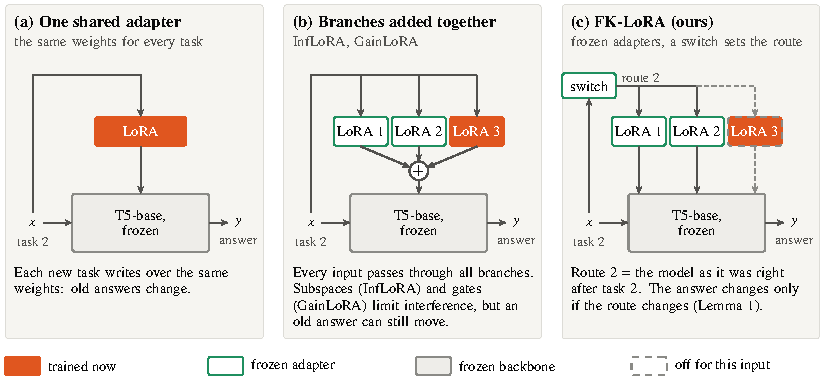
\includegraphics[width=\linewidth]{figures/overview}
  \caption{Three ways to add a task, shown while task~3 is being learned and an input of task~2 is
  answered. (a)~One shared adapter is trained again for each task, so old answers change.
  (b)~InfLoRA and GainLoRA add one branch per task, and every input passes through all branches
  (weighted by gates in GainLoRA); a chosen subspace or the gates limit what a new branch does to
  old inputs, but an old answer can still change. (c)~FK-LoRA never changes an adapter after its
  task has been learned, and a switch sets the route of each input: route~2 is the model as it was
  right after task~2, so the answer changes only if the route changes (Lemma~\ref{lem:route}).}
  \label{fig:overview}
\end{figure}


\subsection{Setting: adapters, routes and answers}
\label{sec:setting}

Let $\mathcal{V}$ be the vocabulary and $E \in \R^{|\mathcal{V}| \times d}$ the input embedding
table of the base model; $E$ and all other base weights $\theta_0$ are frozen. An input is a
sequence of tokens $x = (x_1, \dots, x_L)$. Task $k$ adds a LoRA adapter \citep{hu2022lora} to every adapted weight matrix $W_0$ of the base
model, $\Delta W_k = \tfrac{\alpha}{r} B_k A_k$ with rank $r$. After $T$ tasks an adapted layer
computes
\begin{equation}
  h \;=\; \Bigl( W_0 + \sum_{k=1}^{T} g_k(x)\, \Delta W_k \Bigr) z ,
  \qquad g_k(x) \in \{0, 1\},
  \label{eq:layer}
\end{equation}
where $z$ is the input of the layer and $g_k(x)$ switches adapter $k$ on or off for the whole input
$x$, in every adapted layer. The methods of this paper differ only in the switches. All of
them use a \emph{route} $\rho_T(x) \in \{1, \dots, T\}$ and set
\begin{equation}
  g_k(x) \;=\; \mathbf{1}\bigl[\, k \le \rho_T(x) \,\bigr] ,
  \label{eq:gates}
\end{equation}
so an input with route $j$ is processed with the adapters of tasks $1, \dots, j$,
the model as it was right after task $j$ had been learned. The answer after $T$ tasks is
\begin{equation}
  y_T(x) \;=\; F\bigl(x;\; \theta_0,\; \{A_k, B_k\}_{k \le \rho_T(x)}\bigr),
  \label{eq:answer}
\end{equation}
where $F$ runs the model with a deterministic decoding rule (greedy in all our experiments).

\begin{lemma}[An answer changes only with its route]
\label{lem:route}
Assume that the adapters of a task are never changed after the task has been learned, that the
base model, its tokenizer, the input template and truncation are fixed, and that decoding is
deterministic. Then for every rule that sets the route, every input $x$ and all times $T' > T$:
if $\rho_{T'}(x) = \rho_T(x)$, then $y_{T'}(x) = y_T(x)$.
\end{lemma}

\begin{proof}
Let $j = \rho_T(x) = \rho_{T'}(x)$, so $j \le T$. By Eq.~\eqref{eq:answer} both answers are
$F(x; \theta_0, \{A_k, B_k\}_{k \le j})$. The adapters of the tasks $1, \dots, j$ exist at time $T$
and are the same at time $T'$, and $F$ is deterministic.
\end{proof}

The lemma uses nothing about the model except that it is a deterministic function of its input and
of the adapters that are switched on. It turns retention into a property of the route.

\begin{figure}[t]
  \centering
  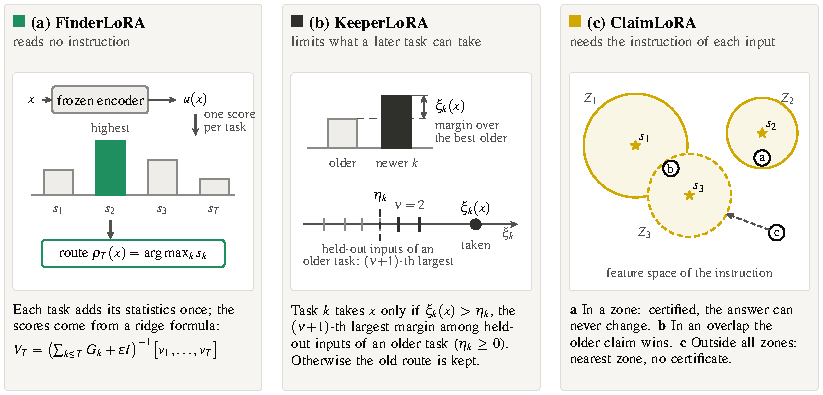
\includegraphics[width=\linewidth]{figures/switch}
  \caption{The three rules that set the route. (a)~\recog{} reads no instruction: it scores every
  task on a frozen feature $u(x)$ of the input with one ridge formula and takes the highest score.
  (b)~\handicap{} adds a handicap for a new task: task $k$ takes an input only if its margin
  $\xi_k(x)$ over the best older task is above $\eta_k$, the $(\nu+1)$-th largest margin among the
  held-out inputs of an older task ($\nu = 2$ in our runs). (c)~\cert{} needs the instruction of
  each input: a task owns a protected zone around the signature of its instruction; an input in a
  zone is certified and belongs to the oldest zone that contains it, and an input outside every
  zone goes to the nearest zone without a certificate.}
  \label{fig:switch}
\end{figure}


% =====================================================================================
\subsection{Without instructions: a recogniser, an audit, and a handicap}
\label{sec:audit}

One classifier over all tasks decides the route from a frozen feature of the whole input, so no
task can be blocked and nothing has to be known about how a task is worded. Its guarantees are
an \emph{audit}, an estimate and a confidence bound from held-out inputs of the share of a task's
answers that have changed, and a \emph{handicap}, a limit known in advance on what a later task
can take from an older one. The audit is ordinary held-out estimation and the handicap a conformal
rank argument with a union bound; what is new is that, by Lemma~\ref{lem:route}, both become
statements about answers.

\paragraph{The price of having no instruction.} For any system whose answer depends on the input alone, two tasks whose inputs overlap
cannot both be answered well: what the older task loses plus what the newer one loses is at least
a conflict $\Omega_{jk}$, the overlap of the two input distributions weighted by how much the best
answers differ (Proposition~\ref{prop:noinstructionprice}). If no input belongs to both tasks,
nothing is forced; this is the exact sense in which an instruction gives the task away. A switch
can only choose how the loss is split: the zones put it on the newer task, \recog{} and
\handicap{} a measured or limited part of it on the older one.

\paragraph{A joint recogniser.} Let $u(x) \in \mathbb{R}^d$ be a frozen feature of the whole
input (the mean of the last-layer states of the frozen encoder of the base
model, without adapter, standardised with the mean and standard deviation of a fixed pool of
instances of other tasks, Section~\ref{sec:protocol}), and
$\bar u(x) = (u(x), 1)$. When task $k$ arrives, its
training inputs are split at random into fit inputs $D_k^{\mathrm{f}}$ and $m$ held-out inputs
$c_1, \dots, c_m$. With $G_k = |D_k^{\mathrm{f}}|^{-1} \sum_{x \in D_k^{\mathrm{f}}} \bar u(x)\, \bar u(x)^{\!\top}$ and $v_k = |D_k^{\mathrm{f}}|^{-1} \sum_{x \in D_k^{\mathrm{f}}} \bar u(x)$ (so every task has the same weight),
the recogniser after $T$ tasks is
\begin{equation}
  V_T \;=\; \Bigl(\, \sum_{k \le T} G_k + \varepsilon\, I \Bigr)^{-1} \bigl[\, v_1, \dots, v_T \,\bigr]
  \label{eq:recogniser}
\end{equation}
with a fixed $\varepsilon > 0$, and the route of an input is the task with the largest score, the older task in a tie,
\begin{equation}
  \rho_T(x) \;=\; \arg\max_{k \le T}\ \bigl(\bar u(x)^{\!\top} V_T\bigr)_k .
  \label{eq:jointroute}
\end{equation}
$V_T$ is the ridge regression of the task labels on the features of all tasks seen so far. The
sums are only added, so it is the same for every order of arrival, no input is kept, and every task
has a column of its own: no task is blocked. The adapter of a task may be trained on all of its
inputs, the held-out ones included; the recogniser never sees those. Such a recogniser is known
from class-incremental learning on frozen features \citep{mcdonnell2023ranpac,zhuang2022acil}; what
we add is what is said about its routes.

\begin{proposition}[An audit of forgetting from held-out inputs]
\label{prop:audit}
Fix a task $j$ and two times $T' > T \ge j$. Let the fit inputs of all tasks and the choice of the
later tasks be independent of the held-out inputs $c_1, \dots, c_m$ of task $j$ and of a further
input $X$ of task $j$, let the route at every time be fitted without them (as in
Eqs.~\eqref{eq:recogniser}--\eqref{eq:jointroute}), and let $c_1, \dots, c_m, X$ be exchangeable
given everything else. Let $H$ be the number of held-out inputs with
$\rho_{T'}(c_i) \ne \rho_T(c_i)$. Then
\[
  \Pr\bigl[\, y_{T'}(X) \ne y_T(X) \,\bigr] \;\le\; \Pr\bigl[\, \rho_{T'}(X) \ne \rho_T(X) \,\bigr]
  \;=\; \mathbb{E}\Bigl[\frac{H}{m}\Bigr] .
\]
If the inputs are independent draws, then with probability at least $1 - \delta$ over the held-out
inputs, the share of the inputs of task $j$ whose route differs between $T$ and $T'$ is at most
the one-sided Clopper--Pearson upper bound for $H$ successes in $m$ trials at confidence
$1 - \delta$. Both statements also hold when ``differs between $T$ and $T'$'' is replaced by ``is
not the same at all times from $T$ to $T'$'', with $H$ counted in the same way.
\end{proposition}

\begin{proof}
The first inequality holds input by input, by Lemma~\ref{lem:route}. Let
$I(x) = \mathbf{1}[\rho_{T'}(x) \ne \rho_T(x)]$. Given everything but $c_1, \dots, c_m, X$ the two
routes are fixed functions, so $I(c_1), \dots, I(c_m), I(X)$ are exchangeable
and $\Pr[I(X) = 1] = \mathbb{E}[I(c_i)] = \mathbb{E}[H]/m$. For independent draws, $H$ is, given
the routes, binomial with $m$ trials and success probability equal to the share in question, and
the second statement is the definition of the Clopper--Pearson bound. The last sentence follows
with $I(x)$ the indicator that the route of $x$ is not constant from $T$ to $T'$.
\end{proof}

So $H/m$ is an unbiased estimate of the share of changed routes, and the confidence bound is the
guarantee. The later tasks may not be chosen by looking at the held-out inputs, nor at anything
computed from them, for example the answers of the adapters of task $j$, which may have been
trained on them. The bound is for one task and one pair of times; for all tasks and all arrivals
the level has to be divided by the number of readings (the ``at all times'' form covers every time in between for one task with a single reading). The audit needs only the features of the
held-out inputs, no pass through the language model, and can be read before the adapter of a new
task is trained: a system knows which older tasks a newcomer disturbs, and by how much, before it
learns the newcomer. It says nothing in advance, and it is not valid for held-out inputs that were
used to decide the routes, as the variant below does.

\paragraph{A handicap for the newcomer.} When task $k \ge 2$ arrives, compute $V_k$ by
Eq.~\eqref{eq:recogniser} and, for any input, the margin of the newcomer over the best older task,
$\xi_k(x) = (\bar u(x)^{\!\top} V_k)_k - \max_{i < k} (\bar u(x)^{\!\top} V_k)_i$. Fix an integer
$\nu \ge 0$. For each older task $j < k$, take the $(\nu+1)$-th largest value of $\xi_k$ among the
held-out inputs of task $j$ ($-\infty$ if task $j$ has at most $\nu$ of them). Let $\eta_k$ be the
largest of these values, or zero if that is larger. The newcomer \emph{takes} an input if
$\xi_k(x) > \eta_k$, and the route is the newest task that took the input:
\begin{equation}
  \rho_T(x) \;=\; \max\bigl\{\, k \le T : \ k = 1 \ \text{ or } \ \xi_k(x) > \eta_k \,\bigr\} .
  \label{eq:handicap}
\end{equation}
$V_k$ and $\eta_k$ are stored when task $k$ arrives and never changed. A newcomer takes an input
only if the joint recogniser prefers it to every older task, and it takes at most $\nu$ of the
held-out inputs of each older task.

\begin{theorem}[A bound in advance without zones]
\label{thm:handicap}
Let the route be set by Eq.~\eqref{eq:handicap}, under the conditions of
Lemma~\ref{lem:route}. Let $X$ be an input of task $j$ that is exchangeable
with the $m$ held-out inputs $c_1, \dots, c_m$ of task $j$ given everything else, and let the
later tasks and their fit inputs be independent of $(c_1, \dots, c_m, X)$, for example fixed in
advance. If the sequence ends with task $T_{\mathrm{end}}$, then
the probability that the answer to $X$ changes at any time after task $j$ has arrived is at most
the probability that its route does, and
\[
  \Pr\bigl[\ \text{there are } j \le T < T' \le T_{\mathrm{end}} \text{ with } \rho_{T'}(X) \ne \rho_T(X) \ \bigr]
  \;\le\; \frac{(T_{\mathrm{end}} - j)\,(\nu+1)}{m+1} .
\]
\end{theorem}

\begin{proof}
By Eq.~\eqref{eq:handicap} the route of an input changes at the arrival of task $k$ only if the
newcomer takes it, that is, only if $\xi_k(X) > \eta_k$, and at no other time, because
the margins and thresholds of the earlier tasks are frozen. The function $\xi_k$ is fitted on fit
inputs only, so given everything else $\xi_k(c_1), \dots, \xi_k(c_m), \xi_k(X)$ are exchangeable. The threshold $\eta_k$ depends on the
held-out inputs, but all that is used is that it is at least the $(\nu+1)$-th largest of the
first $m$ of these numbers. Among $m + 1$ exchangeable numbers, the last one is strictly larger
than the $(\nu+1)$-th largest of the others with probability at most $(\nu+1)/(m+1)$, ties
included. A union bound over the $T_{\mathrm{end}} - j$ later tasks gives the claim.
\end{proof}

\paragraph{Limits.} These statements bound change, not quality: an input that the recogniser gives to the wrong task from the start does not change. The price of the handicap is paid by the newcomer when it arrives, and its bound grows with the number of later tasks and falls with the number of held-out inputs. All statements need test inputs like the training inputs of the task and later tasks not chosen by looking at the held-out inputs; they hold for every wording of an instruction, and when there is none (Remark~\ref{rem:auditlimits}).

\subsection{With instructions: word-vector features of the opening}
\label{sec:features}

When every input carries the instruction of its task, a second rule gives an exact statement instead
of a measured one. Every input of task $k$ is built from a template: the same text, the task's
instruction, then the instance. The part before the instance is the \emph{opening} $o_k$ of the task,
$n_k$ tokens long, found as the longest common token prefix of the template filled with two different
instances (Appendix~\ref{app:impl}). An input that begins with it is in the task's \emph{original
wording}, or \emph{unedited}. The rule of the next four subsections looks at the opening only.

Let $\mathcal{B}$ be a fixed collection of \emph{unrelated} inputs from tasks that are never learned
(Section~\ref{sec:protocol}), and $p(v)$ the share of token $v$ among its tokens. Tokens are weighted
as in \citet{arora2017simple}, so that frequent tokens count little:
\begin{equation}
  w(v) \;=\; \frac{a}{a + p(v)} , \qquad a = 10^{-3}.
  \label{eq:weights}
\end{equation}
The \emph{prefix average} of the first $n$ tokens is
\begin{equation}
  \varphi_n(x) \;=\; \frac{\sum_{i=1}^{\min(n, L)} w(x_i)\, E_{x_i}}{\sum_{i=1}^{\min(n, L)} w(x_i)} \;\in\; \R^d ,
  \label{eq:prefix}
\end{equation}
and $\varphi_\infty(x)$ is the average over the whole input. With $\mu$ and $C$ the mean
and covariance matrix of $\{\varphi_{64}(b) : b \in \mathcal{B}\}$ (64 is a fixed choice of the order of a typical opening), the averages are rescaled by
\begin{equation}
  \hat{C} \;=\; \tfrac{1}{2}\, C + \tfrac{1}{2}\, \frac{\operatorname{tr} C}{d}\, I ,
  \qquad
  \psi_n(x) \;=\; \hat{C}^{-1/2} \bigl( \varphi_n(x) - \mu \bigr) ,
  \label{eq:whiten}
\end{equation}
where the shrinkage towards the identity keeps $\hat{C}$ well conditioned. These quantities depend
only on the base model and on $\mathcal{B}$ and are computed once, before the first task.

\subsection{Protected zones}
\label{sec:zones}

\begin{definition}[Signature, radius, zone]
When task $k$ is learned, it stores three things. Its \emph{signature} is the feature of its opening,
\begin{equation}
  s_k \;=\; \psi_{n_k}(o_k) \;=\; \psi_{n_k}(x) \quad \text{for every input } x \text{ of task } k \text{ in its original wording}.
  \label{eq:signature}
\end{equation}
Let $\mathcal{S}_k$ be the set of signatures known at that moment: those of the unrelated
tasks from which $\mathcal{B}$ is drawn (computed from their openings in the same way) and
$s_1, \dots, s_{k-1}$. The \emph{radius} of task $k$ is
\begin{equation}
  R_k \;=\; \kappa \cdot \min_{s \in \mathcal{S}_k} \lVert s_k - s \rVert_2 , \qquad \kappa = \tfrac{1}{2} .
  \label{eq:radius}
\end{equation}
The \emph{protected zone} of task $k$ and the \emph{relative distance} of an input from task $k$ are
\begin{equation}
  Z_k \;=\; \{\, x \;:\; \lVert \psi_{n_k}(x) - s_k \rVert_2 \le R_k \,\} ,
  \qquad
  \delta_k(x) \;=\; \frac{\lVert \psi_{n_k}(x) - s_k \rVert_2}{R_k} ,
  \label{eq:zone}
\end{equation}
so that $x \in Z_k$ exactly when $\delta_k(x) \le 1$. If $R_k = 0$ (the signature equals a known one), we set $\delta_k(x) = 0$ for inputs at distance zero and
$\delta_k(x) = \infty$ for all others.
\end{definition}

The triple $(n_k, s_k, R_k)$ is all that is kept about task $k$ besides its frozen adapter: no
example, no statistic of hidden activations and no trained module. The zone is a ball around the
signature that reaches half-way to the nearest task known when it was created. Zones can overlap,
because the radius of an older zone was fixed before newer signatures existed and each zone measures
distance in its own feature $\psi_{n_k}$; an input in several zones goes to the oldest. An input
whose first $n_k$ tokens are $o_k$ has $\delta_k(x) = 0$; an input whose instruction was edited
is in $Z_k$ as long as the edit moves the weighted average of its first $n_k$ tokens by at most $R_k$.

\subsection{The certified switch}
\label{sec:switch}

\begin{definition}[Route and certificate]
After $T$ tasks, the \emph{certificate} of an input and its \emph{route} are
\begin{align}
  c_T(x) &\;=\; \mathbf{1}\bigl[\, x \in Z_1 \cup \dots \cup Z_T \,\bigr] , \label{eq:certificate}\\[2pt]
  \rho_T(x) &\;=\;
  \begin{cases}
    \min \{\, k \le T : x \in Z_k \,\} & \text{if } c_T(x) = 1 \quad \text{(the oldest zone that contains } x \text{)}, \\[2pt]
    \arg\min_{k \le T}\; \delta_k(x) & \text{if } c_T(x) = 0 \quad \text{(the nearest zone)} .
  \end{cases}
  \label{eq:route}
\end{align}
\end{definition}

An input inside a zone is \emph{certified}; one outside every zone still gets an answer, from the
task whose zone is nearest in units of its own radius, but without a certificate. Ties between
tasks go to the older one under every rule that uses zones or centres. We call the rule of
Eq.~\eqref{eq:route} \cert{}. A variant of the step for inputs outside every zone, which takes
the scale from the unrelated tasks only, is tested in Section~\ref{sec:paraphrase}. Two simpler
rules serve as comparisons: \nearest{} uses $\arg\min_k \delta_k(x)$ for every input and gives
older zones no priority; \centre{} gives an input to the task whose stored centre (the mean of
$\psi_\infty$ over its training inputs, with the statistics of Eq.~\eqref{eq:whiten} computed from
whole-input averages) is nearest to $\psi_\infty(x)$. This is the fallback of the first version of
our method, but with the token weights of Eq.~\eqref{eq:weights}; the first version weighted all
tokens equally and behaved differently (Appendix~\ref{app:history}).

\paragraph{Learning a task.} (1) Compute $n_t$, $s_t$ and $R_t$ from the task's inputs and store
them; $Z_t$ is fixed from now on. (2) Count and report the training inputs in an older zone,
$b_t = |\{x \in D_t : x \in Z_1 \cup \dots \cup Z_{t-1}\}|$. (3) Add a new adapter $(A_t, B_t)$ with
$B_t = 0$ and freeze all older adapters. (4) Train $(A_t, B_t)$ on the task's data with the usual
loss and nothing added, with the switches of Eq.~\eqref{eq:gates} in place. A training input of
task $t$ has $\delta_t(x) = 0$. If no older zone contains it, its route is $t$, as in plain
sequential training of adapters. Otherwise its route is smaller than $t$, the new adapter is off
on it and it gives no gradient; we call such an input \emph{blocked} and say that task $t$
\emph{collides} with the older task.

\paragraph{Answering.} For an input $x$, compute $\psi_{n}(x)$ for the distinct opening lengths, the
relative distances $\delta_1(x), \dots, \delta_T(x)$, the route and the certificate
(Eqs.~\eqref{eq:certificate}--\eqref{eq:route}), and run the model once with the adapters
$1, \dots, \rho_T(x)$. Return $y_T(x)$ with $c_T(x)$. The extra cost, one embedding lookup, one
product with $\hat C^{-1/2}$ per opening length and $T$ distances, is negligible next to one pass
through the model (Algorithm~\ref{alg:switch}).

\begin{algorithm}
  \caption{The certified switch}
  \label{alg:switch}
  \small
  \begin{tabular}{@{}r@{\hspace{0.8em}}p{0.92\linewidth}@{}}
    \multicolumn{2}{@{}l}{\textbf{Once}, before the first task (frozen embedding table $E$, unrelated inputs $\mathcal{B}$):} \\[1pt]
    1 & compute the token weights $w$ (Eq.~\ref{eq:weights}), the mean $\mu$ and the rescaling $\hat{C}^{-1/2}$ (Eq.~\ref{eq:whiten}), and the
        signatures of the unrelated tasks \\[4pt]
    \multicolumn{2}{@{}l}{\textbf{Learn task $t$} (training inputs $D_t$; zones and adapters of tasks $1, \dots, t-1$):} \\[1pt]
    2 & $o_t \leftarrow$ the opening of task $t$ (the longest common token prefix of its template filled with two instances); \quad $n_t \leftarrow$ its length in tokens \\
    3 & $s_t \leftarrow \psi_{n_t}(o_t)$; \quad $R_t \leftarrow \kappa \cdot \min_{s \in \mathcal{S}_t} \lVert s_t - s \rVert_2$
        \hfill \emph{the zone $Z_t$ is fixed from here on} \\
    4 & $b_t \leftarrow \bigl|\{x \in D_t : x \in Z_1 \cup \dots \cup Z_{t-1}\}\bigr|$; \quad report $b_t$
        \hfill \emph{blocked inputs} \\
    5 & add adapter $t$ with a zero update; freeze the adapters $1, \dots, t-1$ \\
    6 & train adapter $t$ on $D_t$ with the usual loss; each input $x$ is processed with the adapters $1, \dots, \rho_t(x)$ \\[4pt]
    \multicolumn{2}{@{}l}{\textbf{Answer input $x$} (after $T$ tasks):} \\[1pt]
    7 & $\delta_k \leftarrow \lVert \psi_{n_k}(x) - s_k \rVert_2 \,/\, R_k$ \quad for $k = 1, \dots, T$ \quad (with the convention of Definition~1 if $R_k = 0$) \\
    8 & \textbf{if} some $\delta_k \le 1$: \quad $\rho \leftarrow \min\{k : \delta_k \le 1\}$, \quad $c \leftarrow 1$
        \hfill \emph{the oldest claim wins} \\
    9 & \textbf{else}: \quad $\rho \leftarrow \arg\min_k \delta_k$, \quad $c \leftarrow 0$
        \hfill \emph{nearest zone, no certificate} \\
    10 & \textbf{return} the answer of the base model with the adapters $1, \dots, \rho$, together with $c$ \\
  \end{tabular}
\end{algorithm}

\subsection{What the zones guarantee}
\label{sec:guarantee}

\begin{theorem}[Write-once answers]
\label{thm:writeonce}
Assume that zones and adapters are never changed after they have been created, that the base model, its tokenizer, the input template and truncation, and the quantities of Section~\ref{sec:features} are fixed, and that decoding is deterministic. Let
$x$ be any input with $c_T(x) = 1$. Then for every later time $T' \ge T$ and for every choice of the
tasks $T+1, \dots, T'$,
\[
  c_{T'}(x) = 1, \qquad \rho_{T'}(x) = \rho_T(x), \qquad y_{T'}(x) = y_T(x) .
\]
\end{theorem}

\begin{proof}
Let $j = \rho_T(x) = \min\{k \le T : x \in Z_k\}$. The zones $Z_1, \dots, Z_T$ are the same sets at
time $T'$, because the triples $(n_k, s_k, R_k)$ and the feature map are fixed. Hence
$\{k \le T' : x \in Z_k\} = \{k \le T : x \in Z_k\} \cup \{k : T < k \le T',\ x \in Z_k\}$. The first
set is non-empty with minimum $j \le T$, and every element of the second set is larger than $T$, so
the minimum of the union is $j$. Therefore $c_{T'}(x) = 1$ and $\rho_{T'}(x) = j$. By
Eq.~\eqref{eq:answer} the answer depends on $x$, on $\theta_0$ and on the adapters $1, \dots, j$
only; none has changed and decoding is deterministic, so $y_{T'}(x) = y_T(x)$.
\end{proof}

The proof does not use the data of later tasks, their number, their similarity to old tasks or the
way their adapters are trained. Appendix~\ref{app:methoddetails} states and proves the following.
Zero forgetting follows for any set of certified test inputs and any fixed deterministic metric
(Corollary~\ref{cor:zero}); the proof holds for any zone fixed at arrival and decided reproducibly
(Remark~\ref{rem:otherzones}). An input in the original wording is always certified
(Proposition~\ref{prop:own}), and an edit that removes or adds at most a share $R_k/D$ of the token
weight of the opening, with $D$ the largest distance between two rows of the rescaled embedding
table, keeps it certified (Proposition~\ref{prop:edits}); a permutation of the opening is not an
edit for the switch, which reads which words open an input, not their order. The $b_t$ training
inputs of task $t$ that lie in an older zone are routed to the older task for ever and give no
gradient; $b_t$ is known before training, and if it is zero and every training input carries the opening, training is that of plain adapters
(Proposition~\ref{prop:price}). An uncertified input can change its route only to a task nearer to
it than all old ones (Proposition~\ref{prop:uncertified}). The guarantee covers certified inputs
only, gives older tasks priority and rules out backward transfer (Remark~\ref{rem:consequences}).
The limit $\kappa \to 0$ and the rule \keyswitch{}, which matches the opening token for token and
gives all adapters to an input that matches none, are in Remark~\ref{rem:keyswitch}; exactness in
floating point is in Remark~\ref{rem:exactness}.

\subsection{A variant for collections with sibling tasks}
\label{sec:exactfirst}

A new task whose instruction resembles an old one lies inside the old zone, and its inputs are
blocked (Section~\ref{sec:many} measures how often). The rule \exactfirst{} was designed after that
measurement; its guarantee is weaker than Theorem~\ref{thm:writeonce}. It sends an input to the
oldest task whose opening the input carries token for token, if any, and otherwise routes as
\cert{} (Eq.~\eqref{eq:exactfirst}), and it certifies an input that has such an opening or lies in
a zone. The unedited inputs of a new task then go to it even inside an older zone; only a task
whose opening is, or begins with, an older opening still cannot be learned. A sibling is served only
word for word: an edited input of the sibling inside the old zone goes to the old task with a
certificate, and the certificate stands for an unconditional promise for exact claims and a
conditional one for the other inputs in a zone. Proposition~\ref{prop:exactfirst} says that the
route of an exact claim never changes, that another input in a zone keeps its route unless a later
opening is carried by it token for token, and that the rule differs from \cert{} only when an older
zone contains an unedited input of a newer task. On our two benchmark sequences no task lies inside
the zone of another, and \exactfirst{} gives the same route as \cert{} for every test input in
every wording (\ExactSameFive{} and \ExactSameFifteen{} inputs, checked by computation), so every
result for \cert{} on these sequences holds for \exactfirst{} unchanged.

\begin{table}[t]
  \caption{What each rule promises about the route of an input when later tasks are learned.
  ``Unedited'': the input carries the opening of a learned task token for token. ``One exception'':
  a later task whose opening is, token for token, the beginning of that input. Ties between tasks
  with the same opening go to the older task under every rule. $^*$ Unless its opening begins with an older one.}
  \label{tab:guarantees}
  \centering
  \footnotesize
  \setlength{\tabcolsep}{4pt}
  \begin{tabular}{lllll}
    \toprule
    Rule & Unedited input & Edited, inside a zone & Outside every zone & Sibling of an old task \\
    \midrule
    \cert{} & fixed for ever & fixed for ever & may change & blocked and reported \\
    \exactfirst{} & fixed for ever & fixed, with one exception & may change & learned$^*$ \\
    \nearest{} & fixed for ever & may change & may change & learned \\
    \bottomrule
  \end{tabular}
\end{table}

% =====================================================================================
\subsection{Zones from the inputs of a task: a bound that does not grow with later tasks}
\label{sec:bound}

Theorem~\ref{thm:writeonce} does not say how many inputs of a task lie in its zone. For an unedited
instruction it is all of them (Proposition~\ref{prop:own}); for reworded instructions we could only
measure it (Section~\ref{sec:paraphrase}). Without any instruction the share can be guaranteed in
advance: the zone is built from the task's own inputs, with its size set on held-out inputs of the
task. This is the one bound in the paper that needs no instruction and does not grow with the
number of later tasks. In our tests it held, but with the features we tried the zones of early
tasks held inputs of later tasks, which were then blocked (Section~\ref{sec:noinstruction}); the
recogniser of Section~\ref{sec:audit} avoids this.

Split the training inputs of task $k$ into fit inputs and $m$ calibration inputs, take a score
$a_k(x)$ of how unlike the fit inputs an input is (not depending on the calibration inputs), and let
$Z_k$ be the inputs whose score is at most the $\lceil (1-\beta)(m+1)\rceil$-th smallest calibration
score (Eq.~\eqref{eq:inputzone}); the switch is used as before. For an input $X$ exchangeable with the
calibration inputs, the probability that its answer ever changes, whatever the later tasks, is at
most $\Pr[X\notin Z_k]\le\beta$ (Theorem~\ref{thm:bound}), so the expected forgetting of every task
is at most $M\beta$ for a score in $[0,M]$ (Corollary~\ref{cor:bound}). The bound is on change, not
quality; the share of inputs in an older zone is measured, not controlled, and the probability is
over the calibration and test inputs together (Remark~\ref{rem:boundlimits}). For the zones of
Section~\ref{sec:zones} the same holds with $\beta = 0$ for unedited inputs.

\subsection{Compared methods}
\label{sec:compared}

\begin{table}[t]
  \caption{Methods in this study. ``Stored per task'' excludes the frozen adapters; \recog{} also keeps one matrix for all tasks, and \recog{} and \handicap{} keep the features of the held-out inputs of a task. The first two rows read no instruction; \keyswitch{}, \nearest{}, \cert{} and \exactfirst{} read the opening, and \centre{} the whole input. $^\dagger$ Unless a later opening extends theirs.}
  \label{tab:methods}
  \centering
  \footnotesize
  \setlength{\tabcolsep}{3pt}
  \begin{tabular}{llll}
    \toprule
    Method & Which adapters answer an input & Stored per task & Guarantee \\
    \midrule
    \recog   & task with the largest recogniser score & one vector & audit (Prop.~\ref{prop:audit}) \\
    \handicap & newest task that took the input & weights, threshold & Thm.~\ref{thm:handicap} \\
    \midrule
    \plain   & all adapters on for every input & nothing & none \\
    \keyswitch & exact match of the opening; else all on & the opening & unedited inputs$^\dagger$ \\
    \centre  & nearest centre of the whole input & one vector & none \\
    \nearest & nearest zone & signature, radius & unedited inputs \\
    \cert    & oldest zone holding the input; else nearest zone & signature, radius & inputs in a zone \\
    \exactfirst & oldest exact opening; else as \cert{} & also the opening & Prop.~\ref{prop:exactfirst} \\
    InfLoRA  & all on; updates restricted to a subspace & subspace bases & none \\
    GainLoRA & all on, scaled by learned gates & subspace bases, gates & none \\
    \bottomrule
  \end{tabular}
\end{table}

All rules except the last two use the same adapters, trained once; only the switches differ at test
time. No training input was blocked in our GPU runs, so this training was that of \plain{}, the
plain-adapter mode of the code base (one new LoRA per task, older ones frozen, all added, no
penalty; often called IncLoRA). InfLoRA \citep{liang2024inflora} and GainLoRA
\citep{liang2025gainlora} run with their official implementation. InfLoRA restricts the update of
each new adapter to a subspace intended not to interfere with earlier tasks and trains one matrix.
GainLoRA adds to each new branch a gating module that is constrained to stay near zero on inputs of
earlier tasks.

\subsection{Experimental protocol}
\label{sec:protocol}

\paragraph{Code base and setting.} All GPU experiments use the official GainLoRA repository at
commit \texttt{e9d0d70} with its data, trainer and metrics, on the SuperNI benchmark
\citep{wang2022superni}. An input is ``\texttt{Definition:} $\langle$definition$\rangle$
\texttt{Now complete the following example - Input:} $\langle$instance$\rangle$ \texttt{Output:}''.
A launcher sets the switches of Eq.~\eqref{eq:gates} inside the attention modules at run time on top
of the unmodified training script; for the two published methods it only records the test set and
repeats the test with reworded definitions. The published experiments use T5-large and 100 epochs per
task. To fit free GPUs (one or two NVIDIA T4) we use T5-base \citep{raffel2020t5} (220M parameters) and
10 epochs per task; everything else is as in the official scripts: rank $r = 4$, $\alpha = 32$,
learning rate $3 \times 10^{-4}$ with a constant schedule, effective batch size 32, source length 512,
target length 50, greedy decoding, and the checkpoint with the best development Rouge-L.
\textbf{Because of the reduced setting, none of our numbers can be compared with the tables of the
published papers}, and in this setting the two published methods learned less than plain adapters, for
reasons we did not separate (Section~\ref{sec:results}).

\paragraph{Sequences.} (i) Five tasks: relation extraction (\texttt{task1510}), sentiment
of a movie-review sentence (\texttt{task363}, SST-2), cause-event detection (\texttt{task748},
GLUCOSE), tweet sentiment (\texttt{task1687}, Sentiment140) and emotion classification
(\texttt{task875}), each with 800 training and 100 test examples. (ii) The official SuperNI order~1
with 15 tasks, with between 100 and 800 training and between 16 and 100 test examples each.
\textbf{The five tasks were not drawn at random.} In an earlier 15-task run of ours the first three
were the short-input tasks that InfLoRA had forgotten most, and the last two are of the kind after
which that forgetting had happened; the sequence was put together to make forgetting visible.

\paragraph{Unrelated inputs.} The collection $\mathcal{B}$ has 4{,}000 inputs drawn with a
fixed random seed from ten tasks of a different benchmark shipped with the code base (MNLI, CB,
QQP, RTE, DBpedia, AG News, Yahoo, MultiRC, BoolQ and WiC, each with its own definition). None of
these tasks is learned and the zones are never tested on them; the routes of \recog{} are tested
on the whole Long Sequence benchmark (Section~\ref{sec:recogniser}). That benchmark has five more tasks;
its four sentiment tasks were left out on purpose, because the sequences to be learned contain
sentiment tasks, and one task has no definition (Section~\ref{sec:background} looks at how much this
matters).

\paragraph{Reworded definitions.} Each of the five tasks has three reworded definitions: \emph{light}
(a few words changed), \emph{medium} (sentences rewritten) and \emph{heavy} (a different, shorter
formulation). They keep the answer format and are listed in Appendix~\ref{app:rewordings}.
\textbf{They were written by machine during the development of the method, not by people, and the two
design choices of Appendix~\ref{app:history} were made while looking at where these reworded inputs
were routed} (never at an answer of the model). They are a development set, not an independent test;
we call them the development rewordings.

\paragraph{Metrics.} Let $a_{i,j}$ be the Rouge-L score \citep{lin2004rouge} on the test set of task
$j$ after learning task $i$. We report $\mathrm{AP} = \tfrac{1}{T}\sum_{j=1}^{T} a_{T,j}$, the forgetting
$\mathrm{FT} = \tfrac{1}{T-1}\sum_{j=1}^{T-1}\bigl(\max_{j \le i < T} a_{i,j} - a_{T,j}\bigr)$ and
$\mathrm{Learned} = \tfrac{1}{T}\sum_{j} a_{j,j}$, the average score right after learning (the tables
write them in words, with an arrow for the better direction). Learned is shown next to AP and FT
because a low AP can come from forgetting or from learning little. \emph{Answers changed} is the
number of test inputs of the tasks $1, \dots, T-1$ whose answer after the last task differs, as a
string, from the answer right after their own task was learned.

\paragraph{Official test and re-test.} The official code scores each test input against one
reference answer picked at random each time the data are loaded, which adds noise of about one
point for tasks with several references. We therefore report the \emph{official} scores, and a
\emph{re-test}, run after every task with the same weights, that answers every test input with the
original and the reworded definitions and scores it against all references. For methods that share
adapters, an answer depends only on the input and its route, so each pair of an input and a route is
generated once and all rules are evaluated from these answers; differences between rules cannot come
from training noise. The re-test in the original wording reproduces the official answers
(Section~\ref{sec:results}).

\paragraph{Runs without definitions.} The definition of every task is replaced by the empty string in
every data file, for training and testing, so that every input is the same fixed text followed by the instance; nothing else changes. \recog{} and \handicap{} use as
feature the mean of the last-layer states of the frozen T5-base encoder over the tokens of the
instance (at most 256, no adapter), standardised with the mean and standard deviation of 2{,}000
instances drawn at random from the pool of Section~\ref{sec:noinstruction} (real SuperNI tasks outside
the 15 tasks of order~1; not $\mathcal{B}$; for the fourth batch of fresh tasks, the pool instances of
its tasks were left out). Of at most 400 training inputs per task, 200 are held out (half of them for
tasks with fewer than 400) and the rest are fit inputs; test inputs are never used for fitting.
\emph{Fresh tasks} are batches of 30 tasks drawn at random from the collection of
Section~\ref{sec:many}, instances only, with at least 1{,}000 instances each; a batch is used for one
verdict and not again.

\paragraph{Lines fixed before the runs.} For the tests of this paper, what would count as success and
failure was written into the plan of the repository before the run, usually with a guess of the
outcome. The results call a result ``works'', ``does not'' or ``beats'' only as the verdict of such a
line, and say which guesses were wrong and which choices were made after numbers had been seen.

\paragraph{Checks without a GPU.} Where an input is routed depends only on the tokenizer and the
embedding table, so the routes of all test inputs can be computed on a CPU in minutes, for any model.
We use this for the 15-task sequence and several other models (Section~\ref{sec:models}), and report
where such checks were used to make design choices (Appendix~\ref{app:history}).

\section{Results}
\label{sec:results}
Sections~\ref{sec:nodefpublished} to~\ref{sec:nodeftrained} use inputs that carry no instruction; from Section~\ref{sec:five} on, every input carries the definition of its task. Every test was written down in the plan of the repository, with the line by which it would be read, before it was run (Section~\ref{sec:protocol}), except where marked. Unless stated, the setting is reduced: T5-base, 10 epochs per task, one seed (42), re-test scoring, and the five tasks of Section~\ref{sec:five} are among the 15 SuperNI development tasks; a test that says ``routes only'' trains nothing.

\subsection{The published methods without their instructions}
\label{sec:nodefpublished}

\paragraph{The published methods without their instructions.} We repeated the five-task run of Section~\ref{sec:five} for InfLoRA and GainLoRA (official code) with the definition of every task replaced by the empty string, in training and testing, so that every input is the same fixed text followed by the instance. The rows of our own method (plain adapters behind \recog{} of Section~\ref{sec:audit}, tested in Section~\ref{sec:recogniser}) are explained in Section~\ref{sec:nodeftrained}.
Line fixed before the run, for each method against its own run with definitions: if the score right after learning is below 60\% of the score with definitions, the method ``could not learn these tasks''; if it learned, it ``holds its answers less well'' when forgetting rises by at least 5 points, or when the changed answers are at least twice as many and at least 60 of 400 higher. Verdict: both learned (score right after learning far above 60\% of that with definitions) and both hold their answers less well: changed answers rise from \AudPubInfloraDefChanged{} to \AudPubInfloraNoDefChanged{} for InfLoRA and from \AudPubGainloraDefChanged{} to \AudPubGainloraNoDefChanged{} for GainLoRA, of \AudPubCompared{} (Table~\ref{tab:noinstpublished}; per task in Table~\ref{tab:noinstpertask}, Appendix~\ref{app:noinstmore}).
The line was set against the three-seed runs with definitions of Section~\ref{sec:five}; the table gives the same seed. Our guess for GainLoRA was 60 to 150 changed answers: \AudPubGainloraNoDefChanged{}.
Caveats written before the run: one seed, five tasks, a small model, a tenth of the published number of epochs; only these two methods were run, a first look in a reduced setting that says nothing about other methods. The two other seeds read the same (Table~\ref{tab:noinstseeds}): over three seeds, changed answers and forgetting stay far above those with definitions (\FiveInfChanged{} and \FiveGainChanged{} answers, \FiveInfFT{} and \FiveGainFT{} points; Section~\ref{sec:five}).

\begin{table}[t]
  \caption{The five tasks of Section~\ref{sec:five}, with the definition of every task in its inputs or none. Score right after learning, final score (Rouge-L) and forgetting; answers changed: of the \AudPubCompared{} test inputs of the first four tasks, those whose answer at the end differs from the answer right after their task was learned (the last task cannot be forgotten). Rows of ours: plain adapters never blocked, with the routes of Section~\ref{sec:audit}, run without definitions only. Last row: every input sent to its own task.}
  \label{tab:noinstpublished}
  \centering
  {\footnotesize\setlength{\tabcolsep}{3pt}\begin{tabular}{p{1.9in}lrrrr}
    \toprule
    Method & Definitions & \shortstack[r]{Score right\\after\\learning $\uparrow$} & \shortstack[r]{Final\\score $\uparrow$} & \shortstack[r]{Forgetting\\(points) $\downarrow$} & \shortstack[r]{Answers\\changed\\of \AudPubCompared{} $\downarrow$} \\
    \midrule
    InfLoRA & with & \AudPubInfloraDefLearned{} & \AudPubInfloraDefAP{} & \AudPubInfloraDefFT{} & \AudPubInfloraDefChanged{} \\
    InfLoRA & none & \AudPubInfloraNoDefLearned{} & \AudPubInfloraNoDefAP{} & \AudPubInfloraNoDefFT{} & \AudPubInfloraNoDefChanged{} \\
    GainLoRA & with & \AudPubGainloraDefLearned{} & \AudPubGainloraDefAP{} & \AudPubGainloraDefFT{} & \AudPubGainloraDefChanged{} \\
    GainLoRA & none & \AudPubGainloraNoDefLearned{} & \AudPubGainloraNoDefAP{} & \AudPubGainloraNoDefFT{} & \AudPubGainloraNoDefChanged{} \\
    \midrule
    \plain{} (all adapters on) & none & \AudOursAllLearned{} & \AudOursAllAP{} & \AudOursAllFT{} & \AudOursAllChanged{} \\
    \recog{} (ours) & none & \AudOursRidgeLearned{} & \AudOursRidgeAP{} & \AudOursRidgeFT{} & \AudOursRidgeChanged{} \\
    \handicap{}, $\nu = 2$ (ours) & none & \AudOursHandicapLearned{} & \AudOursHandicapAP{} & \AudOursHandicapFT{} & \AudOursHandicapChanged{} \\
    every input to its own task (ceiling) & none & \AudOursOwnLearned{} & \AudOursOwnAP{} & \AudOursOwnFT{} & \AudOursOwnChanged{} \\
    \bottomrule
\end{tabular}}

\end{table}

Table~\ref{tab:conflictcount} counts inputs that occur word for word in two tasks, which Proposition~\ref{prop:noinstructionprice} needs. On both standard benchmarks there are none (\AudConfOneShared{} of \AudConfOneInputs{} for the 15 SuperNI tasks, \AudConfTwoShared{} of \AudConfTwoInputs{} for the 15 Long Sequence tasks). The count is a lower limit of the conflict, since tasks can overlap without sharing a text, so alone it shows only that no loss is forced by shared texts. That the loss of the two methods was not forced is shown by the recogniser of Section~\ref{sec:recogniser}, which gives all but \AudRouteFiveRidgeNotOwn{} of the \AudRouteFiveRidgeN{} test inputs of these five tasks to their own task.

\begin{table}[t]
  \caption{Inputs that occur word for word in two or more tasks of a collection (benchmark training and test inputs; instances read from the task files for the fresh batches of Section~\ref{sec:recogniser}). ``Also elsewhere'': inputs that occur in another task of the collection; \%: their share. A count, not a test.}
  \label{tab:conflictcount}
  \centering
  {\footnotesize\setlength{\tabcolsep}{3pt}\begin{tabular}{lrrrr}
    \toprule
    Collection & Tasks & Inputs & \shortstack[r]{Occur also\\in another\\task} & \shortstack[r]{Share,\\\%} \\
    \midrule
    SuperNI, 15 tasks & \AudConfOneTasks{} & \AudConfOneInputs{} & \AudConfOneShared{} & \AudConfOneShare{} \\
    Long Sequence, 15 tasks & \AudConfTwoTasks{} & \AudConfTwoInputs{} & \AudConfTwoShared{} & \AudConfTwoShare{} \\
    fresh batch 1 & \AudConfThreeTasks{} & \AudConfThreeInputs{} & \AudConfThreeShared{} & \AudConfThreeShare{} \\
    fresh batch 2 & \AudConfFourTasks{} & \AudConfFourInputs{} & \AudConfFourShared{} & \AudConfFourShare{} \\
    fresh batch 3 & \AudConfFiveTasks{} & \AudConfFiveInputs{} & \AudConfFiveShared{} & \AudConfFiveShare{} \\
    \bottomrule
\end{tabular}}

\end{table}

\subsection{Recognising the task without an instruction}
\label{sec:recogniser}

\recog{} and its variant \handicap{} (Section~\ref{sec:audit}) read no instruction and block no task. The zone rule of Section~\ref{sec:bound}, tested first in Section~\ref{sec:noinstruction}, left a better frozen feature as the open question. The corrected form of \handicap{} and its setting were chosen after numbers had been seen, and are marked.

\paragraph{The feature.} The zone rule of Section~\ref{sec:noinstruction} (ratio score, level 0.05, the oldest zone wins) was run with a third frozen feature: the mean of the last-layer states of the frozen T5-base encoder, without adapter, over the tokens of the instance. Development data: the 15 SuperNI tasks of order 1, at most 400 training inputs per task, official test inputs.
Line fixed before the run: ``works'' if on average at least 90\% of the test inputs reach their own task and at most 10\% are blocked. Verdict: ``partial'' (Table~\ref{tab:recogniserfeatures}, top): \AudZoneFrozenTOwn{}\% to the own task and \AudZoneFrozenTBlocked{}\% blocked, far better than the sentence encoder and the word vectors, with changed routes within the claim.
The guess, 20 to 35\% blocked, was wrong in the good direction. A likely reason: a sentence encoder keeps what a text is about and discards how it is written, and the way an input is written is most of what separates tasks. The middle of the table shows it for a joint recogniser on sentence-encoder features: 16 numbers describing the shape of the text (length, capitals, digits, punctuation, line breaks, @, \# and web addresses) raise the share at the own task at the end from \AudRecLrMiniEndSuperni{}\% to \AudRecLrShapeEndSuperni{}\% on SuperNI and also on Long Sequence; character n-grams do about as well as the shape numbers.

\begin{table}[t]
  \caption{Features, development data (the benchmark tasks were used to choose among the variants); means over tasks, in \%. Top: the zone rule with three frozen features on the 15 SuperNI tasks (inside own zone; blocked when the task arrives; own task at the end; route changed). Middle: a joint recogniser fitted by logistic regression or by Eq.~\eqref{eq:recogniser} on random cosine features, on the sentence encoder with or without the shape numbers or character n-grams, for SuperNI and Long Sequence; the last pair of columns is $(H{+}1)/(m{+}1)$, where $H$ of the $m$ held-out inputs of a task changed route (Proposition~\ref{prop:audit}), from the held-out inputs. Bottom: the audit of Proposition~\ref{prop:audit} for the chosen variant (logistic regression with shape numbers): $H/m$ and the 95\% bound.}
  \label{tab:recogniserfeatures}
  \centering
  {\footnotesize\setlength{\tabcolsep}{3pt}\begin{tabular}{lrrrr}
    \toprule
    Feature & \shortstack[r]{Inside own\\zone, \%} & \shortstack[r]{Blocked,\\\% $\downarrow$} & \shortstack[r]{Sent to\\own task\\at the end,\\\% $\uparrow$} & \shortstack[r]{Route\\changed,\\\% $\downarrow$} \\
    \midrule
    word vectors & \AudZoneWordVecInside{} & \AudZoneWordVecBlocked{} & \AudZoneWordVecOwn{} & \AudZoneWordVecChanged{} \\
    sentence encoder & \AudZoneSentenceInside{} & \AudZoneSentenceBlocked{} & \AudZoneSentenceOwn{} & \AudZoneSentenceChanged{} \\
    frozen T5-base states & \AudZoneFrozenTInside{} & \AudZoneFrozenTBlocked{} & \AudZoneFrozenTOwn{} & \AudZoneFrozenTChanged{} \\
    \bottomrule
\end{tabular}}
\par\medskip
{\footnotesize\setlength{\tabcolsep}{1.8pt}\begin{tabular}{lrrrrrr}
    \toprule
    & \multicolumn{2}{c}{\shortstack{Sent to own task\\at the end, \% $\uparrow$}} & \multicolumn{2}{c}{\shortstack{Route changed,\\\% $\downarrow$}} & \multicolumn{2}{c}{\shortstack{Audit\\$(H{+}1)/(m{+}1)$, \%}} \\
    \cmidrule(lr){2-3}\cmidrule(lr){4-5}\cmidrule(l){6-7}
    Recogniser, feature & SuperNI & Long & SuperNI & Long & SuperNI & Long \\
    \midrule
    logistic reg., sentence enc., $C=$\AudRecLrMiniParam{} & \AudRecLrMiniEndSuperni{} & \AudRecLrMiniEndLong{} & \AudRecLrMiniChangedSuperni{} & \AudRecLrMiniChangedLong{} & \AudRecLrMiniAuditLineSuperni{} & \AudRecLrMiniAuditLineLong{} \\
    \textbf{\quad + shape numbers, $C=$\AudRecLrShapeParam{}} & \textbf{\AudRecLrShapeEndSuperni{}} & \textbf{\AudRecLrShapeEndLong{}} & \textbf{\AudRecLrShapeChangedSuperni{}} & \textbf{\AudRecLrShapeChangedLong{}} & \textbf{\AudRecLrShapeAuditLineSuperni{}} & \textbf{\AudRecLrShapeAuditLineLong{}} \\
    \quad + character n-grams, $C=$\AudRecLrCharParam{} & \AudRecLrCharEndSuperni{} & \AudRecLrCharEndLong{} & \AudRecLrCharChangedSuperni{} & \AudRecLrCharChangedLong{} & \AudRecLrCharAuditLineSuperni{} & \AudRecLrCharAuditLineLong{} \\
    cosine features, sentence enc., $\lambda=$\AudRecCosMiniParam{} & \AudRecCosMiniEndSuperni{} & \AudRecCosMiniEndLong{} & \AudRecCosMiniChangedSuperni{} & \AudRecCosMiniChangedLong{} & \AudRecCosMiniAuditLineSuperni{} & \AudRecCosMiniAuditLineLong{} \\
    \quad + shape numbers, $\lambda=$\AudRecCosShapeParam{} & \AudRecCosShapeEndSuperni{} & \AudRecCosShapeEndLong{} & \AudRecCosShapeChangedSuperni{} & \AudRecCosShapeChangedLong{} & \AudRecCosShapeAuditLineSuperni{} & \AudRecCosShapeAuditLineLong{} \\
    \bottomrule
\end{tabular}}
\par\medskip
{\footnotesize\setlength{\tabcolsep}{3pt}\begin{tabular}{lrrrr}
    \toprule
    & \multicolumn{2}{c}{Audit $H/m$, \%} & \multicolumn{2}{c}{95\% bound, \%} \\
    \cmidrule(lr){2-3}\cmidrule(l){4-5}
    Chosen variant & SuperNI & Long & SuperNI & Long \\
    \midrule
    logistic reg. + shape numbers, $C=$\AudRecLrShapeParam{} & \AudRecChosenAuditEstSuperni{} & \AudRecChosenAuditEstLong{} & \AudRecChosenAuditBoundSuperni{} & \AudRecChosenAuditBoundLong{} \\
    \bottomrule
\end{tabular}}

\end{table}

\paragraph{Rules that block nothing.} Development data: the 15 SuperNI tasks, at most 400 training inputs per task, 200 of them held out (half for tasks with fewer than 400), official test inputs; the rules run on the frozen T5-base states, standardised with the statistics of 2{,}000 instances of other SuperNI tasks (the pool of Section~\ref{sec:protocol}, not $\mathcal{B}$).
Rule written before the run: among the variants with at most 3\% changed routes, take the highest share of test inputs at their own task after the last task; ties go to the ridge form, which stores no input. Verdict: it chose \recog{} with the smallest of three penalties (``ridge $1\times$'': in the code a penalty equal to the feature dimension, 768, on sums with total weight 200 per task; in Eq.~\eqref{eq:recogniser}, $\varepsilon = 768/200 = 3.84$), tied with the logistic regression (Table~\ref{tab:recogniserdev}).
It gives \AudDevLLamOneEnd{}\% of the test inputs to their own task after the last task, with \AudDevLLamOneChanged{}\% of the routes changed; the audit of Proposition~\ref{prop:audit} has a 95\% bound of \AudDevLLamOneAuditBound{}\%. The weights are the same for every order of arrival, up to rounding (checked with the order reversed); on the second official order and on five random orders the changed routes run from \AudOrdRandTwoLChanged{}\% to \AudOrdTwoLChanged{}\% (Table~\ref{tab:recogniserorders}, Appendix~\ref{app:noinstmore}).
The guess, 95 to 99\%, held; the guess of 1 to 3\% changed routes was too high (\AudDevLLamOneChanged{}\%). Weak tasks: the tweet task (sentiment140) falls from \AudPtFourteenArrive{}\% to \AudPtFourteenEnd{}\% when the emotion task arrives (\AudPtFourteenC{} of its \AudPtFourteenM{} held-out inputs change route, and the audit shows it) and the dialogue task (multi-woz) ends at \AudPtSevenEnd{}\%; all others end at 99 to 100\% (Table~\ref{tab:recogniserpertask}, Appendix~\ref{app:noinstmore}).

\begin{table}[t]
  \caption{Rules that block nothing, development data: the 15 SuperNI tasks of order 1, frozen T5-base states, means over tasks, in \%. Own task at arrival and after the last task; route changed after the task arrived; audit $H/m$ and 95\% bound (Proposition~\ref{prop:audit}, held-out inputs); bound in advance (Theorem~\ref{thm:handicap} for \handicap{}; for the zone rule the line of the zone paragraph, not a theorem). $C$: inverse penalty of the logistic regression; ridge $1\times$, $10\times$, $100\times$: penalty of Eq.~\eqref{eq:recogniser} in multiples of the smallest; $r$: a new zone may hold at most $r-1$ held-out inputs of an older task. Bold: the variants used later. The last three rows are the first form of \handicap{}, without the floor at zero in Eq.~\eqref{eq:handicap}. The rows were compared on these tasks: development numbers.}
  \label{tab:recogniserdev}
  \centering
  {\scriptsize\setlength{\tabcolsep}{2.5pt}\begin{tabular}{p{1.6in}rrrrrr}
    \toprule
    Rule & \shortstack[r]{Sent to\\own task\\at arrival,\\\% $\uparrow$} & \shortstack[r]{Sent to\\own task\\at the end,\\\% $\uparrow$} & \shortstack[r]{Route\\changed,\\\% $\downarrow$} & \shortstack[r]{Audit\\$H/m$, \%} & \shortstack[r]{95\% bound,\\\%} & \shortstack[r]{Bound in\\advance, \%} \\
    \midrule
    \recog{} with logistic regression ($C = 1$) & \AudDevJCOneArrive{} & \AudDevJCOneEnd{} & \AudDevJCOneChanged{} & \AudDevJCOneAuditEst{} & \AudDevJCOneAuditBound{} & -- \\
    \textbf{\recog{}, ridge $1\times$} & \textbf{\AudDevLLamOneArrive{}} & \textbf{\AudDevLLamOneEnd{}} & \textbf{\AudDevLLamOneChanged{}} & \textbf{\AudDevLLamOneAuditEst{}} & \textbf{\AudDevLLamOneAuditBound{}} & \textbf{--} \\
    \recog{}, ridge $10\times$ & \AudDevLLamTenArrive{} & \AudDevLLamTenEnd{} & \AudDevLLamTenChanged{} & \AudDevLLamTenAuditEst{} & \AudDevLLamTenAuditBound{} & -- \\
    \recog{}, ridge $100\times$ & \AudDevLLamHundredArrive{} & \AudDevLLamHundredEnd{} & \AudDevLLamHundredChanged{} & \AudDevLLamHundredAuditEst{} & \AudDevLLamHundredAuditBound{} & -- \\
    zones, newest wins, $r = 1$ & \AudDevClaimsROneArrive{} & \AudDevClaimsROneEnd{} & \AudDevClaimsROneChanged{} & -- & -- & \AudDevClaimsROneBound{} \\
    \handicap{}, $\nu = 0$ & \AudDevHPrimeTZeroArrive{} & \AudDevHPrimeTZeroEnd{} & \AudDevHPrimeTZeroChanged{} & -- & -- & \AudDevHPrimeTZeroBound{} \\
    \handicap{}, $\nu = 1$ & \AudDevHPrimeTOneArrive{} & \AudDevHPrimeTOneEnd{} & \AudDevHPrimeTOneChanged{} & -- & -- & \AudDevHPrimeTOneBound{} \\
    \textbf{\handicap{}, $\nu = 2$} & \textbf{\AudDevHPrimeTTwoArrive{}} & \textbf{\AudDevHPrimeTTwoEnd{}} & \textbf{\AudDevHPrimeTTwoChanged{}} & \textbf{--} & \textbf{--} & \textbf{\AudDevHPrimeTTwoBound{}} \\
    \handicap{}, $\nu = 5$ & \AudDevHPrimeTFiveArrive{} & \AudDevHPrimeTFiveEnd{} & \AudDevHPrimeTFiveChanged{} & -- & -- & \AudDevHPrimeTFiveBound{} \\
    \handicap{} without protection ($\nu = \infty$) & \AudDevHPrimeTNoneArrive{} & \AudDevHPrimeTNoneEnd{} & \AudDevHPrimeTNoneChanged{} & -- & -- & -- \\
    \midrule
    \handicap{} without the floor (first form), $\nu = 0$ & \AudDevHTZeroArrive{} & \AudDevHTZeroEnd{} & \AudDevHTZeroChanged{} & -- & -- & \AudDevHTZeroBound{} \\
    \handicap{} without the floor (first form), $\nu = 1$ & \AudDevHTOneArrive{} & \AudDevHTOneEnd{} & \AudDevHTOneChanged{} & -- & -- & \AudDevHTOneBound{} \\
    \handicap{} without the floor (first form), $\nu = 2$ & \AudDevHTTwoArrive{} & \AudDevHTTwoEnd{} & \AudDevHTTwoChanged{} & -- & -- & \AudDevHTTwoBound{} \\
    \bottomrule
\end{tabular}}

\end{table}

\paragraph{\handicap{}, and a flaw in its first form.} \handicap{} (Eq.~\eqref{eq:handicap}) puts a bound known in advance on the same joint recogniser. As first written, the threshold $\eta_k$ had no floor at zero: when no held-out input of an older task lies near the newcomer, it is negative and the newcomer takes inputs that even the joint recogniser gives to an older task. For $\nu = 2$ the first form changed more routes than no protection: \AudDevHTTwoChanged{}\% against \AudDevHPrimeTNoneChanged{}\% (also for $\nu = 1$). The guess for $\nu = 0$, 97 to 99\% at the own task, was wrong: \AudDevHTZeroEnd{}\%.
The floor at zero is the correction. It was made after seeing these numbers, on the same 15 tasks, so the numbers of the corrected rule are development numbers; the proof is unchanged. With the floor, the share at the own task at the end is \AudDevHPrimeTZeroEnd{}\% for $\nu = 0$ and \AudDevHPrimeTTwoEnd{}\% for $\nu = 2$, close to no protection, and the changed routes fall to \AudDevHPrimeTTwoChanged{}\% (Table~\ref{tab:recogniserdev}).
We then chose $\nu = 2$, the smallest value within 0.2 points of the best at the end ($\nu = 5$: \AudDevHPrimeTFiveEnd{}\%). With $\nu = 0$ quoref takes only about a third of its own inputs, because one held-out input of the news task sets the threshold (Remark~\ref{rem:auditlimits}(ii)). For $\nu = 2$ the bound in advance averages \AudDevHPrimeTTwoBound{}\%, far above what was measured: it is loose, because most later tasks take nothing from most older ones, which it cannot know.

\paragraph{Zones can do it too, with the right feature.} Four zone shapes were compared on the sentence encoder, before the joint recogniser was chosen, under one rule: the newest zone wins, and no held-out input of an older task may lie inside a new zone, so no task is blocked (15 SuperNI tasks, development data; the Long Sequence part of the grid was not computed).
The rule written before the grid chose one boundary per older task with the shape numbers (weight \AudShapePairShapeWeight{}): \AudShapePairShapeEnd{}\% at the end, \AudShapePairShapeChanged{}\% of the routes changed, against a line of \AudShapePairShapeBound{}\%. The line is the share of a task's test inputs outside its own zone at arrival plus $r/(m+1)$ for every later task; it follows from the rank argument of Theorem~\ref{thm:handicap}, but is used as a line fixed in advance, not stated as a theorem.
The shape matters less than the feature: with the shape numbers three shapes reach \AudShapeOvrShapeEnd{}\% to \AudShapePairShapeEnd{}\%, the balls \AudShapePairKnnShapeEnd{}\%, and without the numbers the same three are lower (Table~\ref{tab:shapesgrid}). No guess was written for the shapes.

\begin{table}[t]
  \caption{Four zone shapes, development data: the 15 SuperNI tasks, sentence encoder alone or with the 16 shape numbers (best weight tried). Rows: one flat boundary against everything older, one per older task, balls, boundaries curved by random cosine features. Means over tasks, in \%: own task after the last task; route changed. Bold: the variant chosen by the rule written before the grid.}
  \label{tab:shapesgrid}
  \centering
  {\footnotesize\setlength{\tabcolsep}{3pt}\begin{tabular}{lrrrrr}
    \toprule
    & \multicolumn{2}{c}{Sentence encoder} & \multicolumn{3}{c}{+ shape numbers} \\
    \cmidrule(lr){2-3}\cmidrule(l){4-6}
    Boundary & \shortstack[r]{Sent to\\own task\\at the end,\\\% $\uparrow$} & \shortstack[r]{Route\\changed,\\\% $\downarrow$} & \shortstack[r]{Sent to\\own task\\at the end,\\\% $\uparrow$} & \shortstack[r]{Route\\changed,\\\% $\downarrow$} & weight \\
    \midrule
    one boundary against everything & \AudShapeOvrMiniEnd{} & \AudShapeOvrMiniChanged{} & \AudShapeOvrShapeEnd{} & \AudShapeOvrShapeChanged{} & \AudShapeOvrShapeWeight{} \\
    one boundary per older task & \AudShapePairMiniEnd{} & \AudShapePairMiniChanged{} & \textbf{\AudShapePairShapeEnd{}} & \textbf{\AudShapePairShapeChanged{}} & \textbf{\AudShapePairShapeWeight{}} \\
    balls around the task's inputs & \AudShapePairKnnMiniEnd{} & \AudShapePairKnnMiniChanged{} & \AudShapePairKnnShapeEnd{} & \AudShapePairKnnShapeChanged{} & \AudShapePairKnnShapeWeight{} \\
    curved boundaries & \AudShapePairRffMiniEnd{} & \AudShapePairRffMiniChanged{} & \AudShapePairRffShapeEnd{} & \AudShapePairRffShapeChanged{} & \AudShapePairRffShapeWeight{} \\
    \bottomrule
\end{tabular}}

\end{table}

\paragraph{Fresh tasks.} Each rule was chosen on the 15 benchmark tasks and read once on a batch of 30 fresh tasks that no earlier test had used (drawn at random from a collection of real tasks, instances only; at least 1{,}000 instances each, the last 200 as test inputs, training and held-out inputs from a random part of the first 800).
Lines fixed before: a rule ``works'' if on average at least 85\% of the test inputs go to their own task, both at arrival and after the last task, ``does not'' below 70\%, else ``partial''; for the oldest-zone-wins rule also at most 15\% blocked, ``does not'' above 30\%; a guarantee is ``met'' if the average changed share is at most the average bound (for the audit, the average $(H{+}1)/(m{+}1)$) plus two standard errors.
Verdicts (Table~\ref{tab:recogniserfresh}): first batch, both zone rules on the sentence encoder did not work (oldest zone wins: \AudShapeFreshFirstOldestEnd{}\% at the end with \AudShapeFreshFirstOldestBlocked{}\% blocked, ``\AudShapeFreshFirstOldestUse{}''; newest zone wins: \AudShapeFreshFirstNewestEnd{}\%, ``\AudShapeFreshFirstNewestUse{}''). Second batch, zone rule with one boundary per older task and shape numbers: \AudShapeFreshSecondEnd{}\% at the end, changed routes within its line of \AudShapeFreshSecondBound{}\%, ``\AudShapeFreshSecondUse{}'', guarantee ``\AudShapeFreshSecondGuarantee{}''. Third batch, joint recogniser (logistic regression, sentence encoder, shape numbers): \AudFreshThirdEnd{}\% at the end, ``\AudFreshThirdUse{}'', audit line $(H{+}1)/(m{+}1)$ \AudFreshThirdAuditLine{}\%, audit ``\AudFreshThirdCert{}''. Fourth batch, \recog{} on the frozen model's states, the rule used for trained answers: \AudFreshFourthLEnd{}\% at the end, ``\AudFreshFourthUse{}'', audit line \AudFreshFourthLAuditLine{}\%, audit ``\AudFreshFourthCert{}''; the changed routes and audit bounds are in the table. The guess, 80 to 90\%, was too low.
On the fourth batch \handicap{} ($\nu = 2$), reported by a line fixed before (within 2 points of \recog{} at the end), reaches \AudFreshFourthHEnd{}\% and changes fewer routes. The batches differ, so the rows do not compare the rules.

\begin{table}[t]
  \caption{Fresh tasks: each rule read once on a batch of 30 tasks that nothing had used. Means over the 30 tasks, in \%: own task at arrival and after the last task; routes changed; audit $H/m$ and 95\% bound where the rule has an audit. Verdict: use / guarantee by the lines in the text. Last column: number of tasks below 70\% own task.}
  \label{tab:recogniserfresh}
  \centering
  {\scriptsize\setlength{\tabcolsep}{2pt}\begin{tabular}{p{0.95in}rrrrrcr}
    \toprule
    Fresh tasks & \shortstack[r]{Sent to\\own task\\at arrival,\\\% $\uparrow$} & \shortstack[r]{Sent to\\own task\\at the end,\\\% $\uparrow$} & \shortstack[r]{Route\\changed,\\\% $\downarrow$} & \shortstack[r]{Audit\\$H/m$, \%} & \shortstack[r]{95\% bound,\\\%} & Verdict & \shortstack[r]{Tasks below\\70\% $\downarrow$} \\
    \midrule
    first batch: zones, oldest wins, sentence encoder & -- & \AudShapeFreshFirstOldestEnd{} & \AudShapeFreshFirstOldestChanged{} & -- & -- & \AudShapeFreshFirstOldestUse{} / \AudShapeFreshFirstOldestClaim{} & -- \\
    first batch: zones, newest wins, sentence encoder & \AudShapeFreshFirstNewestArrive{} & \AudShapeFreshFirstNewestEnd{} & \AudShapeFreshFirstNewestChanged{} & -- & -- & \AudShapeFreshFirstNewestUse{} / \AudShapeFreshFirstNewestGuarantee{} & -- \\
    second batch: zones, newest wins, one boundary per older task, sentence encoder + shape numbers & \AudShapeFreshSecondArrive{} & \AudShapeFreshSecondEnd{} & \AudShapeFreshSecondChanged{} & -- & -- & \AudShapeFreshSecondUse{} / \AudShapeFreshSecondGuarantee{} & -- \\
    third batch: sentence enc. + shape numbers, logistic reg. & \AudFreshThirdArrive{} & \AudFreshThirdEnd{} & \AudFreshThirdChanged{} & \AudFreshThirdAuditEst{} & \AudFreshThirdAuditBound{} & \AudFreshThirdUse{} / \AudFreshThirdCert{} & \AudFreshThirdLow{} \\
    fourth batch: frozen T5-base states, \recog{} & \AudFreshFourthLArrive{} & \AudFreshFourthLEnd{} & \AudFreshFourthLChanged{} & \AudFreshFourthAuditEst{} & \AudFreshFourthAuditBound{} & \AudFreshFourthUse{} / \AudFreshFourthCert{} & \AudFreshFourthLow{} \\
    fourth batch: frozen T5-base states, \handicap{}, $\nu = 2$ & \AudFreshFourthHArrive{} & \AudFreshFourthHEnd{} & \AudFreshFourthHChanged{} & -- & -- & -- & -- \\
    \bottomrule
\end{tabular}}

\end{table}

The failure belongs to the third batch and returns in the fourth. Two tasks of the third batch are built on the same dataset (answers for a question, and a question for an answer); Table~\ref{tab:conflictcount} shows \AudConfFiveShared{} inputs of \AudConfFiveInputs{} (\AudConfFiveShare{}\%) that occur in two tasks, all in this pair, and none in the first two batches (the fourth was not counted). Each of the two gets about half of its own inputs (\AudFreshThirdPairLow{}\% and \AudFreshThirdPairHigh{}\%). This is the conflict of Proposition~\ref{prop:noinstructionprice} in data: \AudConfPairShare{}\% of the inputs of each occur in the other, and on those no method without instructions can do better than split them. The rest of the loss is not forced by this count, though their other inputs are texts of the same kind; the other tasks of the batch are unaffected.
The fourth batch has a pair on the same reading passages (its shared texts were not counted): under \recog{} the older task falls to about half of its inputs when the newer one arrives, and its audit shows it; under \handicap{} the older keeps its routes and the newer is kept out. The price moves; it does not go away.
Caveat from the independent check: the test inputs are the last 200 instances of a task file and the held-out inputs a random part of the first 800. If a file is ordered the two are not the same kind of draw, so the statements about change rest on an assumption not ensured by construction; the shares at the own task do not depend on it.

\paragraph{The second benchmark, and many tasks.} Frozen states were computed on a GPU (they are slow on a CPU); routes only. These tasks had been used to compare features for an earlier variant; \recog{} and its one setting had been fixed on SuperNI before it was read on them.
Line fixed before the run: \recog{} ``works on the second benchmark'' if at least 90\% of all official test inputs of the 15 Long Sequence tasks go to their own task after the last task, ``does not'' below 75\%. Verdict: ``works'', audit ``met'': \AudScaleLongThreeEnd{}\% for both official orders (Table~\ref{tab:recogniserscale}). The guess, 94 to 98\%, held. The weak tasks are two of three entailment tasks: mnli falls to \AudScaleLongMnliEnd{}\% when rte arrives (\AudScaleLongMnliC{} of \AudScaleLongMnliM{} held-out inputs change route) and rte gets \AudScaleLongRteEnd{}\%; under \handicap{} mnli keeps its inputs and rte takes only \AudScaleLongRteHEnd{}\% (Table~\ref{tab:recogniserlongpertask}, Appendix~\ref{app:noinstmore}).
Many tasks, on the three fresh batches that earlier tests had used, so a description and not a verdict: with 30, 60, 90 fresh tasks and all 120 tasks together, the share of \recog{} at the own task falls from \AudScaleFreshThirtyEnd{}\% to \AudScaleAllHundredTwentyEnd{}\% (Figure~\ref{fig:recogniserscale}); at 120 tasks the changed routes are \AudScaleAllHundredTwentyChanged{}\% and the audit follows (bound \AudScaleAllHundredTwentyAuditBound{}\%). \handicap{} changes about 1\% at every size and gives two to three points fewer at the own task (\AudScaleAllHundredTwentyHEnd{}\%); its bound in advance says nothing at this size. The guess for 120 tasks, 90 to 95\%, held.
On the pair built on the same texts, \recog{} takes the older task from \AudScalePairOlderLArrival{}\% to \AudScalePairOlderLEnd{}\% and gives the newer \AudScalePairNewerLEnd{}\%; \handicap{} keeps the older at \AudScalePairOlderHEnd{}\% and gives the newer \AudScalePairNewerHEnd{}\%.
Two checks ran inside the job: the 15 SuperNI tasks reproduce the CPU numbers, and all \AudScaleFingerprintMatch{} of \AudScaleFingerprintTotal{} downloaded task files hold the same texts as on the CPU. A second version of the fresh sequences with one random split of all instances, made because of the caveat above, moved the shares by \AudScaleSplitMaxDiffEnd{} points or less.

\begin{table}[t]
  \caption{\recog{} and \handicap{} ($\nu = 2$) on the two benchmarks and on growing collections of tasks (frozen T5-base states on a GPU, routes only); means over tasks, in \%. Long Sequence rows: all official test inputs, read against a line fixed in advance; fresh-task rows: batches earlier tests had seen, a description. Audit $H/m$ and 95\% bound: Proposition~\ref{prop:audit}.}
  \label{tab:recogniserscale}
  \centering
  {\scriptsize\setlength{\tabcolsep}{2.5pt}\begin{tabular}{p{0.85in}rrrrrrrr}
    \toprule
    & & \multicolumn{5}{c}{\recog{}} & \multicolumn{2}{c}{\handicap{}, $\nu = 2$} \\
    \cmidrule(lr){3-7}\cmidrule(l){8-9}
    Sequence & Tasks & \shortstack[r]{Sent\\to own\\task\\at\\arrival,\\\% $\uparrow$} & \shortstack[r]{Sent\\to own\\task\\at the\\end,\\\% $\uparrow$} & \shortstack[r]{Route\\changed,\\\% $\downarrow$} & \shortstack[r]{Audit\\$H/m$, \%} & \shortstack[r]{95\% bound,\\\%} & \shortstack[r]{Sent\\to own\\task\\at the\\end,\\\% $\uparrow$} & \shortstack[r]{Route\\changed,\\\% $\downarrow$} \\
    \midrule
    SuperNI order 1 & \AudScaleSuperniOneTasks{} & \AudScaleSuperniOneArrive{} & \AudScaleSuperniOneEnd{} & \AudScaleSuperniOneChanged{} & \AudScaleSuperniOneAuditEst{} & \AudScaleSuperniOneAuditBound{} & \AudScaleSuperniOneHEnd{} & \AudScaleSuperniOneHChanged{} \\
    SuperNI order 2 & \AudScaleSuperniTwoTasks{} & \AudScaleSuperniTwoArrive{} & \AudScaleSuperniTwoEnd{} & \AudScaleSuperniTwoChanged{} & \AudScaleSuperniTwoAuditEst{} & \AudScaleSuperniTwoAuditBound{} & \AudScaleSuperniTwoHEnd{} & \AudScaleSuperniTwoHChanged{} \\
    Long Sequence order 3 & \AudScaleLongThreeTasks{} & \AudScaleLongThreeArrive{} & \AudScaleLongThreeEnd{} & \AudScaleLongThreeChanged{} & \AudScaleLongThreeAuditEst{} & \AudScaleLongThreeAuditBound{} & \AudScaleLongThreeHEnd{} & \AudScaleLongThreeHChanged{} \\
    Long Sequence order 4 & \AudScaleLongFourTasks{} & \AudScaleLongFourArrive{} & \AudScaleLongFourEnd{} & \AudScaleLongFourChanged{} & \AudScaleLongFourAuditEst{} & \AudScaleLongFourAuditBound{} & \AudScaleLongFourHEnd{} & \AudScaleLongFourHChanged{} \\
    fresh batch 1 & \AudScaleFreshThirtyTasks{} & \AudScaleFreshThirtyArrive{} & \AudScaleFreshThirtyEnd{} & \AudScaleFreshThirtyChanged{} & \AudScaleFreshThirtyAuditEst{} & \AudScaleFreshThirtyAuditBound{} & \AudScaleFreshThirtyHEnd{} & \AudScaleFreshThirtyHChanged{} \\
    fresh batches 1+2 & \AudScaleFreshSixtyTasks{} & \AudScaleFreshSixtyArrive{} & \AudScaleFreshSixtyEnd{} & \AudScaleFreshSixtyChanged{} & \AudScaleFreshSixtyAuditEst{} & \AudScaleFreshSixtyAuditBound{} & \AudScaleFreshSixtyHEnd{} & \AudScaleFreshSixtyHChanged{} \\
    fresh batches 1+2+3 & \AudScaleFreshNinetyTasks{} & \AudScaleFreshNinetyArrive{} & \AudScaleFreshNinetyEnd{} & \AudScaleFreshNinetyChanged{} & \AudScaleFreshNinetyAuditEst{} & \AudScaleFreshNinetyAuditBound{} & \AudScaleFreshNinetyHEnd{} & \AudScaleFreshNinetyHChanged{} \\
    all & \AudScaleAllHundredTwentyTasks{} & \AudScaleAllHundredTwentyArrive{} & \AudScaleAllHundredTwentyEnd{} & \AudScaleAllHundredTwentyChanged{} & \AudScaleAllHundredTwentyAuditEst{} & \AudScaleAllHundredTwentyAuditBound{} & \AudScaleAllHundredTwentyHEnd{} & \AudScaleAllHundredTwentyHChanged{} \\
    \bottomrule
\end{tabular}}

\end{table}

\begin{figure}[t]
  \centering
  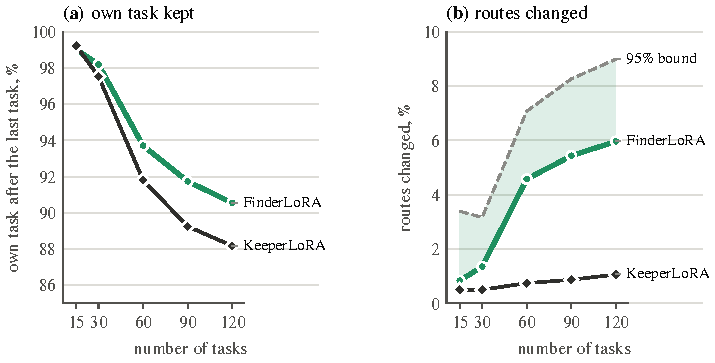
\includegraphics[width=\linewidth]{figures/recogniser_scale}
  \caption{Many tasks, routes only. Left: share of test inputs at their own task after the last task. Right: share of routes changed, with the 95\% bound of the audit for \recog{}. The point at 15 tasks is SuperNI; the others are 30, 60, 90 fresh tasks and all 120 together.}
  \label{fig:recogniserscale}
\end{figure}

\subsection{Trained answers without instructions}
\label{sec:nodeftrained}

\paragraph{Trained answers on a small model.} The stand-alone code (\texttt{t5-small}, the five tasks, no definition, one seed, CPU) was run with the routes of \recog{} on the frozen states of that small model, by the lines of the earlier pilot (Section~\ref{sec:noinstruction}): at most 20 of 200 answers changed and forgetting at most 3 points while more than 100 change with all adapters on; score right after learning at least 90\% of that with all adapters on; at least 80\% of test inputs at their own task. Verdict: ``works''. With all adapters on, \AudSmallAllChanged{} of \AudSmallAllCompared{} answers changed and the score fell from \AudSmallAllLearned{} to \AudSmallAllAP{}; with the routes, \AudSmallRidgeChanged{} of \AudSmallRidgeCompared{} changed, forgetting was \AudSmallRidgeFT{}, the score went from \AudSmallRidgeLearned{} to \AudSmallRidgeAP{}, and 97.2\% reached their own task. Two of the five tasks are learned poorly by this model under either rule, so they add little; the check was planned before the GPU run below and finished after it.

\paragraph{Trained answers: our method against the published methods.} Plain adapters that are never blocked, on a GPU: while task $t$ is learned, adapters $1$ to $t$ are on for all its inputs, and at test time an input is answered by the adapters that existed when the task it is routed to was learned. The routes of \recog{} and \handicap{} ($\nu = 2$) on the frozen T5-base states of the instance were written to the repository before the run (Table~\ref{tab:routesgpu}).
Line fixed before the run: ``beats the published methods in this setting'' if the final score is at least 2 points above the better published method without definitions, forgetting is below 2 points, and at most 32 of the \AudOursRidgeCompared{} compared answers change (a quarter of what GainLoRA changes); ``does not'' if the final score is below that of the better published method or at least \AudPubGainloraNoDefChanged{} answers change; else ``mixed''. Verdict: ``beats the published methods in this setting'', for both. \recog{} ends at \AudOursRidgeAP{} against \AudPubGainloraNoDefAP{} for GainLoRA, with \AudOursRidgeChanged{} of \AudOursRidgeCompared{} answers changed; \handicap{} meets the same three lines (Table~\ref{tab:noinstpublished}). The guesses for \recog{}, 5 to 15 changed answers and forgetting below 1 point, held; they were written before \handicap{} was added.
Limits of this verdict:

(a) The line said ``official test'', but the official test scores plain adapters with all of them on (final score \AudOffOursNoDefAP{}); the routed rules exist only in the re-test, so the re-test is compared with the re-test. The two scorings of the published methods differ little (\AudPubGainloraNoDefAP{} against \AudOffGainloraNoDefAP{} for GainLoRA, \AudPubInfloraNoDefAP{} against \AudOffInfloraNoDefAP{} for InfLoRA).

(b) At 10 epochs most of the gap in the final score is learning, not retention. The guess for our score right after learning, 54 to 58, assumed our adapters would learn as poorly without definitions as the published methods; it was far too low (\AudOursRidgeLearned{}; with all adapters on \AudOursAllLearned{} without definitions and \AudWordOriginalAllLearned{} with; ours learn sst2 and emotion well, the published methods poorly, Table~\ref{tab:noinstpertask}). With a tenth of their published epochs the two methods, which restrict what a new adapter may change, learn two of the five tasks poorly. Forgetting and changed answers are less tied to learning than the final score, but not free of it: forgetting cannot exceed what was learned, and the answers of a method that has learned less may be less stable. The 100-epoch runs below separate learning from retention.

(c) Our final score without any definition is also above the published methods with their definitions (Table~\ref{tab:noinstpublished}), with the same caveat on learning; we had expected GainLoRA with definitions to stay ahead, and it did not.

(d) The audit next to what happened: over the first four tasks the audit of \recog{} says \AudRouteFiveRidgeFirstFourAuditEst{}\% changed on average, with 95\% bounds per task from \AudRouteFiveRidgeFirstFourBoundLow{}\% to \AudRouteFiveRidgeFirstFourBoundHigh{}\%; \AudRouteFiveRidgeChanged{} of \AudRouteFiveRidgeCompared{} routes changed (\AudRouteFiveRidgeChangedShare{}\%), each changed route changed its answer, and no other answer changed. For \handicap{} it is \AudRouteFiveHandicapChanged{} of \AudRouteFiveHandicapCompared{}; the audit is not valid for it on the same held-out inputs (Remark~\ref{rem:auditlimits}(iii)).

(e) Five tasks and a small model, a first sign only. The rule and its setting were chosen on these tasks' test inputs, between variants that differ by at most 1.5 points (Table~\ref{tab:recogniserdev}), so these are development routes; only the fresh batches test the recogniser on tasks it was not chosen on.

\paragraph{Three seeds.} Seeds 43 and 44 were run after the first seed had been read, for the published methods and for ours (the route table is the same in every seed; only the adapters differ).
Line fixed before these runs: the verdict stands for three seeds if the three lines hold for the means and the final score of \recog{} is above that of the better published method in every seed. Verdict: it stands, with the same limits; \recog{} is above in \AudSeedsRidgeAboveInAll{} of \AudSeedsN{} seeds (Table~\ref{tab:noinstseeds}). Its final score is \AudSeedsRidgeAP{} (\AudSeedsRidgeAPLow{} to \AudSeedsRidgeAPHigh{}) against \AudSeedsGainloraAP{} for GainLoRA and \AudSeedsInfloraAP{} for InfLoRA; \AudSeedsRidgeChanged{} of \AudSeedsCompared{} answers changed, against many times more for the published methods; \handicap{} is close to \recog{}.
The guesses (final score 76 to 79 in each seed, 4 to 9 changed answers of 400 for \recog{}, 0 to 3 for \handicap{}) held. The simpler rule \centre{} (nearest centre of word-vectors of the whole input, Section~\ref{sec:method}) ends at \AudSeedsCentreAP{} with \AudSeedsCentreChanged{} changed answers: it goes most of the way; \recog{} and \handicap{} add about three points (the ceiling is \AudSeedsOwnAP{}), fewer changed answers, and the audit and the bound.

\paragraph{The published methods with their published number of epochs.} Point (b) left open whether the two published methods close the gap with full training. Both were run without definitions with \AudFullEpochs{} epochs per task, the published number (seed 42, T5-base; Table~\ref{tab:noinstfull}).
Lines fixed before the run: ``they close the learning gap'' if the score right after learning is at least 73, within five points of ours with 10 epochs, ``they do not'' below 65; ``they hold their answers less well than ours'' if forgetting is at least 5 points above ours or at least 60 more of the \AudFullCompared{} answers change than under \recog{}, ``no such sign'' if forgetting is within 2 points of ours and at most 25 more answers change. Verdict: they close the learning gap, and they hold their answers less well than ours. The two methods learn the tasks as well as plain adapters do at 10 epochs (\AudFullInfloraLearned{} and \AudFullGainloraLearned{} right after learning, against \AudOursRidgeLearned{}), and a little less than plain adapters with \AudFullEpochs{} epochs (\AudFullOursRidgeLearned{}; they now learn sst2 and emotion, Table~\ref{tab:noinstfullpertask}, Appendix~\ref{app:noinstmore}) and then lose them: forgetting \AudFullInfloraFT{} and \AudFullGainloraFT{} points and final scores \AudFullInfloraAP{} and \AudFullGainloraAP{}, with forgetting grown from 10 epochs (Table~\ref{tab:noinstfull}). So at \AudFullEpochs{} epochs the gap in the final score is forgetting, not learning.
The guesses were wrong in the direction of too little forgetting: we expected them to learn 68 to 78 (right; InfLoRA is just above), to change 60 to 200 answers (right for GainLoRA, far too few for InfLoRA) and to forget 4 to 15 points (wrong for both). One seed and five tasks on T5-base, where the published setting uses a larger model.

\paragraph{Our rules with the same number of epochs.} Plain adapters were also trained for \AudFullEpochs{} epochs per task (no definitions, the same route table; top of Table~\ref{tab:noinstfull}).
Line fixed before the run: ``beats the published methods at equal epochs, in this setting'' if the final score of \recog{} is at least 2 points above the better published method at \AudFullEpochs{} epochs, forgetting is below 2 points, and at most 44 of \AudFullCompared{} answers change (a quarter of what GainLoRA changes); ``does not'' if the final score is below that method's. Verdict: all three hold. \recog{} ends at \AudFullOursRidgeAP{}, \AudFullOursRidgeAboveGainlora{} points above GainLoRA, with \AudFullOursRidgeChanged{} changed answers; \handicap{} is close. Right after learning the three are close (Table~\ref{tab:noinstfull}), so at equal training the gap is retention.
Lemma~\ref{lem:route} said in advance that at most as many answers can change as routes, and the routes do not depend on the adapters; here exactly as many answers changed as routes, as at 10 epochs, so ten times the training changed no further answer. Forgetting of \recog{} is \AudFullOursRidgeFT{} points here, above its 10-epoch value: the same inputs go to another task, and a wrong route costs more when the adapters are better.
The guesses held (score right after learning 77 to 82, final score within one point of it, 3 to 6 changed answers); the doubt that more epochs might not help plain adapters was wrong (a rise of \AudFullOursLearnedGain{} points). One seed and five tasks. Figure~\ref{fig:answergrid} shows the changed answers one by one, and Figure~\ref{fig:stageheat} the score of every task after every stage.

\begin{figure}[t]
  \centering
  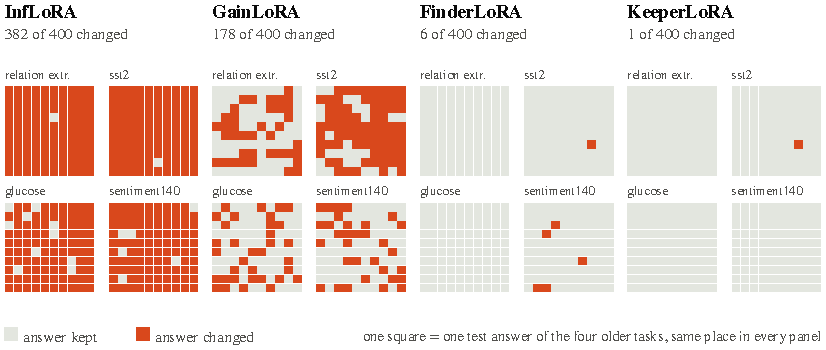
\includegraphics[width=\linewidth]{figures/answer_grid}
  \caption{Every square is one test answer. Five tasks without definitions, \AudFullEpochs{}
  epochs per task, seed 42: the \AudFullCompared{} test answers of the four older tasks, right
  after their task was learned against after the last task; a square has the same place in every
  panel. InfLoRA changes \AudFullInfloraChanged{} of the \AudFullCompared{} answers, GainLoRA
  \AudFullGainloraChanged{}, \recog{} \AudFullOursRidgeChanged{} and \handicap{}
  \AudFullOursHandicapChanged{}.}
  \label{fig:answergrid}
\end{figure}

\begin{figure}[t]
  \centering
  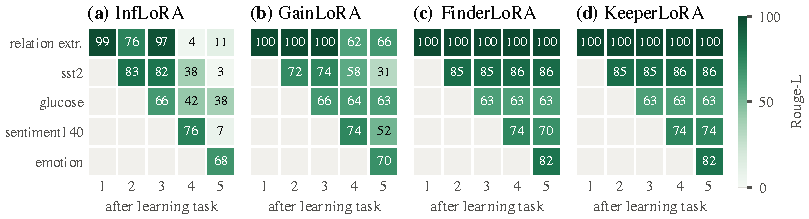
\includegraphics[width=\linewidth]{figures/stage_heatmap}
  \caption{The score of each task (rows) after each later task has been learned (columns), for the
  runs of Figure~\ref{fig:answergrid}; Rouge-L of the re-test (all reference answers), rounded. A
  row that keeps its colour is a task that is not forgotten: with InfLoRA and GainLoRA most rows of
  older tasks fade, with \recog{} and \handicap{} they stay.}
  \label{fig:stageheat}
\end{figure}


\paragraph{The control: the same methods with their definitions.} The loss of the published methods could come from the missing definition or from \AudFullEpochs{} epochs on this smaller model. Both were run with \AudFullEpochs{} epochs and the definitions left in; the definition is the only difference (Table~\ref{tab:fulldefinitions}).
Line fixed before the run, for each method: ``the instruction was what kept the answers'' if, with definitions, forgetting is at most half of its value without and at most half as many answers change; ``it was not the instruction'' if forgetting with definitions is at least 80\% of that without. Verdict: the first holds for both. GainLoRA forgets \AudFullDefOriginalGainloraFT{} points with definitions against \AudFullGainloraFT{} without, InfLoRA \AudFullDefOriginalInfloraFT{} against \AudFullInfloraFT{} (answers changed: Table~\ref{tab:fulldefinitions}). \recog{} and \handicap{}, which never read the definition, forget about one point or less.
With definitions and \AudFullEpochs{} epochs the two end below \cert{} and \recog{} with definitions and 10 epochs (Table~\ref{tab:fullwordings}, Appendix~\ref{app:noinstmore}; Section~\ref{sec:exampleroutes}); we did not train our adapters for \AudFullEpochs{} epochs with definitions. Under the heavy rewording they end lower still, with many more changed answers.
The guesses were right for InfLoRA and for the forgetting of GainLoRA; GainLoRA learned less than guessed (\AudFullDefOriginalGainloraLearned{} right after learning, against 79 to 84), and we had thought it more likely than not to end above our 10-epoch score, which it did not. One seed and five tasks. Figure~\ref{fig:learnkeep} puts the runs with and without definitions side by side.

\begin{figure}[t]
  \centering
  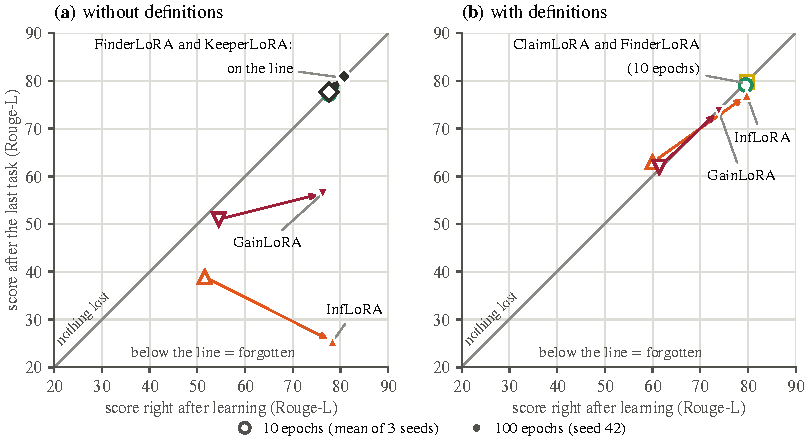
\includegraphics[width=\linewidth]{figures/learn_keep}
  \caption{Learned against kept, five tasks. A point is a method: its mean score right after
  learning ($x$) and after the last task ($y$). On the diagonal nothing is lost; the distance below
  it is what was forgotten. Hollow: 10 epochs (mean of three seeds); filled: \AudFullEpochs{} epochs
  (seed 42); an arrow goes from 10 to \AudFullEpochs{} epochs. (a)~Without definitions the two
  published methods learn more with more epochs and fall further below the diagonal; \recog{} and
  \handicap{} stay on it. (b)~With definitions the published methods stay near the diagonal (the
  control run); for our rules with definitions only 10-epoch runs exist.}
  \label{fig:learnkeep}
\end{figure}


\begin{table}[t]
  \caption{The definition as the only difference: the two published methods with \AudFullEpochs{} epochs per task, with and without definitions (five tasks, seed 42, re-test), and \recog{} and \handicap{} without definitions at the same epochs.}
  \label{tab:fulldefinitions}
  \centering
  {\footnotesize\setlength{\tabcolsep}{3pt}\begin{tabular}{p{1.9in}lrrrr}
    \toprule
    Method (seed 42, 100 epochs) & Definitions & \shortstack[r]{Score right\\after\\learning $\uparrow$} & \shortstack[r]{Final\\score $\uparrow$} & \shortstack[r]{Forgetting\\(points) $\downarrow$} & \shortstack[r]{Answers\\changed\\of \AudFullDefCompared{} $\downarrow$} \\
    \midrule
    InfLoRA & with & \AudFullDefOriginalInfloraLearned{} & \AudFullDefOriginalInfloraAP{} & \AudFullDefOriginalInfloraFT{} & \AudFullDefOriginalInfloraChanged{} \\
    InfLoRA & none & \AudFullInfloraLearned{} & \AudFullInfloraAP{} & \AudFullInfloraFT{} & \AudFullInfloraChanged{} \\
    \midrule
    GainLoRA & with & \AudFullDefOriginalGainloraLearned{} & \AudFullDefOriginalGainloraAP{} & \AudFullDefOriginalGainloraFT{} & \AudFullDefOriginalGainloraChanged{} \\
    GainLoRA & none & \AudFullGainloraLearned{} & \AudFullGainloraAP{} & \AudFullGainloraFT{} & \AudFullGainloraChanged{} \\
    \midrule
    \recog{} (ours) & none & \AudFullOursRidgeLearned{} & \AudFullOursRidgeAP{} & \AudFullOursRidgeFT{} & \AudFullOursRidgeChanged{} \\
    \handicap{} (ours) & none & \AudFullOursHandicapLearned{} & \AudFullOursHandicapAP{} & \AudFullOursHandicapFT{} & \AudFullOursHandicapChanged{} \\
    \bottomrule
\end{tabular}}

\end{table}

\begin{table}[t]
  \caption{The five tasks without definitions, seed 42, re-test: plain adapters behind \recog{} and \handicap{} and the two published methods, each with \AudFullEpochs{} epochs per task (the published number) and with 10. Columns as in Table~\ref{tab:noinstpublished}.}
  \label{tab:noinstfull}
  \centering
  {\footnotesize\setlength{\tabcolsep}{3pt}\begin{tabular}{p{1.95in}rrrr}
    \toprule
    Method, epochs (seed 42, no definition) & \shortstack[r]{Score right\\after\\learning $\uparrow$} & \shortstack[r]{Final\\score $\uparrow$} & \shortstack[r]{Forgetting\\(points) $\downarrow$} & \shortstack[r]{Answers\\changed\\of \AudFullCompared{} $\downarrow$} \\
    \midrule
    \recog{} (ours), 100 epochs & \AudFullOursRidgeLearned{} & \AudFullOursRidgeAP{} & \AudFullOursRidgeFT{} & \AudFullOursRidgeChanged{} \\
    \handicap{} (ours), 100 epochs & \AudFullOursHandicapLearned{} & \AudFullOursHandicapAP{} & \AudFullOursHandicapFT{} & \AudFullOursHandicapChanged{} \\
    \midrule
    InfLoRA, 100 epochs & \AudFullInfloraLearned{} & \AudFullInfloraAP{} & \AudFullInfloraFT{} & \AudFullInfloraChanged{} \\
    GainLoRA, 100 epochs & \AudFullGainloraLearned{} & \AudFullGainloraAP{} & \AudFullGainloraFT{} & \AudFullGainloraChanged{} \\
    \midrule
    InfLoRA, 10 epochs & \AudPubInfloraNoDefLearned{} & \AudPubInfloraNoDefAP{} & \AudPubInfloraNoDefFT{} & \AudPubInfloraNoDefChanged{} \\
    GainLoRA, 10 epochs & \AudPubGainloraNoDefLearned{} & \AudPubGainloraNoDefAP{} & \AudPubGainloraNoDefFT{} & \AudPubGainloraNoDefChanged{} \\
    \midrule
    \recog{} (ours), 10 epochs & \AudOursRidgeLearned{} & \AudOursRidgeAP{} & \AudOursRidgeFT{} & \AudOursRidgeChanged{} \\
    \handicap{} (ours), 10 epochs & \AudOursHandicapLearned{} & \AudOursHandicapAP{} & \AudOursHandicapFT{} & \AudOursHandicapChanged{} \\
    \bottomrule
\end{tabular}}

\end{table}

\begin{table}[t]
  \caption{The five tasks without definitions, means over \AudSeedsN{} seeds (42, 43, 44), re-test, 10 epochs. Final score with the lowest and highest seed; answers changed summed over the seeds. The route table of our rows is the same in every seed. Other columns as in Table~\ref{tab:noinstpublished}.}
  \label{tab:noinstseeds}
  \centering
  {\footnotesize\setlength{\tabcolsep}{2.5pt}\begin{tabular}{lrrrr}
    \toprule
    Method, no definition & \shortstack[r]{Score after\\learning $\uparrow$} & \shortstack[r]{Final\\score $\uparrow$} & \shortstack[r]{Forgetting\\(points) $\downarrow$} & \shortstack[r]{Answers changed\\of \AudSeedsCompared{} $\downarrow$} \\
    \midrule
    InfLoRA & \AudSeedsInfloraLearned{} & \AudSeedsInfloraAP{} {\scriptsize (\AudSeedsInfloraAPLow{}--\AudSeedsInfloraAPHigh{})} & \AudSeedsInfloraFT{} & \AudSeedsInfloraChanged{} \\
    GainLoRA & \AudSeedsGainloraLearned{} & \AudSeedsGainloraAP{} {\scriptsize (\AudSeedsGainloraAPLow{}--\AudSeedsGainloraAPHigh{})} & \AudSeedsGainloraFT{} & \AudSeedsGainloraChanged{} \\
    \midrule
    \plain{} & \AudSeedsPlainLearned{} & \AudSeedsPlainAP{} {\scriptsize (\AudSeedsPlainAPLow{}--\AudSeedsPlainAPHigh{})} & \AudSeedsPlainFT{} & \AudSeedsPlainChanged{} \\
    \centre{} & \AudSeedsCentreLearned{} & \AudSeedsCentreAP{} {\scriptsize (\AudSeedsCentreAPLow{}--\AudSeedsCentreAPHigh{})} & \AudSeedsCentreFT{} & \AudSeedsCentreChanged{} \\
    \recog{} (ours) & \AudSeedsRidgeLearned{} & \AudSeedsRidgeAP{} {\scriptsize (\AudSeedsRidgeAPLow{}--\AudSeedsRidgeAPHigh{})} & \AudSeedsRidgeFT{} & \AudSeedsRidgeChanged{} \\
    \handicap{} (ours) & \AudSeedsHandicapLearned{} & \AudSeedsHandicapAP{} {\scriptsize (\AudSeedsHandicapAPLow{}--\AudSeedsHandicapAPHigh{})} & \AudSeedsHandicapFT{} & \AudSeedsHandicapChanged{} \\
    own task (ceiling) & \AudSeedsOwnLearned{} & \AudSeedsOwnAP{} {\scriptsize (\AudSeedsOwnAPLow{}--\AudSeedsOwnAPHigh{})} & \AudSeedsOwnFT{} & \AudSeedsOwnChanged{} \\
    \bottomrule
\end{tabular}}

\end{table}

\begin{table}[t]
  \caption{Routes of the rules used in the GPU run, for the five-task sequence (500 test inputs, 400 of the first four tasks compared) and for the 15 SuperNI tasks: test inputs not at their own task after the last task; routes changed between arrival and the end, of those compared; audit $H/m$ and 95\% bound (Proposition~\ref{prop:audit}, averaged over all tasks of the sequence), where valid. The last row of each part sends every input to its own task.}
  \label{tab:routesgpu}
  \centering
  {\footnotesize\setlength{\tabcolsep}{3pt}\begin{tabular}{lrrrr}
    \toprule
    Rule & \shortstack[r]{Not sent\\to own task\\at the end $\downarrow$} & \shortstack[r]{Route\\changed $\downarrow$} & \shortstack[r]{Audit\\$H/m$, \%} & \shortstack[r]{95\% bound,\\\%} \\
    \midrule
    \multicolumn{5}{l}{\textit{five-task sequence}} \\
    \recog{} & \AudRouteFiveRidgeNotOwn{} of \AudRouteFiveRidgeN{} & \AudRouteFiveRidgeChanged{} of \AudRouteFiveRidgeCompared{} & \AudRouteFiveRidgeAuditEst{} & \AudRouteFiveRidgeAuditBound{} \\
    \handicap{}, $\nu = 2$ & \AudRouteFiveHandicapNotOwn{} of \AudRouteFiveHandicapN{} & \AudRouteFiveHandicapChanged{} of \AudRouteFiveHandicapCompared{} & -- & -- \\
    \recog{} with logistic regression & \AudRouteFiveJointNotOwn{} of \AudRouteFiveJointN{} & \AudRouteFiveJointChanged{} of \AudRouteFiveJointCompared{} & \AudRouteFiveJointAuditEst{} & \AudRouteFiveJointAuditBound{} \\
    every input to its own task (ceiling) & \AudRouteFiveOwnNotOwn{} of \AudRouteFiveOwnN{} & \AudRouteFiveOwnChanged{} of \AudRouteFiveOwnCompared{} & \AudRouteFiveOwnAuditEst{} & \AudRouteFiveOwnAuditBound{} \\
    \midrule
    \multicolumn{5}{l}{\textit{15 SuperNI tasks}} \\
    \recog{} & \AudRouteFifteenRidgeNotOwn{} of \AudRouteFifteenRidgeN{} & \AudRouteFifteenRidgeChanged{} of \AudRouteFifteenRidgeCompared{} & \AudRouteFifteenRidgeAuditEst{} & \AudRouteFifteenRidgeAuditBound{} \\
    \handicap{}, $\nu = 2$ & \AudRouteFifteenHandicapNotOwn{} of \AudRouteFifteenHandicapN{} & \AudRouteFifteenHandicapChanged{} of \AudRouteFifteenHandicapCompared{} & -- & -- \\
    \recog{} with logistic regression & \AudRouteFifteenJointNotOwn{} of \AudRouteFifteenJointN{} & \AudRouteFifteenJointChanged{} of \AudRouteFifteenJointCompared{} & \AudRouteFifteenJointAuditEst{} & \AudRouteFifteenJointAuditBound{} \\
    every input to its own task (ceiling) & \AudRouteFifteenOwnNotOwn{} of \AudRouteFifteenOwnN{} & \AudRouteFifteenOwnChanged{} of \AudRouteFifteenOwnCompared{} & \AudRouteFifteenOwnAuditEst{} & \AudRouteFifteenOwnAuditBound{} \\
    \bottomrule
\end{tabular}}

\end{table}

\paragraph{Fifteen tasks.} The same run on the 15 SuperNI tasks in their official order (no definitions; Table~\ref{tab:noinstfifteen}). The published methods were not run on fifteen tasks without definitions, so the line for that comparison cannot be read; retention can. Plain adapters behind \recog{} end at \AudFifteenNoDefRidgeAP{}, \AudFifteenNoDefRidgeBelowOwn{} points below the ceiling, with \AudFifteenNoDefRidgeChanged{} of \AudFifteenNoDefCompared{} changed answers; \handicap{} is similar. These are exactly the routes the route table changes (Lemma~\ref{lem:route}); with all adapters on the same adapters end at \AudFifteenNoDefPlainAP{} and every compared answer changes.
The guesses (score right after learning 39 to 43, final score within half a point, 8 to 20 changed answers) held. With definitions and the same epochs the published methods ended far lower, with many more changed answers (Table~\ref{tab:noinstfifteen}, Section~\ref{sec:fifteen}); they had learned less there, so that gap is partly learning. Our score right after learning is the same without definitions as with them (\AudFifteenNoDefOwnLearned{} and \AudFifteenDefCertLearned{}) by chance; the single tasks differ. These are the 15 tasks on which \recog{} was chosen. Figure~\ref{fig:routematrix} shows where the test inputs are sent after the last task.

\begin{figure}[t]
  \centering
  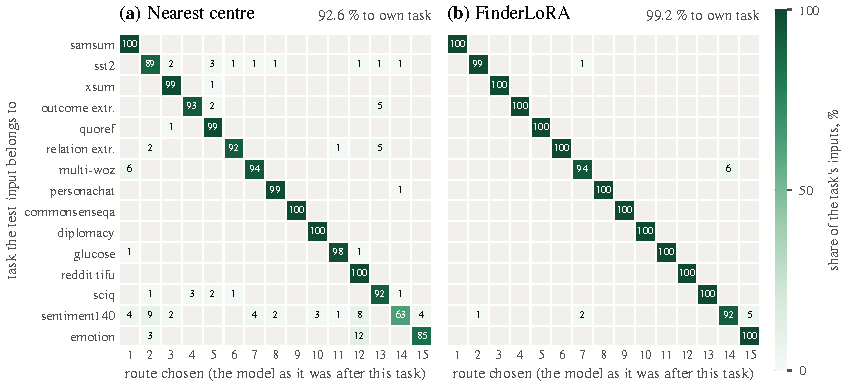
\includegraphics[width=\linewidth]{figures/route_matrix}
  \caption{Where the switch sends the test inputs: fifteen tasks without definitions, after the
  last task (seed 42). Rows: the task an input belongs to; columns: the route it gets; a cell is
  the share of the task's test inputs in per cent (shown from 1\,\%). (a)~The nearest centre sends
  \AudFifteenNoDefCentreRight{}\,\% of the inputs to their own task, (b)~\recog{}
  \AudFifteenNoDefRidgeRight{}\,\%.}
  \label{fig:routematrix}
\end{figure}


\begin{table}[t]
  \caption{The 15 SuperNI tasks without definitions, seed 42, 10 epochs, re-test: the same plain adapters under each rule; columns as in Table~\ref{tab:noinstfull}, last column the share at the own task after the last task. The three bottom rows are the run with definitions of Section~\ref{sec:fifteen}, for reference.}
  \label{tab:noinstfifteen}
  \centering
  {\footnotesize\setlength{\tabcolsep}{3pt}\begin{tabular}{p{1.75in}rrrrr}
    \toprule
    Method (seed 42, 15 tasks) & \shortstack[r]{Score right\\after\\learning $\uparrow$} & \shortstack[r]{Final\\score $\uparrow$} & \shortstack[r]{Forgetting\\(points) $\downarrow$} & \shortstack[r]{Answers\\changed\\of \AudFifteenNoDefCompared{} $\downarrow$} & \shortstack[r]{Sent to own\\task, \% $\uparrow$} \\
    \midrule
    \plain{} & \AudFifteenNoDefPlainLearned{} & \AudFifteenNoDefPlainAP{} & \AudFifteenNoDefPlainFT{} & \AudFifteenNoDefPlainChanged{} & \AudFifteenNoDefPlainRight{} \\
    \centre{} & \AudFifteenNoDefCentreLearned{} & \AudFifteenNoDefCentreAP{} & \AudFifteenNoDefCentreFT{} & \AudFifteenNoDefCentreChanged{} & \AudFifteenNoDefCentreRight{} \\
    \recog{} (ours) & \AudFifteenNoDefRidgeLearned{} & \AudFifteenNoDefRidgeAP{} & \AudFifteenNoDefRidgeFT{} & \AudFifteenNoDefRidgeChanged{} & \AudFifteenNoDefRidgeRight{} \\
    \handicap{} (ours) & \AudFifteenNoDefHandicapLearned{} & \AudFifteenNoDefHandicapAP{} & \AudFifteenNoDefHandicapFT{} & \AudFifteenNoDefHandicapChanged{} & \AudFifteenNoDefHandicapRight{} \\
    every input to its own task (ceiling) & \AudFifteenNoDefOwnLearned{} & \AudFifteenNoDefOwnAP{} & \AudFifteenNoDefOwnFT{} & \AudFifteenNoDefOwnChanged{} & \AudFifteenNoDefOwnRight{} \\
    \midrule
    \cert{}, with definitions & \AudFifteenDefCertLearned{} & \AudFifteenDefCertAP{} & \AudFifteenDefCertFT{} & \AudFifteenDefCertChanged{} & \AudFifteenDefCertRight{} \\
    GainLoRA, with definitions & \AudFifteenDefGainloraLearned{} & \AudFifteenDefGainloraAP{} & \AudFifteenDefGainloraFT{} & \AudFifteenDefGainloraChanged{} & -- \\
    InfLoRA, with definitions & \AudFifteenDefInfloraLearned{} & \AudFifteenDefInfloraAP{} & \AudFifteenDefInfloraFT{} & \AudFifteenDefInfloraChanged{} & -- \\
    \bottomrule
\end{tabular}}

\end{table}

\paragraph{What the results without instructions show.}
\emph{Reached:}
\begin{itemize}
\item A recogniser that reads no instruction, blocks no task, stores one vector per task and one matrix, and is the same for every order of arrival: \AudDevLLamOneEnd{}\% of test inputs at their own task after 15 tasks (development data).
\item An audit and a bound in advance, proved (Proposition~\ref{prop:audit}, Theorem~\ref{thm:handicap}); the measured change was within them in every run (averages over tasks, one split each; on the fresh batches the split does not ensure exchangeability).
\item Three rules passed their lines on fresh tasks, among them \recog{}; it also passed on the second benchmark (\AudScaleLongThreeEnd{}\%, routes only) and gives \AudScaleAllHundredTwentyEnd{}\% with 120 tasks.
\item In one reduced setting, trained answers beat the two published methods without instructions, by the line fixed before (re-test against re-test), at 10 and at \AudFullEpochs{} epochs; at \AudFullEpochs{} epochs the published methods learn the tasks and the gap is forgetting, and the control says the instruction held their answers.
\end{itemize}
\emph{Not reached:}
\begin{itemize}
\item The published setting (a larger model; the full number of epochs for one seed only), and the published methods on more than five tasks without definitions (ours ran on fifteen, one seed).
\item The second benchmark with trained answers; a tight bound in advance.
\item The published methods with an oracle for the task, or with our recogniser in front of them.
\item The upper side of the conflict $\Omega$ (the error of the best classifier between two tasks), and inputs that occur in two tasks, which no method without instructions can do better than split.
\end{itemize}
Choices made after seeing numbers (the features, \handicap{} and its floor, the zone shapes) give development numbers; only the fresh batches and the GPU run were read once against lines written before.

These subsections are about inputs that carry an instruction.

\subsection{Five tasks with instructions: the certified switch}
\label{sec:five}

Five tasks, T5-base, 10 epochs per task, \FiveCertSeeds{} seeds; the answers are re-tested against all reference answers. The following holds for every test in this paper unless a test says otherwise. It is a reduced setting: a tenth of the published budget, a smaller model, and one step of the published methods (a singular value decomposition that the official code delegates to a library that did not load on the free GPUs) computed with PyTorch without a check that the two agree number for number (Appendix~\ref{app:impl}). The five tasks are among the 15 tasks of Section~\ref{sec:fifteen}. The rewordings of the definitions were written by machine during development and looked at during the design (``development rewordings''); they are not rewordings by people. Tests marked ``routes only'' compute where inputs go and train nothing. Statements about InfLoRA and GainLoRA hold only for this setting.

\begin{table}[t]
  \caption{Five-task sequence, original instructions. Score right after learning: average score of each task right after it was learned. AP: average score after the last task. Answers changed: test inputs of the first four
  tasks whose answer at the end differs from the answer right after their task was learned.
  Certified: test inputs inside a zone.
  Scores are means over \FiveCertSeeds{} seeds, with the lowest and the highest seed in brackets; counts are summed over the seeds.}
  \label{tab:fivemain}
  \centering
  \small
  \setlength{\tabcolsep}{4pt}
  \begin{tabular}{lccccc}
    \toprule
    Method & \shortstack[c]{Score\\right after\\learning $\uparrow$} & \shortstack[c]{Final\\score $\uparrow$} & \shortstack[c]{Forgetting\\(points) $\downarrow$} & \shortstack[c]{Answers\\changed $\downarrow$} & Certified inputs \\
    \midrule
    \cert{} (ours) & 79.74 {\scriptsize(79.2--80.8)} & 79.74 {\scriptsize(79.2--80.8)} & 0.00 & 0 of 1{,}200 & 1{,}500 of 1{,}500 \\
    \nearest{} & 79.74 {\scriptsize(79.2--80.8)} & 79.74 {\scriptsize(79.2--80.8)} & 0.00 & 0 of 1{,}200 &  \\
    \centre{} & 79.74 {\scriptsize(79.2--80.8)} & 79.74 {\scriptsize(79.2--80.8)} & 0.00 & 0 of 1{,}200 &  \\
    \keyswitch{} & 79.74 {\scriptsize(79.2--80.8)} & 79.74 {\scriptsize(79.2--80.8)} & 0.00 & 0 of 1{,}200 &  \\
    \plain{} & 79.74 {\scriptsize(79.2--80.8)} & 36.08 {\scriptsize(32.3--39.5)} & 54.58 {\scriptsize(51.6--58.6)} & 994 of 1{,}200 &  \\
    \midrule
    InfLoRA & 60.02 {\scriptsize(56.6--63.3)} & 62.93 {\scriptsize(59.0--65.4)} & $-$3.14 {\scriptsize($-$5.3 to $-$1.7)} & 370 of 1{,}200 &  \\
    GainLoRA & 61.42 {\scriptsize(59.1--64.4)} & 61.96 {\scriptsize(60.9--63.9)} & $-$0.51 {\scriptsize($-$2.6 to 0.7)} & 65 of 1{,}200 &  \\
    \bottomrule
\end{tabular}

\end{table}

\begin{figure}[t]
  \centering
  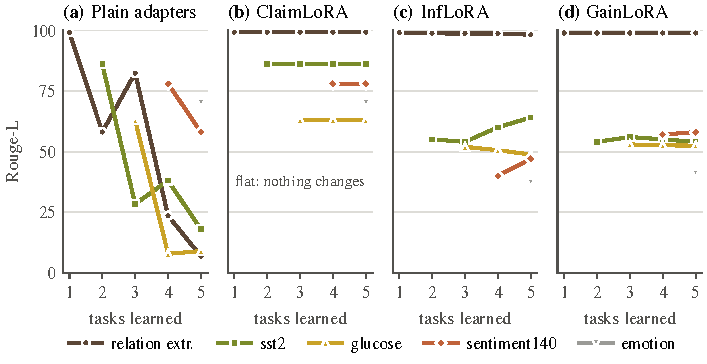
\includegraphics[width=\linewidth]{figures/five_tracks}
  \caption{Score of each of the five tasks as further tasks are learned (seed 42, original
  instructions). Plain adapters fall as soon as the next task is learned; the certified
  switch gives flat lines; the two published methods are flat at a lower level.}
  \label{fig:fivetracks}
\end{figure}

\paragraph{The certified switch keeps every answer.} After the fifth task its average score equals the
score right after learning, \FiveCertAP{} Rouge-L; forgetting is \FiveCertFT{}, and none of
the \FiveCertCompared{} answers to the test inputs of the first four tasks changed. All \FiveCertInputsOne{} test inputs lie inside
their own zone (Proposition~\ref{prop:own}), and no training input of a later
task lay inside an older zone (\FiveCertBlocked{} of \FiveCertTrainInputs{}). This is what Theorem~\ref{thm:writeonce} says; the run confirms that the implementation does what the theorem describes. With the original instructions
\nearest{}, \centre{} and \keyswitch{} choose the same routes and give the same numbers.

\paragraph{The same adapters without a switch lose most of what they learned.} With all adapters on (\plain{}), the average falls to
\FivePlainAP{}, forgetting is \FivePlainFT{} points, and most of the
\FivePlainCompared{} answers change. Only the task learned last is intact.

\paragraph{The published methods learned less here.} InfLoRA and GainLoRA have forgetting scores near zero (\FiveInfFT{} points for InfLoRA; a
negative value means that old tasks improved on average), though \FiveInfChanged{} of \FiveInfCompared{} answers of InfLoRA and \FiveGainChanged{} of \FiveGainCompared{} of GainLoRA change; changes for the better and for the worse cancel in the score. They end at \FiveInfAP{} (InfLoRA),
well below the certified switch, because they are lower from the start: right
after learning they stand at \FiveInfLearned{} and \FiveGainLearned{}, against
\FivePlainLearned{} for plain adapters (Table~\ref{tab:fivemain}). Both learn relation extraction but not the classification tasks within ten epochs; on SST-2 and Sentiment140 they are at the level of guessing right after learning (Table~\ref{tab:instdetail}). \textbf{So in our runs these two methods were at the level of guessing on two of the five tasks and clearly below plain adapters on a third, and the comparison cannot show how well they retain what they learn.} We do not know how much of this is the method and how much is our set-up.

\paragraph{Official script, and the same seed twice.} The scores of the official script (one randomly picked reference per input) lead to the same reading as the re-test (Table~\ref{tab:fiveofficial}; agreement of the answers in Table~\ref{tab:instdetail}). Seed 42 was run twice in separate sessions on the same kind of GPU: the first task was reproduced answer for answer (for \cert{} and InfLoRA also the second), the later ones were not, so training is not reproducible bit for bit and differences of a few tenths of a point mean nothing. The count for the certified switch does not vary: no answer of an earlier task changed in either run, nor in any other seed. The tables use the second run, made together with seeds 43 and 44.

\subsection{Reworded instructions}
\label{sec:reworded}

\begin{table}[t]
  \caption{Five tasks with the original and with three levels of rewording: average score at the end and
  number of changed answers. The adapters are those of Table~\ref{tab:fivemain}; nothing is
  retrained. Means and sums over the seeds.}
  \label{tab:fivewordings}
  \centering
  \small
  \setlength{\tabcolsep}{4.5pt}
  \begin{tabular}{lcccccccc}
    \toprule
    & \multicolumn{4}{c}{Final score $\uparrow$} & \multicolumn{4}{c}{Answers changed (of 1{,}200) $\downarrow$} \\
    \cmidrule(lr){2-5} \cmidrule(lr){6-9}
    Method & original & light & medium & heavy & original & light & medium & heavy \\
    \midrule
    \cert{} (ours) & 79.7 & 79.6 & 79.0 & 74.1 & 0 & 0 & 0 & 0 \\
    \nearest{} & 79.7 & 79.6 & 79.0 & 74.1 & 0 & 0 & 0 & 0 \\
    \centre{} & 79.7 & 79.6 & 78.4 & 59.4 & 0 & 0 & 0 & 171 \\
    \keyswitch{} & 79.7 & 36.4 & 36.0 & 35.2 & 0 & 985 & 1{,}001 & 939 \\
    \plain{} & 36.1 & 36.4 & 36.0 & 35.2 & 994 & 985 & 1{,}001 & 939 \\
    \midrule
    InfLoRA & 62.9 & 64.3 & 57.8 & 54.3 & 370 & 296 & 320 & 470 \\
    GainLoRA & 62.0 & 64.6 & 58.8 & 51.6 & 65 & 58 & 122 & 178 \\
    \bottomrule
\end{tabular}

\end{table}

\begin{figure}[t]
  \centering
  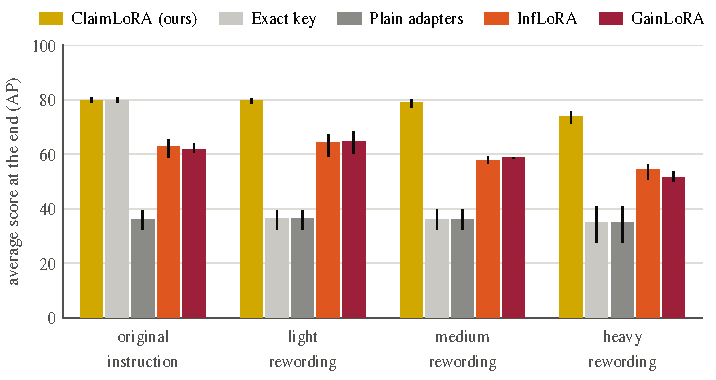
\includegraphics[width=0.9\linewidth]{figures/five_wordings}
  \caption{Average score at the end (AP) on the five tasks, original instructions and
  three levels of rewording. Bars are means over seeds; a black line spans the lowest and the highest seed.}
  \label{fig:fivewordings}
\end{figure}

\begin{table}[t]
  \caption{Routes on the five tasks: test inputs that are certified, given to
  their own task, and whose answers change, for the certified switch and for the nearest-centre
  rule. Routes do not depend on the seed; counts are summed over seeds.}
  \label{tab:fiveroutes}
  \centering
  \small
  \setlength{\tabcolsep}{4.5pt}
  \begin{tabular}{lcccccc}
    \toprule
    & & \multicolumn{3}{c}{\cert{}} & \multicolumn{2}{c}{\centre{}} \\
    \cmidrule(lr){3-5} \cmidrule(lr){6-7}
    Wording & Tasks & Certified inputs & \shortstack[c]{Sent to own\\task $\uparrow$} & \shortstack[c]{Answers\\changed $\downarrow$} & \shortstack[c]{Sent to own\\task $\uparrow$} & \shortstack[c]{Answers\\changed $\downarrow$} \\
    \midrule
    original & 5 & 1{,}500 of 1{,}500 & 100.0\% & 0 of 1{,}200 & 100.0\% & 0 of 1{,}200 \\
    light & 5 & 1{,}500 of 1{,}500 & 100.0\% & 0 of 1{,}200 & 100.0\% & 0 of 1{,}200 \\
    medium & 5 & 300 of 1{,}500 & 100.0\% & 0 of 1{,}200 & 99.2\% & 0 of 1{,}200 \\
    heavy & 5 & 294 of 1{,}500 & 93.8\% & 0 of 1{,}200 & 72.2\% & 171 of 1{,}200 \\
    \bottomrule
\end{tabular}

\end{table}

A benchmark input carries its task definition word for word, so any rule that recognises the
definition looks perfect. The test that separates the rules asks the same task in other
words: the evaluation is repeated with the light, medium and heavy rewording of each definition.

\paragraph{No answer changes under any wording.} For the certified switch the count of changed answers is zero in every column. For the light rewording this is guaranteed, because all \FiveCertZoneOneLight{} inputs are
still certified. For the medium and the heavy rewording it is not: only \FiveCertZoneOneMedium{} and \FiveCertZoneOneHeavy{} of the \FiveCertInputsOne{}
inputs are inside a zone, all of relation extraction, the task with the longest instruction. The others kept their answers because no later task came nearer to them than
their own, which Proposition~\ref{prop:uncertified} permits but does not
promise; in an order where SST-2 is learned after
Sentiment140, 31 routes of heavily reworded inputs would change (Section~\ref{sec:orders}). The average
score falls from \FiveCertAP{} to \FiveCertAPHeavy{} at the heavy wording (Table~\ref{tab:fivewordings}, Figure~\ref{fig:fivewordings}).

\paragraph{Other rules.} \keyswitch{} compares the opening token for token: with the light rewording it recognises nothing, leaves
all adapters on and ends where \plain{} ends. \nearest{} and \cert{} score alike on this benchmark; the radius decides which inputs also carry the guarantee. \centre{}, the nearest-centre rule with the token weights of Eq.~\eqref{eq:weights}, gives only
\FiveCentreRightHeavy{}\% of the heavily reworded inputs to their own task, scores far below \cert{} and
changes answers as later tasks arrive (Tables~\ref{tab:fivewordings}, \ref{tab:fiveroutes}; \FiveCentreComparedHeavy{} answers compared). The first version of \cert{}, the nearest centre
with all tokens weighted equally, did better here (97.4\% to the right task with seed 42, against
\FiveCertRightHeavy{}\% for the final rule) and was replaced because it failed on the 15-task sequence (Appendix~\ref{app:history}). The published methods have no recognition step that a rewording could break; their forgetting scores stay within a few points in every wording, and the most answers differ under heavy rewording (Table~\ref{tab:fivewordings}, of \FiveInfComparedHeavy{}).

\paragraph{Where the loss under heavy rewording comes from.} None of the drop from \FiveCertAP{} to \FiveCertAPHeavy{} is forgetting. One part is that the adapters answer
a reworded instruction less well: with all adapters on, right after each task, the score is
\FivePlainLearnedHeavy{}. The other part is routing:
\FiveCertWrongHeavy{} of the \FiveCertInputsOne{} heavily reworded inputs go to another task,
which brings \FivePlainLearnedHeavy{} down to the final \FiveCertAPHeavy{}. All of them are tweets of
Sentiment140 given to SST-2, the other sentiment task.

\begin{figure}[t]
  \centering
  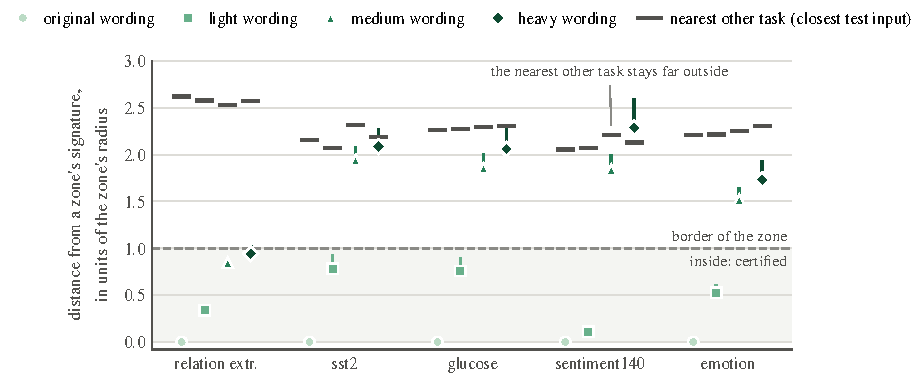
\includegraphics[width=0.92\linewidth]{figures/margins}
  \caption{Why rewording costs the certificate before it costs the route (five tasks, T5-base
  word-vectors). Markers: relative distance $\delta_k$ of the test inputs of a task from their own
  signature, in units of the radius of their own zone: median over the 100 inputs, with a line up to
  the farthest input. Short dark lines: how close the closest of these inputs comes to the signature of any
  \emph{other} task, in units of that task's radius. Below the dashed line an input is inside the
  zone, that is, certified.}
  \label{fig:margins}
\end{figure}

\paragraph{Where reworded inputs lie.}\label{sec:geometry} With the original
wording every input lies exactly on the signature of its task (Proposition~\ref{prop:own}). The
light rewordings move inputs by 0.1 to 0.8 radii, inside the zone. The medium and heavy
rewordings move them by 1.5 to 2.3 radii in four of the five tasks, outside; relation
extraction stays inside. The signatures of the other tasks are 2.1 to 2.6 of \emph{their} radii away, so an input that has left its
zone is mostly still nearer to its own signature than to any other: the
certificate is lost long before the route. The margins cross where the errors are: under heavy rewording the tweets of Sentiment140 lie 2.29 radii from their
own signature (up to 2.60), and the signature of SST-2 is 2.13 of its
radii from the closest of them (Appendix~\ref{app:more}, Table~\ref{tab:geometry}).

\subsection{Routes from the example alone: rewording cannot change the route}
\label{sec:exampleroutes}

Under heavy rewording \cert{} sends some inputs to another task (Section~\ref{sec:reworded}), while \recog{} never
reads the instruction (Remark~\ref{rem:auditlimits}(v)). The five tasks were trained once more
with their definitions (plain adapters, nothing blocked); \recog{} and
\handicap{} route from the example alone, with the route table of the runs without
instructions (Section~\ref{sec:nodeftrained}). The scores of \cert{} equal those of the single-seed run of seed 42 with definitions, not those of the three-seed run of Table~\ref{tab:fivewordings} (seed 42 was trained twice; Section~\ref{sec:five}).

\begin{table}[t]
  \caption{The five tasks with their definitions, seed 42, plain adapters; the
  same adapters under each rule, at the four wordings. Top: final score (AP).
  Bottom: answers of the first four tasks that differ at the end, of \AudUCompared{}. ``Zone first'': the certified route where the input is
  inside a zone, otherwise the route of \recog{} or \handicap{}. The rows of the published
  methods are from Section~\ref{sec:reworded}.}
  \label{tab:instanceroutes}
  \centering
  {\scriptsize\setlength{\tabcolsep}{2pt}\begin{tabular}{p{1.2in}rrrrrrrrr}
    \toprule
    & \multicolumn{4}{c}{Final score $\uparrow$} & \multicolumn{4}{c}{\shortstack{Answers changed\\of \AudUCompared{} $\downarrow$}} & \shortstack[r]{Sent to own\\task, heavy, \% $\uparrow$} \\
    \cmidrule(lr){2-5}\cmidrule(lr){6-9}
    & original & light & medium & heavy & original & light & medium & heavy & \\
    \midrule
    \cert{} (zones on the instruction) & \AudUOriginalCertAP{} & \AudULightCertAP{} & \AudUMediumCertAP{} & \AudUHeavyCertAP{} & \AudUOriginalCertChanged{} & \AudULightCertChanged{} & \AudUMediumCertChanged{} & \AudUHeavyCertChanged{} & \AudUHeavyCertRight{} \\
    \recog{} (example alone) & \AudUOriginalRidgeAP{} & \AudULightRidgeAP{} & \AudUMediumRidgeAP{} & \AudUHeavyRidgeAP{} & \AudUOriginalRidgeChanged{} & \AudULightRidgeChanged{} & \AudUMediumRidgeChanged{} & \AudUHeavyRidgeChanged{} & \AudUHeavyRidgeRight{} \\
    \handicap{}, $\nu = 2$ (example alone) & \AudUOriginalHandicapAP{} & \AudULightHandicapAP{} & \AudUMediumHandicapAP{} & \AudUHeavyHandicapAP{} & \AudUOriginalHandicapChanged{} & \AudULightHandicapChanged{} & \AudUMediumHandicapChanged{} & \AudUHeavyHandicapChanged{} & \AudUHeavyHandicapRight{} \\
    every input to its own task (ceiling) & \AudUOriginalOwnAP{} & \AudULightOwnAP{} & \AudUMediumOwnAP{} & \AudUHeavyOwnAP{} & \AudUOriginalOwnChanged{} & \AudULightOwnChanged{} & \AudUMediumOwnChanged{} & \AudUHeavyOwnChanged{} & \AudUHeavyOwnRight{} \\
    zone first, else \recog{} & \AudUOriginalMixRidgeAP{} & \AudULightMixRidgeAP{} & \AudUMediumMixRidgeAP{} & \AudUHeavyMixRidgeAP{} & \AudUOriginalMixRidgeChanged{} & \AudULightMixRidgeChanged{} & \AudUMediumMixRidgeChanged{} & \AudUHeavyMixRidgeChanged{} & \AudUHeavyMixRidgeRight{} \\
    zone first, else \handicap{} & \AudUOriginalMixHandicapAP{} & \AudULightMixHandicapAP{} & \AudUMediumMixHandicapAP{} & \AudUHeavyMixHandicapAP{} & \AudUOriginalMixHandicapChanged{} & \AudULightMixHandicapChanged{} & \AudUMediumMixHandicapChanged{} & \AudUHeavyMixHandicapChanged{} & \AudUHeavyMixHandicapRight{} \\
    \centre{} & \AudUOriginalCentreAP{} & \AudULightCentreAP{} & \AudUMediumCentreAP{} & \AudUHeavyCentreAP{} & \AudUOriginalCentreChanged{} & \AudULightCentreChanged{} & \AudUMediumCentreChanged{} & \AudUHeavyCentreChanged{} & \AudUHeavyCentreRight{} \\
    \plain{} & \AudUOriginalPlainAP{} & \AudULightPlainAP{} & \AudUMediumPlainAP{} & \AudUHeavyPlainAP{} & \AudUOriginalPlainChanged{} & \AudULightPlainChanged{} & \AudUMediumPlainChanged{} & \AudUHeavyPlainChanged{} & \AudUHeavyPlainRight{} \\
    \midrule
    GainLoRA & \AudWordOriginalGainloraAP{} & \AudWordLightGainloraAP{} & \AudWordMediumGainloraAP{} & \AudWordHeavyGainloraAP{} & \AudWordOriginalGainloraChanged{} & \AudWordLightGainloraChanged{} & \AudWordMediumGainloraChanged{} & \AudWordHeavyGainloraChanged{} & -- \\
    InfLoRA & \AudWordOriginalInfloraAP{} & \AudWordLightInfloraAP{} & \AudWordMediumInfloraAP{} & \AudWordHeavyInfloraAP{} & \AudWordOriginalInfloraChanged{} & \AudWordLightInfloraChanged{} & \AudWordMediumInfloraChanged{} & \AudWordHeavyInfloraChanged{} & -- \\
    \bottomrule
\end{tabular}}

\end{table}

\paragraph{Seed 42.} Line fixed before the run: \recog{} ``repairs the weak spot'' if its final score at the heavy
wording is at least 2 points above that of \cert{}, its score at the original wording is within
2 points of \cert{}, and at most 8 of the \AudUCompared{} compared answers change at every wording;
it ``does not'' if the heavy score is below that of \cert{} or the original score more than 4
points below. Verdict: all three lines hold (Table~\ref{tab:instanceroutes}). At the heavy wording \recog{} ends at
\AudUHeavyRidgeAP{}, and \handicap{} close to it, above \cert{}; the ceiling, with every input at its own task, is \AudUHeavyOwnAP{}. Our guesses (78.5 to 79.3 at the original wording, 75.5 to 76.7 at the heavy one) held. One was wrong in the good direction: we expected about six changed answers for \recog{}, as without definitions; six routes change, but for three
of these inputs the model gives the same answer with the adapters up to either task, and why fewer answers change with the definition we did not test. The routes of \recog{} are the same at every wording, so it stays
\AudURidgeBelowOwnLow{} to \AudURidgeBelowOwnHigh{} points below the ceiling (\handicap{}: \AudUHandicapBelowOwnLow{} to \AudUHandicapBelowOwnHigh{}): what is lost
under rewording is what the adapters themselves lose, not misrouting, while \cert{} loses
\AudUHeavyCertBelowOwn{} points at the heavy wording through misrouted
inputs. The mixed rule is best at the original, light and heavy wording and below \cert{} at the medium one, whose own fallback is right for every input there.

\paragraph{Three seeds.} An independent reading pointed out that seed 42 is the seed in which \cert{} loses most at the heavy wording, so seeds 43 and 44 were added (Table~\ref{tab:instanceroutesseeds}).
Line fixed before these runs, for the means over the three seeds: the result ``stands for three seeds'' if the heavy score of \recog{} is at least 2 points above that of \cert{}, the original score is within 2 points of \cert{}, and in every seed at most 8 of \AudUCompared{} answers change at every wording.
Verdict: it stands. At the heavy wording \recog{} ends at \AudUThreeHeavyRidgeAP{}, a gain of \AudUThreeHeavyRidgeAboveCert{} points over \cert{}; at the original wording it is \AudUThreeOriginalRidgeBelowCert{} points below \cert{}; in no seed and at no wording do more than \AudUThreeMaxChangedPerSeed{} answers change under \recog{}. Over the four wordings \recog{} stays \AudUThreeRidgeBelowOwnLow{} to \AudUThreeRidgeBelowOwnHigh{} points below the ceiling and \handicap{} \AudUThreeHandicapBelowOwnLow{} to \AudUThreeHandicapBelowOwnHigh{}; \cert{} loses \AudUThreeHeavyCertBelowOwn{} points at the heavy wording.
We had expected a smaller gain, 2 to 2.5 points: in seeds 43 and 44 the adapters lose less under heavy rewording than in seed 42.
These three seeds are not the training runs of Table~\ref{tab:fivewordings}: seed 42 is the single-seed run, and seeds 43 and 44 were trained again. So \cert{} ends at \AudUThreeOriginalCertAPOne{} (original) and \AudUThreeHeavyCertAPOne{} (heavy) here, and at \FiveCertAP{} and \FiveCertAPHeavy{} in Table~\ref{tab:fivewordings}; the difference is of the size seen between two runs of the same seed.
It remains five tasks, with three development rewordings per task, not rewordings by people; Remark~\ref{rem:auditlimits}(v) says what this assumes about the input.

\begin{table}[t]
  \caption{As Table~\ref{tab:instanceroutes}, means over \AudUThreeSeeds{} seeds (42, 43, 44); changed answers are summed over the seeds. Training runs: seed 42 as in Table~\ref{tab:instanceroutes}, seeds 43 and 44 trained for this table; they are not the runs of Table~\ref{tab:fivewordings}, so the rows of \cert{} differ from it by a few tenths of a point.}
  \label{tab:instanceroutesseeds}
  \centering
  {\scriptsize\setlength{\tabcolsep}{2pt}\begin{tabular}{p{1.2in}rrrrrrrrr}
    \toprule
    & \multicolumn{4}{c}{Final score $\uparrow$} & \multicolumn{4}{c}{\shortstack{Answers changed\\of \AudUThreeCompared{} $\downarrow$}} & \shortstack[r]{Sent to own\\task, heavy, \% $\uparrow$} \\
    \cmidrule(lr){2-5}\cmidrule(lr){6-9}
    & original & light & medium & heavy & original & light & medium & heavy & \\
    \midrule
    \cert{} (zones on the instruction) & \AudUThreeOriginalCertAP{} & \AudUThreeLightCertAP{} & \AudUThreeMediumCertAP{} & \AudUThreeHeavyCertAP{} & \AudUThreeOriginalCertChanged{} & \AudUThreeLightCertChanged{} & \AudUThreeMediumCertChanged{} & \AudUThreeHeavyCertChanged{} & \AudUThreeHeavyCertRight{} \\
    \recog{} (example alone) & \AudUThreeOriginalRidgeAP{} & \AudUThreeLightRidgeAP{} & \AudUThreeMediumRidgeAP{} & \AudUThreeHeavyRidgeAP{} & \AudUThreeOriginalRidgeChanged{} & \AudUThreeLightRidgeChanged{} & \AudUThreeMediumRidgeChanged{} & \AudUThreeHeavyRidgeChanged{} & \AudUThreeHeavyRidgeRight{} \\
    \handicap{}, $\nu = 2$ (example alone) & \AudUThreeOriginalHandicapAP{} & \AudUThreeLightHandicapAP{} & \AudUThreeMediumHandicapAP{} & \AudUThreeHeavyHandicapAP{} & \AudUThreeOriginalHandicapChanged{} & \AudUThreeLightHandicapChanged{} & \AudUThreeMediumHandicapChanged{} & \AudUThreeHeavyHandicapChanged{} & \AudUThreeHeavyHandicapRight{} \\
    every input to its own task (ceiling) & \AudUThreeOriginalOwnAP{} & \AudUThreeLightOwnAP{} & \AudUThreeMediumOwnAP{} & \AudUThreeHeavyOwnAP{} & \AudUThreeOriginalOwnChanged{} & \AudUThreeLightOwnChanged{} & \AudUThreeMediumOwnChanged{} & \AudUThreeHeavyOwnChanged{} & \AudUThreeHeavyOwnRight{} \\
    zone first, else \recog{} & \AudUThreeOriginalMixRidgeAP{} & \AudUThreeLightMixRidgeAP{} & \AudUThreeMediumMixRidgeAP{} & \AudUThreeHeavyMixRidgeAP{} & \AudUThreeOriginalMixRidgeChanged{} & \AudUThreeLightMixRidgeChanged{} & \AudUThreeMediumMixRidgeChanged{} & \AudUThreeHeavyMixRidgeChanged{} & \AudUThreeHeavyMixRidgeRight{} \\
    zone first, else \handicap{} & \AudUThreeOriginalMixHandicapAP{} & \AudUThreeLightMixHandicapAP{} & \AudUThreeMediumMixHandicapAP{} & \AudUThreeHeavyMixHandicapAP{} & \AudUThreeOriginalMixHandicapChanged{} & \AudUThreeLightMixHandicapChanged{} & \AudUThreeMediumMixHandicapChanged{} & \AudUThreeHeavyMixHandicapChanged{} & \AudUThreeHeavyMixHandicapRight{} \\
    \centre{} & \AudUThreeOriginalCentreAP{} & \AudUThreeLightCentreAP{} & \AudUThreeMediumCentreAP{} & \AudUThreeHeavyCentreAP{} & \AudUThreeOriginalCentreChanged{} & \AudUThreeLightCentreChanged{} & \AudUThreeMediumCentreChanged{} & \AudUThreeHeavyCentreChanged{} & \AudUThreeHeavyCentreRight{} \\
    \plain{} & \AudUThreeOriginalPlainAP{} & \AudUThreeLightPlainAP{} & \AudUThreeMediumPlainAP{} & \AudUThreeHeavyPlainAP{} & \AudUThreeOriginalPlainChanged{} & \AudUThreeLightPlainChanged{} & \AudUThreeMediumPlainChanged{} & \AudUThreeHeavyPlainChanged{} & \AudUThreeHeavyPlainRight{} \\
    \midrule
    GainLoRA & \AudUThreeOriginalGainloraAP{} & \AudUThreeLightGainloraAP{} & \AudUThreeMediumGainloraAP{} & \AudUThreeHeavyGainloraAP{} & \AudUThreeOriginalGainloraChanged{} & \AudUThreeLightGainloraChanged{} & \AudUThreeMediumGainloraChanged{} & \AudUThreeHeavyGainloraChanged{} & -- \\
    InfLoRA & \AudUThreeOriginalInfloraAP{} & \AudUThreeLightInfloraAP{} & \AudUThreeMediumInfloraAP{} & \AudUThreeHeavyInfloraAP{} & \AudUThreeOriginalInfloraChanged{} & \AudUThreeLightInfloraChanged{} & \AudUThreeMediumInfloraChanged{} & \AudUThreeHeavyInfloraChanged{} & -- \\
    \bottomrule
\end{tabular}}

\end{table}

\subsection{Fifteen tasks with instructions}
\label{sec:fifteen}

The five-task sequence was chosen by us. To test a sequence we did not choose, the 15 tasks of the official order~1 of Super-NaturalInstructions were run with the same
model, budget and code, for the certified switch and the two published methods: one seed, 3.1 to 3.5 hours per run on a free GPU.

\begin{table}[t]
  \caption{Fifteen-task sequence, original instructions (seed 42; columns as in Table~\ref{tab:fivemain}). ``Changed'' counts
  test inputs of the first 14 tasks.}
  \label{tab:fifteenmain}
  \centering
  \small
  \setlength{\tabcolsep}{4pt}
  \begin{tabular}{lccccc}
    \toprule
    Method & \shortstack[c]{Score\\right after\\learning $\uparrow$} & \shortstack[c]{Final\\score $\uparrow$} & \shortstack[c]{Forgetting\\(points) $\downarrow$} & \shortstack[c]{Answers\\changed $\downarrow$} & Certified inputs \\
    \midrule
    \cert{} (ours) & 42.77 & 42.77 & 0.00 & 0 of 1{,}097 & 1{,}197 of 1{,}197 \\
    \nearest{} & 42.77 & 42.77 & 0.00 & 0 of 1{,}097 &  \\
    \centre{} & 42.77 & 42.63 & 0.15 & 2 of 1{,}097 &  \\
    \keyswitch{} & 42.77 & 42.77 & 0.00 & 0 of 1{,}097 &  \\
    \plain{} & 42.77 & 14.88 & 30.67 & 973 of 1{,}097 &  \\
    \midrule
    InfLoRA & 30.46 & 26.13 & 5.69 & 661 of 1{,}097 &  \\
    GainLoRA & 29.08 & 28.62 & 1.09 & 215 of 1{,}097 &  \\
    \bottomrule
\end{tabular}

\end{table}

\begin{figure}[t]
  \centering
  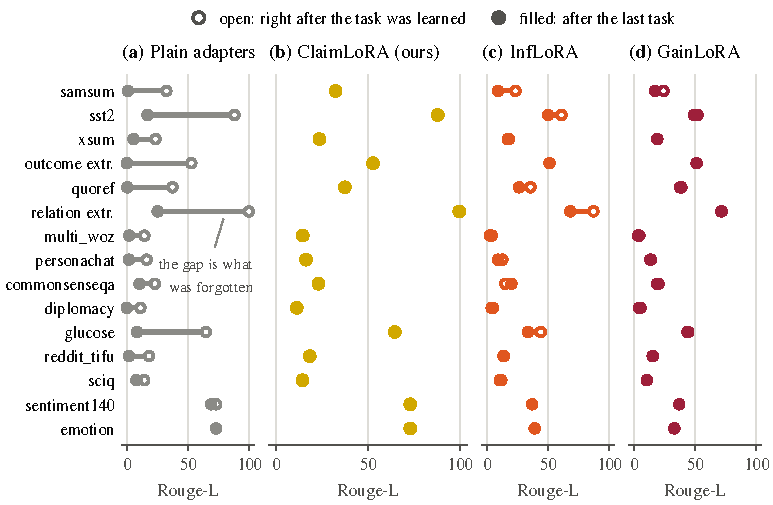
\includegraphics[width=\linewidth]{figures/fifteen_tasks}
  \caption{Score of each of the 15 tasks for four methods. Open circle: right after the task was
  learned. Filled circle: after the last task. For the
  certified switch the two circles coincide for every task.}
  \label{fig:fifteentasks}
\end{figure}

\paragraph{The certified switch keeps every answer.} Its average score after the 15th task equals
the score right after learning, \FifteenCertAP{} Rouge-L; forgetting is \FifteenCertFT{},
and none of the \FifteenCertCompared{} answers of the first 14 tasks changed. All \FifteenCertInputsOne{} test inputs lie
inside their own zone and no training input of a later task lay inside an older zone
(\FifteenCertBlocked{} of \FifteenCertTrainInputs{}), as Theorem~\ref{thm:writeonce}
guarantees. \nearest{} and \keyswitch{} give the same numbers, so
simpler rules reach the same score on this benchmark; \centre{} changes \FifteenCentreChanged{}
answers. With all adapters on the average falls to \FifteenPlainAP{} (forgetting \FifteenPlainFT{} points; most of \FifteenPlainCompared{} answers change), and every task except the last falls (Table~\ref{tab:fifteenpertask}).

\paragraph{The published methods learned less, and on fifteen tasks they also forget.} InfLoRA and
GainLoRA end at \FifteenInfAP{} and \FifteenGainAP{}. On five tasks
neither forgot; here InfLoRA forgets \FifteenInfFT{} points and GainLoRA \FifteenGainFT{}, and
\FifteenInfChanged{} (InfLoRA) and \FifteenGainChanged{} (GainLoRA) of \FifteenInfCompared{} answers differ at the end (Table~\ref{tab:fifteenmain}). The forgetting of InfLoRA is not
spread evenly (relation extraction, SST-2, SAMSum and Glucose fall most; Table~\ref{tab:instdetail}). Both
methods also learned less right after each task, \FifteenInfLearned{} and \FifteenGainLearned{}, against
\FifteenPlainLearned{} for plain adapters, so the gap to the
certified switch has two parts, a gap in learning and a smaller gap from forgetting (Section~\ref{sec:gap}). The official-script scores of InfLoRA are identical to those of an earlier run of the same method on Google Colab with the same seed (unlike the two five-task runs of seed 42, \fivefull{}).

\paragraph{The official script shows forgetting where no answer changed.} The official script gives
the certified switch an AP of \FifteenCertOffAP{} and a forgetting of \FifteenCertOffFT{}
(Table~\ref{tab:fifteenofficial}), although no answer changes. This is evaluation noise: the script scores each answer against one reference picked at random
on every load, and the re-test, which scores against all references, finds that none of the answers changed (agreement in Table~\ref{tab:instdetail}). When the claim is that nothing changed, the answers have to be
compared and not the scores. The official scores of InfLoRA and GainLoRA (AP \FifteenInfOffAP{} and \FifteenGainOffAP{}) lead to the same reading as
the re-test.

\begin{table}[t]
  \caption{Fifteen-task sequence with the original and with reworded instructions. The five tasks
  with rewordings sit inside the 15-task sequence. AP is the average score of these five tasks after the last task; ``Answers changed'' counts
  test inputs of the first four of them (of 400), and in the column ``original'' those of the first 14 tasks of the whole sequence (of 1{,}097). The adapters are those of Table~\ref{tab:fifteenmain};
  nothing is retrained.}
  \label{tab:fifteenwordings}
  \centering
  \small
  \setlength{\tabcolsep}{3.5pt}
  \begin{tabular}{lcccccccc}
    \toprule
    & \multicolumn{4}{c}{Final score $\uparrow$} & \multicolumn{4}{c}{Answers changed $\downarrow$} \\
    \cmidrule(lr){2-5} \cmidrule(lr){6-9}
    Method & original & light & medium & heavy & original & light & medium & heavy \\
    \midrule
    \cert{} (ours) & 42.8 & 80.7 & 80.2 & 76.0 & 0 & 0 & 0 & 0 \\
    \nearest{} & 42.8 & 80.7 & 80.2 & 76.0 & 0 & 0 & 0 & 0 \\
    \centre{} & 42.6 & 80.7 & 72.0 & 57.5 & 2 & 0 & 29 & 100 \\
    \keyswitch{} & 42.8 & 39.6 & 40.4 & 36.1 & 0 & 316 & 313 & 310 \\
    \plain{} & 14.9 & 39.6 & 40.4 & 36.1 & 973 & 316 & 313 & 310 \\
    \midrule
    InfLoRA & 26.1 & 51.6 & 44.7 & 32.6 & 661 & 257 & 272 & 270 \\
    GainLoRA & 28.6 & 51.1 & 47.1 & 37.0 & 215 & 69 & 85 & 109 \\
    \bottomrule
\end{tabular}

\end{table}

\paragraph{Reworded instructions inside the long sequence.} Table~\ref{tab:fifteenwordings} repeats
the test of Section~\ref{sec:reworded} inside the 15-task sequence; this does not make
the development rewordings an independent test. For the certified switch the count of changed answers is zero in every wording; the guarantee covers all inputs of the light rewording but only part of the medium and heavy ones, so the zero is not guaranteed there. The \centre{} rule fails here, with \FifteenCentreChangedMedium{} and \FifteenCentreChangedHeavy{} of \FifteenCentreComparedHeavy{} answers changed, and the exact key ends where plain adapters end. Other numbers are in Table~\ref{tab:instdetail} (further detail in Table~\ref{tab:fifteenmore}).

\subsection{Where the gap to the published methods comes from}
\label{sec:gap}

\begin{figure}[t]
  \centering
  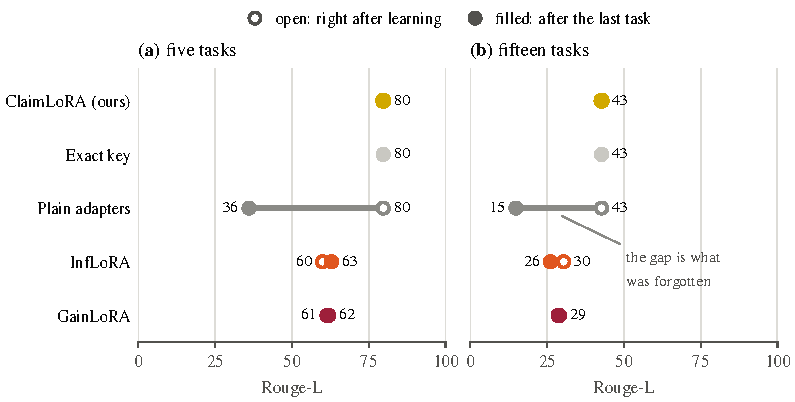
\includegraphics[width=0.9\linewidth]{figures/learn_forget}
  \caption{Learning and forgetting side by side, (a) on five tasks (mean over three seeds) and (b)
  on fifteen tasks (one seed). Open circle: average score of each task right
  after it was learned. Filled circle: average score after the last task. A gap between the two circles
  of a method is forgetting; an open circle far to the left is a lack of learning.}
  \label{fig:learnforget}
\end{figure}

Plain adapters learn and then forget (high open circle, low filled circle). On five tasks the two published methods have low and nearly equal circles: they forget little but learned less within ten epochs, so the comparison does not show that they forget, and we do not claim it. On fifteen tasks their open circles are low as well and the filled circles are lower for InfLoRA and, by less, for GainLoRA: some forgetting and a larger lack of learning, for reasons we did not separate (the method, the short budget, or our set-up). The certified switch has the open circle of plain adapters and no gap, since it leaves the training of an adapter untouched. The published results of both methods used 100 epochs and T5-large; we could not run that setting and the gap in learning may well close there. Without instructions the same two methods did forget more (Section~\ref{sec:nodefpublished}), with the same caveat on learning.

\subsection{What the zones add: a later task that looks like an old one}
\label{sec:stress}

On the benchmark sequences \nearest{} and \cert{} give the same routes, so they cannot show what the frozen zones and the priority of older tasks are for. They matter when a later task resembles an earlier one. A sixth task is added after the five tasks, with inputs of the same
kind as task~2 (SST-2 sentences) and a definition that is one of the rewordings of task~2's definition, as when someone adds ``the same task again'' with a different
instruction. Routes only, one constructed case. Table~\ref{tab:stress} counts how many of the
100 old test inputs of task~2 under each wording are routed differently afterwards.

\begin{table}[t]
  \caption{Stress test (T5-base word-vectors). A sixth task with SST-2 inputs and a
  reworded SST-2 definition is added after the five tasks. ``Blocked'': training
  inputs of the new task inside an older zone, reported when the task arrives. ``Routes
  changed'': old test inputs of task~2 (100 per wording) given to a different task
  afterwards.}
  \label{tab:stress}
  \centering
  \small
  \setlength{\tabcolsep}{4pt}
  \begin{tabular}{lccccccccc}
    \toprule
    & & \multicolumn{4}{c}{Routes changed, \cert{} $\downarrow$} & \multicolumn{4}{c}{Routes changed, \nearest{} $\downarrow$} \\
    \cmidrule(lr){3-6} \cmidrule(lr){7-10}
    New task's definition & Blocked & original & light & medium & heavy & original & light & medium & heavy \\
    \midrule
    light & 799 of 800 & 0 & 0 & 0 & 0 & 0 & 100 & 0 & 0 \\
    medium & 0 of 800 & 0 & 0 & 100 & 2 & 0 & 0 & 100 & 2 \\
    heavy & 0 of 800 & 0 & 0 & 0 & 100 & 0 & 0 & 0 & 100 \\
    \bottomrule
\end{tabular}

\end{table}

\paragraph{A look-alike inside an old zone is blocked and reported.} With the light rewording the inputs of the new task fall inside the zone of task~2: 799 of
its 800 training inputs are blocked, and the user is told when the task arrives, before any
training. Under \cert{} no old input changes its route. Under \nearest{} the old light-wording inputs carry the
instruction of the new task word for word and lie on its signature, so all 100 are
re-routed to it; the same text gets a different answer from then on, and nothing announces it. This is what the frozen zones are for: under the oldest-claim rule a certified input cannot be re-routed by a later task. Whether the old or the new task ought to answer such a text the rules do not
settle. Among \WidenTasksEval{} real tasks with machine-paraphrased instructions this was rare, and the zones did not prevent it there (Sections~\ref{sec:many}, \ref{sec:paraphrase}), so this constructed case is not typical of that collection.

\paragraph{A look-alike outside every zone can take uncertified inputs.} With the medium or heavy rewording the new signature lies outside the zone of task~2, nothing is
blocked, and under both rules the old inputs that carry exactly
that rewording are re-routed (100 of 100, plus 2 heavy-wording inputs in the medium case).
They were never certified; the certified inputs of task~2 (original and light wording) keep their route in every case. The guarantee protects exactly the certified inputs.

\subsection{What the zones cost: 875 real tasks}
\label{sec:many}

A large collection of real tasks contains look-alikes by itself. The \ManyTasks{} tasks of the default English split of Super-NaturalInstructions
\citep{wang2022superni} arrive in a random order, each with its definition and its first inputs (\ManyInputs{} inputs;
openings of \ManyOpeningMin{} to \ManyOpeningMax{} tokens, \ManyOpeningMedian{} in the middle; \ManyOpeningMax{} is the truncation length, so for these tasks the instance is cut off), and each gets its zone when it arrives. Routes only. The rules, including what would count against the method, were fixed
before the run (Appendix~\ref{app:many}).

\begin{table}[t]
  \caption{The zones on \ManyTasks{} real tasks in a random order (T5-base
  word-vectors, unedited instructions). ``Blocked'': inputs of a new task inside an older
  zone when it arrives; the columns count the tasks for which this holds for none, some or all
  of their inputs. ``Routes changed later'': inputs given to a different task
  than right after their own task arrived, under \cert{} / \exactfirst{} / \nearest{}.}
  \label{tab:many}
  \centering
  \small
  \setlength{\tabcolsep}{4pt}
  \begin{tabular}{rccccccc}
    \toprule
    & \multicolumn{3}{c}{Tasks with blocked inputs} & \multicolumn{3}{c}{Inputs to their own task, \%} & Routes \\
    \cmidrule(lr){2-4} \cmidrule(lr){5-7}
    Tasks & none & some & all & \cert{} & \exactfirst{} & \nearest{} & changed later \\
    \midrule
    50 & 49 & 1 & 0 & 98.7 & 100.0 & 100.0 & 0 / 0 / 0 \\
    100 & 96 & 3 & 1 & 96.7 & 100.0 & 100.0 & 0 / 0 / 0 \\
    200 & 178 & 7 & 15 & 90.4 & 99.0 & 98.5 & 0 / 0 / 0 \\
    400 & 337 & 13 & 50 & 85.7 & 99.2 & 99.0 & 0 / 0 / 0 \\
    875 & 724 & 22 & 129 & 83.8 & 98.4 & 98.3 & 0 / 0 / 0 \\
    \bottomrule
\end{tabular}

\end{table}

\begin{figure}[t]
  \centering
  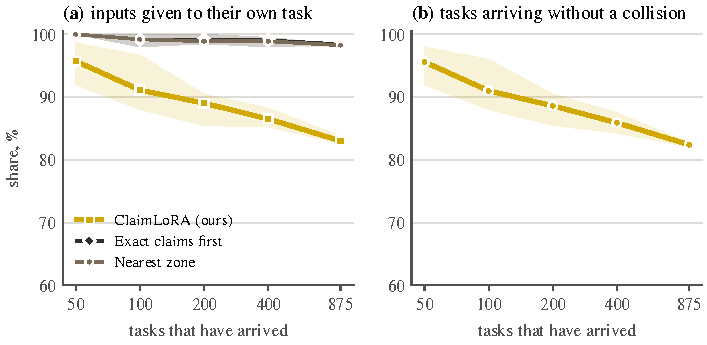
\includegraphics[width=0.86\linewidth]{figures/many}
  \caption{The price of the guarantee as the collection grows (same test as
  Table~\ref{tab:many}; means over five random orders, bands span the lowest
  and the highest). (a) Share of inputs given to their own task; the variant of
  Section~\ref{sec:exactfirst} and the nearest-zone rule nearly coincide. (b) Share of tasks that
  arrive with no input inside an older zone.}
  \label{fig:many}
\end{figure}

\paragraph{The guarantee holds, and its price grows with the collection.} No certified input changed
its route, in any order or at any size. But the larger the
collection, the more often a new task arrives inside an older zone (Figure~\ref{fig:many}). At the end \ManyColliding{} tasks
(\ManyCollidingPct{}\%) have collided with an older task, and for \ManyAllHeld{} every input is
blocked, so that under their given instruction they could not be learned. In four other
random orders \ManyCollidingPctLow{}\% to \ManyCollidingPctHigh{}\% collide,
and \ManyNumericCollidingPct{}\% in the order of the task numbers. These are not
accidents of the geometry: of the \ManyColliding{} colliding tasks, \ManySameText{} have the same
definition text as the task they collide with, \ManyAlikeHigh{} more share at least 80\% of its words,
and none shares less than \ManyAlikeLowest{}\%. They come from families
of tasks whose definitions differ in a word or two: \ManyFamilyMmlu{} are subject variants of one
multiple-choice task and \ManyFamilyAtomic{} relation variants of one classification task
(Table~\ref{tab:manyexamples}).

\paragraph{On unedited instructions the nearest-zone rule is the better rule.} \nearest{} gives
\ManyNearRightPct{}\% of the inputs to their own task and \cert{} \ManyCertRightPct{}\%, and neither re-routes an input later: an
input with an unedited instruction lies exactly on its task's signature, so no other zone can
be nearer. We had written down beforehand that \nearest{}
would re-route inputs here; that was wrong. The weakness of \nearest{} needs edited inputs (Section~\ref{sec:stress}).

\paragraph{The trade.} A zone protects a neighbourhood of an old instruction, where its light rewordings and fewer than half of its machine paraphrases lie, and takes it away from later tasks. Frozen zones block a later sibling and report the collision; a best-match rule serves the sibling and may re-route reworded inputs of the old task. With machine paraphrases of \WidenTasksEval{} real tasks (Section~\ref{sec:paraphrase}) the latter was rare and the zones did not reduce it:
\nearest{} changed \RerouteNearChanged{}\% of the routes (\RerouteNearNChanged{} of \RerouteInputs{}), the same \RerouteCertNChanged{} inputs as \cert{}; the plain nearest signature changed \RerouteSigChanged{}\% and gave more paraphrased inputs to their own task (\RerouteSigOwnEnd{}\% against \RerouteCertOwnEnd{}\%). Which event is more common depends on where a system is used; in a collection built from task
families, as this one is, it is the sibling. The radius factor moves the trade: with
$\kappa = 0.3$, \ManyCleanKappaThree{} of the \ManyTasks{} tasks arrive without a collision
instead of \ManyClean{} (Table~\ref{tab:manykappa}), but only 59\% of the lightly
reworded inputs of the five tasks are certified instead of all (Table~\ref{tab:kappa}). We
kept $\kappa = 0.5$, as fixed before this test.

\paragraph{A variant that serves the siblings.} \exactfirst{} (Section~\ref{sec:exactfirst}) was designed in response to this result, so its numbers on the same
collection are not an independent test. \ExactTasksOwn{} of the \ManyTasks{} tasks receive
all their own inputs when they arrive; the other \ExactTasksNone{} open token for token like an older
task. Nearly all inputs go to their own task in every order (\ExactRightPct{}\% at the end)
and none changes its route later (Table~\ref{tab:many}). In the stress test it serves the look-alike task, \ExactStressOwn{} of its
\StressTrain{} training inputs instead of \CertStressOwn{}, and pays as
Proposition~\ref{prop:exactfirst} says: the 100 old inputs that carry the look-alike's instruction
word for word are handed to it, and no other old input moves. Its routes are almost those of \nearest{}; what differs is what can be promised about an edited input
(Table~\ref{tab:guarantees}). No test separates the two on real inputs (on the French and German machine paraphrases they gave the same routes; on the Spanish ones \nearest{} gives \RerouteNearEsOwn{}\% and the variant \RerouteExactEsOwn{}\% to their own task), and the
variant has not been run with trained answers on a GPU.

\subsection{Mechanical edits of the instruction}
\label{sec:edits}

The instruction is damaged mechanically and the routes are looked at. Every test input of the fifteen tasks (1{,}197 inputs) gets
its own random edit of the task definition: $k$ words of at least four letters with a typo ($k$ capped at the number of such words; two neighbouring inner letters
swapped), $k$ words deleted, or $k$ words replaced by random words from the fifteen
definitions, for $k \in \{1, 2, 4, 8, 16\}$; the definition in lower case; the sentence ``Please
help me with this task.'' in front; the first or the last sentence of the
definition removed; or its sentences shuffled. That makes 23{,}640 edited inputs, routes only. The rules, including the outcomes that would count
against the method, were written into the repository before the run and nothing was changed
afterwards (Appendix~\ref{app:edits}). Line fixed before the run: a
share of inputs on their own task under 80\% for any edit counts against the method.

\begin{figure}[t]
  \centering
  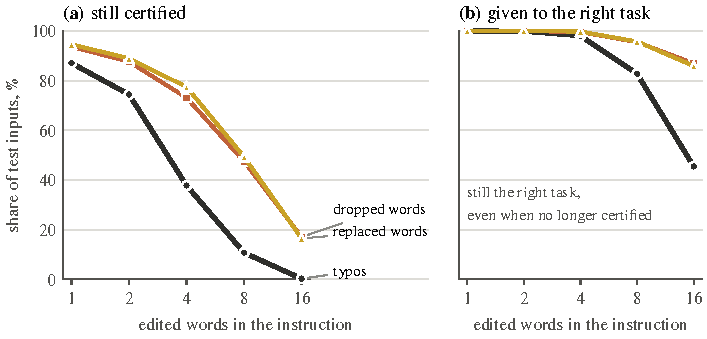
\includegraphics[width=0.86\linewidth]{figures/edits}
  \caption{Mechanical edits of the instruction, all fifteen tasks, routes only (1{,}197 test inputs per point, each with its own random edit). (a) Share of inputs
  still inside their own zone. (b) Share given to their own task.
  No edited input was inside the zone of another task.}
  \label{fig:edits}
\end{figure}

\begin{table}[t]
  \caption{Edits of the whole instruction (same test as Figure~\ref{fig:edits}). Tasks whose
  definition has a single sentence are left out of the last three rows.}
  \label{tab:edits}
  \centering
  \small
  \begin{tabular}{lccccc}
    \toprule
    Edit of the instruction & Tasks & Inputs & Certified inputs, \% & \shortstack[c]{Sent to own\\task, \% $\uparrow$} & Wrong zone \\
    \midrule
    Lower case & 15 & 1197 & 91.4 & 100.0 & 0 \\
    Sentence in front & 15 & 1197 & 91.6 & 100.0 & 0 \\
    First sentence removed & 14 & 1097 & 24.7 & 100.0 & 0 \\
    Last sentence removed & 14 & 1097 & 32.8 & 81.5 & 0 \\
    Sentences shuffled & 14 & 1097 & 100.0 & 100.0 & 0 \\
    \bottomrule
\end{tabular}

\end{table}

\paragraph{No edited input was certified for another task.} Not one of the 23{,}640 edited inputs
lay inside another task's zone; each was certified for its own task or not at all. This holds for these fifteen tasks, whose instructions are far apart; in the collection of Section~\ref{sec:many} inputs of sibling tasks do lie inside older
zones. A certificate promises that an answer stays the same, not that it comes from the right
task.

\paragraph{Small edits keep the certificate, large ones lose it.} With one typo 87.1\% of the inputs
are still certified, with one replaced word 94.6\%, with four edited words 38\% to 77\%, with sixteen
at most 17\% (Figure~\ref{fig:edits}a, Table~\ref{tab:edits}). A typo costs more than a dropped word (93.7\%), presumably because a misspelt word falls apart into
several rare word pieces, which carry a high weight in Eq.~\eqref{eq:weights}.

\paragraph{Heavy damage breaks the route of uncertified inputs.} Up to four edited
words at least 98.1\% of the inputs still reach their own task; with eight typos 82.7\%, with
sixteen typos 45.4\% (Figure~\ref{fig:edits}b). Verdict: the line is crossed, so under badly damaged instructions the nearest-zone route cannot be relied on. What the method offers is the missing certificate, which marks every one of these inputs.

\paragraph{Long instructions are robust, short ones are not.} Tasks whose opening has at least 90 tokens keep
98\% to 100\% of their inputs on the right task even with sixteen typos (Table~\ref{tab:editspertask}). The two tasks that fail
first have the shortest instructions: \texttt{sciq} (ten words, opening of 26
tokens) and \texttt{xsum} (34 tokens); with eight typos only 3\% and 18\% of their inputs arrive. With sixteen typos every word of four or more letters in a definition of ten words carries a typo.

\paragraph{Two findings that follow from how the switch reads.} Removing the last sentence of the
definition leaves 81.5\% of the inputs on their task, but only 2\% for SST-2 and 8\% for emotion
classification, where that sentence states the task. Shuffling the
sentences changes nothing and every input stays certified, because the feature of
Eq.~\eqref{eq:prefix} is an average and ignores word order
(Proposition~\ref{prop:edits}).

\paragraph{The guaranteed tolerance.} The largest distance between two rows of the rescaled
embedding table of T5-base is $D = 509.6$, and the ratio $R_k / D$ of Proposition~\ref{prop:edits}
lies between 2.0\% and 4.2\% for the fifteen tasks. Edits that remove at most this share of the
weight of the opening, and add at most this share, can never leave the zone; in tokens of average weight this is the replacement of \BoundTokensLow{} to \BoundTokensHigh{} tokens,
depending on the task. The measured tolerance is far larger, as it must be, since the bound has to
cover the two most different tokens of the vocabulary. On \BoundInputs{} edited inputs (ten per task and edit with
typos, dropped and replaced words) the bound held for every one: the inputs moved by at most
\BoundWorstPct{}\% of what it allows, \BoundMedianPct{}\% in the middle, and the bound
alone would have certified \BoundGuaranteed{} of the \BoundInside{} inputs that stayed inside
their zone.

\subsection{The order of the tasks}
\label{sec:orders}

The signature of a task depends on its own opening only, and its radius on the signatures known
when it arrives, so the routes under any other order of arrival can be computed exactly without training. Table~\ref{tab:orders} gives them for all
120 orders of the five tasks, the two official orders of the benchmark and 1{,}000 random
orders of the fifteen tasks.

\begin{table}[t]
  \caption{The order of the tasks (routes only, T5-base word-vectors). Entries with four numbers are
  for the original / light / medium / heavy wording; the reworded inputs are those of the five tasks.
  ``Blocked'': training inputs inside an older zone. ``Changed'': test inputs whose route changed
  after their task had been added; a range depends on the order.}
  \label{tab:orders}
  \centering
  \footnotesize
  \setlength{\tabcolsep}{3.5pt}
  \begin{tabular}{lcccccc}
    \toprule
    Sequence & Orders & \shortstack[c]{Sent to own\\task, \% $\uparrow$} & \shortstack[c]{Certified\\inputs, \%} & Wrong zone & Blocked & \shortstack[c]{Routes\\changed $\downarrow$} \\
    \midrule
    5 tasks, all orders & 120 & 100/100/100/93.8 & 100/100/20/19.6 & 0 & 0 & 0--31 \\
    \midrule
    15 tasks, official order 1 & 1 & 100/100/100/93.8 & 100/100/20/19.6 & 0 & 0 & 0 \\
    15 tasks, official order 2 & 1 & 100/100/100/93.8 & 100/100/20/19.6 & 0 & 0 & 31 \\
    15 tasks, random orders & 1,000 & 100/100/100/93.8 & 100/100/20/19.6 & 0 & 0 & 0--31 \\
    \bottomrule
\end{tabular}

\end{table}

In every order all inputs with the original wording are certified, none lies in a foreign
zone, no training input is blocked, and the shares reaching their own task are the
same to the last digit. For 13 of the 15 tasks the nearest known signature is
that of an unrelated task, known from the start, so their radius does not depend on the order (Table~\ref{tab:distances}). The two exceptions are \texttt{samsum} and \texttt{xsum}, whose nearest signature is that of a third summarisation task
(\texttt{reddit\_tifu}); their radius is up to 7\% and 13\% smaller if it was learned
before them, and no test input is affected.

The order decides \emph{when} an uncertified input goes wrong. The 31 heavily
reworded tweets given to SST-2 go to it from the start if SST-2 is learned before
Sentiment140 (our five-task sequence, official order~1). If SST-2 comes later (official
order~2), they first go to their own task and are re-routed when SST-2
arrives: 31 routes change after the inputs were first answered, and with a route the answer
changes in general. They are uncertified, and
Proposition~\ref{prop:uncertified} says this can happen; for certified inputs it cannot.

\subsection{The unrelated inputs}
\label{sec:background}

The collection $\mathcal{B}$ of unrelated inputs sets the token
weights, the scale of distances, and the signatures of the unrelated tasks, which fix most radii. To see whether the results depend on this collection, the route
computations were repeated with two other random draws of the 4{,}000 inputs, with 500, 1{,}000 and 2{,}000 inputs,
and with only five of the ten unrelated tasks in two ways (Table~\ref{tab:background}; the settings and what would count against the method were fixed beforehand, routes only). In
all eight settings every input with the original or the light wording is certified, every input
with the original, light or medium wording reaches its own task, none lies in a foreign zone,
and no training input is blocked: the part of the results that rests on the guarantee did not depend on the choice. The share of heavily reworded inputs that reach their own task did,
from \BackgroundHeavyLow{}\% to \BackgroundHeavyHigh{}\%, so the 93.8\% of the main configuration is one draw from that range and not a property of the method.
We had expected the radii to change with only five unrelated tasks; they hardly did, and at most two more heavily reworded inputs were certified.

\subsection{Other models}
\label{sec:models}

\paragraph{The routes with other embedding tables.} The switch needs only a tokenizer and an embedding table, so the routes can be computed without training for any
model. Table~\ref{tab:models} does this for eight models: T5 in three sizes \citep{raffel2020t5} and Flan-T5
\citep{chung2024flant5}, GPT-2 \citep{radford2019gpt2}, SmolLM2
\citep{allal2025smollm2}, Qwen2.5 \citep{yang2024qwen25} and RoBERTa
\citep{liu2019roberta}, with embedding dimensions from 512 to 1024 and five different
vocabularies. Nothing was adjusted per model; the radius factor and word weights are those of
Section~\ref{sec:method}. Routes only. For every model, every test input with the original wording lies in its
own zone in the five-task and the 15-task sequence, none lies in a foreign zone, and no
training input of a later task is blocked. With light rewording 99\% to 100\% of the inputs are
certified and with medium rewording all reach their own task. Models differ under heavy rewording: 80\% to 99\% reach their own task, and the routes of three uncertified inputs changed when a later task arrived (two with Flan-T5, one with GPT-2); no certified route changed.

\begin{table}[t]
  \caption{Routes computed with the embedding tables of eight models (CPU, no training). Entries
  with four numbers are for the original / light / medium / heavy wording. ``Wrong zone'': inputs
  inside the zone of another task, over both sequences and all wordings. ``Changed'': inputs
  whose route changed after their task had been added. With the original wording every input of
  the 15-task sequence is certified for every model.}
  \label{tab:models}
  \centering
  \footnotesize
  \setlength{\tabcolsep}{3pt}
  \begin{tabular}{lcccccc}
    \toprule
    & & \multicolumn{2}{c}{Five tasks} & Fifteen tasks & & \\
    \cmidrule(lr){3-4} \cmidrule(lr){5-5}
    Embedding table of & \shortstack[c]{Embedding\\dimension\\$d$} & \shortstack[c]{certified\\inputs, \%} & \shortstack[c]{sent to\\own task,\\\% $\uparrow$} & \shortstack[c]{sent to\\own task,\\\% $\uparrow$} & Wrong zone & \shortstack[c]{Routes\\changed\\$\downarrow$} \\
    \midrule
    \texttt{t5-small} & 512 & 100/100/20/20 & 100/100/100/89 & 100/100/100/89 & 0 & 0 \\
    \texttt{t5-base} & 768 & 100/100/20/20 & 100/100/100/94 & 100/100/100/94 & 0 & 0 \\
    \texttt{t5-large} & 1024 & 100/100/20/19 & 100/100/100/83 & 100/100/100/83 & 0 & 0 \\
    \texttt{flan-t5-base} & 768 & 100/100/20/14 & 100/100/100/99 & 100/100/100/99 & 0 & 2 \\
    \texttt{gpt2} & 768 & 100/99/20/20 & 100/100/100/87 & 100/100/100/87 & 0 & 1 \\
    \texttt{SmolLM2-135M} & 576 & 100/99/20/20 & 100/100/100/82 & 100/100/100/82 & 0 & 0 \\
    \texttt{Qwen2.5-0.5B} & 896 & 100/99/20/20 & 100/100/100/80 & 100/100/100/80 & 0 & 0 \\
    \texttt{roberta-base} & 768 & 100/99/20/20 & 100/100/100/94 & 100/100/100/93 & 0 & 0 \\
    \bottomrule
\end{tabular}

\end{table}

\paragraph{Training other models with the stand-alone code.} The stand-alone implementation
(Appendix~\ref{app:impl}) was run on T5-small, GPT-2 and
SmolLM2-135M on a CPU: five tasks, 400 training
examples and five epochs each, 30 to 50 test inputs per task, one seed. The runs are small on purpose: they show whether the code
keeps answers on another architecture, not how good these models can become. In all three (Table~\ref{tab:demo}) the certified switch ends exactly where it stood right after learning, no
answer of an earlier task changes, and every test input with the original wording is certified. With
all adapters on, the same adapters end far lower and nearly all answers of earlier tasks change. With heavily reworded instructions no answer changes either, and
\DemoTfiveHeavyRight{}\%, \DemoGptHeavyRight{}\% and \DemoSmolHeavyRight{}\% of those inputs reach
their own task.

\begin{table}[t]
  \caption{The stand-alone implementation on three small models (CPU, five tasks, 400 training
  examples and 5 epochs per task, one seed). ``Changed'': answers of the first four tasks that
  differ at the end. ``Certified'': test inputs with the original wording inside a zone.
  ``enc.-dec.'': encoder-decoder; ``dec.-only'': decoder-only.}
  \label{tab:demo}
  \centering
  \footnotesize
  \setlength{\tabcolsep}{3pt}
  \begin{tabular}{llcccccccc}
    \toprule
    & & \multicolumn{3}{c}{\cert{}, original} & \multicolumn{2}{c}{\plain{}, original} & & \multicolumn{2}{c}{\cert{}, heavy} \\
    \cmidrule(lr){3-5} \cmidrule(lr){6-7} \cmidrule(lr){9-10}
    Model & Kind & \shortstack[c]{Score\\right\\after\\learning\\$\uparrow$} & \shortstack[c]{Final\\score\\$\uparrow$} & \shortstack[c]{Answers\\changed $\downarrow$} & \shortstack[c]{Final\\score\\$\uparrow$} & \shortstack[c]{Answers\\changed $\downarrow$} & \shortstack[c]{Certified\\inputs} & \shortstack[c]{Final\\score\\$\uparrow$} & \shortstack[c]{Answers\\changed $\downarrow$} \\
    \midrule
    \texttt{SmolLM2-135M} & dec.-only & 74.3 & 74.3 & 0 of 120 & 27.7 & 100 of 120 & 150 of 150 & 65.1 & 0 of 120 \\
    \texttt{gpt2} & dec.-only & 67.9 & 67.9 & 0 of 120 & 15.8 & 119 of 120 & 150 of 150 & 54.8 & 0 of 120 \\
    \texttt{t5-small} & enc.-dec. & 65.8 & 65.8 & 0 of 200 & 12.0 & 200 of 200 & 250 of 250 & 56.2 & 0 of 200 \\
    \bottomrule
\end{tabular}

\end{table}

\paragraph{A sibling task, with trained answers.} \exactfirst{} was also run with the
stand-alone code on T5-small. After the five tasks a sixth is learned: the sentences of SST-2
under the lightly reworded SST-2 definition, with other answer words (``good'' and ``bad''
instead of ``POS'' and ``NEG'') so that one can see which adapters answered, learned
twice from the same starting point. Under \cert{} all \SiblingCertBlocked{} of its
\SiblingTrain{} training inputs are blocked; its test inputs are still answered in
the words of the old task (\SiblingCertRight{} of \SiblingTest{} right), and no answer of the five
old tasks changes in any wording. Under \exactfirst{} the task is learned (\SiblingExactRight{} of
\SiblingTest{} right), no answer to an unedited input of the old tasks changes, and the
\SiblingExactChangedLight{} old SST-2 test inputs that carry the sibling's instruction word for
word now get the sibling's answer; nothing else changes (\SiblingOldInputs{} old test inputs per
wording). This is one small model and one constructed sibling, not a test of the variant at scale.

\subsection{Rewording at scale: machine paraphrases of 700 real tasks}
\label{sec:paraphrase}

The definitions of the \WidenTasksAll{} real tasks of Section~\ref{sec:many} were paraphrased by machine: back-translation through German and through French, sentence by sentence, with MarianMT models \citep{junczys2018marian,tiedemann2020opusmt} and beam search without sampling. On average \WidenKeptDe{}\% (German) and \WidenKeptFr{}\% (French) of the words of a definition survive; \WidenSameDe{} German and \WidenSameFr{} French paraphrases equal the original. Spanish and Italian pivots were made later, for the checks below (\WidenSpKept{}\% and \RerouteItKept{}\% of the words survive; \WidenSpSame{} and \RerouteItSame{} paraphrases equal the original). All paraphrases are used as they come. A paraphrased input is an input of its task with its definition replaced by the paraphrase. \WidenTasksCal{} tasks are kept for choosing and calibrating (not used again), \WidenTasksEval{} are used for evaluation in a random order of arrival, each with its zone. Nothing is trained: the tests compute routes only, with the T5-base word-vectors and the rule of Section~\ref{sec:method} unchanged. The tasks come from one collection, many of them are siblings, and the paraphrases are made by translation models, not by people; one split and one order of arrival are used except where stated.

\paragraph{Measures.} All are shares. \textsf{C}: tasks that arrive with at least one unedited input inside an older zone. \textsf{U}: unedited inputs given to their own task. \textsf{P}: paraphrased inputs inside their own task's zone and given to it (a correct certificate). \textsf{M}: paraphrased inputs certified for \emph{another} task (a wrong certificate: the answer is stable but comes from the wrong adapters). \textsf{R}: paraphrased inputs given to their own task, with or without a certificate. The letters name measures in this section and its appendix only; they are not the covariance, the radius or the zone of the method.

\paragraph{Result for \cert{}.} Tables~\ref{tab:widenmain} and~\ref{tab:widenspanish} give the numbers by pivot. With \WidenParaInputs{} paraphrased inputs (German and French together) \textsf{C}~=~\WidenRefTfiveC{}\%, \textsf{U}~=~\WidenRefTfiveU{}\%, \textsf{P}~=~\WidenRefTfiveP{}\%, \textsf{M}~=~\WidenRefTfiveM{}\% and \textsf{R}~=~\WidenRefTfiveR{}\%; across the pivots \textsf{P} runs from \WidenRefTfivePLow{}\% to \WidenRefTfivePHigh{}\%. On the Italian pivot (not in these tables) \textsf{P}~=~\WidenRefTfiveItP{}\%, \textsf{M}~=~\WidenRefTfiveItM{}\% and \textsf{R}~=~\WidenRefTfiveItR{}\%, in the same ranges. \cert{} was not tuned on any pivot. So between four and five in ten paraphrased inputs get a correct certificate, at most about one in ten a wrong one, the rest none, and about three quarters reach their own task. The \FiveCertRightLight{}\%, \FiveCertRightMedium{}\% and \FiveCertRightHeavy{}\% of Section~\ref{sec:reworded} were measured on five tasks far apart with the development rewordings. This is a limitation of the method as built: the zones are narrow at scale.

\paragraph{Can the zones be made wider?} Five attempts, each with a line fixed before the run (set-ups and numbers in Appendix~\ref{app:widen}; Table~\ref{tab:widenmain}, Figure~\ref{fig:widen}). None met its line.
(1) Hidden states of a frozen causal language model instead of word-vectors: line, 20 points more correct certificates at no higher collision rate and no more wrong certificates; verdict, against (wrong certificates rose).
(2) A metric in units of what paraphrasing does: line, 20 points more \textsf{P} at equal \textsf{C} with no more \textsf{M}; verdict, against.
(3) A frozen sentence encoder \citep{reimers2019sbert,wang2020minilm} with a split-conformal radius.
(4) A zone decided by a frozen inference model \citep{he2023debertav3} that judges whether two instructions ask for the same thing.
(5) The same judge, sentence by sentence.
For (3) to (5) the line was \textsf{P}~$\ge$~75\%, \textsf{M}~$\le$~5\% and \textsf{C}~$\le$~19\% (against: \textsf{P}~$<$~55\%, \textsf{M}~$>$~9\% or \textsf{C}~$>$~25\%), read on the French pivot for (3) and (4) and on the Italian pivot, which no study had read, for (5). Verdict: against for all three. (3) and (5) lift \textsf{P} but \textsf{M} stays above 9\% ((5), with \textsf{P} and \textsf{C} on the right side of the success lines, is the best point so far); (4) has far more wrong certificates and collisions (\textsf{M} far above 9\%, \textsf{C} above 25\%, \textsf{P} below 75\%; Table~\ref{tab:widenmain}). Most colliding tasks are siblings that differ in one or a few decisive words (a date format day-month against month-day, the closest integers against the farthest, a person's reaction against their intent in the ATOMIC tasks; Table~\ref{tab:widensiblings}), and every feature tried puts their rewordings together.

\begin{table}[t]
  \caption{Machine paraphrases of 700 real tasks, routes only: \cert{} and the attempts to widen the zones, in the setting named before each run. \textsf{C}, \textsf{P}, \textsf{M}, \textsf{R} in \%. ``Both'': German and French pivot together (\WidenParaInputs{} inputs); French rows \WidenParaInputsPivot{} inputs, except (4) and (5), which count one paraphrased instruction per task (\WidenTasksEval{}) and whose \textsf{C} is about the original instructions. Paper: T5-base word-vectors, $\kappa = 0.5$; its French row is the reference for (2) to (4). (1): SmolLM2-135M, last layer, one radius, own reference row. (2): metric fitted on paraphrases, read at the radius where \textsf{C} equals that of \cert{}; the pre-registered reference is the old ruler at that radius (\textsf{P} \WidenRulerTfivePOld{}\%, \textsf{M} \WidenRulerTfiveMOld{}\%). (3): MiniLM-L6, paraphrase ruler, $\alpha = 0.1$. (4): MiniLM filter and DeBERTa-v3-xsmall judge, $\tau = \WidenJudgeTau{}$. (5): the same judge sentence by sentence, Italian pivot.}
  \label{tab:widenmain}
  \centering
  \footnotesize
  \setlength{\tabcolsep}{3pt}
  \begin{tabular}{llcrrrrl}
    \toprule
    & Features and zone & Pivot & \textsf{C} & \textsf{P} & \textsf{M} & \textsf{R} & Verdict \\
    \midrule
    Paper & T5-base word-vectors, weighted mean & both & 16.9 & 40.5 & 7.6 & 75.4 & reference \\
    Paper & T5-base word-vectors, weighted mean & French & 16.9 & 39.8 & 9.2 & 75.4 & ref. for (2)--(4) \\
    \midrule
    (1) & SmolLM2 word-vectors & both & 18.9 & 42.1 & 8.9 & 75.6 & ref. for (1) \\
    (1) & SmolLM2 last layer & both & 25.7 & 64.9 & 13.7 & 83.2 & against \\
    (2) & T5-base, paraphrase ruler & French & 16.9 & 42.0 & 10.7 & 84.4 & against \\
    (3) & MiniLM, ruler, $\alpha = 0.1$ & French & 16.6 & 71.2 & 11.6 & 86.1 & against \\
    (4) & MiniLM and NLI judge & French & 36.0 & 58.9 & 34.7 & 64.7 & against \\
    (5) & MiniLM, sentence-wise NLI judge & Italian & 12.4 & 76.1 & 10.9 & 88.7 & against \\
    \midrule
    Bar (3)--(5) & \multicolumn{2}{l}{fixed in advance} & $\le 19$ & $\ge 75$ & $\le 5$ & & \\
    \bottomrule
\end{tabular}

\end{table}

\begin{figure}[t]
  \centering
  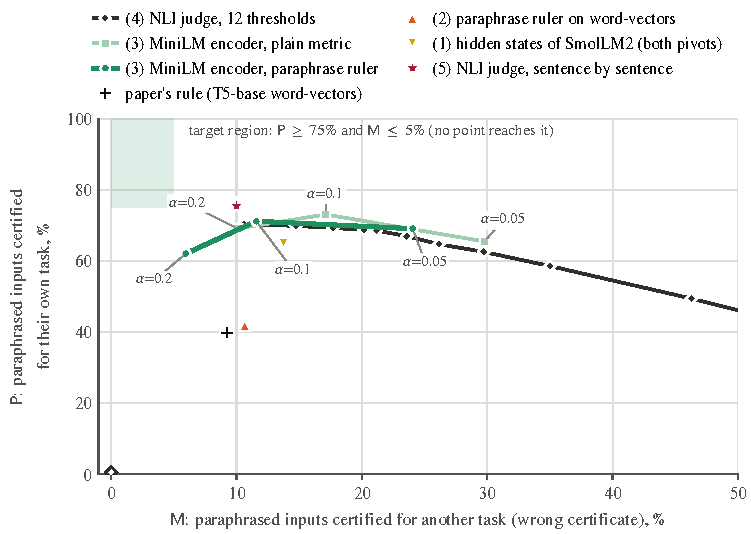
\includegraphics[width=0.86\linewidth]{figures/widen_tradeoff}
  \caption{Correct against wrong certificates on paraphrased inputs (French pivot; (1): both pivots). The shaded box is the target. The sentence encoder (3) is shown plain and with the ruler at $\alpha = 0.05, 0.1, 0.2$; the judge (4) has one point per threshold (the strictest, open, covers almost nothing; the loosest lies beyond the right edge). Only (3) at $\alpha = 0.1$, (4) at $\tau = \WidenJudgeTau{}$ and (5), at its French-pivot value, were named before the runs.}
  \label{fig:widen}
\end{figure}

\paragraph{A setting looked at after the runs.} The encoder with the ruler at $\alpha = 0.2$, not the primary setting, was ahead of \cert{} on every measure on the French pivot. Line fixed before the run: on Spanish-pivot paraphrases, which no study had read, with nothing fitted again, it gains at least \WidenSpAskP{} points in \textsf{P} and \WidenSpAskR{} in \textsf{R} with no more wrong certificates. Verdict: not confirmed (Table~\ref{tab:widenspanish}); the gain in \textsf{P} is \WidenSpGainP{} points, the gain in \textsf{R} (\WidenSpGainR{}) and \textsf{M} pass. On \WidenSplitCount{} other random splits (Table~\ref{tab:widensplits}) the encoder setting has more wrong certificates than \cert{} on \WidenSplitMoreM{} and more collisions on \WidenSplitMoreC{}: the advantage belongs to the original split. We report the encoder zone as a variant, not as an improvement. Its costs and the remaining numbers are in Appendix~\ref{app:widen}.

\begin{table}[t]
  \caption{Spanish-pivot check: \cert{} and the encoder setting (paraphrase ruler, $\alpha = 0.2$) on three pivots, \WidenSpInputs{} paraphrased inputs each; nothing fitted again for Spanish. In \%.}
  \label{tab:widenspanish}
  \centering
  \footnotesize
  \setlength{\tabcolsep}{3pt}
  \begin{tabular}{lrrrrrrrrrr}
    \toprule
    & & \multicolumn{3}{c}{French} & \multicolumn{3}{c}{German} & \multicolumn{3}{c}{Spanish} \\
    \cmidrule(lr){3-5} \cmidrule(lr){6-8} \cmidrule(lr){9-11}
    & \textsf{C} & \textsf{P} & \textsf{M} & \textsf{R} & \textsf{P} & \textsf{M} & \textsf{R} & \textsf{P} & \textsf{M} & \textsf{R} \\
    \midrule
    Paper's rule & 16.9 & 39.8 & 9.2 & 75.4 & 41.2 & 5.9 & 75.5 & 50.4 & 9.7 & 77.5 \\
    Encoder & 12.1 & 62.1 & 6.0 & 90.0 & 72.6 & 8.1 & 89.7 & 63.8 & 5.3 & 91.7 \\
    \bottomrule
\end{tabular}

\end{table}

\begin{table}[t]
  \caption{The same two rules on \WidenSplitCount{} other random splits of the \WidenTasksAll{} tasks, Spanish pivot: mean (smallest to largest), ruler and radius fitted again on each split. In \%.}
  \label{tab:widensplits}
  \centering
  \footnotesize
  \begin{tabular}{lcc}
    \toprule
    Spanish pivot & Paper's rule & Encoder \\
    \midrule
    Tasks that collide (\textsf{C}), \% $\downarrow$ & 16.0 (14.3 to 17.3) & 12.7 (9.1 to 16.6) \\
    Right certificate (\textsf{P}), \% $\uparrow$ & 49.4 (48.3 to 50.7) & 63.1 (55.5 to 70.0) \\
    Wrong certificate (\textsf{M}), \% $\downarrow$ & 7.9 (4.2 to 10.4) & 6.0 (2.4 to 9.7) \\
    Sent to own task (\textsf{R}), \% $\uparrow$ & 76.9 (75.8 to 78.1) & 90.4 (87.7 to 93.3) \\
    \bottomrule
\end{tabular}

\end{table}

\paragraph{Do later tasks re-route reworded inputs?} The paraphrased inputs show how often, among real tasks, a best-match rule changes an old route (Section~\ref{sec:stress} built such a case by hand). Each input's route right after its own task has arrived is compared with its route after all \WidenTasksEval{} tasks. Line fixed before the run (Appendix~\ref{app:reroute}): the zones add something at scale if \nearest{} changes at least 5\% of the routes and \cert{} at most half as many, and little if \nearest{} changes fewer than \RerouteLimitLow{}\%. Verdict: ``the zones add little here'' (Table~\ref{tab:reroute}). \nearest{} changed \RerouteNearNChanged{} of \RerouteInputs{} routes and \cert{} the same \RerouteCertNChanged{}, all outside every zone; none of the \RerouteCertInZone{}\% of inputs inside a zone at arrival changed, as Theorem~\ref{thm:writeonce} says, and the nearest-zone rule did not change them either. We had expected \RerouteExpectNearLow{}\% to \RerouteExpectNearHigh{}\% for \nearest{}; that was wrong. Here the certified switch adds the proof and no stability that we could measure.

\begin{table}[t]
  \caption{Do later tasks re-route reworded inputs? Routes only; \WidenTasksEval{} real tasks. ``Own'': share of the \RerouteInputs{} paraphrased inputs (French and German pivot) given to their own task after all tasks; ``Italian: own'': the same on the \RerouteInputsPivot{} Italian-pivot inputs. ``Changed'': route after all tasks differs from the route right after the input's own task arrived. ``In a zone'': inside a zone at arrival. ``Unedited'': unedited inputs given to their own task at the end (none changed under any rule). \signature{}: nearest signature in plain distance. \hybrid{}: oldest zone that holds the input, else \signature{}. \scaled{}: nearest signature with its distance divided by the distance of the task's signature to the nearest signature of the unrelated tasks. \certscaled{}: oldest zone that holds the input, else \scaled{}. \hybrid{} and \scaled{} were designed after the earlier results were seen, on the same data; none has a free setting.}
  \label{tab:reroute}
  \centering
  \scriptsize
  \setlength{\tabcolsep}{2pt}
  \begin{tabular}{lrrrrr}
    \toprule
    Rule & \shortstack[r]{Sent to own\\task, \% $\uparrow$} & \shortstack[r]{Italian pivot: sent\\to own task, \% $\uparrow$} & \shortstack[r]{Routes changed,\\\% (n) $\downarrow$} & \shortstack[r]{Inside a zone\\at arrival, \%} & \shortstack[r]{Unedited, sent to\\own task, \% $\uparrow$} \\
    \midrule
    \signature{} (plain nearest signature) & 91.3 & 93.1 & 2.22 (93) & -- & 98.4 \\
    \nearest{} (nearest zone) & 75.4 & 77.0 & 0.31 (13) & -- & 98.4 \\
    \cert{} (the rule of the paper) & 75.4 & 76.8 & 0.31 (13) & 48.1 & 83.1 \\
    \hybrid{} (zones, then nearest signature) & 85.6 & 88.5 & 1.95 (82) & 48.1 & 83.1 \\
    \scaled{} (scaled by the distance to unrelated text) & 94.4 & 95.9 & 1.60 (67) & -- & 98.4 \\
    \certscaled{} (zones, then \scaled{}) & 88.6 & 91.3 & 1.33 (56) & 48.1 & 83.1 \\
    \bottomrule
\end{tabular}

\end{table}

\begin{table}[t]
  \caption{The same rules on the benchmark tasks with the development rewordings (routes only): share of the \RerouteBenchInputs{} inputs given to their own task after the last task; ``(n)'': routes changed by later tasks (of \RerouteBenchInputs{}, including the inputs of the last task, which cannot change). With the original and the light wording every rule gives 100\% and changes nothing.}
  \label{tab:reroutebench}
  \centering
  \footnotesize
  \setlength{\tabcolsep}{3pt}
  \begin{tabular}{lrrrr}
    \toprule
    & \multicolumn{2}{c}{Five tasks} & \multicolumn{2}{c}{Fifteen tasks} \\
    \cmidrule(lr){2-3} \cmidrule(lr){4-5}
    Rule & \shortstack[r]{Medium wording:\\own task, \% $\uparrow$\\(routes changed)} & \shortstack[r]{Heavy wording:\\own task, \% $\uparrow$\\(routes changed)} & \shortstack[r]{Medium wording:\\own task, \% $\uparrow$\\(routes changed)} & \shortstack[r]{Heavy wording:\\own task, \% $\uparrow$\\(routes changed)} \\
    \midrule
    \signature{} & 76.8 (55) & 60.0 (100) & 71.6 (74) & 60.0 (100) \\
    \nearest{} & 100.0 (0) & 93.8 (0) & 100.0 (0) & 93.8 (0) \\
    \cert{} & 100.0 (0) & 93.8 (0) & 100.0 (0) & 93.8 (0) \\
    \hybrid{} & 76.8 (55) & 60.0 (100) & 71.6 (74) & 60.0 (100) \\
    \scaled{} & 100.0 (0) & 93.8 (0) & 100.0 (0) & 93.8 (0) \\
    \certscaled{} & 100.0 (0) & 93.8 (0) & 100.0 (0) & 93.8 (0) \\
    \bottomrule
\end{tabular}

\end{table}

Two more rules were added after this result, each with its reading fixed before it was computed (details in Appendix~\ref{app:reroute}). The plain nearest signature changed \RerouteSigNChanged{} routes (``some'', below the 5\% expected) but gave \RerouteSigOwnEnd{}\% of paraphrased inputs to their own task against \RerouteCertOwnEnd{}\% for \cert{} and \nearest{}: at this scale the simplest rule serves reworded inputs better and pays with about two silent changes in a hundred. Dividing the distance by the radius, the fallback of \cert{} chosen on the benchmark tasks, keeps routes stable here and gives fewer inputs to their own task. \hybrid{} (zones, then the plain signature; designed after that result, on the same data) keeps every certificate and gives \RerouteHybOwnEnd{}\% to their own task with \RerouteHybChanged{}\% changed routes, but on the benchmark with heavy rewording far fewer than \cert{} (\RerouteHybBenchFiveHeavyOwn{}\% against \RerouteCertBenchFiveHeavyOwn{}\%; Table~\ref{tab:reroutebench}). The two fallbacks trade places between the tests, so \hybrid{} is not a repair.

Why (read from the numbers, not tested): the radius of a zone is half the distance to the nearest known signature, unrelated or earlier. With $U_k$ the distance to the nearest unrelated signature, the radius is half of $U_k$ for all five benchmark tasks and \RerouteBBenchFifteenCount{} of fifteen, but for only \RerouteBShare{}\% of the \WidenTasksEval{} real tasks; for the others an earlier sibling is nearer, the newer sibling's radius is tiny and its reworded inputs are turned away.

Two fallbacks were tested for this. Line fixed before the run, verdict at scale read on a fourth pivot, Italian, that no study had read: at least \RerouteLineHeavy{}\% of inputs to their own task under heavy and \RerouteLineMedium{}\% under medium rewording on the benchmark (five and fifteen tasks) and at least \RerouteLineItalian{}\% on Italian; heavy below \RerouteLineHeavyAgainst{}\% or Italian below \RerouteLineItalianAgainst{}\% counts against. Verdict: scaling by the length of the opening failed (\RerouteNormHeavyFive{}\% under heavy rewording, although \RerouteNormItOwn{}\% on Italian); scaling by $U_k$ alone, \scaled{}, succeeded: on the benchmark it equals \cert{} under heavy and medium rewording (Table~\ref{tab:reroutebench}), and on the real tasks it gives \RerouteBgItOwn{}\% (Italian) and \RerouteBgOwnEnd{}\% (French and German) to their own task (Table~\ref{tab:reroute}). With the zones in front (\certscaled{}: same certificates, same theorem) it gives \RerouteCertFourOwnEnd{}\%, where \cert{} gives \RerouteCertOwnEnd{}\%, and the benchmark routes are those of \cert{}, input by input at every scored point (\RerouteIdFiveLast{} differing routes in \RerouteIdFiveComparisons{} comparisons on five tasks; fifteen tasks: \RerouteIdFifteenLast{} after the last task, \RerouteIdFifteenScored{} at any scored point), so every GPU score of \cert{} and \nearest{} is also the score of the variant. Limits of this variant, found at the end of the work: it changes more routes after arrival than \cert{} (Table~\ref{tab:reroute}); in the stress test of Section~\ref{sec:stress} a look-alike with the light rewording as its definition takes \RerouteStressCertFourMedium{} (medium) and \RerouteStressCertFourHeavy{} (heavy) of \RerouteStressOld{} uncertified old inputs that \cert{} kept, and one with the medium rewording takes \RerouteStressMedCertFourHeavy{} heavy ones, where \cert{} loses \RerouteStressMedCertHeavy{}; no certified input changes; the zones cost \RerouteZonesCost{} points of right routes on Italian, \RerouteZonesCostFG{} on French and German and \RerouteZonesCostEs{} on Spanish against the best rule without zones and give a proof for about half of the inputs (\RerouteCertInZone{}\% at arrival). The benchmark rewordings are the development set, no GPU run was repeated with it, no rule here was run with trained answers, and \cert{} stays the zone rule of every GPU run with instructions.

\paragraph{The guarantee does not depend on the zone.} Theorem~\ref{thm:writeonce} needs only that the zone is a fixed set once its task has arrived and that membership is computed reproducibly from frozen parts (Remark~\ref{rem:otherzones}). It holds for every zone here as defined; for the judge zone as measured, which judges only the \WidenJudgeLimit{} nearest tasks, see Appendix~\ref{app:widen}. A certificate promises a stable answer, not the right task. The edit bound of Proposition~\ref{prop:edits} does not carry over, because it needs an average. The development rewordings of the five benchmark tasks move further than a back-translation: with the sentence encoder \WidenEncBenchMediumZone{}\% (medium) and \WidenEncBenchHeavyZone{}\% (heavy) of them lie inside their own zone, all still go to the right task.

\subsection{Zones from the inputs of a task: the first test without instructions}
\label{sec:noinstruction}

This is the first test of the rule of Section~\ref{sec:bound} (Theorem~\ref{thm:bound}): a zone built from the inputs of the task itself, sized on held-out inputs, so that for any model and any later tasks each input of the task changes its answer with probability at most a chosen level. It was run before the recogniser of Section~\ref{sec:recogniser} existed, and its two findings (blocked tasks, the need for a better feature) are why that recogniser was built. Pilot A computes routes only, on a CPU; Pilot B trains a small model.

\paragraph{Pilot A: routes.} \emph{Set-up (fixed in the plan before the run).} Official benchmark files, instances only, the definition is never read. Sequences: the 15 tasks of SuperNI order~1 (Section~\ref{sec:protocol}), the 15 tasks of the Long Sequence benchmark in its order~3, and both as one sequence of \BoundTasksBoth{} tasks. All training inputs of a task are used for its zone (the plan said 800; the largest file has \BoundTrainMax{}); the official test inputs, never used for a zone, give the measures, so the condition of the theorem (test inputs like training inputs) is assumed for the benchmark's own split and checked by the coverage line. The feature is the weighted, rescaled average of the T5-base word-vectors of all tokens (cut at 256), as in \centre{} (weights and rescaling from the dev files of ten Long Sequence tasks). The score $a_k(x)$ is the distance to the 10th nearest fit input of task $k$; a second score is the distance to the mean of the fit features. \BoundMCal{} training inputs are held out for calibration (half for the \BoundSmallTasks{} tasks with fewer than 400, a deviation from the plan forced by the data; the smallest file has \BoundSmallMin{}); $\beta = 0.05$ (0.1 and 0.2 also reported); $q_k$ is the split-conformal quantile of Section~\ref{sec:bound}. An input goes to the oldest zone that holds it, else to the task with the smallest score divided by its $q_k$. Measures, averaged over the tasks: covered (test inputs inside their own zone), blocked (inside the zone of an older task when their task arrives), own task (after the last task), changed (route after the last task differs from the route at arrival).

\emph{Lines fixed before the run.} (1) The claim: on each sequence the average share of changed routes is at most $\beta$ plus two standard errors and the average coverage at least $1 - \beta$ minus two standard errors; if not, the paper has to say that test inputs are not like training inputs on these files. (2) The use: ``works without instructions'' if on average at least \BoundLineOwn{}\% of test inputs go to their own task and at most \BoundLineBlock{}\% are blocked; ``does not'' if fewer than \BoundLineNotOwn{}\% go to their own task or more than \BoundLineNotBlock{}\% are blocked; otherwise partial.

\begin{table}[t]
  \caption{Pilot A, no instruction (routes only; $\beta = 0.05$; means over the tasks of a sequence, in \%). Covered: promised at least \BoundCovPromised{}\% on average. Changed: promised at most \BoundAlpha{}\%. Blocked, own task: as in the text. ``sentence enc.'': frozen all-MiniLM-L6-v2 on the instance text, mean pooling; ``word-vec.'': the word-vector feature. Scores: 10-NN, distance to the 10th nearest fit input; mean, distance to the mean of the fit inputs; ratio, defined in the text.}
  \label{tab:boundpilot}
  \centering
  \footnotesize
  \setlength{\tabcolsep}{3pt}
  \begin{tabular}{lllrrrr}
    \toprule
    Sequence & Feature & Score & Covered, \% & \shortstack[r]{Routes\\changed, \% $\downarrow$} & \shortstack[r]{Blocked inputs,\\\% $\downarrow$} & \shortstack[r]{Sent to own\\task, \% $\uparrow$} \\
    \midrule
    SuperNI (15) & word-vec. & 10-NN & 96.1 & 0.7 & 86.5 & 12.7 \\
    SuperNI (15) & word-vec. & mean & 95.7 & 0.5 & 86.4 & 12.9 \\
    SuperNI (15) & word-vec. & ratio & 94.3 & 0.0 & 65.5 & 33.7 \\
    SuperNI (15) & sentence enc. & 10-NN & 94.7 & 1.4 & 46.6 & 51.0 \\
    SuperNI (15) & sentence enc. & mean & 95.2 & 0.9 & 59.8 & 37.9 \\
    SuperNI (15) & sentence enc. & ratio & 95.9 & 1.8 & 39.9 & 58.0 \\
    \midrule
    Long (15) & word-vec. & 10-NN & 94.9 & 1.1 & 88.3 & 10.6 \\
    Long (15) & word-vec. & mean & 95.0 & 1.0 & 88.6 & 10.4 \\
    Long (15) & word-vec. & ratio & 94.3 & 1.1 & 81.0 & 17.8 \\
    Long (15) & sentence enc. & 10-NN & 93.7 & 3.0 & 53.2 & 43.5 \\
    Long (15) & sentence enc. & mean & 94.0 & 2.9 & 62.6 & 34.4 \\
    Long (15) & sentence enc. & ratio & 94.4 & 1.4 & 54.3 & 43.8 \\
    \midrule
    Both (30) & word-vec. & 10-NN & 95.5 & 0.5 & 93.2 & 6.3 \\
    Both (30) & word-vec. & mean & 95.4 & 0.7 & 93.2 & 6.2 \\
    Both (30) & word-vec. & ratio & 94.3 & 1.5 & 78.1 & 20.3 \\
    Both (30) & sentence enc. & 10-NN & 94.2 & 2.3 & 63.5 & 34.1 \\
    Both (30) & sentence enc. & mean & 94.6 & 1.9 & 75.2 & 22.8 \\
    Both (30) & sentence enc. & ratio & 95.2 & 1.5 & 62.6 & 35.7 \\
    \bottomrule
\end{tabular}

\end{table}

\emph{Verdict on (1): the claim holds} on all three sequences (Table~\ref{tab:boundpilot}): coverage is above the lines (\BoundSuperniCovLimit{}\%, \BoundLongCovLimit{}\%, \BoundBothCovLimit{}\%; \BoundBothWordKnnFiveCov{}\% on both together) and changed routes are below them (\BoundSuperniChangedLimit{}\%, \BoundLongChangedLimit{}\%, \BoundBothChangedLimit{}\%; \BoundBothWordKnnFiveChanged{}\% on both together). No test input inside its own zone at arrival changed, as Theorem~\ref{thm:writeonce} says. The mean score and the levels 0.1 and 0.2 agree (SuperNI: coverage \BoundSuperniWordKnnTenCov{}\% and \BoundSuperniWordKnnTwentyCov{}\%, changed \BoundSuperniWordKnnTenChanged{}\% and \BoundSuperniWordKnnTwentyChanged{}\% at levels 0.1 and 0.2).
\emph{Verdict on (2): the use fails.} On both sequences together \BoundBothWordKnnFiveBlocked{}\% of test inputs are blocked and only \BoundBothWordKnnFiveOwn{}\% reach their own task (Table~\ref{tab:boundpilot} for each sequence), far from the \BoundLineOwn{}\% and \BoundLineBlock{}\% asked for.

\emph{A second score, designed after the first failed} (a second attempt, not an independent test; same lines, no free setting): in this feature the inputs of other tasks are about as close as a task's own outliers, so, as for the fallback in Section~\ref{sec:paraphrase}, distance is measured in units of the distance to unrelated text, $a_k(x) = d_k(x) / d_0(x)$, with $d_0$ the distance to the 10th nearest input of a fixed pool of \BoundPool{} unrelated inputs (instances only; a few from each real task of Section~\ref{sec:many} not in the sequences; fixed before the first task; for the Long Sequence tasks the pool holds instances of other files built on the same datasets, such as Yelp, IMDB and MNLI, which were not removed).
Result (word-vector feature, every row of the table): changed routes stay within the \BoundAlpha{}\% allowed and coverage within the \BoundCovPromised{}\% promised on average, within two standard errors; the use fails in every row (far more than \BoundLineNotBlock{}\% blocked). The ratio helps: on SuperNI \BoundSuperniWordRatioFiveOwn{}\% reach their own task instead of \BoundSuperniWordKnnFiveOwn{}\%, and \BoundToldApartCount{} of the 15 tasks are told apart almost completely (at least \BoundToldApartMin{}\% of test inputs reach their own task): \texttt{\BoundToldApartNames{}}, the three summarisation tasks, the dialogue task and the reading-comprehension task. Nine tasks have at most 10\% of their test inputs given to themselves (\BoundNotApartNames{}), the short-input and question tasks among them, because their inputs lie inside older zones. With the frozen sentence encoder as the feature (all-MiniLM-L6-v2 on the instance text, mean pooling; rows ``sentence enc.'' of Table~\ref{tab:boundpilot}) the claim holds again (coverage \BoundMiniCovLow{}\% to \BoundMiniCovHigh{}\%, at most \BoundMiniChangedMax{}\% of the routes changed in any row) and the use still fails by the lines fixed in advance (with the ratio score \BoundSuperniMiniRatioFiveBlocked{}\%, \BoundLongMiniRatioFiveBlocked{}\% and \BoundBothMiniRatioFiveBlocked{}\% blocked on the three sequences), but the sentence encoder tells the tasks apart better than the word-vector average: on the SuperNI tasks \BoundSuperniMiniRatioFiveBlocked{}\% blocked instead of \BoundSuperniWordRatioFiveBlocked{}\% and \BoundSuperniMiniRatioFiveOwn{}\% of the test inputs given to their own task instead of \BoundSuperniWordRatioFiveOwn{}\%. It was the secondary feature of the plan, so it changes no verdict.


\paragraph{Pilot B: trained answers on a small model.} \emph{Set-up.} The stand-alone code (\texttt{certified\_switch/}) on \texttt{t5-small}, the five tasks of the paper, definition removed from every input, \BoundBTrain{} training and \BoundBTest{} test inputs per task, \BoundBEpochs{} epochs, one seed, a CPU, \BoundBCal{} calibration inputs per task, $\beta = 0.05$. Compared on the same adapters: all adapters on, and the zones with the plain or the ratio score. It is a demonstration, not a result about scale.
\emph{Line fixed before the first run:} ``works'' if with the zones at most 10\% of the \BoundBCompared{} answers to earlier tasks change and forgetting is at most 3 points, while with all adapters on more than half change; ``does not'' if more than 20\% change.

\begin{table}[t]
  \caption{Pilot B, \texttt{t5-small}, five tasks, no definition in any input, one seed. Rouge-L averages over the tasks: ``Learned'' right after each task was learned, ``End'' at the end; forgetting is the average over the first four tasks of the drop from learned to end, so it is not the difference of the two columns. ``Changed'': of the \BoundBCompared{} answers to test inputs of the first four tasks, those that differ at the end. ``Own task'': test inputs given to their own task after the last task. Last column: per task in order, test inputs inside the zone of an older task when the task arrives.}
  \label{tab:boundpilotb}
  \centering
  \footnotesize
  \setlength{\tabcolsep}{3pt}
  \begin{tabular}{lrrrrrl}
    \toprule
    Rule & \shortstack[r]{Score\\right after\\learning $\uparrow$} & Final score $\uparrow$ & \shortstack[r]{Forgetting\\(points) $\downarrow$} & \shortstack[r]{Answers\\changed $\downarrow$} & \shortstack[r]{Sent to own\\task, \% $\uparrow$} & Blocked (of 50) \\
    \midrule
    All adapters on & 64.4 & 9.6 & 68.4 & 200 of 200 & -- & -- \\
    Zones, plain score & 24.1 & 24.1 & 0.0 & 0 of 200 & 21 & 0, 48, 50, 47, 50 \\
    Zones, ratio score & 36.7 & 33.6 & 3.8 & 8 of 200 & 50 & 0, 0, 23, 48, 45 \\
    \bottomrule
\end{tabular}

\end{table}

\emph{First run (plain score).} Verdict: it met the line (no answer changed, \BoundBPlainChanged{} of \BoundBCompared{}, against all of them with all adapters on) but was empty: \BoundBPlainFirstTrainBlocked{} of the \BoundBTrain{} training inputs of the second task lie inside the zone of the first, nearly all inputs of later tasks do too, only the first task was learned, and there was nothing to forget. The line had been badly chosen; before the second run was read it was corrected so that ``works'' also needs the tasks to be learned (average score right after learning at least 90\% of that with all adapters on) and at least 80\% of test inputs to reach their own task (other conditions as before: at most 20 of the \BoundBCompared{} answers changed, more than 100 with all adapters on, forgetting at most 3 points).
\emph{Second run (ratio score).} \BoundBRatioChanged{} of \BoundBCompared{} answers changed (4\%, where 5\% is allowed on average) and none of the \BoundBRatioInside{} test inputs inside their own zone changed; forgetting is \BoundBRatioFT{} points, above the 3 allowed; the tasks are not learned (\BoundBRatioLearned{} against \BoundBAllLearned{} with all adapters on, \BoundBRatioRatioToAll{}\%): only the first two tasks reach their all-adapters score (\BoundBRatioScoreOne{} and \BoundBRatioScoreTwo{}, the latter at the level of guessing under both rules), the third \BoundBRatioScoreThree{} against \BoundBAllScoreThree{}, the fourth and fifth \BoundBRatioScoreFour{} and \BoundBRatioScoreFive{} against \BoundBAllScoreFour{} and \BoundBAllScoreFive{}; only about \BoundBRatioOwn{}\% of test inputs reach their own task. Verdict by the corrected line: it does not work. The bound held in both runs. Without its definition the small model reached only the level of guessing (\BoundBAllGuessScore{}) on \BoundBAllGuess{} of the five tasks even with all adapters on; whether these tasks are learned better with their definition was not compared task by task.

\paragraph{What this subsection shows.} Reached: a guarantee that needs no instruction, is more than ``inside a zone nothing changes'' (each input changes its answer with probability at most a chosen level, for any model and any later tasks), is proved (Theorem~\ref{thm:bound}), and was met in every run (routes on 30 benchmark tasks; answers of a small model). Not reached: a method that works without instructions. With frozen word-vector features the zones of early tasks hold the inputs of later tasks; this is reported when a task arrives, but those tasks are then not learned, and no GPU run was made, because no pilot worked. The difficulty is now one thing: a frozen feature in which inputs of different tasks are apart without an instruction. A sentence encoder helps but does not suffice (\BoundBothMiniRatioFiveBlocked{}\% blocked at best on all 30 tasks); the hidden states of the frozen model are the feature of the recogniser of Section~\ref{sec:recogniser}, which needs no zone and blocks no task. The test inputs here are like the training inputs; a reworded or shifted input has no guarantee from this theorem.

\section{Introduction}
\label{sec:intro}

A language model used over a long period has to learn new tasks without losing old ones. Low-rank
adapters \citep{hu2022lora} remove half of the problem: the pretrained weights stay frozen, each task
adds a small update, and an old adapter can be kept unchanged. What remains is which adapters should
act on a given input. If the model is told the task, nothing is forgotten, but in practice it is not
told. If all adapters are left on, each new adapter changes what the model computes on earlier inputs
(Section~\ref{sec:results}: with five tasks, plain adapters keep \FivePlainAP{} of
\FivePlainLearned{} Rouge-L points).

Published methods restrict what a new adapter may learn, through orthogonal or interference-free
subspaces \citep{wang2023olora,liang2024inflora,spacelora2026}, or add modules that weight the
adapters per input: learned gates or attention over adapters
\citep{liang2025gainlora,zhao2024sapt}, or a mixture model over frozen embeddings
\citep{latentlora2026}. They reduce forgetting and are evaluated on benchmarks whose inputs begin with
the instruction of the task. To our knowledge none comes with a statement that the answer to a given
input \emph{will not} change when the next task is learned: a restriction is approximate, a learned
gate has to be protected itself, and a router that picks the best match can re-decide an old input
when a new task appears (on machine paraphrases of real tasks this proved rare: Section~\ref{sec:paraphrase}).

The idea of this paper is to give every task one frozen set of adapters and a switch that sends each
input to one task; we call the system FK-LoRA, after the rule \emph{finders keepers}. An answer can
then change only if its route changes (Lemma~\ref{lem:route}), so retention is a property of the rule
that sets the route, and it can be proved or measured for that rule. We give three rules
(Section~\ref{sec:method}).

\paragraph{Without instructions: \recog{} and \handicap{}.} The instruction gives the task away.
Without it, every method loses at least the conflict between two tasks, the inputs that occur in both
with different right answers (Proposition~\ref{prop:noinstructionprice}); the conflict is zero when no
input occurs in two tasks, as in our benchmarks. Without instructions, the two published methods we ran
changed \AudSeedsGainloraChanged{} (GainLoRA) and \AudSeedsInfloraChanged{} (InfLoRA) of
\AudSeedsCompared{} answers, against \FiveGainChanged{} and \FiveInfChanged{} of \FiveGainCompared{}
with them (Section~\ref{sec:nodefpublished}). \recog{} finds the task of an input from the frozen
model's own states, with one vector per task and one matrix for all tasks; it is the same for every
order of arrival and blocks no task. Under \handicap{} an older task keeps what it found. An audit
estimates from held-out inputs the share of changed answers (Proposition~\ref{prop:audit}), and the
handicap bounds in advance what later tasks can take (Theorem~\ref{thm:handicap}). \recog{} gives all
but \AudRouteFiveRidgeNotOwn{} of the \AudRouteFiveRidgeN{} test inputs of the five tasks to their own
task; on the 15 benchmark tasks, which were development data, it gives \AudDevLLamOneEnd{}\% of the test inputs to their own task, \AudScaleLongThreeEnd{}\% on the 15 tasks of a second benchmark (read once, against a line fixed
in advance), \AudFreshFourthLEnd{}\% on 30 unseen tasks, where it passed the line fixed in advance, and \AudScaleAllHundredTwentyEnd{}\% with 120 tasks (routes only;
Section~\ref{sec:recogniser}). With trained answers, plain adapters behind it change
\AudSeedsRidgeChanged{} of the \AudSeedsCompared{} answers, and beat the published methods in this
setting by a line fixed before the run (Section~\ref{sec:nodeftrained}). The caveats belong to the
result: with a tenth of their epochs most of the gap in the final score is learning, and the five tasks are among the 15 development tasks on which the recogniser was chosen; with the
published number of epochs (one seed) the two methods learn the tasks and then lose them, and the gap
is forgetting. With their definitions left in, they forget far less: GainLoRA \AudFullDefOriginalGainloraFTOne{} points, with
\AudFullDefOriginalGainloraChanged{} of \AudFullDefCompared{} answers changed, and InfLoRA \AudFullDefOriginalInfloraFTOne{} points, with \AudFullDefOriginalInfloraChanged{}. In this setting the
instruction is what held most of their answers.

\paragraph{With instructions: \cert{}.} Each task claims a protected zone of input space when it is
learned, computed from the frozen word-vectors of its instruction; nothing is trained for it and it is
never changed. An input inside a zone belongs to the oldest task that claims it and is answered with
the adapters of that task. Because later tasks can only add newer claims, that answer cannot change,
and the system returns a certificate with it. Inputs outside every zone go to the nearest zone, without
a certificate. On SuperNI with T5-base no answer to an earlier task changed (\FiveCertChanged{} of
\FiveCertCompared{} on five tasks, three seeds; \FifteenCertChanged{} of \FifteenCertCompared{} on
fifteen). The price is paid in the open. A new task whose inputs fall inside an older zone cannot be
learned on those inputs, and this is counted when the task arrives; in our benchmark sequences no task collided, but in a collection of \ManyTasks{}
real tasks about one in six collided (Section~\ref{sec:many}). A certified answer can never improve
through later tasks. The guarantee covers only the inputs inside a zone: all inputs with the original
instruction, all lightly reworded inputs of the benchmark tasks, about a fifth of the medium and heavy ones, and under machine paraphrases at scale \WidenRefTfivePLow{}\% to \WidenRefTfivePHigh{}\%
(Section~\ref{sec:paraphrase}); five attempts to widen the zones missed their bars.

\paragraph{The two rules together, and a third.} The zones read the instruction, and a reworded
instruction can leave them; \recog{} reads only the example, so its routes are the same for every
wording. With instructions on the five tasks (three seeds), plain adapters behind \recog{} end at
\AudUThreeHeavyRidgeAPOne{} under a heavy rewording where the zones end at
\AudUThreeHeavyCertAPOne{}, and change at most \AudUThreeMaxChangedPerSeed{} of \AudUCompared{} answers
per seed where the zones change none. With the original instructions the zones end higher
(\AudUThreeOriginalCertAPOne{} against \AudUThreeOriginalRidgeAPOne{}) and change no answer where the
recogniser changes \AudUThreeOriginalRidgeChanged{} of \AudUThreeCompared{}
(Section~\ref{sec:exampleroutes}). The third rule builds the zones from the inputs of a task and not
from its instruction; its bound (Theorem~\ref{thm:bound}) does not grow with the number of later tasks and held,
but in our first tests frozen word-vector features made it block most later tasks (Section~\ref{sec:noinstruction}).

\paragraph{Contributions.}
\begin{itemize}
  \item \textbf{Principle and price.} With one frozen set of adapters per task, retention is a
  property of the rule that sets the route (Lemma~\ref{lem:route}); without instructions every method
  loses at least the conflict of two tasks (Proposition~\ref{prop:noinstructionprice}).
  \item \textbf{A rule without instructions that blocks no task}, with an audit and a handicap
  (Proposition~\ref{prop:audit}, Theorem~\ref{thm:handicap}); the handicap bound is loose. Two tasks built on the same texts split their inputs.
  \item \textbf{The published methods without their instructions}: both hold their answers less well than with them, and plain adapters behind \recog{} or \handicap{} beat them in this setting, both verdicts by lines fixed before the runs; compared at a tenth of
  and at the full number of epochs (Sections~\ref{sec:nodefpublished} and~\ref{sec:nodeftrained}).
  \item \textbf{A switch with a proof} for inputs that carry an instruction
  (Theorem~\ref{thm:writeonce}, Proposition~\ref{prop:edits}); on the benchmarks simpler rules that recognise the instruction reach the same scores, so the switch adds the proof and the certificate, not points; its price measured at scale
  (Sections~\ref{sec:five}, \ref{sec:fifteen}, \ref{sec:many} and~\ref{sec:paraphrase}).
  \item \textbf{An evaluation that can show the difference:} answers that change are counted, every
  method is tested with reworded instructions or without them, learning and forgetting are reported
  separately, and the line for a verdict is fixed before the run (Section~\ref{sec:protocol}).
  \item \textbf{Further tests of the zones:} a constructed look-alike case (Section~\ref{sec:stress}),
  mechanical edits (Section~\ref{sec:edits}), orders of arrival (Section~\ref{sec:orders}), unrelated
  inputs (Section~\ref{sec:background}), eight embedding tables and small stand-alone models
  (Section~\ref{sec:models}), a variant for sibling tasks (Section~\ref{sec:exactfirst}), and zones built from the inputs of a task (Theorem~\ref{thm:bound}, Section~\ref{sec:noinstruction}).
\end{itemize}

\paragraph{What we do not claim.} On these benchmarks the unedited instruction identifies the task: a
rule without training recognises the task of every benchmark test input and of \ManyNearRightPct{}\% of
the inputs of \ManyTasks{} real tasks, so ``no forgetting'' follows from recognising the instruction.
A test of retention has to take the instruction away or reword it; we do the first for two published
methods in a reduced setting (T5-base instead of the T5-large of the GainLoRA paper, whose language
setting we use; the InfLoRA paper itself reports image tasks; three seeds at a tenth of the published
epochs, and one seed at the published number, without and with instructions)
and the second at scale by machine. The first is a first look; it cannot show what other methods do, and we do not claim that
published methods in general only look good because of the instruction; rewordings written by people remain the open experiment. We do not claim that forgetting
is solved for every input: an input outside all zones has no guarantee, and under \recog{} the share
of changed answers is estimated and bounded, not ruled out. We do not claim that the gap at a tenth of
the epochs is retention (with the published number it is forgetting, in one seed), nor a result in the published setting: all GPU experiments use a smaller model, all but a few a shorter training budget, and the 15-task comparison one seed. We do not claim the recogniser as new: it is a known kind of classifier on frozen features, and what is new is what is said and measured about its routes. Recognising a task from frozen word-vectors without a trained router is not new either \citep{latentlora2026}; for the zones we add
the rule that a claim cannot be taken away, its proof and the certificate. We do not claim that the
certified switch routes reworded inputs better than simpler rules: at scale a plain nearest-signature
rule gave more of them to the right task, because the fallback of our rule was chosen on the
benchmark; a variant found at the end closes most of the gap, with the same benchmark routes and so the same GPU scores, but the best rule without zones is still
\RerouteZonesCost{} to \RerouteZonesCostEs{} points better, depending on the pivot language. We do not claim that the guarantee is free: in a large collection it refuses tasks that resemble older ones. The rewordings of the five tasks
were written by machine and looked at during development; the paraphrases at scale (back-translation
through German, French, Spanish and Italian of \WidenTasksEval{} real tasks, routes only) are not
rewordings by people. The closest published method, Latent-LoRA, has no public code, and our
re-implementation learned only the first of the five tasks, so we compare only its router
(Appendix~\ref{app:latent}).

\section{Related work}
\label{sec:related}

\paragraph{Task identity.} Forgetting has been addressed by penalising changes to important weights
\citep{kirkpatrick2017ewc}, distilling the old model \citep{li2016lwf}, replaying examples
\citep{shin2017dgr} and projecting updates away from old directions \citep{saha2021gpm}.
\citet{vandeven2019three} distinguish scenarios by whether the task identity is given at test time.
When it is, separate parameters per task forget nothing: progressive networks
\citep{rusu2016progressive}, PackNet \citep{mallya2018packnet}, hard attention to the task
\citep{serra2018hat} and progressive prompts \citep{razdaibiedina2023progressive}. Without it, these
parameters have to be selected from the input.

\paragraph{Inferring the task from the input.} \citet{kim2022theoretical} show that continual learning
without task identity splits into prediction within a task and prediction of the task, the second tied
to out-of-distribution detection; CLOM \citep{kim2022clom} trains each task as a detector and protects
its parameters with masks. Distance-based detectors include the Mahalanobis detector
\citep{lee2018mahalanobis}. L2P \citep{wang2022l2p} selects prompts by matching a query to learned
keys, and S-Prompts \citep{wang2022sprompts} identifies the domain by clustering frozen features.
These methods choose the best match among all known tasks, so the choice for an old input can change
when a task is added. \recog{} is such a rule; we add an audit of that change and, with \handicap{}, a
bound on it. The zones of our second rule differ in precedence: a zone is never revised and an older
zone wins over a newer one, which turns an empirical observation (routes rarely change) into a
guarantee. Recognisers on frozen features with accumulated statistics are known from class-incremental
learning \citep{mcdonnell2023ranpac,zhuang2022acil}; we add the link from routes to answers through
frozen sets of adapters.

\paragraph{Selecting a frozen expert from the input.} Expert Gate \citep{aljundi2017expertgate} sends
an input to the expert whose autoencoder reconstructs it best. SupSup \citep{wortsman2020supsup} keeps
one mask per task and infers the task by minimising output entropy. AdapterCL
\citep{madotto2021adaptercl} selects the adapter under which the input has the lowest perplexity.
HiDe-Prompt \citep{wang2023hide} treats task-identity inference as an explicit sub-problem, and
\citet{yu2024moeadapters} add a selector that sends inputs outside the learned distributions back to
the original model. LoraRetriever \citep{zhao2024loraretriever} retrieves adapters from a growing pool.
All select by best match among the experts known at test time. Our \nearest{} baseline is this rule in
our feature space; Section~\ref{sec:stress} shows in a constructed case what frozen zones and the
precedence of older tasks add, and at scale they added no measured stability
(Section~\ref{sec:paraphrase}).

\paragraph{Certificates.} Selective classification \citep{geifman2017selective} flags whether a
guarantee on the risk of accepted inputs applies. Our certificate concerns the stability of an answer
under future learning, not its correctness. The bound of Proposition~\ref{prop:edits} is a certified
radius as in adversarial robustness \citep{cohen2019smoothing}; the decision is the route, and the
bound is elementary because the feature is a weighted average. Conformal prediction has been used in
continual learning for uncertainty \citep{gao2025conformalcl}, and bounds on forgetting exist under
assumptions on the tasks \citep{friedman2024forgettingbounds}; Theorem~\ref{thm:bound} calibrates a
zone on held-out inputs of a task and assumes nothing about later tasks. The audit
(Section~\ref{sec:audit}) is ordinary held-out estimation, and the handicap is a conformal rank
argument for each later task with a union bound.

\paragraph{Adapters in language models.} O-LoRA \citep{wang2023olora} keeps new adapters orthogonal to
old ones and adds all adapters at inference. InfLoRA \citep{liang2024inflora} confines the update to a
subspace chosen to limit interference. GainLoRA \citep{liang2025gainlora} adds a gate to each branch and constrains it, with stored subspace bases, to stay near zero on inputs of old tasks. SPACE-LoRA \citep{spacelora2026} projects the adapter to zero response on a protected
activation subspace. SAPT \citep{zhao2024sapt} learns a shared attention over adapters. Closest to our
zones, Latent-LoRA \citep{latentlora2026} fits a mixture model to pooled frozen word-vectors and uses it
without gradient training to weight stored adapters; it reports near-zero forgetting. We share the
observation that frozen word-vectors separate tasks, and differ in three respects: our routes are hard,
so an answer is a function of the input and a set of adapters; our zones are frozen and ordered by age,
which yields the proof, and each answer inside a zone carries a certificate; \recog{} uses model states
and has an audit. In our re-implementation (Appendix~\ref{app:latent}) its router gave every input to
its own task in all wordings and no answer changed; it has no guarantee. Outside continual learning, adapters are routed
\citep{lorauter2026,logo2025} or grown so that new skills read from but do not write to old ones
\citep{read2026}.

\paragraph{Averaged word-vectors.} We use the weighted average of word-vectors of \citet{arora2017simple}
with their weighting; instead of removing a principal component, we rescale the features with the
covariance of unrelated inputs, as for distance-based detectors \citep{lee2018mahalanobis}.

\paragraph{Keeping a new adapter silent.} Training each new adapter to change nothing on stand-in
inputs, which we tested before the present work, protected one further task and then faded (Appendix~\ref{app:silence}). Regularising an adapter
towards the base model on its own training text has been proposed for single adapters
\citep{maskthetarget2026}, and distilling from an earlier model version to restore lost behaviour
\citep{lu2025onpolicy}.

\section{Discussion}
\label{sec:discussion}

\paragraph{Without instructions.} What is forced is the conflict of the inputs of two tasks
(Proposition~\ref{prop:noinstructionprice}); the rest is not. A recogniser on the frozen model's own
states avoids most of the loss, blocks no task and does not depend on the order of arrival; on fresh tasks it passed the line fixed for it, as did two related rules on other fresh tasks. Two tasks
built on the same texts split their inputs under it, and \AudConfPairShare{}\% of their inputs occur
word for word in both, where no method without instructions can do better. With the published number
of epochs the two methods learn the five tasks nearly as well as plain adapters with the same number of epochs (\AudFullInfloraLearned{}
and \AudFullGainloraLearned{} right after learning, against \AudFullOursRidgeLearned{}) and then forget; the
forgetting grew with what had been learned. Plain adapters behind the recogniser keep the same routes
and the same \AudFullOursRidgeChanged{} of \AudFullCompared{} changed answers at 10 and at 100 epochs. With their definitions the same run gives \AudFullDefOriginalInfloraFT{} (InfLoRA) and \AudFullDefOriginalGainloraFT{} (GainLoRA) points of forgetting, with \AudFullDefOriginalInfloraChanged{} and \AudFullDefOriginalGainloraChanged{} of \AudFullDefCompared{} answers changed: in this setting the instruction is what held most of their answers (nearly all for GainLoRA, fewer for InfLoRA), and our rules do not need it.
On fifteen tasks without definitions (one seed, our rules only) they end
\AudFifteenNoDefRidgeBelowOwn{} points below the ceiling with \AudFifteenNoDefRidgeChanged{} of
\AudFifteenNoDefCompared{} changed answers.

\paragraph{Two rules, two kinds of statement.} The zones give an exact statement inside them, none
outside, and read the instruction; the recogniser gives a measured statement for all inputs of a task
and, with \handicap{}, a loose one in advance, and reads only the example. With instructions the two
behaved as stated: the zones changed no answer and lost \AudUThreeHeavyCertBelowOwn{} points on average
under the heavy rewording through misrouted inputs, and the recogniser stayed within
\AudUThreeRidgeBelowOwnHigh{} points of the ceiling (Section~\ref{sec:exampleroutes}). Using the zone
where an input is certified and the recogniser elsewhere gave the better of the two at all wordings but
the medium one (seed 42; Table~\ref{tab:instanceroutes}). A system should use the zones if it needs a
proof for unedited instructions, and the recogniser if its routes must not depend on the wording.

\paragraph{The third rule.} Theorem~\ref{thm:bound} needs no instruction: with each zone calibrated on
held-out inputs of its task, an input changes its answer with probability at most a chosen level, for
any model and any later tasks. The first tests (Section~\ref{sec:noinstruction}: routes on benchmark files without definitions, and a small trained model) met the bound and showed its
price: with frozen word-vector features the zones of earlier tasks hold most inputs of a new task, which
is then blocked and not learned. The difficulty moves to one quantity measured at admission, the share
of a task's inputs inside older zones. Telling tasks apart without an instruction is what the
recogniser takes up (Sections~\ref{sec:audit} and~\ref{sec:recogniser}).

\paragraph{Comparison with the published methods, with instructions.} It would be easy to read the gap
between the certified switch and InfLoRA and GainLoRA as ``they forget and we do not''. On five tasks
that is wrong: both have forgetting scores near zero (though \FiveInfChanged{} and \FiveGainChanged{} of
\FiveInfCompared{} answers change), and they had learned less, at the level of guessing on the two tasks
with two labels. On fifteen tasks InfLoRA forgets \FifteenInfFT{} points and GainLoRA \FifteenGainFT{},
and both had also learned less (\FifteenInfLearned{} and \FifteenGainLearned{} against
\FifteenCertLearned{}), so there the gap has a part from learning and a part from forgetting. We did not find out why: restricting an adapter to a subspace, or training only one of its two matrices, may slow learning,
ten epochs may be too few, and our set-up replaced one step of their code. Plain adapters learn these tasks well and then lose them; the switch removes the loss without touching the learning. What the experiments
support is narrow: switching protects without changing how an adapter is trained, at the price of
collisions with old zones and, at scale, of worse routing from the fallback. They do not support a statement about how
well the published methods retain what they learn: the five-task runs left little to retain, the 15-task run has one seed, the run with definitions at the full number of epochs has one seed (Section~\ref{sec:nodeftrained}), and none used a larger model. Without their definitions the two methods did hold their answers less well (Section~\ref{sec:nodefpublished}), with the same limits.

\paragraph{What the zones add to a nearest-task rule.} On the benchmark sequences \nearest{} and
\cert{} give the same routes and scores, because no later task tries to take an earlier task's inputs.
They separate in two situations. When a later task resembles an old one and inputs of the old task
arrive in other words, best match can hand them to the newcomer without notice and the zones keep those
inside a zone (Section~\ref{sec:stress}, a constructed case). When all instructions are unedited, best
match serves both tasks and the zones refuse the newcomer: in \ManyTasks{} real tasks this happened to
\ManyCollidingPct{}\% (Section~\ref{sec:many}). On machine paraphrases of \WidenTasksEval{} real tasks
this case was rare and the two rules gave the same routes (Section~\ref{sec:paraphrase}); the zones then
added the proof and not better routing, and a plain nearest-signature rule gave more paraphrased inputs to their own task. We therefore cannot say that a system that expects reworded instructions is better served by the zones, only that it gets a proof for part of them. Sibling tasks with fixed instructions are better served by best
match, by a smaller radius, or by the variant of Section~\ref{sec:exactfirst}, which gives up the guarantee only for inputs that carry the sibling's instruction word for word. What the zones offer in
both situations is that a conflict is known when the task arrives, as the count of blocked training
inputs, and that a certified answer is final.

\paragraph{Exactness cuts both ways.} A certified answer never gets worse and never better. InfLoRA and
GainLoRA show small negative forgetting on some tasks (an old sentiment task improves when a second one
is learned); the switch cannot profit. An improved version of an old task learned as a new task would
meet the old opening of its inputs, so the old adapter keeps answering them under every zone rule here
and, under \recog{}, the two versions would split them (Proposition~\ref{prop:noinstructionprice}).
Replacing a claim, with an explicit decision to give up the guarantee for one zone, is the natural
correction; we have not studied it.

\paragraph{Averaged word-vectors.} Two instructions that share few content words are far apart, and an
edit that keeps most content words stays close, so light rewordings are certified. A heavy rewording
can leave few content words, and then tasks about the same subject are hard to tell apart: the only
inputs the zones route wrongly are tweets under a one-sentence instruction about mood, given to the
other sentiment task. Features that read meaning (hidden states, a sentence encoder, an inference model
as judge; Section~\ref{sec:paraphrase}, Appendix~\ref{app:widen}) raise the share of correct
certificates, but none brings the wrong certificates under the 5\% asked for: the lowest,
\WidenEncRulerTwentyFrM{}\% with \WidenEncRulerTwentyFrP{}\% correct (\WidenRefTfiveFrM{}\% and
\WidenRefTfiveFrP{}\% for \cert{}), belongs to a setting singled out after the runs and beat \cert{}
by less than the margin fixed on held-out paraphrases. Sibling tasks that differ in one decisive word
are put together as well. The theorem needs only zones fixed when the task arrives and membership
computed reproducibly by frozen parts (Remark~\ref{rem:otherzones}).

\paragraph{Mechanical edits.} The edit test (Section~\ref{sec:edits}) shows three things. Robustness
depends on length: an instruction of a hundred tokens keeps its route under sixteen typos, one of ten
words loses it under eight, so tasks should have instructions of a few sentences. The switch reads a
bag of words: shuffled sentences are certified, and a removed sentence matters only if it carried the
words that set the task apart. Typos are worse than missing words, because a misspelt word is split
into rare word pieces that the weighting of Eq.~\eqref{eq:weights} takes for content; a
spelling-tolerant feature could be swapped in without touching the guarantee, but we did not test one.

\paragraph{Uncertified inputs.} For a certified input the answer is final. For an uncertified one the
system knows it is guessing the task, and $\min_k \delta_k(x)$, the distance to the nearest zone in
units of its radius, indicates how good the guess is (we did not test how well it predicts a correct
route). The system can answer anyway, ask for the instruction in its registered form, or refuse; we did
not study these policies, which matter for badly damaged instructions, where more than half of the
routes are wrong and all are flagged.

\paragraph{The benchmark hands every method the task.} Every input of SuperNI begins with its task
definition, so the task can be read off by string matching, and methods described as needing no task
identity receive it in the text. The exact key reaches the full learning of plain adapters with no
forgetting and collapses to plain adapters when one word of the instruction changes. Evaluations of
continual instruction tuning should include reworded instructions, or a lookup table is a perfect
method (Sections~\ref{sec:paraphrase} and~\ref{sec:nodefpublished}).

\paragraph{Evaluation noise.} The official loader scores an input against one reference picked at
random on every load, so identical answers differ by about a point on a task with several references.
On the 15 tasks this gave the certified switch a forgetting of \FifteenCertOffFT{} although none of
\FifteenCertCompared{} answers changed (Section~\ref{sec:fifteen}). When the claim is that nothing
changed, answers should be compared, not scores.

\section{Limitations}
\label{sec:limits}

\begin{itemize}
  \item \textbf{Reduced setting.} T5-base instead of T5-large and 10 epochs instead of 100 in all runs
  but a few, on free GPUs. The two published methods were at the level of guessing on two of the five
  tasks right after learning them and learned less than plain adapters on the 15 tasks, and one step of
  their code was a substitute for its library, without a number-for-number check
  (Appendix~\ref{app:impl}). Nothing follows about these methods in the published setting.
  \item \textbf{Comparison without instructions.} Two published methods and one sequence of five tasks:
  three seeds at a tenth of the epochs (most of the gap is learning) and one seed at the full number,
  where our rules end at \AudFullOursRidgeAPOne{} and \AudFullOursHandicapAPOne{}. The rules were
  chosen on the 15 benchmark tasks, so those numbers, and the five GPU tasks, are development data.
  Numbers on fresh tasks, on the second benchmark and with 120 tasks are routes only. Trained answers without instructions exist
  for our rules only on fifteen tasks (one seed), and not on the second benchmark or with the published
  methods given an oracle or our recogniser (Section~\ref{sec:nodeftrained}).
  \item \textbf{The bound in advance is loose:} the handicap gives \AudDevHPrimeTTwoBound{}\% on average
  against \AudDevHPrimeTTwoChanged{}\% measured. The split of fresh tasks does not ensure that test and
  held-out inputs are the same kind of draw (a random split moved the numbers by
  \AudScaleSplitMaxDiffEnd{} points or less).
  \item \textbf{Shared inputs and people.} Without instructions no method can do better than split
  inputs that occur in two tasks (\AudScalePairOlderLEnd{}\% and \AudScalePairNewerLEnd{}\% of the
  inputs of two tasks on the same texts reached their own task). Rewordings by people were not tested.
  \item \textbf{Routes from the example alone:} five tasks, three seeds, machine-written development
  rewordings (Section~\ref{sec:exampleroutes}). The benchmark gives instruction and example as two
  fields; finding where the example begins in one string was not tested.
  \item \textbf{Chosen tasks.} The five-task sequence was put together from tasks that one published
  method had forgotten most in an earlier run of ours, and the unrelated inputs come from a benchmark
  without its sentiment tasks. The first choice was not varied, the second only for routes
  (Section~\ref{sec:background}).
  \item \textbf{Latent-LoRA only as our re-implementation.} It has no public code; we ran it with a third
  of its epochs, it learned little, so we compare no scores; its router gave every input to the right task and no answer changed. It was not run in the stress test
  (Appendix~\ref{app:latent}).
  \item \textbf{Few seeds, small test sets.} Three seeds for five tasks, one for fifteen; about 100
  inputs per task, so differences of a few points on one task are not meaningful, and two runs with the
  same seed differ by a few tenths of a point.
  \item \textbf{At scale the switch adds the proof, not better routing.} On machine paraphrases of
  \WidenTasksEval{} real tasks the nearest-zone rule changed \RerouteNearNChanged{} of
  \RerouteInputs{} routes after the tasks arrived and the certified switch the same
  \RerouteCertNChanged{}, against the \RerouteExpectNearLow{}\% to \RerouteExpectNearHigh{}\% we had
  expected. With the fallback of all GPU runs the switch routed worse than a plain nearest-signature rule
  (\RerouteCertOwnEnd{}\% against \RerouteSigOwnEnd{}\% to their own task). A variant of the fallback,
  scaled by each task's distance to unrelated text and tested at the end on routes only, is right on the
  benchmark (\RerouteBgHeavyFive{}\% under heavy rewording) and at scale (\RerouteBgItOwn{}\% without
  zones and \RerouteCertFourItOwn{}\% with zones in front, through a fourth language), but the best rule
  without zones still gives \RerouteZonesCost{} to \RerouteZonesCostEs{} points more right routes, depending on the pivot language. The two fallbacks trade places between
  tests, and the variant has not been run with trained answers (Section~\ref{sec:paraphrase}).
  \item \textbf{The zones are narrow at scale.} Under machine paraphrases \cert{} certifies \WidenRefTfivePLow{}\% to \WidenRefTfivePHigh{}\% of the
  inputs for their own task and \WidenRefTfiveMLow{}\% to \WidenRefTfiveMHigh{}\% for another, depending
  on the pivot language; about three quarters reach their own task, against \FiveCertRightLight{}\%,
  \FiveCertRightMedium{}\% and \FiveCertRightHeavy{}\% on the five benchmark tasks, which are far apart.
  None of five attempts to widen the zones (hidden states, a paraphrase ruler, a sentence encoder with a
  conformal radius, an inference model as judge, the same judge sentence by sentence) met its bar fixed
  before the runs: correct certificates rose, but wrong ones rose with them (hidden states, paraphrase
  ruler) or stayed above the bar (sentence encoder \WidenEncPrimM{}\%, judge \WidenJudgeFrM{}\%,
  sentence-by-sentence judge \WidenSentItM{}\% with \WidenSentItP{}\% correct on the Italian pivot,
  against 9\% for a failure and 5\% for a success; Appendix~\ref{app:widen}). A sentence-encoder zone
  chosen after the runs was ahead of \cert{} on each measure on held-out paraphrases, but by less than
  the margin fixed in advance and not on every measure in other splits, so we do not claim it.
  \item \textbf{Development rewordings.} The reworded instructions were written by machine during
  development, share words with the originals, and two design choices (the radius factor, and the rule
  for inputs outside the zones with the word weights) were made while looking at where they were routed.
  An independent test needs rewordings by people who have not seen the method.
  \item \textbf{The guarantee covers certified inputs only.} With medium and heavy rewording most inputs
  are outside the zones; they kept their answers in our runs, but a later look-alike task can take them
  (stress test), and how many reach their own task depends on the unrelated inputs that set the scale:
  \BackgroundHeavyLow{}\% to \BackgroundHeavyHigh{}\% under heavy rewording (Section~\ref{sec:background}).
  Under heavy damage, sixteen typos leave only 45\% of the inputs on their own task and very short
  instructions lose their route after a few edits; these inputs are flagged, not rescued.
  \item \textbf{The switch ignores word order.} Its feature is a weighted average of the first tokens, so two instructions of the same words in another order cannot be told apart.
  \item \textbf{Several tests are about routes only:} machine paraphrases, re-routing, the five attempts to
  widen the zones, the Spanish check, the stress test, mechanical edits, task orders and other embedding
  tables. They do not measure what a model answers once an input has reached its adapters, and the
  paraphrase tests use one split and one arrival order (except the five splits of the Spanish check).
  \item \textbf{Zones from the inputs of a task block later tasks.} The bound of Theorem~\ref{thm:bound}
  holds for test inputs like the training inputs of their task and was met in every run
  (\BoundAllChangedLow{}\% to \BoundAllChangedHigh{}\% of routes changed against the \BoundAlpha{}\%
  allowed), but most later tasks were blocked on arrival (Section~\ref{sec:noinstruction}).
  \item \textbf{The instruction zones need an instruction.} They are built from the common opening of a
  task's inputs; a task without one has no signature and is served by \recog{}
  (Sections~\ref{sec:zones}, \ref{sec:recogniser} and~\ref{sec:nodeftrained}).
  \item \textbf{Older tasks have priority.} A new task that collides with an old zone is blocked on the
  colliding inputs; among \ManyTasks{} real tasks almost all collisions were siblings with a nearly
  identical instruction, and \ManyAllHeld{} tasks could not be learned at all. The remedies are
  rewording the new instruction, a smaller radius factor or giving up the old claim; \exactfirst{}
  serves such tasks with a weaker guarantee and was tested on routes only. On unedited instructions a
  nearest-zone rule gives more inputs to their own task (\ManyNearRightPct{}\% against
  \ManyCertRightPct{}\%). Certified answers cannot improve through later tasks (no backward transfer).
  \item \textbf{One trained model family, and memory.} Training and answers were tested with T5-base and,
  on a CPU, with the stand-alone code on small models; other models only for routes. One adapter per task
  is kept, as in all methods of this family.
  \item \textbf{The scores do not separate the switch from simpler rules:} on the benchmark sequences a
  nearest-zone rule, and with unedited instructions an exact match of the instruction, reach the same
  scores; the certified switch adds the proof and the certificate, not points.
\end{itemize}

\section{Conclusion}
\label{sec:conclusion}

With one frozen set of adapters per task, an answer changes only if its route changes, so forgetting is
a question about the rule that sets the route. Without instructions every method loses at least the
conflict of two tasks, and benchmarks hide this because their inputs begin with the instruction. The
published methods we ran lost answers when it was removed, and this was not forced. Our recogniser blocks
no task, is the same for every order of arrival and comes with an audit and a loose bound in advance;
plain adapters behind it beat the two methods without their instructions in a reduced setting by a line fixed before the run, with
the gap being learning at a tenth of their epochs and forgetting at the published number (one seed); the five tasks are among the development tasks. Its routes are
the same for every wording of the instruction, where the zones lose inputs under heavy rewording but change no answer.

When inputs carry an instruction, the oldest claim on a zone wins and the answer to an input inside it
cannot change, for any model and any later tasks. In a reduced setting on a real model, on five tasks and on 15, this kept every answer while learning
as much as unprotected adapters, with the original instructions and, in the order we ran, with reworded ones, but simpler rules reach the same scores; the zones add the proof. Their
limits: the guarantee ends at the border of the zones, they are built from words and not meaning, and a
new task that collides with an old claim is blocked. Missing are the larger model of the published
setting, more seeds at the full number of epochs, the published methods on more than five tasks without instructions, a tight
bound in advance, rewordings by people, and tasks that share inputs.


\bibliographystyle{plainnat}
\bibliography{refs}

\appendix
% =====================================================================================
\section{Method: proofs and details}
\label{app:methoddetails}

\subsection{Audit and handicap}
\paragraph{The price of having no instruction.} Let two tasks $j < k$ have inputs with
probabilities $p_j(x)$ and $p_k(x)$ (inputs are texts, so there are countably many), and let
$\omega_i(x, y) \in [0, M]$ be the expected score of the answer $y$ to the input $x$ under task
$i \in \{j, k\}$, the expectation being over the reference answers of that task for $x$. Write
$\omega_i^*(x) = \sup_y \omega_i(x, y)$, and for a system that answers $y_T(x)$ at time $T$ let
$\ell_i(T) = \mathbb{E}_{X \sim p_i}\bigl[\omega_i^*(X) - \omega_i(X, y_T(X))\bigr]$ be what it loses on task
$i$ against the best possible answers.

\begin{proposition}[The price of having no instruction]
\label{prop:noinstructionprice}
For every system whose answer at time $T \ge k$, or the distribution of its answer if it answers at
random, depends on the input alone,
\[
  \ell_j(T) + \ell_k(T) \;\ge\; \Omega_{jk} \;:=\; \sum_x \min\bigl(p_j(x), p_k(x)\bigr)\, \gamma_{jk}(x),
\]
where
\[
  \gamma_{jk}(x) \;=\; \inf_y \Bigl[ \bigl(\omega_j^*(x) - \omega_j(x, y)\bigr) + \bigl(\omega_k^*(x) - \omega_k(x, y)\bigr) \Bigr] .
\]
\end{proposition}

\begin{proof}
Fix $x$, let $y = y_T(x)$, $a = \omega_j^*(x) - \omega_j(x, y) \ge 0$ and $b = \omega_k^*(x) - \omega_k(x, y) \ge 0$.
Then $p_j(x)\, a + p_k(x)\, b \ge \min(p_j(x), p_k(x))\,(a + b) \ge \min(p_j(x), p_k(x))\, \gamma_{jk}(x)$.
Sum over $x$. For a system that answers at random, $a$ and $b$ are averages over its answers, each
answer satisfies $a + b \ge \gamma_{jk}(x)$, and the same lines hold.
\end{proof}

Three things follow. (i) If no input belongs to both tasks, $\Omega_{jk} = 0$ and nothing is forced; this holds when every input begins with the instruction of its task and no instruction is the beginning of another. (ii) If the score is $M$ for the right answer and $0$ otherwise, and every input that belongs to both tasks has a right answer under each task and the two differ, then $\gamma_{jk} = M$ on those inputs and $\Omega_{jk}/M$ is one minus the total-variation distance of the two input distributions. (iii) The forgetting of task $j$ between its arrival and time $T$ is $\ell_j(T) - \ell_j(j)$, so
\[
  \bigl(\ell_j(T) - \ell_j(j)\bigr) \;+\; \ell_k(T) \;\ge\; \Omega_{jk} - \ell_j(j) :
\]
what is forgotten of the older task plus what is not learned of the newer one is at least the conflict, minus what the older task never had. Every method, with shared weights or not, is bound by this inequality; a rule under which the oldest claim wins puts the sum on the newer task, except for a share of inputs chosen in advance. The proposition is elementary, and that the recognition of the task limits learning without task labels is known \citep{kim2022theoretical}; it is stated because $\Omega_{jk}$ can be counted from below on a benchmark (inputs that occur word for word in two tasks; Section~\ref{sec:nodefpublished}).

\begin{remark}[What these statements do not say]
\label{rem:auditlimits}
\emph{(i) They bound change, not quality:} an input that the recogniser gives to the wrong task from the start does not change and is answered by the wrong adapters; how many go to their own task is measured, not guaranteed.
\emph{(ii) The price of the handicap is paid by the newcomer} and is seen when it arrives: the share of its own held-out inputs that it does not take. With $\nu = 0$ one held-out input of an older task that looks like the newcomer can be enough to keep most of the newcomer out.
\emph{(iii) The bound in advance grows with the number of later tasks and falls with the number of held-out inputs.} For $m = 200$, $\nu = 2$ and $14$ later tasks it is $21\%$; what we measured on test inputs was far smaller (Section~\ref{sec:recogniser}), because most later tasks take nothing
from most older ones, which the bound cannot know. A tighter bound in advance needs more held-out
inputs. They are not lost for training: the adapter may learn from them. Under the handicap the
audit of Proposition~\ref{prop:audit} is not valid for the same held-out inputs, because they set
the thresholds; a second held-out set would be needed for both.
\emph{(iv) All statements need test inputs that are like the training inputs of the task}
(exchangeability), and later tasks that were not chosen by looking at the held-out inputs or at
anything computed from them. The probabilities are over the held-out inputs and the test input
together; for one given split the share can be larger (compare
Remark~\ref{rem:boundlimits}(ii)).
\emph{(v) Nothing here reads an instruction.} When inputs carry one, the feature can be computed from the example alone while the adapters read the whole input; the answer still depends on the route only, and the route does not depend on how the instruction is worded. The audit and the bound hold for every wording, and when there is no instruction, with exchangeability a statement about the examples. A system that receives one string has to find where the example begins; the benchmarks give the two parts separately. A first test with trained answers is in Section~\ref{sec:exampleroutes}.
\end{remark}

\subsection{Guarantees of the zones}
\begin{remark}[Other zones]
\label{rem:otherzones}
The proof of Theorem~\ref{thm:writeonce} uses only that $Z_1,\dots,Z_T$ are the same sets at every later time. It applies to any zone whose membership is a deterministic function of the input, of parts frozen before the first task (another feature, a second model) and of quantities stored when the task arrives (for example its instruction), and does not depend on any later task, provided the function is computed reproducibly: bit for bit, or with inputs within a fixed tolerance of the border decided by a fixed convention. A zone decided by a comparison with the instruction has to store the instruction text, not one vector, one radius and one integer.
\end{remark}

\begin{corollary}[Zero forgetting on certified inputs]
\label{cor:zero}
Let $\mathcal{X}$ be a set of inputs that are all certified after $T$ tasks, and let $m$ be any fixed, deterministic score of an
answer against reference answers. Then $\sum_{x \in \mathcal{X}} m(y_{T'}(x)) = \sum_{x \in \mathcal{X}} m(y_T(x))$ for all
$T' \ge T$. In particular, if every test input of task $k$ is certified once task $k$ has been
learned, the forgetting of task $k$ is exactly zero under any such metric and for any later tasks, and
not a single answer changes.
\end{corollary}

\begin{proposition}[The original wording is always certified]
\label{prop:own}
Every input whose first $n_k$ tokens are the opening $o_k$ satisfies $\delta_k(x) = 0$, so it lies in
$Z_k$ and is certified from the moment task $k$ arrives. Its route is $k$ unless an older
zone contains it.
\end{proposition}

\begin{proof}
By Eq.~\eqref{eq:prefix} the prefix average $\varphi_{n_k}(x)$ depends only on the first $n_k$ tokens
of $x$, which are $o_k$. Hence $\psi_{n_k}(x) = s_k$ and $\delta_k(x) = 0 \le 1$.
\end{proof}

Read the first $n_k$ tokens of an input as a bag
of tokens (if an input has fewer than $n_k$ tokens, its bag is the whole input). For an input $x$ that carries the opening $o_k$ and an arbitrary input $x'$, let $W_{\mathrm{c}}$ be
the total weight, by Eq.~\eqref{eq:weights}, of the tokens that the two bags have in common, $W_{\mathrm{r}}$
the weight of the tokens that only $x$ has (removed by the edit) and $W_{\mathrm{a}}$ the weight of the tokens
that only $x'$ has (added by the edit). Let
\begin{equation}
  \lambda \;=\; \frac{W_{\mathrm{r}}}{W_{\mathrm{c}} + W_{\mathrm{r}}}, \qquad \lambda' \;=\; \frac{W_{\mathrm{a}}}{W_{\mathrm{c}} + W_{\mathrm{a}}}, \qquad
  D \;=\; \max_{u, v \in \mathcal{V}} \bigl\lVert \hat{C}^{-1/2} (E_u - E_v) \bigr\rVert_2 ,
  \label{eq:shares}
\end{equation}
so $\lambda$ and $\lambda'$ are the shares of the weight that the edit removes and adds, and $D$ is
the largest distance between two rows of the rescaled embedding table.

\begin{proposition}[A certified radius for edits]
\label{prop:edits}
Let $R_k > 0$. With the notation of Eq.~\eqref{eq:shares}, $\delta_k(x') \le \max(\lambda, \lambda')\, D / R_k$.
Hence every edit with $\max(\lambda, \lambda') \le R_k / D$ leaves the input inside $Z_k$: it is
certified, and by Theorem~\ref{thm:writeonce} its answer never changes. In particular an input
whose first $n_k$ tokens are a permutation of the opening has $\delta_k = 0$.
\end{proposition}

\begin{proof}
Let $m_{\mathrm{c}}$, $m_{\mathrm{r}}$ and $m_{\mathrm{a}}$ be the weighted means of the embedding rows of the common, the removed
and the added tokens (bags are multisets, so a token that occurs twice counts twice). By
Eq.~\eqref{eq:prefix}, $\varphi_{n_k}(x) = m_{\mathrm{c}} + \lambda\,(m_{\mathrm{r}} - m_{\mathrm{c}})$ and
$\varphi_{n_k}(x') = m_{\mathrm{c}} + \lambda'\,(m_{\mathrm{a}} - m_{\mathrm{c}})$. Assume $\lambda' \ge \lambda$; the other case is
symmetric. Then
\[
  \varphi_{n_k}(x') - \varphi_{n_k}(x) \;=\; \lambda\,(m_{\mathrm{a}} - m_{\mathrm{r}}) \;+\; (\lambda' - \lambda)\,(m_{\mathrm{a}} - m_{\mathrm{c}}) .
\]
Each of $m_{\mathrm{c}}$, $m_{\mathrm{r}}$, $m_{\mathrm{a}}$ is a convex combination of rows of $E$, and the diameter of a set
equals the diameter of its convex hull, so after the linear map $\hat{C}^{-1/2}$ each of the two
differences has norm at most $D$. Hence
$\lVert \psi_{n_k}(x') - s_k \rVert_2 \le \lambda D + (\lambda' - \lambda) D = \lambda' D$. If the bags
have nothing in common, $\lambda = \lambda' = 1$ and the bound is the diameter itself. A
permutation has $W_{\mathrm{r}} = W_{\mathrm{a}} = 0$.
\end{proof}

The bound is a worst case, as if the edit exchanged the two most different tokens (Section~\ref{sec:edits} compares it with random edits). That a permutation is not an edit is a limit of the method: the switch reads \emph{which} words open an input, not their order.

\begin{proposition}[The price is paid at admission and is visible]
\label{prop:price}
Let $b_t$ be the number of training inputs of task $t$ that lie in an older zone. These inputs are
routed to an older task now and for ever, whatever adapter $t$ learns, and they contribute no
gradient to adapter $t$. The number $b_t$ is known before task $t$ is trained. If $b_t = 0$ and every training input carries the opening $o_t$ (true in all our runs), training is identical, step for step, to plain sequential
training of adapters.
\end{proposition}

\begin{proof}
For $x$ in an older zone, $\rho_t(x) < t$ by Eq.~\eqref{eq:route}, so $g_t(x) = 0$ in
Eq.~\eqref{eq:gates}: adapter $t$ is multiplied by zero in every layer, in the forward and in the
backward pass, and by Theorem~\ref{thm:writeonce} the route never changes. If $b_t = 0$, every
training input has $\delta_t(x) = 0$ and lies in no older zone, so its route is $t$ and all switches
are one.
\end{proof}

When openings have different lengths, $b_t = 0$ does not exclude that some unseen input of task $t$ lies inside an older zone and stays with the older task; in the large collection of Section~\ref{sec:many} some tasks had only part of their inputs blocked.

\begin{proposition}[What can still change]
\label{prop:uncertified}
Let $c_T(x) = 0$. When task $T+1$ is added, the route of $x$ changes only if
$\delta_{T+1}(x) < \min_{k \le T} \delta_k(x)$, that is, only if the new task is nearer to $x$, in
relative distance, than every old one. The route of an input never changes after the input has
become certified. An uncertified input can change its route several times as tasks are added.
\end{proposition}

\begin{proof}
The relative distances $\delta_1(x), \dots, \delta_T(x)$ do not change when a task is added, and
they are all larger than one. Ties go to the older task, so the minimiser over $k \le T+1$ differs
from the old one only if $\delta_{T+1}(x)$ is strictly smaller than the old minimum; this covers
the case $x \in Z_{T+1}$, in which the route becomes $T+1$ and Theorem~\ref{thm:writeonce} applies
from then on.
\end{proof}

\begin{remark}[Three consequences that should not be overlooked]
\label{rem:consequences}
First, the guarantee is about \emph{certified} inputs only; how many inputs are certified is an
empirical question, answered in Section~\ref{sec:results}. Second, the guarantee gives older tasks
priority: a later task whose inputs fall into an older zone cannot be learned on those inputs
(Proposition~\ref{prop:price}). Third, exact retention rules out \emph{backward transfer}: a
certified answer can never get better through later tasks either.
\end{remark}

\begin{remark}[A vanishing radius, and the exact key]
\label{rem:keyswitch}
If the radius factor $\kappa$ tends to zero, $Z_k$ shrinks to the inputs whose weighted prefix
average equals the signature, in practice the unedited inputs. All other inputs leave the zones and are routed by $\arg\min_k \delta_k(x)$, which does not depend on $\kappa$ because $\kappa$ cancels;
their routes can therefore differ from those at $\kappa = \tfrac12$, where a certified input goes to the oldest zone that contains it. The limit of \cert{} is therefore
\nearest{} with a certificate for unedited inputs only. The rule we call \keyswitch{} is a different
one: it also matches the opening token for token, but an input that matches no opening gets all
adapters, as in \plain{}. It keeps unedited inputs for ever unless a later task's opening extends theirs, and gives no protection at all to an
input whose instruction has been reworded (Section~\ref{sec:results}). Formally, \keyswitch{} routes $x$ to the task with the
longest opening that $x$ carries token for token (the older one if two are equally long), and to $T$ (all adapters) if there is none.
\end{remark}

\begin{remark}[Exactness in practice]
\label{rem:exactness}
The route is a deterministic function of the token sequence, computed in 64-bit floating point;
positions that only pad a batch contribute exact zeros. Rounding could in principle decide an
input that lies almost exactly on the border of a zone differently in two runs; we did not observe
this. In the implementation the adapters of later tasks are multiplied by zero rather than removed, and in every case we compared the answer was identical, as a string, to the answer given before those tasks existed (Section~\ref{sec:results}). The theorem is about the function $F$; an implementation computes it in floating point, and its output can depend on batching, hardware and library versions: in one of our runs 6 of 1{,}500 answers of a baseline differed between batches of 16 and of 32. ``The same answer'' therefore presupposes the same inference set-up.
\end{remark}

\subsection{Exact claims first}
\begin{definition}[Exact claims first]
Let $X_T(x) = \{\, k \le T : \text{the first } n_k \text{ tokens of } x \text{ are } o_k \,\}$ be the
set of tasks whose opening the input carries token for token. The rule \exactfirst{} uses the route
\begin{equation}
  \rho^{\mathrm{x}}_T(x) \;=\;
  \begin{cases}
    \min X_T(x) & \text{if } X_T(x) \neq \emptyset \quad \text{(the oldest exact claim)}, \\[2pt]
    \rho_T(x) & \text{otherwise} \quad \text{(Eq.~\ref{eq:route})} ,
  \end{cases}
  \label{eq:exactfirst}
\end{equation}
and certifies an input if $X_T(x) \neq \emptyset$ or $c_T(x) = 1$.
\end{definition}

\begin{proposition}[What exact claims first guarantees]
\label{prop:exactfirst}
Under the assumptions of Theorem~\ref{thm:writeonce}, with the routes of Eq.~\eqref{eq:exactfirst}:
(i) if $X_T(x) \neq \emptyset$, the route and the answer of $x$ are the same at every later time,
whatever the later tasks are; (ii) if $X_T(x) = \emptyset$ and $c_T(x) = 1$, the route and the answer
of $x$ are the same at every later time $T'$ unless one of the tasks $T+1, \dots, T'$ has an opening
that $x$ carries token for token; (iii) for an input with $X_T(x) = \emptyset$ or
$\min X_T(x) = \rho_T(x)$ the rule gives the route of \cert{}. Since $X_T(x) \subseteq \{k : x \in Z_k\}$, always
$\min X_T(x) \ge \rho_T(x)$; the two rules differ only when an older zone contains an unedited input of a newer task.
\end{proposition}

\begin{proof}
(i) Later tasks have larger indices, so $\min X_{T'}(x) = \min X_T(x)$, and the adapters up to this
route are frozen. (ii) If no later opening is carried by $x$, then $X_{T'}(x) = \emptyset$ and the
route is $\rho_{T'}(x)$, which equals $\rho_T(x)$ by Theorem~\ref{thm:writeonce}. (iii) If $X_T(x)=\emptyset$ the route is $\rho_T(x)$ by Eq.~\eqref{eq:exactfirst}. Every $k\in X_T(x)$ has $\delta_k(x)=0$, so $x\in Z_k$ and $\min X_T(x)\ge\rho_T(x)$; equality gives the route of \cert{}, and strict inequality means that the older zone $Z_{\rho_T(x)}$ contains an unedited input of the newer task $\min X_T(x)$.
\end{proof}

\subsection{Zones from the inputs of a task}
\paragraph{Zones from the inputs of a task.} Let $u$ be a frozen feature of a whole input, as in
Section~\ref{sec:audit}; no part of the input is treated as an instruction. When task $k$ arrives with training inputs $D_k$, split
$D_k$ at random into fit inputs $D_k^{\mathrm{f}}$ and $m$ calibration inputs $c_1, \dots, c_m$.
Fix a score $a_k(x) \ge 0$ that says how unlike the fit inputs an input $x$ is. The score may depend
on $u$, on $D_k^{\mathrm{f}}$ and on anything frozen, but not on the calibration inputs. For a level
$\beta \in (0,1)$ (the level called $\alpha$ in Appendix~\ref{app:widen}; we write $\beta$ because $\alpha$ is the scale of the adapters in Eq.~\eqref{eq:layer}) let $q_k$ be the $\lceil (1-\beta)(m+1) \rceil$-th smallest of
$a_k(c_1), \dots, a_k(c_m)$, with $q_k = \infty$ if that index exceeds $m$, and let
\begin{equation}
  Z_k \;=\; \{\, x : a_k(x) \le q_k \,\} .
  \label{eq:inputzone}
\end{equation}
What defines the zone (the fit features and $q_k$) is stored and never changed. The switch is used
as before: an input goes to the oldest zone that holds it (Eq.~\eqref{eq:route}; an input outside every zone goes to the task with the smallest $a_k(x)/q_k$), and it is answered
with the adapters that existed when that task was learned. The adapter of task $k$ may be trained
on all of $D_k$; the zone does not depend on it.

\begin{theorem}[Bounded forgetting rate]
\label{thm:bound}
Assume the conditions of Theorem~\ref{thm:writeonce} (they apply to these zones by Remark~\ref{rem:otherzones}), with the zones of Eq.~\eqref{eq:inputzone},
and let $X$ be an input of task $k$ such that, given the fit inputs, $c_1, \dots, c_m, X$ are
exchangeable (for example, the training inputs of the task and $X$ are independent draws from one
distribution). Then for every choice of the later tasks, and of the way their adapters are trained,
\[
  \Pr\bigl[\ \text{there are } T' > T \ge k \text{ with } y_{T'}(X) \ne y_T(X) \ \bigr]
  \;\le\; \Pr\bigl[\, X \notin Z_k \,\bigr] \;\le\; \beta .
\]
\end{theorem}

\begin{proof}
Given the fit inputs, $a_k$ is a fixed function, so the $m+1$ numbers
$a_k(c_1), \dots, a_k(c_m), a_k(X)$ are exchangeable. The proof of
Proposition~\ref{prop:conformal} uses nothing else, and gives
$\Pr[a_k(X) \le q_k] \ge 1 - \beta$, that is, $\Pr[X \notin Z_k] \le \beta$. Now let $X \in Z_k$.
Then $X \in Z_1 \cup \dots \cup Z_k$, so $X$ is certified at time $k$ ($c_k(X) = 1$ in the notation of Eq.~\eqref{eq:certificate}), and Theorem~\ref{thm:writeonce}, applied at time $k$, gives
$y_{T}(X) = y_k(X)$ for every $T \ge k$ and every choice of the later tasks. So the answer to $X$
can differ between two times $T' > T \ge k$ only if $X \notin Z_k$.
\end{proof}

\begin{corollary}[A bound on the usual measure of forgetting]
\label{cor:bound}
Let $\mu$ be a fixed, deterministic score of an answer against its reference answers, with values
in $[0, M]$ (for Rouge-L in per cent, $M = 100$). Under the conditions of
Theorem~\ref{thm:bound}, for all $T' > T \ge k$ and all later tasks,
\[
  \bigl|\ \mathbb{E}\,\mu\bigl(y_T(X)\bigr) - \mathbb{E}\,\mu\bigl(y_{T'}(X)\bigr) \ \bigr|
  \;\le\; M \beta .
\]
In particular the expected forgetting of every task is at most $M\beta$ points, whatever is learned
later.
\end{corollary}

\begin{proof}
The two scores are equal unless the answer to $X$ changed between $T$ and $T'$, and then they differ
by at most $M$. By Theorem~\ref{thm:bound} this event has probability at most $\beta$.
\end{proof}

The bound covers an input drawn from the task's whole distribution, not only a marked subset; it uses no property of
the model, of the feature or of the later tasks, and is set by a number chosen in advance. Its price is paid, visibly, when a task arrives.

\begin{remark}[What the bound does not say]
\label{rem:boundlimits}
\emph{(i) It bounds change, not quality.} An input of task $k$ that lies in the zone of an older
task is answered by the adapters of that older task from the first moment on. It does not forget,
but task $k$ was never learned for it. The share of such inputs,
$b_k = \Pr[X \in Z_1 \cup \dots \cup Z_{k-1}]$, is not controlled by anything. It is measured on the
training inputs of the task when it arrives, and reported: the older zones do not depend on these
inputs, so for $n$ independent training inputs the observed share $\hat b_k$ satisfies
$|\hat b_k - b_k| \le \sqrt{\log(2/\delta)/(2n)}$ with probability at least $1 - \delta$
(Hoeffding's inequality). If two tasks have the same kind of input and differ only in what is asked,
$b_k$ is close to one: without an instruction nothing can tell them apart, and the report says so
before any training.
\emph{(ii) The probability is over the calibration inputs and the test input together.} For one
given set of calibration inputs the share of the task's inputs outside its zone can be larger than
$\beta$. For independent draws it is at most $\beta + \sqrt{\log(1/\delta)/(2m)}$ with probability
at least $1 - \delta$ over the calibration inputs (for $\delta \le 1/2$): by the one-sided
Dvoretzky--Kiefer--Wolfowitz inequality
the share of calibration scores at or below any threshold exceeds the true share by at most that
amount, and at least $\lceil (1-\beta)(m+1) \rceil$ of the $m$ calibration scores are at or below
$q_k$.
\emph{(iii) The test inputs have to be like the training inputs of the task.} An input from a
shifted distribution, for example a reworded one, has no guarantee from this theorem.
\emph{(iv) Something has to be stored for every task:} the fit features for a nearest-neighbour
score, or a mean and a radius for a distance to the mean.
\end{remark}

\section{Results without instructions: further tables}\label{app:noinstmore}

Per-task and secondary tables of Sections~\ref{sec:nodefpublished}, \ref{sec:recogniser} and~\ref{sec:nodeftrained}.

\begin{table}[t]
  \caption{Per-task scores of the five-task run of Table~\ref{tab:noinstpublished} (re-test): score right after the task was learned $\to$ score at the end, Rouge-L. Columns: the two published methods with the definitions in the inputs and with none, and our \recog{} with none (plain adapters). Rows: the five tasks in their order. The last task cannot be forgotten.}
  \label{tab:noinstpertask}
  \centering
  {\footnotesize\setlength{\tabcolsep}{2pt}\begin{tabular}{lrrrrr}
    \toprule
    & \multicolumn{5}{c}{\shortstack{Score right after learning\\$\to$ at the end $\uparrow$}} \\
    \cmidrule(l){2-6}
    & \multicolumn{2}{c}{InfLoRA} & \multicolumn{2}{c}{GainLoRA} & ours (L) \\
    \cmidrule(lr){2-3}\cmidrule(lr){4-5}\cmidrule(l){6-6}
    Task & with & none & with & none & none \\
    \midrule
    relation extr. & \AudPubInfloraDefPtLearnedRelation{}\,$\to$\,\AudPubInfloraDefPtFinalRelation{} & \AudPubInfloraNoDefPtLearnedRelation{}\,$\to$\,\AudPubInfloraNoDefPtFinalRelation{} & \AudPubGainloraDefPtLearnedRelation{}\,$\to$\,\AudPubGainloraDefPtFinalRelation{} & \AudPubGainloraNoDefPtLearnedRelation{}\,$\to$\,\AudPubGainloraNoDefPtFinalRelation{} & \AudOursPtLearnedRelation{}\,$\to$\,\AudOursPtFinalRelation{} \\
    sst2 & \AudPubInfloraDefPtLearnedSst{}\,$\to$\,\AudPubInfloraDefPtFinalSst{} & \AudPubInfloraNoDefPtLearnedSst{}\,$\to$\,\AudPubInfloraNoDefPtFinalSst{} & \AudPubGainloraDefPtLearnedSst{}\,$\to$\,\AudPubGainloraDefPtFinalSst{} & \AudPubGainloraNoDefPtLearnedSst{}\,$\to$\,\AudPubGainloraNoDefPtFinalSst{} & \AudOursPtLearnedSst{}\,$\to$\,\AudOursPtFinalSst{} \\
    glucose & \AudPubInfloraDefPtLearnedGlucose{}\,$\to$\,\AudPubInfloraDefPtFinalGlucose{} & \AudPubInfloraNoDefPtLearnedGlucose{}\,$\to$\,\AudPubInfloraNoDefPtFinalGlucose{} & \AudPubGainloraDefPtLearnedGlucose{}\,$\to$\,\AudPubGainloraDefPtFinalGlucose{} & \AudPubGainloraNoDefPtLearnedGlucose{}\,$\to$\,\AudPubGainloraNoDefPtFinalGlucose{} & \AudOursPtLearnedGlucose{}\,$\to$\,\AudOursPtFinalGlucose{} \\
    sentiment140 & \AudPubInfloraDefPtLearnedSentiment{}\,$\to$\,\AudPubInfloraDefPtFinalSentiment{} & \AudPubInfloraNoDefPtLearnedSentiment{}\,$\to$\,\AudPubInfloraNoDefPtFinalSentiment{} & \AudPubGainloraDefPtLearnedSentiment{}\,$\to$\,\AudPubGainloraDefPtFinalSentiment{} & \AudPubGainloraNoDefPtLearnedSentiment{}\,$\to$\,\AudPubGainloraNoDefPtFinalSentiment{} & \AudOursPtLearnedSentiment{}\,$\to$\,\AudOursPtFinalSentiment{} \\
    emotion & \AudPubInfloraDefPtLearnedEmotion{}\,$\to$\,\AudPubInfloraDefPtFinalEmotion{} & \AudPubInfloraNoDefPtLearnedEmotion{}\,$\to$\,\AudPubInfloraNoDefPtFinalEmotion{} & \AudPubGainloraDefPtLearnedEmotion{}\,$\to$\,\AudPubGainloraDefPtFinalEmotion{} & \AudPubGainloraNoDefPtLearnedEmotion{}\,$\to$\,\AudPubGainloraNoDefPtFinalEmotion{} & \AudOursPtLearnedEmotion{}\,$\to$\,\AudOursPtFinalEmotion{} \\
    \bottomrule
\end{tabular}}

\end{table}

\begin{table}[t]
  \caption{\recog{} (ridge $1\times$) and \handicap{} ($\nu = 2$) on other orders of the same 15 SuperNI tasks, development data: the second official order and five random orders. Columns as in Table~\ref{tab:recogniserdev}; $(c{+}1)/(m{+}1)$ is the line against which the changed routes were read, and the 95\% bound is the audit's.}
  \label{tab:recogniserorders}
  \centering
  {\footnotesize\setlength{\tabcolsep}{3pt}\begin{tabular}{lrrrrrrr}
    \toprule
    & \multicolumn{5}{c}{\recog{}} & \multicolumn{2}{c}{\handicap{}, $\nu = 2$} \\
    \cmidrule(lr){2-6}\cmidrule(l){7-8}
    Order & \shortstack[r]{Sent to\\own task\\at arrival,\\\% $\uparrow$} & \shortstack[r]{Sent to\\own task\\at the end,\\\% $\uparrow$} & \shortstack[r]{Route\\changed,\\\% $\downarrow$} & \shortstack[r]{$(c{+}1)/$\\$(m{+}1)$, \%} & \shortstack[r]{95\% bound,\\\%} & \shortstack[r]{Sent to\\own task\\at the end,\\\% $\uparrow$} & \shortstack[r]{Route\\changed,\\\% $\downarrow$} \\
    \midrule
    order 1 & \AudOrdOneLArrive{} & \AudOrdOneLEnd{} & \AudOrdOneLChanged{} & \AudOrdOneLAuditLine{} & \AudOrdOneLAuditBound{} & \AudOrdOneHEnd{} & \AudOrdOneHChanged{} \\
    order 2 & \AudOrdTwoLArrive{} & \AudOrdTwoLEnd{} & \AudOrdTwoLChanged{} & \AudOrdTwoLAuditLine{} & \AudOrdTwoLAuditBound{} & \AudOrdTwoHEnd{} & \AudOrdTwoHChanged{} \\
    random 0 & \AudOrdRandZeroLArrive{} & \AudOrdRandZeroLEnd{} & \AudOrdRandZeroLChanged{} & \AudOrdRandZeroLAuditLine{} & \AudOrdRandZeroLAuditBound{} & \AudOrdRandZeroHEnd{} & \AudOrdRandZeroHChanged{} \\
    random 1 & \AudOrdRandOneLArrive{} & \AudOrdRandOneLEnd{} & \AudOrdRandOneLChanged{} & \AudOrdRandOneLAuditLine{} & \AudOrdRandOneLAuditBound{} & \AudOrdRandOneHEnd{} & \AudOrdRandOneHChanged{} \\
    random 2 & \AudOrdRandTwoLArrive{} & \AudOrdRandTwoLEnd{} & \AudOrdRandTwoLChanged{} & \AudOrdRandTwoLAuditLine{} & \AudOrdRandTwoLAuditBound{} & \AudOrdRandTwoHEnd{} & \AudOrdRandTwoHChanged{} \\
    random 3 & \AudOrdRandThreeLArrive{} & \AudOrdRandThreeLEnd{} & \AudOrdRandThreeLChanged{} & \AudOrdRandThreeLAuditLine{} & \AudOrdRandThreeLAuditBound{} & \AudOrdRandThreeHEnd{} & \AudOrdRandThreeHChanged{} \\
    random 4 & \AudOrdRandFourLArrive{} & \AudOrdRandFourLEnd{} & \AudOrdRandFourLChanged{} & \AudOrdRandFourLAuditLine{} & \AudOrdRandFourLAuditBound{} & \AudOrdRandFourHEnd{} & \AudOrdRandFourHChanged{} \\
    \bottomrule
\end{tabular}}

\end{table}

\begin{table}[t]
  \caption{\recog{} (ridge $1\times$) per task, development data: the 15 SuperNI tasks of order 1 in the order of arrival, frozen T5-base states. Own task at arrival and at the end, route changed: \% of the test inputs of the task. Held-out: held-out inputs of the task whose route changed, of all its held-out inputs. Audit $H/m$ and 95\% bound: Proposition~\ref{prop:audit}, in \%.}
  \label{tab:recogniserpertask}
  \centering
  {\footnotesize\setlength{\tabcolsep}{3pt}\begin{tabular}{lrrrrrr}
    \toprule
    Task & \shortstack[r]{Sent to\\own task\\at arrival,\\\% $\uparrow$} & \shortstack[r]{Sent to\\own task\\at the end,\\\% $\uparrow$} & \shortstack[r]{Route\\changed,\\\% $\downarrow$} & Held-out & \shortstack[r]{Audit\\$H/m$, \%} & \shortstack[r]{95\% bound,\\\%} \\
    \midrule
    samsum & \AudPtOneArrive{} & \AudPtOneEnd{} & \AudPtOneChanged{} & \AudPtOneC{} of \AudPtOneM{} & \AudPtOneAuditEst{} & \AudPtOneBound{} \\
    sst2 & \AudPtTwoArrive{} & \AudPtTwoEnd{} & \AudPtTwoChanged{} & \AudPtTwoC{} of \AudPtTwoM{} & \AudPtTwoAuditEst{} & \AudPtTwoBound{} \\
    xsum & \AudPtThreeArrive{} & \AudPtThreeEnd{} & \AudPtThreeChanged{} & \AudPtThreeC{} of \AudPtThreeM{} & \AudPtThreeAuditEst{} & \AudPtThreeBound{} \\
    outcome extr. & \AudPtFourArrive{} & \AudPtFourEnd{} & \AudPtFourChanged{} & \AudPtFourC{} of \AudPtFourM{} & \AudPtFourAuditEst{} & \AudPtFourBound{} \\
    quoref & \AudPtFiveArrive{} & \AudPtFiveEnd{} & \AudPtFiveChanged{} & \AudPtFiveC{} of \AudPtFiveM{} & \AudPtFiveAuditEst{} & \AudPtFiveBound{} \\
    relation extr. & \AudPtSixArrive{} & \AudPtSixEnd{} & \AudPtSixChanged{} & \AudPtSixC{} of \AudPtSixM{} & \AudPtSixAuditEst{} & \AudPtSixBound{} \\
    multi-woz & \AudPtSevenArrive{} & \AudPtSevenEnd{} & \AudPtSevenChanged{} & \AudPtSevenC{} of \AudPtSevenM{} & \AudPtSevenAuditEst{} & \AudPtSevenBound{} \\
    personachat & \AudPtEightArrive{} & \AudPtEightEnd{} & \AudPtEightChanged{} & \AudPtEightC{} of \AudPtEightM{} & \AudPtEightAuditEst{} & \AudPtEightBound{} \\
    commonsenseqa & \AudPtNineArrive{} & \AudPtNineEnd{} & \AudPtNineChanged{} & \AudPtNineC{} of \AudPtNineM{} & \AudPtNineAuditEst{} & \AudPtNineBound{} \\
    diplomacy & \AudPtTenArrive{} & \AudPtTenEnd{} & \AudPtTenChanged{} & \AudPtTenC{} of \AudPtTenM{} & \AudPtTenAuditEst{} & \AudPtTenBound{} \\
    glucose & \AudPtElevenArrive{} & \AudPtElevenEnd{} & \AudPtElevenChanged{} & \AudPtElevenC{} of \AudPtElevenM{} & \AudPtElevenAuditEst{} & \AudPtElevenBound{} \\
    reddit tifu & \AudPtTwelveArrive{} & \AudPtTwelveEnd{} & \AudPtTwelveChanged{} & \AudPtTwelveC{} of \AudPtTwelveM{} & \AudPtTwelveAuditEst{} & \AudPtTwelveBound{} \\
    sciq & \AudPtThirteenArrive{} & \AudPtThirteenEnd{} & \AudPtThirteenChanged{} & \AudPtThirteenC{} of \AudPtThirteenM{} & \AudPtThirteenAuditEst{} & \AudPtThirteenBound{} \\
    sentiment140 & \AudPtFourteenArrive{} & \AudPtFourteenEnd{} & \AudPtFourteenChanged{} & \AudPtFourteenC{} of \AudPtFourteenM{} & \AudPtFourteenAuditEst{} & \AudPtFourteenBound{} \\
    emotion & \AudPtFifteenArrive{} & \AudPtFifteenEnd{} & \AudPtFifteenChanged{} & \AudPtFifteenC{} of \AudPtFifteenM{} & \AudPtFifteenAuditEst{} & \AudPtFifteenBound{} \\
    \bottomrule
\end{tabular}}

\end{table}

\begin{table}[t]
  \caption{\recog{} per task on the 15 Long Sequence tasks in order 3, all official test inputs, routes only: own task at arrival and at the end, route changed (\% of the test inputs of the task); held-out inputs whose route changed, of all; audit $H/m$ and 95\% bound (Proposition~\ref{prop:audit}); last column: own task at the end under \handicap{} ($\nu = 2$).}
  \label{tab:recogniserlongpertask}
  \centering
  {\footnotesize\setlength{\tabcolsep}{2.5pt}\begin{tabular}{lrrrrrrr}
    \toprule
    & \multicolumn{6}{c}{\recog{}} & \handicap{} \\
    \cmidrule(lr){2-7}
    Task & \shortstack[r]{Sent to\\own task\\at arrival,\\\% $\uparrow$} & \shortstack[r]{Sent to\\own task\\at the end,\\\% $\uparrow$} & \shortstack[r]{Route\\changed,\\\% $\downarrow$} & Held-out & \shortstack[r]{Audit\\$H/m$, \%} & \shortstack[r]{95\% bound,\\\%} & \shortstack[r]{Sent to\\own task\\at the end,\\\% $\uparrow$} \\
    \midrule
    yelp & \AudScaleLongPtOneArrive{} & \AudScaleLongPtOneEnd{} & \AudScaleLongPtOneChanged{} & \AudScaleLongPtOneC{} of \AudScaleLongPtOneM{} & \AudScaleLongPtOneAuditEst{} & \AudScaleLongPtOneBound{} & \AudScaleLongPtOneHEnd{} \\
    amazon & \AudScaleLongPtTwoArrive{} & \AudScaleLongPtTwoEnd{} & \AudScaleLongPtTwoChanged{} & \AudScaleLongPtTwoC{} of \AudScaleLongPtTwoM{} & \AudScaleLongPtTwoAuditEst{} & \AudScaleLongPtTwoBound{} & \AudScaleLongPtTwoHEnd{} \\
    mnli & \AudScaleLongPtThreeArrive{} & \AudScaleLongPtThreeEnd{} & \AudScaleLongPtThreeChanged{} & \AudScaleLongPtThreeC{} of \AudScaleLongPtThreeM{} & \AudScaleLongPtThreeAuditEst{} & \AudScaleLongPtThreeBound{} & \AudScaleLongPtThreeHEnd{} \\
    cb & \AudScaleLongPtFourArrive{} & \AudScaleLongPtFourEnd{} & \AudScaleLongPtFourChanged{} & \AudScaleLongPtFourC{} of \AudScaleLongPtFourM{} & \AudScaleLongPtFourAuditEst{} & \AudScaleLongPtFourBound{} & \AudScaleLongPtFourHEnd{} \\
    copa & \AudScaleLongPtFiveArrive{} & \AudScaleLongPtFiveEnd{} & \AudScaleLongPtFiveChanged{} & \AudScaleLongPtFiveC{} of \AudScaleLongPtFiveM{} & \AudScaleLongPtFiveAuditEst{} & \AudScaleLongPtFiveBound{} & \AudScaleLongPtFiveHEnd{} \\
    qqp & \AudScaleLongPtSixArrive{} & \AudScaleLongPtSixEnd{} & \AudScaleLongPtSixChanged{} & \AudScaleLongPtSixC{} of \AudScaleLongPtSixM{} & \AudScaleLongPtSixAuditEst{} & \AudScaleLongPtSixBound{} & \AudScaleLongPtSixHEnd{} \\
    rte & \AudScaleLongPtSevenArrive{} & \AudScaleLongPtSevenEnd{} & \AudScaleLongPtSevenChanged{} & \AudScaleLongPtSevenC{} of \AudScaleLongPtSevenM{} & \AudScaleLongPtSevenAuditEst{} & \AudScaleLongPtSevenBound{} & \AudScaleLongPtSevenHEnd{} \\
    imdb & \AudScaleLongPtEightArrive{} & \AudScaleLongPtEightEnd{} & \AudScaleLongPtEightChanged{} & \AudScaleLongPtEightC{} of \AudScaleLongPtEightM{} & \AudScaleLongPtEightAuditEst{} & \AudScaleLongPtEightBound{} & \AudScaleLongPtEightHEnd{} \\
    sst2 & \AudScaleLongPtNineArrive{} & \AudScaleLongPtNineEnd{} & \AudScaleLongPtNineChanged{} & \AudScaleLongPtNineC{} of \AudScaleLongPtNineM{} & \AudScaleLongPtNineAuditEst{} & \AudScaleLongPtNineBound{} & \AudScaleLongPtNineHEnd{} \\
    dbpedia & \AudScaleLongPtTenArrive{} & \AudScaleLongPtTenEnd{} & \AudScaleLongPtTenChanged{} & \AudScaleLongPtTenC{} of \AudScaleLongPtTenM{} & \AudScaleLongPtTenAuditEst{} & \AudScaleLongPtTenBound{} & \AudScaleLongPtTenHEnd{} \\
    agnews & \AudScaleLongPtElevenArrive{} & \AudScaleLongPtElevenEnd{} & \AudScaleLongPtElevenChanged{} & \AudScaleLongPtElevenC{} of \AudScaleLongPtElevenM{} & \AudScaleLongPtElevenAuditEst{} & \AudScaleLongPtElevenBound{} & \AudScaleLongPtElevenHEnd{} \\
    yahoo & \AudScaleLongPtTwelveArrive{} & \AudScaleLongPtTwelveEnd{} & \AudScaleLongPtTwelveChanged{} & \AudScaleLongPtTwelveC{} of \AudScaleLongPtTwelveM{} & \AudScaleLongPtTwelveAuditEst{} & \AudScaleLongPtTwelveBound{} & \AudScaleLongPtTwelveHEnd{} \\
    multirc & \AudScaleLongPtThirteenArrive{} & \AudScaleLongPtThirteenEnd{} & \AudScaleLongPtThirteenChanged{} & \AudScaleLongPtThirteenC{} of \AudScaleLongPtThirteenM{} & \AudScaleLongPtThirteenAuditEst{} & \AudScaleLongPtThirteenBound{} & \AudScaleLongPtThirteenHEnd{} \\
    boolq & \AudScaleLongPtFourteenArrive{} & \AudScaleLongPtFourteenEnd{} & \AudScaleLongPtFourteenChanged{} & \AudScaleLongPtFourteenC{} of \AudScaleLongPtFourteenM{} & \AudScaleLongPtFourteenAuditEst{} & \AudScaleLongPtFourteenBound{} & \AudScaleLongPtFourteenHEnd{} \\
    wic & \AudScaleLongPtFifteenArrive{} & \AudScaleLongPtFifteenEnd{} & \AudScaleLongPtFifteenChanged{} & \AudScaleLongPtFifteenC{} of \AudScaleLongPtFifteenM{} & \AudScaleLongPtFifteenAuditEst{} & \AudScaleLongPtFifteenBound{} & \AudScaleLongPtFifteenHEnd{} \\
    \bottomrule
\end{tabular}}

\end{table}

\begin{table}[t]
  \caption{The two published methods without definitions with \AudFullEpochs{} epochs per task, seed 42, official test (one random reference answer): score of each task right after it was learned and after the last task.}
  \label{tab:noinstfullpertask}
  \centering
  {\footnotesize\setlength{\tabcolsep}{2pt}\begin{tabular}{lrr}
    \toprule
    & \multicolumn{2}{c}{\shortstack{Score right after\\learning $\to$ at the end $\uparrow$}} \\
    \cmidrule(l){2-3}
    Task & InfLoRA & GainLoRA \\
    \midrule
    relation extr. & \AudFullInfloraPtLearnedRelation{}\,$\to$\,\AudFullInfloraPtFinalRelation{} & \AudFullGainloraPtLearnedRelation{}\,$\to$\,\AudFullGainloraPtFinalRelation{} \\
    sst2 & \AudFullInfloraPtLearnedSst{}\,$\to$\,\AudFullInfloraPtFinalSst{} & \AudFullGainloraPtLearnedSst{}\,$\to$\,\AudFullGainloraPtFinalSst{} \\
    glucose & \AudFullInfloraPtLearnedGlucose{}\,$\to$\,\AudFullInfloraPtFinalGlucose{} & \AudFullGainloraPtLearnedGlucose{}\,$\to$\,\AudFullGainloraPtFinalGlucose{} \\
    sentiment140 & \AudFullInfloraPtLearnedSentiment{}\,$\to$\,\AudFullInfloraPtFinalSentiment{} & \AudFullGainloraPtLearnedSentiment{}\,$\to$\,\AudFullGainloraPtFinalSentiment{} \\
    emotion & \AudFullInfloraPtLearnedEmotion{}\,$\to$\,\AudFullInfloraPtFinalEmotion{} & \AudFullGainloraPtLearnedEmotion{}\,$\to$\,\AudFullGainloraPtFinalEmotion{} \\
    \bottomrule
\end{tabular}}

\end{table}

\begin{table}[t]
  \caption{The two published methods with their definitions and \AudFullEpochs{} epochs per task under the four wordings of the definition (seed 42, re-test); below, for reference, \cert{} and \recog{} with definitions and 10 epochs (Table~\ref{tab:instanceroutes}).}
  \label{tab:fullwordings}
  \centering
  {\scriptsize\setlength{\tabcolsep}{2pt}\begin{tabular}{p{1.2in}rrrrrrrr}
    \toprule
    & \multicolumn{4}{c}{Final score $\uparrow$} & \multicolumn{4}{c}{\shortstack{Answers changed\\of \AudFullDefCompared{} $\downarrow$}} \\
    \cmidrule(lr){2-5}\cmidrule(l){6-9}
    & original & light & medium & heavy & original & light & medium & heavy \\
    \midrule
    InfLoRA, 100 epochs & \AudFullDefOriginalInfloraAP{} & \AudFullDefLightInfloraAP{} & \AudFullDefMediumInfloraAP{} & \AudFullDefHeavyInfloraAP{} & \AudFullDefOriginalInfloraChanged{} & \AudFullDefLightInfloraChanged{} & \AudFullDefMediumInfloraChanged{} & \AudFullDefHeavyInfloraChanged{} \\
    GainLoRA, 100 epochs & \AudFullDefOriginalGainloraAP{} & \AudFullDefLightGainloraAP{} & \AudFullDefMediumGainloraAP{} & \AudFullDefHeavyGainloraAP{} & \AudFullDefOriginalGainloraChanged{} & \AudFullDefLightGainloraChanged{} & \AudFullDefMediumGainloraChanged{} & \AudFullDefHeavyGainloraChanged{} \\
    \midrule
    \cert{}, 10 epochs & \AudUOriginalCertAP{} & \AudULightCertAP{} & \AudUMediumCertAP{} & \AudUHeavyCertAP{} & \AudUOriginalCertChanged{} & \AudULightCertChanged{} & \AudUMediumCertChanged{} & \AudUHeavyCertChanged{} \\
    \recog{}, 10 epochs & \AudUOriginalRidgeAP{} & \AudULightRidgeAP{} & \AudUMediumRidgeAP{} & \AudUHeavyRidgeAP{} & \AudUOriginalRidgeChanged{} & \AudULightRidgeChanged{} & \AudUMediumRidgeChanged{} & \AudUHeavyRidgeChanged{} \\
    \bottomrule
\end{tabular}}

\end{table}

\section{Results with instructions: further tables}
\label{app:instmore}

\begin{table}[!htbp]
  \caption{Numbers not printed in the other tables, behind Sections~\ref{sec:five}, \ref{sec:reworded} and \ref{sec:fifteen}. Five tasks are means over the seeds of Table~\ref{tab:fivemain}; ``plain'' is all adapters on. Learned: score of the task right after it was learned. Agreement: answers that the re-test reproduces from the official test, of all compared. Seed 42 repeated: first run / second run.}
  \label{tab:instdetail}
  \centering
  \footnotesize
  \begin{tabular}{p{0.28\linewidth}p{0.64\linewidth}}
    \toprule
    \multicolumn{2}{l}{\textit{Five tasks, original instructions}}\\
    Learned, relation extraction & plain \FivePlainRelationLearned{}, InfLoRA \FiveInfRelationLearned{}, GainLoRA \FiveGainRelationLearned{}; plain after the last task \FivePlainRelationEnd{}\\
    Learned, SST-2 & plain \FivePlainSstLearned{}, InfLoRA \FiveInfSstLearned{}, GainLoRA \FiveGainSstLearned{}\\
    Learned, Sentiment140 & plain \FivePlainSentimentLearned{}, InfLoRA \FiveInfSentimentLearned{}, GainLoRA \FiveGainSentimentLearned{}\\
    Learned, emotion & plain \FivePlainEmotionLearned{}, InfLoRA \FiveInfEmotionLearned{}, GainLoRA \FiveGainEmotionLearned{} (per task: Table~\ref{tab:fivepertask})\\
    Official AP & certified \FiveCertOffAP{}, InfLoRA \FiveInfOffAP{}, GainLoRA \FiveGainOffAP{}\\
    Agreement & certified \FiveCertSame{} of \FiveCertSameOf{}, InfLoRA \FiveInfSame{} of \FiveInfSameOf{}, GainLoRA \FiveGainSame{} of \FiveGainSameOf{}\\
    Seed 42 repeated, AP & certified \RepeatCertFirst{} / \RepeatCertSecond{}, InfLoRA \RepeatInfFirst{} / \RepeatInfSecond{}, GainLoRA \RepeatGainFirst{} / \RepeatGainSecond{}; certified final answers the same: \RepeatCertSame{} of \RepeatCertTotal{}\\
    \midrule
    \multicolumn{2}{l}{\textit{Fifteen tasks}}\\
    InfLoRA, relation extraction & learned \FifteenInfRelationLearned{}, at the end \FifteenInfRelationEnd{}\\
    InfLoRA, SST-2 & learned 61.0, at the end 50.0\\
    InfLoRA, SAMSum & learned \FifteenInfSamsumLearned{}, at the end \FifteenInfSamsumEnd{}\\
    InfLoRA, Glucose & learned \FifteenInfGlucoseLearned{}, at the end \FifteenInfGlucoseEnd{}\\
    Agreement & certified \FifteenCertSame{} of \FifteenCertSameOf{}, InfLoRA \FifteenInfSame{} of \FifteenInfSameOf{}, GainLoRA \FifteenGainSame{} of \FifteenGainSameOf{}\\
    \midrule
    \multicolumn{2}{l}{\textit{Fifteen tasks with reworded instructions (light, medium, heavy), the five tasks with rewordings}}\\
    Inputs inside a zone & \FifteenCertZoneOneLight{} (light), \FifteenCertZoneOneMedium{} (medium), \FifteenCertZoneOneHeavy{} (heavy), of \FifteenCertInputsOneMedium{} per wording\\
    Inputs given to their own task (\%) & \FifteenCertRightLight{}, \FifteenCertRightMedium{}, \FifteenCertRightHeavy{}\\
    \centre{}, own task (\%), medium, heavy & \FifteenCentreRightMedium{}, \FifteenCentreRightHeavy{}\\
    InfLoRA forgetting, light, heavy & \FifteenInfFTLight{}, \FifteenInfFTHeavy{}\\
    GainLoRA forgetting, light, heavy & \FifteenGainFTLight{}, \FifteenGainFTHeavy{}\\
    \bottomrule
  \end{tabular}
\end{table}

% =====================================================================================
\FloatBarrier
\section{Notation}
\label{app:notation}

Table~\ref{tab:notation} lists the symbols used in the paper.

\begin{table}[H]
  \caption{Symbols used in the paper.}
  \label{tab:notation}
  \centering
  \small
  \begin{tabular}{lp{0.72\linewidth}}
    \toprule
    Symbol & Meaning \\
    \midrule
        $x$, $L$ & an input and its length in tokens \\
    $E$, $d$, $\mathcal{V}$ & frozen embedding table of the base model, its dimension, the vocabulary \\
        $\theta_0$, $W_0$ & all frozen weights of the base model; one adapted weight matrix \\
    $\Delta W_k$, $z$, $F$ & update of adapter $k$; input of an adapted layer; the model run with greedy decoding, Eq.~\eqref{eq:answer} \\
    $T$; $t$, $k$, $j$ & number of tasks learned so far; indices of tasks \\
    $A_k, B_k$; $r$, $\alpha$ & low-rank adapter of task $k$; its rank and scaling \\
    $g_k(x)$ & switch of adapter $k$ on input $x$ (0 or 1), Eq.~\eqref{eq:gates} \\
    $\mathcal{B}$ & fixed collection of unrelated inputs (never learned; not used to test the zones) \\
    $p(v)$, $w(v)$, $a$ & share of token $v$ in $\mathcal{B}$; its weight, Eq.~\eqref{eq:weights}; the constant $a = 10^{-3}$ \\
            $\varphi_n(x)$ & weighted average of the word-vectors of the first $n$ tokens of $x$, Eq.~\eqref{eq:prefix} \\
    $\varphi_\infty(x)$ & the same average over all tokens of $x$ (used by \centre{}) \\
    $\mu$, $\hat{C}$, $\psi_n(x)$ & mean and shrunk covariance of $\varphi_{64}$ over $\mathcal{B}$; rescaled feature, Eq.~\eqref{eq:whiten} \\
    $o_k$, $n_k$ & opening of task $k$ (longest common token prefix of its template filled with two instances) and its length in tokens \\
    $s_k$, $R_k$, $\kappa$ & signature and radius of task $k$, Eqs.~\eqref{eq:signature}--\eqref{eq:radius}; radius factor $\kappa = \tfrac{1}{2}$ \\
    $\mathcal{S}_k$ & signatures known when task $k$ arrives (unrelated tasks and tasks $1, \dots, k-1$) \\
    $\delta_k(x)$, $Z_k$ & relative distance of $x$ from task $k$; protected zone of task $k$, Eq.~\eqref{eq:zone} \\
    $c_T(x)$, $\rho_T(x)$ & certificate and route of $x$ after $T$ tasks, Eqs.~\eqref{eq:certificate}--\eqref{eq:route} \\
    $y_T(x)$ & answer to $x$ after $T$ tasks, Eq.~\eqref{eq:answer} \\
        $D_t$, $b_t$ & training inputs of task $t$; number of them inside an older zone (blocked) \\
    $X_T(x)$, $\rho^{\mathrm{x}}_T(x)$ & tasks whose opening $x$ carries token for token; route of \exactfirst{}, Eq.~\eqref{eq:exactfirst} \\
    $\mathcal{X}$ & a set of certified inputs (Corollary~\ref{cor:zero}) \\
        $W_{\mathrm{c}}$, $W_{\mathrm{r}}$, $W_{\mathrm{a}}$ & weight of the tokens an edit keeps, removes, adds; $m_{\mathrm{c}}$, $m_{\mathrm{r}}$, $m_{\mathrm{a}}$ their weighted mean rows \\
    $\lambda$, $\lambda'$, $D$ & weight shares removed and added by an edit; diameter of the rescaled table, Eq.~\eqref{eq:shares} \\
        $a_{i,j}$ & Rouge-L on the test set of task $j$ after learning task $i$ \\
    \textsf{C}, \textsf{U}, \textsf{P}, \textsf{M}, \textsf{R}, \textsf{Z} & shares measured on the machine paraphrases (Section~\ref{sec:paraphrase}); not the covariance, radius or zone \\
    $\alpha$ (there) & level of the split-conformal radius; not the scaling factor of the adapters \\
    \bottomrule
  \end{tabular}
\end{table}

\FloatBarrier
\section{Reworded task definitions}
\label{app:rewordings}

The three rewordings of each task definition used in the tests. They were written by machine during the development of the method, not by people; the answer format of each task is unchanged. The original
definitions are those of SuperNI.

\paragraph{relation extr. (\texttt{task1510}).}
\begin{itemize}
  \item \emph{light:} Given a phrase that describes the relationship between two words, extract the two words and the lexical relation between them. The relation must be one of the types 'MemberOf', 'MadeOf', 'Synonym', 'Entails', 'HasA', 'HasProperty', 'PartOf', 'Antonym' or 'IsA'. The output should be in the format: word1 relation word2.
  \item \emph{medium:} You will see a short phrase that tells how two words are related. Find the two words and name the lexical relation that links them. Allowed relations are 'MemberOf', 'MadeOf', 'Synonym', 'Entails', 'HasA', 'HasProperty', 'PartOf', 'Antonym' and 'IsA'. Write your answer as: word1 relation word2.
  \item \emph{heavy:} Read the phrase, pick out the pair of words it talks about, and say which link holds between them ('MemberOf', 'MadeOf', 'Synonym', 'Entails', 'HasA', 'HasProperty', 'PartOf', 'Antonym', 'IsA'). Answer format: word1 relation word2.
\end{itemize}
\paragraph{sst2 (\texttt{task363}).}
\begin{itemize}
  \item \emph{light:} In this task, you are given a sentence from a movie review. Your task is to classify the sentence as ''POS'' if its sentiment is positive or as ''NEG'' if its sentiment is negative.
  \item \emph{medium:} You will read a sentence taken from a film review. Decide whether it expresses a positive or a negative opinion. Answer ''POS'' for positive and ''NEG'' for negative.
  \item \emph{heavy:} Here is one line from a review of a movie. Label it ''POS'' when the writer liked what they saw and ''NEG'' when they did not.
\end{itemize}
\paragraph{glucose (\texttt{task748}).}
\begin{itemize}
  \item \emph{light:} In this task, you are given a short story, and one sentence from the story is selected. Consider the events that happen after that sentence. Is any of them directly caused by it or made possible by it? Write your answer in the form '' A \textgreater{}causes/enables\textgreater{} B''. Try to use phrases and sentences from the story in your answer when possible. Do not change the selected sentence in your answer.
  \item \emph{medium:} You will read a short story in which one sentence has been picked out. Think about what happens later in the story and find an event that the picked sentence directly causes or makes possible. Give the answer as '' A \textgreater{}causes/enables\textgreater{} B'', reusing wording from the story where you can and keeping the picked sentence unchanged.
  \item \emph{heavy:} A brief story follows, with one of its sentences marked. Name a later event that happens because of the marked sentence, or that it allows to happen. Use the format '' A \textgreater{}causes/enables\textgreater{} B'', copy text from the story when possible, and leave the marked sentence as it is.
\end{itemize}
\paragraph{sentiment140 (\texttt{task1687}).}
\begin{itemize}
  \item \emph{light:} In this task, you are given the text of a tweet. Your task is to classify the given tweet text into one of two categories, 1) positive or 2) negative, based on its content.
  \item \emph{medium:} You will read the text of a tweet. Decide from what it says whether the tweet is positive or negative, and answer with one of these two categories.
  \item \emph{heavy:} Below is a post from Twitter. Say whether its mood is positive or negative.
\end{itemize}
\paragraph{emotion (\texttt{task875}).}
\begin{itemize}
  \item \emph{light:} In this task, you are given a sentence that contains a particular emotion. You must classify the sentence into one of these emotions: 'joy', 'love', 'anger', 'fear', or 'surprise'.
  \item \emph{medium:} You will read a sentence that expresses a feeling. Choose which emotion it shows from this list: 'joy', 'love', 'anger', 'fear', 'surprise'.
  \item \emph{heavy:} Which feeling does the writer of this sentence have? Pick one of 'joy', 'love', 'anger', 'fear', 'surprise'.
\end{itemize}



\FloatBarrier
\section{How the method reached its final form}
\label{app:history}

The certified switch was developed in one day of experiments. Two choices were made after looking at where test inputs were routed, and no answer of the model was used to make a choice; this decides how much weight the results with reworded instructions can carry. The rule was frozen before the runs of Section~\ref{sec:results}.

\paragraph{Shape of the zone.} Zones around the average of the whole input worked on the five short tasks but failed on the 15-task sequence, because tasks with long inputs get large regions that swallow other tasks. Between 2\% and 21\% of the test inputs reached their own task with a ball around the whole-input average (depending on the radius), 5\% to 20\% with an ellipsoid from the task's own covariance, and 28\% to 36\% with a ball around the average of the first 64 tokens; in all three cases older tasks claimed the inputs of newer ones. The shape that works is a ball around the opening with a radius tied to the nearest other task (Eq.~\ref{eq:radius}); no input of the 15 tasks then lies in a foreign zone.

\paragraph{Radius factor.} With $\kappa \in \{0.3, 0.5, 0.7\}$ no test input of the two sequences lies in a foreign zone; larger factors certify more reworded inputs (Table~\ref{tab:kappa}). We chose $\kappa = 0.5$ (zones reach half-way to the nearest known task) and did not tune it.

\begin{table}[h]
  \caption{Routes for three radius factors (CPU, T5-base word-vectors, final rule), for the original / light / medium / heavy wording.}
  \label{tab:kappa}
  \centering
  \footnotesize
  \setlength{\tabcolsep}{4pt}
  \begin{tabular}{lcccc}
    \toprule
    $\kappa$ & \shortstack[c]{Five tasks:\\certified inputs, \%} & \shortstack[c]{Five tasks: sent to\\own task, \% $\uparrow$} & \shortstack[c]{Fifteen tasks: sent to\\own task, \% $\uparrow$} & Wrong zone \\
    \midrule
    0.3 & 100.0 / 59.0 / 0.0 / 0.0 & 100.0 / 100.0 / 100.0 / 93.8 & 100.0 / 100.0 / 100.0 / 93.8 & 0 \\
    0.5 & 100.0 / 100.0 / 20.0 / 19.6 & 100.0 / 100.0 / 100.0 / 93.8 & 100.0 / 100.0 / 100.0 / 93.8 & 0 \\
    0.7 & 100.0 / 100.0 / 20.0 / 20.0 & 100.0 / 100.0 / 100.0 / 93.8 & 100.0 / 100.0 / 100.0 / 93.8 & 0 \\
    \bottomrule
\end{tabular}

\end{table}

\paragraph{First version.} An input outside every zone went to the task with the nearest centre of the whole input, all tokens weighted equally. On the five tasks it passed every check written down before its GPU run (Colab T4, seed 42): no answer changed (0 of 400 for each wording), final average score 79.33, 79.15, 77.61 and 75.32, and 100\%, 100\%, 100\% and 97.4\% of the inputs reached their own task (original and three rewordings).

\paragraph{Check that changed the rule.} The routes of reworded inputs had been checked on the five short tasks only. On the 15-task sequence, checked after that run, the nearest-centre rule failed: only 70.2\% (medium) and 60.8\% (heavy) of the 500 reworded inputs reached their own task, and 72 and 100 routes changed as later tasks were added. The whole-input average of a short input moves towards the centres of long-text tasks when its instruction changes.

\paragraph{Final rule.} Two changes, nothing else: an input outside every zone goes to the nearest zone (Eq.~\ref{eq:route}), and tokens are weighted by Eq.~\eqref{eq:weights}. The constant $a=10^{-3}$ is the usual one; $a = 10^{-4}$ gave nearly the same routes and no other value was tried. Now 100\% (medium) and 93.8\% (heavy) of the reworded inputs reach their own task in both sequences, and no route changes when later tasks are added in these two orders (in other orders up to 31 do; Section~\ref{sec:orders}). On the five tasks it is slightly worse than the first version under heavy rewording (93.8\% against 97.4\%) and equal otherwise; it was adopted because of the 15-task sequence. The nearest-centre rule stays in the tables as \centre{} (with the final token weights).

\paragraph{After the freeze.} The tests of Sections~\ref{sec:many} to \ref{sec:background} were run with the frozen rule, each with its rules written down first, and none led to a change. The test on \ManyTasks{} real tasks showed a cost the benchmark sequences could not show, and the variant \exactfirst{} (Section~\ref{sec:exactfirst}) was designed in response. It has its own weaker guarantee, gives the same routes on the benchmark sequences, and on the collection that motivated it its numbers are not an independent test.

\paragraph{Reading the results.} Original-wording inputs are not affected by these choices: each is inside its own zone under every version (Proposition~\ref{prop:own}), and the guarantee does not depend on the choices. The results with reworded instructions come from the inputs that guided the two choices and are optimistic to an unknown degree.

\FloatBarrier
\section{Implementation details}
\label{app:impl}

\paragraph{Inside the official code.} The launcher imports the official modules, replaces three functions at run time and starts the official training script unchanged.
\begin{itemize}
  \item Trainer creation: the opening is the longest common prefix of the token sequences of the input template filled with two different placeholder instances; signature, radius and centre are stored next to the adapter weights, and the triples of all earlier tasks are loaded. The statistics of Section~\ref{sec:features} are computed at the first task and copied unchanged.
  \item Encoder call: the route of every input of the batch is computed from its token ids.
  \item Every attention module: the per-example weights that combine the adapter branches (all ones in the plain-adapter mode) are multiplied by the switches of Eq.~\eqref{eq:gates}. The decoder reuses the encoder's switches.
\end{itemize}
The embedding table is checked to be frozen, and its checksum is compared when earlier zones are loaded.

\paragraph{The re-test.} After the official test of each task step, the launcher answers every test input of all tasks learned so far again, with the original and the three reworded definitions: official collator, official generation settings (greedy decoding, at most 50 new tokens), batch size of the official test. For methods that share adapters, the route of every input under every rule is computed first, each (input, route) pair that occurs is generated once with that route forced, and each rule's answer is looked up. Scores are Rouge-L against all reference answers of the benchmark file. With the original wording the re-test reproduced the official answers on every input, for all three methods and all seeds. One earlier run used batches of 32 in the re-test and 16 in the official test, and 6 of 1{,}500 GainLoRA answers differed; batch sizes have been equal since.

\paragraph{The published methods.} InfLoRA and GainLoRA run with the official script and official settings, except for the reduced setting of Section~\ref{sec:protocol}; the launcher only records the test set and answers and runs the re-test. Their singular value decomposition, delegated to CuPy in the official code, was computed with PyTorch because CuPy did not load on the free GPU machines; the two implementations were not compared number for number. A task that runs out of GPU memory is repeated with half the batch size and twice the accumulation steps (effective batch size 32).

\paragraph{Cost.} The switch needs one weight per token, one mean vector and one $d \times d$ matrix, computed once (about 0.6 million numbers for T5-base; our code stores twice as much, because it also keeps the statistics of \centre{}), and $d + 2$ numbers per task (770 for T5-base). One rank-4 adapter on the query and value projections of the 36 attention modules of T5-base has $72 \cdot 4 \cdot (768 + 768) = 442{,}368$ numbers. Routing one input among fifteen tasks took 3.3\,ms on one CPU thread (unoptimised; each distinct opening length is handled separately).

\paragraph{A radius of zero.} The stand-alone code follows the convention of Definition~1 (since 2026-11-18, with a test): a zone of radius zero holds only inputs at distance zero, $0/0$ counts as inside, ties go to the older task. The experiment code (\texttt{silent\_run.py}) treats $0/0$ as ``not certified''. No run reached this case; the analysis of the \ManyTasks{} tasks (\texttt{many\_tasks\_analysis.py}), which does, follows the convention.

\paragraph{Stand-alone implementation.} \texttt{certified\_switch.py} implements the method for any Hugging Face model without code of another paper: a class for the zones; a wrapper that adds one low-rank adapter per task to the attention projections (linear layers, or the transposed kind of GPT-2) and switches them per input; a class that learns tasks in turn and answers inputs. The opening is estimated as the longest common prefix of the task's training inputs, so no template is needed; if all training inputs share more than the instruction, the estimate is too long and later inputs lacking the extra part are treated like edited inputs. Decoder-only models are trained with the loss on the answer tokens only and answer by greedy continuation of the prompt.

\clearpage
\section{Additional results}
\label{app:more}

\begin{table}[h]
  \caption{Five tasks: scores written by the official script, which compares each answer with one
  randomly picked reference answer.}
  \label{tab:fiveofficial}
  \centering
  \small
  \begin{tabular}{lccc}
    \toprule
    Method & \shortstack[c]{Score\\right after\\learning $\uparrow$} & \shortstack[c]{Final\\score $\uparrow$} & \shortstack[c]{Forgetting\\(points) $\downarrow$} \\
    \midrule
    \cert{} (ours) & 79.13 {\scriptsize(78.5--80.2)} & 79.28 {\scriptsize(78.7--80.3)} & 0.00 \\
    InfLoRA & 59.57 {\scriptsize(56.3--62.7)} & 62.49 {\scriptsize(58.4--65.0)} & $-$3.15 {\scriptsize($-$5.4 to $-$1.4)} \\
    GainLoRA & 61.02 {\scriptsize(58.7--64.0)} & 61.55 {\scriptsize(60.4--63.5)} & $-$0.47 {\scriptsize($-$2.6 to 0.7)} \\
    \bottomrule
\end{tabular}

\end{table}

\begin{table}[h]
  \caption{Five tasks: score right after learning (Learned) and forgetting (FT) for each wording.}
  \label{tab:fivemore}
  \centering
  \small
  \setlength{\tabcolsep}{3pt}%
\begin{tabular}{lcccccccc}
    \toprule
    & \multicolumn{2}{c}{original} & \multicolumn{2}{c}{light} & \multicolumn{2}{c}{medium} & \multicolumn{2}{c}{heavy} \\
    \cmidrule(lr){2-3} \cmidrule(lr){4-5} \cmidrule(lr){6-7} \cmidrule(lr){8-9}
    Method & \shortstack[c]{Score\\right\\after\\learning\\$\uparrow$} & \shortstack[c]{Forgetting\\(points)\\$\downarrow$} & \shortstack[c]{Score\\right\\after\\learning\\$\uparrow$} & \shortstack[c]{Forgetting\\(points)\\$\downarrow$} & \shortstack[c]{Score\\right\\after\\learning\\$\uparrow$} & \shortstack[c]{Forgetting\\(points)\\$\downarrow$} & \shortstack[c]{Score\\right\\after\\learning\\$\uparrow$} & \shortstack[c]{Forgetting\\(points)\\$\downarrow$} \\
    \midrule
    \cert{} (ours) & 79.7 & 0.0 & 79.6 & 0.0 & 79.0 & 0.0 & 74.1 & 0.0 \\
    \nearest{} & 79.7 & 0.0 & 79.6 & 0.0 & 79.0 & 0.0 & 74.1 & 0.0 \\
    \centre{} & 79.7 & 0.0 & 79.6 & 0.0 & 78.4 & 0.0 & 67.8 & 10.5 \\
    \keyswitch{} & 79.7 & 0.0 & 79.6 & 54.0 & 79.0 & 53.8 & 78.4 & 54.1 \\
    \plain{} & 79.7 & 54.6 & 79.6 & 54.0 & 79.0 & 53.8 & 78.4 & 54.1 \\
    InfLoRA & 60.0 & $-$3.1 & 63.6 & $-$0.6 & 58.5 & 1.0 & 53.2 & $-$0.3 \\
    GainLoRA & 61.4 & $-$0.5 & 64.5 & 0.1 & 60.0 & 1.6 & 51.0 & $-$0.5 \\
    \bottomrule
\end{tabular}

\end{table}

\begin{table}[h]
  \caption{Five tasks, original wording: score of each task right after it was learned $\to$ after
  the last task.}
  \label{tab:fivepertask}
  \centering
  \small
  \begin{tabular}{lcccc}
    \toprule
    Task (in order) & \cert{} (ours) & \plain{} & InfLoRA & GainLoRA \\
    \midrule
    relation extr. & 99.3 $\to$ 99.3 & 99.3 $\to$ 22.6 & 99.1 $\to$ 98.3 & 98.9 $\to$ 98.9 \\
    sst2 & 86.3 $\to$ 86.3 & 86.3 $\to$ 19.7 & 55.3 $\to$ 62.3 & 57.7 $\to$ 56.3 \\
    glucose & 64.0 $\to$ 64.0 & 64.0 $\to$ 6.8 & 53.6 $\to$ 48.7 & 52.5 $\to$ 52.2 \\
    sentiment140 & 76.0 $\to$ 76.0 & 76.0 $\to$ 58.3 & 43.7 $\to$ 57.0 & 50.7 $\to$ 55.0 \\
    emotion & 73.0 $\to$ 73.0 & 73.0 $\to$ 73.0 & 48.3 $\to$ 48.3 & 47.3 $\to$ 47.3 \\
    \bottomrule
\end{tabular}

\end{table}

\begin{table}[h]
  \caption{Five tasks: opening length $n_k$, radius $R_k$, and relative distance of the reworded
  test inputs from their own signature, in units of its radius (median over 100 inputs, largest in brackets; 1 is the border of
  the zone). Last column: the smallest relative distance of any of these inputs, in any wording
  (the original included), from the signature of another task, in units of that task's radius. Numbers behind Figure~\ref{fig:margins}.}
  \label{tab:geometry}
  \centering
    \footnotesize
  \setlength{\tabcolsep}{3pt}
  \setlength{\tabcolsep}{2pt}%
\begin{tabular}{lcccccc}
    \toprule
    & & & \multicolumn{3}{c}{Distance from own signature, in radii, median (largest)} & Nearest other \\
    \cmidrule(lr){4-6}
    Task & \shortstack[c]{Opening\\length\\$n_k$} & \shortstack[c]{Radius\\$R_k$} & light & medium & heavy & signature, in its radii \\
    \midrule
    relation extr. & 129 & 13.5 & 0.34 (0.34) & 0.85 (0.85) & 0.94 (1.03) & 2.53 \\
    sst2 & 61 & 15.5 & 0.78 (0.93) & 1.94 (2.09) & 2.08 (2.28) & 2.07 \\
    glucose & 105 & 10.1 & 0.76 (0.90) & 1.85 (2.01) & 2.06 (2.29) & 2.26 \\
    sentiment140 & 51 & 16.6 & 0.11 (0.11) & 1.84 (2.00) & 2.29 (2.60) & 2.05 \\
    emotion & 74 & 14.0 & 0.53 (0.61) & 1.52 (1.65) & 1.73 (1.93) & 2.21 \\
    \bottomrule
\end{tabular}

\end{table}

\begin{table}[h]
  \caption{Fifteen tasks: distance from the signature of each task to the nearest signature of an
  unrelated task and to the nearest signature of another task of the sequence (in brackets: which
  one). The smaller of the two that is known when the task arrives sets the radius
  (Eq.~\ref{eq:radius}).}
  \label{tab:distances}
  \centering
  \small
  \begin{tabular}{lccl}
    \toprule
    Task & Nearest unrelated & Nearest other task & The radius is set by \\
    \midrule
    samsum & 32.7 & 30.5 (reddit\_tifu) & an earlier task, in some orders \\
    sst2 & 31.0 & 33.6 (outcome extr.) & an unrelated task, in every order \\
    xsum & 43.6 & 38.0 (reddit\_tifu) & an earlier task, in some orders \\
    outcome extr. & 21.7 & 25.3 (glucose) & an unrelated task, in every order \\
    quoref & 26.1 & 29.2 (glucose) & an unrelated task, in every order \\
    relation extr. & 27.0 & 29.3 (commonsenseqa) & an unrelated task, in every order \\
    multi\_woz & 31.1 & 34.4 (glucose) & an unrelated task, in every order \\
    personachat & 28.0 & 30.1 (diplomacy) & an unrelated task, in every order \\
    commonsenseqa & 22.4 & 24.9 (glucose) & an unrelated task, in every order \\
    diplomacy & 23.8 & 28.2 (glucose) & an unrelated task, in every order \\
    glucose & 20.2 & 24.9 (commonsenseqa) & an unrelated task, in every order \\
    reddit\_tifu & 28.4 & 29.6 (glucose) & an unrelated task, in every order \\
    sciq & 41.0 & 42.3 (commonsenseqa) & an unrelated task, in every order \\
    sentiment140 & 33.1 & 34.7 (glucose) & an unrelated task, in every order \\
    emotion & 27.9 & 31.5 (glucose) & an unrelated task, in every order \\
    \bottomrule
\end{tabular}

\end{table}

\begin{table}[h]
  \caption{Routes with other choices of the unrelated inputs $\mathcal{B}$ (CPU, T5-base
  word-vectors, final rule). Entries with four numbers are for the original / light / medium /
  heavy wording. ``Wrong'': inputs inside a foreign zone; ``Blocked'': training inputs inside an
  older zone; both over the two sequences. ``Radii'': smallest and largest radius in the 15-task
  sequence. In every row all inputs of the 15-task sequence with the original wording are
  certified.}
  \label{tab:background}
  \centering
  \footnotesize
  \setlength{\tabcolsep}{3pt}
  \begin{tabular}{lcccccc}
    \toprule
    & \multicolumn{2}{c}{Five tasks} & Fifteen tasks & & & \\
    \cmidrule(lr){2-3} \cmidrule(lr){4-4}
    Unrelated inputs & \shortstack[c]{certified\\inputs, \%} & \shortstack[c]{sent to own\\task, \% $\uparrow$} & \shortstack[c]{sent to own task,\\heavy wording, \% $\uparrow$} & Wrong & Blocked & Radii \\
    \midrule
    As in the paper & 100/100/20/20 & 100/100/100/93.8 & 93.8 & 0 & 0 & 10.1--21.3 \\
    \midrule
    Second random draw & 100/100/20/19 & 100/100/100/94.2 & 94.2 & 0 & 0 & 10.0--21.2 \\
    Third random draw & 100/100/20/20 & 100/100/100/93.0 & 93.0 & 0 & 0 & 10.0--21.3 \\
    500 inputs & 100/100/20/20 & 100/100/100/90.0 & 90.0 & 0 & 0 & 11.0--23.1 \\
    1{,}000 inputs & 100/100/20/18 & 100/100/100/91.8 & 91.8 & 0 & 0 & 10.6--22.4 \\
    2{,}000 inputs & 100/100/20/20 & 100/100/100/90.8 & 90.6 & 0 & 0 & 10.3--21.6 \\
    First five tasks only & 100/100/20/20 & 100/100/100/90.6 & 90.2 & 0 & 0 & 10.0--20.7 \\
    Last five tasks only & 100/100/20/20 & 100/100/100/97.8 & 97.6 & 0 & 0 & 11.1--20.1 \\
    \bottomrule
\end{tabular}

\end{table}

\begin{table}[h]
  \caption{Fifteen tasks: scores written by the official script, which compares each answer with one
  randomly picked reference answer. The forgetting of \FifteenCertOffFT{} of the certified switch is
  evaluation noise: no answer changed (Table~\ref{tab:fifteenmain}).}
  \label{tab:fifteenofficial}
  \centering
  \small
  \begin{tabular}{lccc}
    \toprule
    Method & \shortstack[c]{Score\\right after\\learning $\uparrow$} & \shortstack[c]{Final\\score $\uparrow$} & \shortstack[c]{Forgetting\\(points) $\downarrow$} \\
    \midrule
    \cert{} (ours) & 42.28 & 42.26 & 0.19 \\
    InfLoRA & 30.21 & 25.85 & 5.66 \\
    GainLoRA & 28.73 & 28.21 & 1.11 \\
    \bottomrule
\end{tabular}

\end{table}

\begin{table}[h]
  \caption{Fifteen tasks: score right after learning (Learned) and forgetting (FT) for each wording.
  For the three rewordings the numbers are those of the five tasks that have rewordings.}
  \label{tab:fifteenmore}
  \centering
  \small
  \setlength{\tabcolsep}{3pt}%
\begin{tabular}{lcccccccc}
    \toprule
    & \multicolumn{2}{c}{original} & \multicolumn{2}{c}{light} & \multicolumn{2}{c}{medium} & \multicolumn{2}{c}{heavy} \\
    \cmidrule(lr){2-3} \cmidrule(lr){4-5} \cmidrule(lr){6-7} \cmidrule(lr){8-9}
    Method & \shortstack[c]{Score\\right\\after\\learning\\$\uparrow$} & \shortstack[c]{Forgetting\\(points)\\$\downarrow$} & \shortstack[c]{Score\\right\\after\\learning\\$\uparrow$} & \shortstack[c]{Forgetting\\(points)\\$\downarrow$} & \shortstack[c]{Score\\right\\after\\learning\\$\uparrow$} & \shortstack[c]{Forgetting\\(points)\\$\downarrow$} & \shortstack[c]{Score\\right\\after\\learning\\$\uparrow$} & \shortstack[c]{Forgetting\\(points)\\$\downarrow$} \\
    \midrule
    \cert{} (ours) & 42.8 & 0.0 & 80.7 & 0.0 & 80.2 & 0.0 & 76.0 & 0.0 \\
    \nearest{} & 42.8 & 0.0 & 80.7 & 0.0 & 80.2 & 0.0 & 76.0 & 0.0 \\
    \centre{} & 42.8 & 0.1 & 80.7 & 0.0 & 73.8 & 2.2 & 53.7 & 0.0 \\
    \keyswitch{} & 42.8 & 0.0 & 80.7 & 51.4 & 80.2 & 49.8 & 80.4 & 55.4 \\
    \plain{} & 42.8 & 30.7 & 80.7 & 51.4 & 80.2 & 49.8 & 80.4 & 55.4 \\
    InfLoRA & 30.5 & 5.7 & 57.8 & 10.5 & 49.7 & 7.7 & 41.7 & 12.6 \\
    GainLoRA & 29.1 & 1.1 & 50.8 & 0.9 & 49.1 & 3.3 & 39.2 & 3.4 \\
    \bottomrule
\end{tabular}

\end{table}

\begin{table}[h]
  \caption{Fifteen tasks, original wording: score of each task right after it was learned $\to$ after
  the last task (tasks in the order of the sequence).}
  \label{tab:fifteenpertask}
  \centering
  \small
  \begin{tabular}{lcccc}
    \toprule
    Task (in order) & \cert{} (ours) & \plain{} & InfLoRA & GainLoRA \\
    \midrule
    samsum & 32.3 $\to$ 32.3 & 32.3 $\to$ 0.9 & 23.3 $\to$ 9.1 & 24.2 $\to$ 17.3 \\
    sst2 & 88.0 $\to$ 88.0 & 88.0 $\to$ 17.0 & 61.0 $\to$ 50.0 & 52.0 $\to$ 49.0 \\
    xsum & 23.5 $\to$ 23.5 & 23.5 $\to$ 5.5 & 17.9 $\to$ 17.1 & 19.0 $\to$ 19.1 \\
    outcome extr. & 52.7 $\to$ 52.7 & 52.7 $\to$ 0.0 & 51.2 $\to$ 51.2 & 51.2 $\to$ 51.2 \\
    quoref & 37.4 $\to$ 37.4 & 37.4 $\to$ 0.5 & 35.6 $\to$ 26.3 & 37.8 $\to$ 38.7 \\
    relation extr. & 99.7 $\to$ 99.7 & 99.7 $\to$ 25.2 & 87.1 $\to$ 68.2 & 71.6 $\to$ 71.4 \\
    multi\_woz & 14.5 $\to$ 14.5 & 14.5 $\to$ 2.0 & 3.8 $\to$ 2.6 & 3.4 $\to$ 4.4 \\
    personachat & 16.2 $\to$ 16.2 & 16.2 $\to$ 1.8 & 12.6 $\to$ 9.1 & 13.7 $\to$ 13.4 \\
    commonsenseqa & 23.0 $\to$ 23.0 & 23.0 $\to$ 10.3 & 15.0 $\to$ 20.0 & 19.0 $\to$ 20.0 \\
    diplomacy & 11.1 $\to$ 11.1 & 11.1 $\to$ 0.0 & 3.9 $\to$ 5.0 & 4.2 $\to$ 5.3 \\
    glucose & 64.6 $\to$ 64.6 & 64.6 $\to$ 8.3 & 44.0 $\to$ 33.5 & 44.3 $\to$ 43.7 \\
    reddit\_tifu & 18.2 $\to$ 18.2 & 18.2 $\to$ 1.7 & 13.9 $\to$ 13.5 & 15.3 $\to$ 15.5 \\
    sciq & 14.3 $\to$ 14.3 & 14.3 $\to$ 7.8 & 11.7 $\to$ 10.6 & 10.5 $\to$ 10.5 \\
    sentiment140 & 73.0 $\to$ 73.0 & 73.0 $\to$ 69.0 & 37.0 $\to$ 37.0 & 37.0 $\to$ 37.0 \\
    emotion & 73.0 $\to$ 73.0 & 73.0 $\to$ 73.0 & 39.0 $\to$ 39.0 & 33.0 $\to$ 33.0 \\
    \bottomrule
\end{tabular}

\end{table}

\begin{table}[h]
  \caption{Routes on the 15-task sequence: how many test inputs are certified, how many are given to
  their own task, and how many answers change, for the certified switch and for the nearest-centre
  rule. The rewordings are those of the five tasks that have them. Routes do not depend on the seed.}
  \label{tab:fifteenroutes}
  \centering
  \small
  \setlength{\tabcolsep}{3.5pt}
  \begin{tabular}{lcccccc}
    \toprule
    & & \multicolumn{3}{c}{\cert{}} & \multicolumn{2}{c}{\centre{}} \\
    \cmidrule(lr){3-5} \cmidrule(lr){6-7}
    Wording & Tasks & Certified inputs & \shortstack[c]{Sent to own\\task $\uparrow$} & \shortstack[c]{Answers\\changed $\downarrow$} & \shortstack[c]{Sent to own\\task $\uparrow$} & \shortstack[c]{Answers\\changed $\downarrow$} \\
    \midrule
    original & 15 & 1{,}197 of 1{,}197 & 100.0\% & 0 of 1{,}097 & 99.5\% & 2 of 1{,}097 \\
    light & 5 & 500 of 500 & 100.0\% & 0 of 400 & 100.0\% & 0 of 400 \\
    medium & 5 & 100 of 500 & 100.0\% & 0 of 400 & 85.2\% & 29 of 400 \\
    heavy & 5 & 98 of 500 & 93.8\% & 0 of 400 & 59.2\% & 100 of 400 \\
    \bottomrule
\end{tabular}

\end{table}

\FloatBarrier
\section{The mechanical edit test}
\label{app:edits}

Line fixed before the run (written into the repository plan and pushed before the test of Section~\ref{sec:edits}). \emph{Must hold:} without an edit, every input is inside its own zone. \emph{Expected:} with one typo or one dropped word at least 90\% of the inputs stay certified; the right task for at least 99\% of the inputs for every edit with $k \le 4$, and at least 95\% for every other edit. \emph{Against the switch:} any edited input inside another task's zone; a right-task share under 95\% for an edit with $k \le 4$; a right-task share under 80\% for any edit.
Verdict: the condition held; the first expectation was missed for typos (87.1\% certified with one typo; 93.7\% with one dropped word), the second for four typos (98.1\%; all other edits with $k \le 4$ between 99.6\% and 100\%), the third for eight and sixteen typos, sixteen dropped or replaced words and the removed last sentence; of the three outcomes against the switch the first two did not occur and the third did (45.4\% reach their own task with sixteen typos). The rule was not changed after the test. Tables~\ref{tab:editsfull} and \ref{tab:editspertask} give all numbers.

\begin{table}[h]
  \caption{The mechanical edit test in full (fifteen tasks, 1{,}197 test inputs per row, 1{,}097 in
  the last three rows; T5-base word-vectors). ``Worst task'': the task with the lowest share.}
  \label{tab:editsfull}
  \centering
  \footnotesize
  \begin{tabular}{lcccccc}
    \toprule
    & & \multicolumn{2}{c}{Certified inputs, \%} & \multicolumn{2}{c}{Sent to own task, \% $\uparrow$} & \\
    \cmidrule(lr){3-4} \cmidrule(lr){5-6}
    Edit & $k$ & all inputs & worst task & all inputs & worst task & Wrong zone \\
    \midrule
    Typos & 1 & 87.1 & 9 & 100.0 & 100 (samsum) & 0 \\
     & 2 & 74.4 & 0 & 99.9 & 99 (sciq) & 0 \\
     & 4 & 37.8 & 0 & 98.1 & 83 (sciq) & 0 \\
     & 8 & 10.7 & 0 & 82.7 & 3 (sciq) & 0 \\
     & 16 & 0.3 & 0 & 45.4 & 0 (xsum) & 0 \\
    \midrule
    Dropped words & 1 & 93.7 & 40 & 100.0 & 100 (samsum) & 0 \\
     & 2 & 87.6 & 11 & 100.0 & 100 (samsum) & 0 \\
     & 4 & 73.1 & 1 & 99.6 & 95 (sciq) & 0 \\
     & 8 & 47.5 & 0 & 95.5 & 51 (sciq) & 0 \\
     & 16 & 17.0 & 0 & 87.0 & 25 (xsum) & 0 \\
    \midrule
    Replaced words & 1 & 94.6 & 45 & 100.0 & 100 (samsum) & 0 \\
     & 2 & 89.0 & 15 & 100.0 & 100 (samsum) & 0 \\
     & 4 & 77.4 & 2 & 99.7 & 97 (sciq) & 0 \\
     & 8 & 49.3 & 0 & 95.7 & 51 (sciq) & 0 \\
     & 16 & 16.5 & 0 & 85.9 & 11 (sciq) & 0 \\
    \midrule
    Lower case & -- & 91.4 & 0 & 100.0 & 100 (samsum) & 0 \\
    Sentence in front & -- & 91.6 & 0 & 100.0 & 100 (samsum) & 0 \\
    First sentence removed & -- & 24.7 & 0 & 100.0 & 100 (samsum) & 0 \\
    Last sentence removed & -- & 32.8 & 0 & 81.5 & 2 (sst2) & 0 \\
    Sentences shuffled & -- & 100.0 & 100 & 100.0 & 100 (samsum) & 0 \\
    \bottomrule
\end{tabular}

\end{table}

\begin{table}[h]
  \caption{The mechanical edit test by task, ordered by the length $n_k$ of the opening in tokens.
  $100\,R_k/D$: the share of the weight of the opening, in per cent, that an edit may remove and add
  without any possibility of leaving the zone (Proposition~\ref{prop:edits}). ``drop.'' and
  ``repl.'': dropped and replaced words.}
  \label{tab:editspertask}
  \centering
  \footnotesize
  \setlength{\tabcolsep}{4pt}
  \setlength{\tabcolsep}{3pt}%
\begin{tabular}{lccccccccc}
    \toprule
    & & & \multicolumn{2}{c}{Certified inputs, \%} & \multicolumn{5}{c}{Sent to own task, \% $\uparrow$} \\
    \cmidrule(lr){4-5} \cmidrule(lr){6-10}
    Task & \shortstack[c]{Opening\\length\\$n_k$} & \shortstack[c]{Safe edit\\share, \%\\$100\,R_k/D$} & 1 typo & 4 typos & 4 typos & 8 typos & 16 typos & \shortstack[c]{16\\dropped} & \shortstack[c]{16\\replaced} \\
    \midrule
    sciq & 26 & 4.0 & 9 & 0 & 83 & 3 & 5 & 35 & 11 \\
    xsum & 34 & 4.2 & 41 & 0 & 94 & 18 & 0 & 25 & 48 \\
    multi\_woz & 43 & 3.1 & 94 & 0 & 100 & 83 & 0 & 94 & 67 \\
    sentiment140 & 51 & 3.2 & 100 & 18 & 100 & 90 & 1 & 98 & 95 \\
    sst2 & 61 & 3.0 & 100 & 3 & 100 & 93 & 9 & 98 & 95 \\
    quoref & 61 & 2.6 & 96 & 6 & 100 & 95 & 6 & 94 & 99 \\
    reddit\_tifu & 64 & 2.8 & 100 & 24 & 100 & 97 & 44 & 100 & 98 \\
    samsum & 71 & 3.2 & 100 & 70 & 100 & 100 & 90 & 100 & 100 \\
    emotion & 74 & 2.7 & 100 & 5 & 100 & 100 & 16 & 95 & 91 \\
    personachat & 76 & 2.8 & 100 & 28 & 100 & 100 & 88 & 100 & 100 \\
    diplomacy & 91 & 2.3 & 100 & 88 & 100 & 100 & 100 & 100 & 100 \\
    glucose & 105 & 2.0 & 100 & 97 & 100 & 100 & 98 & 100 & 100 \\
    commonsenseqa & 119 & 2.2 & 100 & 100 & 100 & 100 & 100 & 100 & 100 \\
    relation extr. & 129 & 2.6 & 100 & 100 & 100 & 100 & 100 & 100 & 100 \\
    outcome extr. & 192 & 2.1 & 100 & 100 & 100 & 100 & 100 & 100 & 100 \\
    \bottomrule
\end{tabular}

\end{table}

\FloatBarrier
\section{The test on many real tasks}
\label{app:many}

Data: the Super-NaturalInstructions task files of the public repository (\url{https://github.com/allenai/natural-instructions}) at commit \texttt{55a3656}, the tasks of \texttt{splits/default/train\_tasks.txt} and \texttt{test\_tasks.txt}, \ManyTasks{} in total. Each task contributes its definition and first six instances (three tasks have fewer in the part read; their positive examples are used), in the template of Section~\ref{sec:protocol}. \ManySamePairs{} tasks repeat the definition text of another task, and \ManyZeroRadius{} tasks have an opening that is, token for token, that of an earlier task (in one pair the definitions differ by a single blank); these get radius zero and cannot be learned under \cert{}, \exactfirst{}, \nearest{} or \keyswitch{}.

Line fixed before the run. \emph{Must hold:} the routes equal those of the launcher on the fifteen tasks; no certified input changes its route. \emph{Expected:} at least 80\% of the tasks arrive without a collision; most collisions are between tasks whose definitions share at least 80\% of their words; under \nearest{} some inputs of older tasks are re-routed by later tasks. \emph{Against the switch:} more than 10\% of the colliding tasks share less than half of their words with the task they collide with; fewer than 80\% of all inputs given to their own task under \cert{}.
Verdict: both conditions held; the first two expectations were met, the first narrowly (\ManyCleanPct{}\% in the main order, \ManyCleanLow{} to \ManyCleanHigh{} tasks over five random orders); the third was wrong, \nearest{} re-routed no input; neither outcome against the switch occurred, the second narrowly (\ManyCertRightPctLow{}\% to \ManyCertRightPctHigh{}\% over the random orders). The comparison with \nearest{} on unedited inputs, not asked for by the rules, is the main finding (Section~\ref{sec:many}). In the order of the task numbers, where family members often follow each other, \ManyNumericClean{} tasks arrive without a collision. Table~\ref{tab:manykappa} was added after the run.

\begin{table}[h]
  \caption{The test on \ManyTasks{} tasks for six orders of arrival, after all tasks.}
  \label{tab:manyorders}
  \centering
  \footnotesize
  \setlength{\tabcolsep}{2.5pt}
  \begin{tabular}{lccccccc}
    \toprule
    & \multicolumn{3}{c}{Tasks with blocked inputs} & \multicolumn{2}{c}{To own task, \%} & \multicolumn{2}{c}{Routes changed later $\downarrow$} \\
    \cmidrule(lr){2-4} \cmidrule(lr){5-6} \cmidrule(lr){7-8}
    Order of arrival & none & some & all & \cert{} & \nearest{} & \cert{} & \nearest{} \\
    \midrule
    Random, seed 0 (main) & 724 & 22 & 129 & 83.8 & 98.3 & 0 & 0 \\
    Random, seed 1 & 718 & 14 & 143 & 83.0 & 98.2 & 0 & 0 \\
    Random, seed 2 & 718 & 9 & 148 & 82.6 & 98.3 & 0 & 0 \\
    Random, seed 3 & 724 & 5 & 146 & 83.0 & 98.3 & 0 & 0 \\
    Random, seed 4 & 721 & 3 & 151 & 82.6 & 98.3 & 0 & 0 \\
    By task number & 777 & 3 & 95 & 89.0 & 98.3 & 0 & 0 \\
    \bottomrule
\end{tabular}

\end{table}

\begin{table}[h]
  \caption{Other radius factors on the \ManyTasks{} tasks (main order). Added after the run; the method uses $\kappa = 0.5$.}
  \label{tab:manykappa}
  \centering
  \small
  \setlength{\tabcolsep}{4pt}
  \setlength{\tabcolsep}{3pt}%
\begin{tabular}{cccccc}
    \toprule
    $\kappa$ & Tasks with no collision & \shortstack[c]{Share of\\tasks, \%} & Tasks with all inputs blocked & Inputs blocked & To their own task, \% \\
    \midrule
    0.1 & 856 & 97.8 & 19 & 114 & 97.7 \\
    0.2 & 843 & 96.3 & 32 & 192 & 96.3 \\
    0.3 & 827 & 94.5 & 46 & 284 & 94.6 \\
    0.4 & 795 & 90.9 & 78 & 473 & 91.0 \\
    0.5 & 724 & 82.7 & 129 & 849 & 83.8 \\
    \bottomrule
\end{tabular}

\end{table}

\begin{table}[h]
  \caption{Examples of collisions (main order). Above the line: the six colliding tasks whose
  definition is least like that of the task they collide with. Below: two members of the
  largest family and two tasks with the same definition text as an older task. ``Common words'':
  words shared by the two definitions, as a share of the longer one.}
  \label{tab:manyexamples}
  \centering
  \scriptsize
  \setlength{\tabcolsep}{3pt}
  \begin{tabular}{llcc}
    \toprule
    Task that arrives & Older task it collides with & Common words, \% & Blocked \\
    \midrule
    \texttt{task1205\_atomic\_classificatio\ldots} & \texttt{task1198\_atomic\_classificatio\ldots} & 63 & 3 of 6 \\
    \texttt{task1206\_atomic\_classificatio\ldots} & \texttt{task1198\_atomic\_classificatio\ldots} & 63 & 6 of 6 \\
    \texttt{task1580\_eqasc-perturbed\_ques\ldots} & \texttt{task1581\_eqasc-perturbed\_answ\ldots} & 65 & 1 of 6 \\
    \texttt{task1509\_evalution\_antonyms} & \texttt{task1508\_wordnet\_antonyms} & 66 & 6 of 6 \\
    \texttt{task354\_casino\_classification\ldots} & \texttt{task355\_casino\_classification\ldots} & 66 & 6 of 6 \\
    \texttt{task1311\_amazonreview\_rating\_\ldots} & \texttt{task588\_amazonfood\_rating\_cla\ldots} & 67 & 6 of 6 \\
    \midrule
    \texttt{task689\_mmmlu\_answer\_generati\ldots} & \texttt{task713\_mmmlu\_answer\_generati\ldots} & 96 & 4 of 6 \\
    \texttt{task686\_mmmlu\_answer\_generati\ldots} & \texttt{task713\_mmmlu\_answer\_generati\ldots} & 96 & 5 of 6 \\
    \texttt{task306\_jeopardy\_answer\_gener\ldots} & \texttt{task308\_jeopardy\_answer\_gener\ldots} & 100 & 6 of 6 \\
    \texttt{task127\_scan\_long\_text\_genera\ldots} & \texttt{task131\_scan\_long\_text\_genera\ldots} & 100 & 6 of 6 \\
    \bottomrule
\end{tabular}

\end{table}

\FloatBarrier
\section{A re-implementation of Latent-LoRA}
\label{app:latent}

Latent-LoRA \citep{latentlora2026} is the published method closest to our recognition step. It has no public code that we could find, so we wrote it again from the text of its paper. No rule for this run was written in the plan before it was started.

\paragraph{Set-up.} Five tasks of Section~\ref{sec:five}, \LatentTrainInputs{} training and \LatentTestInputs{} test inputs per task, T5-base, \LatentEpochs{} epochs, \LatentSeeds{} seeds (42 to 44), two T4 GPUs; same stand-alone code, data, budget and test for all methods. The certified switch is the code of \texttt{certified\_switch/} (rank \LatentRank{}); all-on is its adapters all used. Latent-LoRA runs with the rule of the paper (``soft'': adapters blended by router weights) and the paper's ablation without router (``sum''). Known differences from the paper: \LatentEpochs{} epochs instead of 30, T5-base instead of T5-large, five tasks, our own Rouge-L scorer; the choices for the 20 details the paper does not state are in \texttt{latent\_lora/README.md} of the repository.

\begin{table}[h]
  \caption{Original instructions, mean over \LatentSeeds{} seeds. Answers changed: answers to old inputs that differ from those given right after learning. Sum rule and all-on use no router. Rows 3 and 4 are our re-implementation.}
  \label{tab:latentmain}
  \centering
  \small
  \begin{tabular}{lccccc}
    \toprule
    Method & \shortstack[c]{Score\\right after\\learning $\uparrow$} & \shortstack[c]{Final\\score $\uparrow$} & \shortstack[c]{Forgetting\\(points) $\downarrow$} & \shortstack[c]{Answers\\changed (of\\1{,}200) $\downarrow$} & \shortstack[c]{Sent to own\\task, \% $\uparrow$} \\
    \midrule
    \cert{} (ours) & 76.49 & 76.49 & 0.00 & 0 & 100.0 \\
    \plain{} (same adapters, all on) & 76.49 & 36.04 & 50.56 & 970 & -- \\
    \midrule
    Latent-LoRA, soft rule & 42.55 & 42.55 & 0.00 & 0 & 100.0 \\
    Latent-LoRA, sum rule & 48.71 & 47.66 & 1.31 & 429 & -- \\
    \bottomrule
\end{tabular}

\end{table}

\begin{table}[h]
  \caption{The four wordings (Appendix~\ref{app:rewordings}), mean over \LatentSeeds{} seeds. Answers changed: of \LatentCompared{} answers. Right: share of test inputs given to their own task (soft rule: the adapter with the largest router weight).}
  \label{tab:latentwordings}
  \centering
  \small
  \begin{tabular}{lcccccc}
    \toprule
    & \multicolumn{3}{c}{\cert{} (ours)} & \multicolumn{3}{c}{Latent-LoRA, soft rule} \\
    \cmidrule(lr){2-4} \cmidrule(lr){5-7}
    Wording & \shortstack[c]{Final\\score $\uparrow$} & \shortstack[c]{Answers\\changed $\downarrow$} & \shortstack[c]{Sent to own\\task, \% $\uparrow$} & \shortstack[c]{Final\\score $\uparrow$} & \shortstack[c]{Answers\\changed $\downarrow$} & \shortstack[c]{Sent to own\\task, \% $\uparrow$} \\
    \midrule
    original & 76.49 & 0 & 100.0 & 42.55 & 0 & 100.0 \\
    light & 75.87 & 0 & 100.0 & 48.71 & 0 & 100.0 \\
    medium & 75.91 & 0 & 100.0 & 32.53 & 0 & 100.0 \\
    heavy & 71.74 & 0 & 94.0 & 27.75 & 0 & 100.0 \\
    \bottomrule
\end{tabular}

\end{table}

\begin{table}[h]
  \caption{Original instructions, mean over \LatentSeeds{} seeds: score of each task right after it was learned, and the training loss of its last epoch.}
  \label{tab:latentpertask}
  \centering
  \small
  \begin{tabular}{lcccc}
    \toprule
    & \multicolumn{2}{c}{Score right after learning $\uparrow$} & \multicolumn{2}{c}{Training loss, last epoch $\downarrow$} \\
    \cmidrule(lr){2-3} \cmidrule(lr){4-5}
    Task (in order) & \cert{} (ours) & Latent-LoRA & \cert{} (ours) & Latent-LoRA \\
    \midrule
    relation extr. & 99.3 & 91.1 & 0.02 & 0.40 \\
    sst2 & 77.7 & 55.3 & 0.19 & 0.45 \\
    glucose & 59.5 & 2.0 & 0.61 & 2.02 \\
    sentiment140 & 72.0 & 37.0 & 0.23 & 0.74 \\
    emotion & 74.0 & 27.3 & 0.32 & 1.91 \\
    \bottomrule
\end{tabular}

\end{table}

\paragraph{Result.} The re-implementation learned the first task and almost nothing after it (Table~\ref{tab:latentpertask}). With seed 42 the scores right after learning were \LatentSeedSoftRelation{}, \LatentSeedSoftSst{}, \LatentSeedSoftGlucose{}, \LatentSeedSoftSenti{} and \LatentSeedSoftEmotion{} (relation extraction, SST-2, Glucose, Sentiment140, emotion); the other seeds are alike. The Glucose training loss ended near \LatentLossSoftGlucose{} against \LatentLossCertGlucose{} for the certified switch; Learned and AP are \LatentSoftAP{} against \LatentCertAP{}. A further sign that its adapters were barely trained: with the light rewording its average (\LatentSoftAPLight{}) is higher than with the original (\LatentSoftAP{}), because its Sentiment140 score rises from \LatentSoftSentOriginal{} to between \LatentSoftSentLightLow{} and \LatentSoftSentLightHigh{} (over seeds) and falls to \LatentSoftSentMediumMean{} with the medium rewording.

Its router gave every test input to its own task in all four wordings (right task \LatentSoftRight{}\%; certified switch \LatentCertRightOriginal{}\% / \LatentCertRightLight{}\% / \LatentCertRightMedium{}\% / \LatentCertRightHeavy{}\%), and with the soft rule none of \LatentCompared{} answers changed in any wording. On these five tasks its router is as stable as ours in practice and recognises the heavy rewording better; the certified switch adds the proof and the certificate on each answer, not better recognition. Sum rule (no router): AP \LatentSumAP{}, FT \LatentSumFT{}, \LatentSumChanged{} of \LatentCompared{} answers changed.

The same run reproduces the certified switch in a second, independent code base: AP \LatentCertAP{}, FT \LatentCertFT{}, \LatentCertChanged{} of \LatentCompared{} answers changed in each wording (AP \LatentCertAPLight{} / \LatentCertAPMedium{} / \LatentCertAPHeavy{} for light, medium, heavy). The same adapters all on give AP \LatentAllAP{}, FT \LatentAllFT{}, \LatentAllChanged{} of \LatentCompared{} answers changed. The main experiments use other code and another rank; their AP is \FiveCertAP{}.

\paragraph{Limits.} We do not know whether the low learning comes from the reduced budget (a third of the epochs, a smaller model) or from a mistake in our re-implementation, and without public code we cannot check. The run therefore says nothing about how well Latent-LoRA learns, retains or routes as its authors built it, nor about its router outside these five tasks (it was not run in the stress test of Section~\ref{sec:stress}). The reworded instructions are the development set of Appendix~\ref{app:rewordings}.

\FloatBarrier
\section{An earlier attempt: training adapters to be silent}
\label{app:silence}

Before the certified switch we tested whether a new adapter can be \emph{trained} to change nothing on inputs that are not its task. A second loss, while task $t$ was learned, asked the model with the new adapter to reproduce the next-token distributions of the model without it on stand-in inputs (the task's own instances under definitions of unrelated tasks, and instances of unrelated tasks). On the same five tasks, setting and seed 42 (official-script scores), this cost no learning (78.96 right after learning against 78.70 for plain adapters) and protected the first task completely through one further task (99.3 against 58.1). The protection faded: the first task stood at 85.3, 57.8 and 38.7 after the third, fourth and fifth task, and the final average was 43.12 against 33.46, forgetting 44.80 against 56.55. A protection learned from examples holds only as far as the examples reach; a switch does not depend on them, which led to the present method.

\FloatBarrier
\section{Reproducibility}
\label{app:repro}

Code, notebooks, the plan with the rules written before each run, a dated log of every result, and
the archives with every score and every answer of the runs in this paper are in the repository
\url{https://github.com/Shiv9993/FK-LoRA} (folders
\texttt{silent\_adapters}, \texttt{certified\_switch} and \texttt{paper\_certified}; the plan is
\texttt{silent\_adapters/PLAN.md} and the log \texttt{RESULTS\_LOG.md}). This repository is a copy of the one
in which the work was done; the dates in the plan and in the log are those written there at the time. The notebooks
build a Python~3.10 environment with the library versions required by the official code
(PyTorch 2.1.0, Transformers 4.30.2, Datasets 2.14.6), clone the official repository at commit
\texttt{e9d0d70}, and write the launcher from the notebook itself. Every table and figure of this
paper is produced from the result files by one script (\texttt{make\_results.py}), and so are most
numbers in the text. The numbers of the history in Appendix~\ref{app:history} and of the earlier
attempt in Appendix~\ref{app:silence} were copied from the dated log of the repository, which
records each run when it was made. The route computations
of Sections~\ref{sec:stress} to \ref{sec:models} are separate scripts in the same folder; they run
on a CPU in minutes, and the task collection of Section~\ref{sec:many} is fetched by a script from
the public repository at a fixed commit. One method on the five-task sequence takes about
\FiveCertMinutes{} minutes on one NVIDIA T4. Two runs with the same seed are not identical bit for
bit on this hardware (\fivefull{}).

\clearpage
\section{Attempts to widen the zones}
\label{app:widen}

Five attempts to make the \cert{} zones wider without more wrong certificates (the zones certify \WidenRefTfivePLow{}\% to \WidenRefTfivePHigh{}\% of machine-paraphrased inputs for their own task, by pivot; Section~\ref{sec:paraphrase}). Each had its setting and success line written in the plan of the repository before the run. All work on routes only, on a CPU, and train nothing. One split throughout: \WidenTasksCal{} calibration tasks, in halves A and B of \WidenHalfA{} and \WidenHalfB{} where a study needs two, and \WidenTasksEval{} evaluation tasks in one random order of arrival. \textsf{C}, \textsf{U}, \textsf{P}, \textsf{M}, \textsf{R} are defined in Section~\ref{sec:paraphrase}; \textsf{Z} is the share of paraphrased inputs inside their own task's zone, whatever an older zone does with them. Theorem~\ref{thm:writeonce} holds for every zone below as defined, since each is a fixed set once its task has arrived, decided by frozen parts computed reproducibly (Remark~\ref{rem:otherzones}); for the judge zone as measured it does not (idea 4). The machine paraphrases are not rewordings by people, one radius for all tasks is used throughout, and a much larger judge (for example the frozen base model asked whether two instructions ask for the same thing) was not tried. We do not claim that no zone can do better, only that none of these five met its line.

\paragraph{Idea 1: hidden states of a frozen causal language model.} \emph{Tried.} For a decoder-only model the hidden states at the first $n$ positions depend only on the first $n$ tokens, so one pass gives a feature in the model's own reading; zones, radii, routes and the theorem are unchanged. SmolLM2-135M, layers 0, 2, 4, 8, 16, 30, pooled as a weighted mean over the first $n$ positions or as the state at position $n$ (\WidenFeatSettings{} settings). Layer, pooling and radius (\cert{} with $\kappa = 0.1, \dots, 1.0$, or one radius at a quantile of 0.5 to 0.95) were chosen on the calibration tasks for the highest \textsf{P} among settings with \textsf{C} at most that of \cert{} there (\WidenFeatCalRefC{}\%), then used once. Layer 0 with the weighted mean reproduces the routes published for this model, as it had to.
\emph{Line fixed before the run:} success if at least 20 points more inputs are certified for their own task than with word-vectors at the same or a lower collision rate and no more wrong certificates; against if no setting gains 5 points at a matched collision rate or wrong certificates go up. \emph{Verdict: against} (Table~\ref{tab:widenmain}).
\emph{Result.} Chosen: layer 30, weighted mean, one radius at quantile \WidenFeatRadiusQuantile{}. On the evaluation tasks \textsf{P} rises to \WidenFeatP{}\% (\WidenFeatGain{} points over the reference row), but \textsf{C} and \textsf{M} rise too (Table~\ref{tab:widenmain}). The collision rate of the calibration tasks (\WidenFeatCalC{}\% for the chosen setting) does not carry over to \WidenTasksEval{} tasks, since a longer sequence has more collisions, so the first clause could not be applied as written; the verdict is not softened for that.
\emph{Learned.} Hidden states tolerate paraphrase better and tell siblings apart worse; they move along the trade and do not leave it.

\paragraph{Idea 2: a metric in units of what paraphrasing does.} \emph{Tried.} The word-vector feature and zones stay; the ruler changes. Instead of rescaling by how unrelated inputs vary, distances are rescaled by the second moment of ``feature of the paraphrase minus feature of the original'', shrunk by 10\% towards the identity; the feature map is fixed after set-up, so the theorem holds. Moments from the first three inputs of the \WidenTasksCal{} calibration tasks, German pivot only; T5-base and SmolLM2 word-vectors; evaluation on the French pivot, which the ruler has not seen; one radius swept over a grid; old and new ruler read at the radius where \textsf{C} equals that of \cert{} (the \textsf{C} of \cert{} on T5-base).
\emph{Line fixed before the run:} success if at that point \textsf{P} gains at least 20 points with no more \textsf{M}; against if the gain is below 5 points or \textsf{M} rises. \emph{Verdict: against} for both models.
\emph{Result.} T5-base: gain in \textsf{P} \WidenRulerTfiveGain{} points, \textsf{M} rises (Table~\ref{tab:widenmain}). SmolLM2: gain \WidenRulerSmolGain{}, \textsf{M} from \WidenRulerSmolMOld{}\% to \WidenRulerSmolMNew{}\%. With the paper's own radius rule the gain on T5-base is nil (\textsf{P} \WidenRulerTfiveRuleBOld{}\% against \WidenRulerTfiveRuleBNew{}\%, French pivot); with 50\% shrinkage \textsf{P} is \WidenRulerHalfP{}\% and \textsf{M} \WidenRulerHalfM{}\%, which changes no verdict. On the five benchmark tasks with the development rewordings the new ruler is worse: with the heavy rewording \WidenRulerHeavyNew{}\% of inputs reach their own task, against \WidenRulerHeavyOld{}\%.
\emph{Learned.} The ten largest directions of the movement hold only \WidenRulerTopTenTfive{}\% (T5-base) and \WidenRulerTopTenSmol{}\% (SmolLM2) of it, so it is not confined to a few directions, which may be why a linear ruler on an average of word-vectors did not separate it from the difference between siblings.

\paragraph{Idea 3: a frozen sentence encoder and a radius with a stated coverage.} \emph{Tried.} A sentence encoder, made to bring paraphrases together, as the feature, with one radius set by split-conformal calibration so that a share $1 - \alpha$ of rewordings lies inside ($\alpha$ is the level of the radius, not the scaling factor of the adapters; Proposition~\ref{prop:conformal}). all-MiniLM-L6-v2 (\WidenEncParams{} million weights), mean pooling, unit length, Euclidean distance, on the first tokens of the input. The opening length $n_k$ of a task, in encoder tokens, is rounded down to the grid \WidenEncGrid{} (\WidenEncPrefixes{} of these lengths occur), so an unedited input is at distance exactly 0 from its own signature (true for all \WidenEncUneditedZero{} unedited inputs). The ruler, if used, is fitted on half A (\WidenEncDisplacements{} displacements, German pivot, 10\% shrinkage); the radius is the $\lceil (1-\alpha)(m+1) \rceil$-th smallest distance of the first paraphrased input of each task of half B, German pivot ($m = \WidenHalfB{}$), for $\alpha = 0.1$ (primary), $0.05$, $0.2$. Plain or ruler as primary was decided on half B only, by the larger ratio of the median distance between a signature and the nearest other signature to the radius: \WidenEncRatioRuler{} for the ruler against \WidenEncRatioPlain{}, so the ruler. Routes as in \cert{}.
\emph{Line fixed before the run:} success if at $\alpha = 0.1$ on the French pivot \textsf{P} $\ge$ 75\%, \textsf{M} $\le$ 5\% and \textsf{C} $\le$ 19\%; against if \textsf{P} $<$ 55\%, \textsf{M} $>$ 9\% or \textsf{C} $>$ 25\%; else partial. \emph{Verdict: against} (\textsf{M} above 9\%, \textsf{P} below 75\%).
\emph{Result} (Table~\ref{tab:widenencoder}). Primary setting: \textsf{P}~=~\WidenEncPrimP{}\%, \textsf{M}~=~\WidenEncPrimM{}\%. Over the six settings \textsf{P} rises from \WidenRefTfiveFrP{}\% (\cert{}, French) to between \WidenEncRulerTwentyFrP{}\% and \WidenEncPlainTenFrP{}\% and \textsf{R} rises as well, but \textsf{M} is at least \WidenEncRulerTwentyFrM{}\% in all six, and \WidenEncPlainTenFrM{}\% where \textsf{P} is highest. A second encoder (bge-small-en-v1.5) gives the same picture (\textsf{P}~\WidenBgeP{}\%, \textsf{M}~\WidenBgeM{}\%, \textsf{C}~\WidenBgeC{}\%). With the instruction as a separate field, so that the whole definition is encoded, three encoders (all-MiniLM-L6-v2, bge-small-en-v1.5 \citep{xiao2023cpack}, all-mpnet-base-v2 \citep{song2020mpnet}) give \textsf{P} from \WidenFieldPLow{}\% to \WidenFieldPHigh{}\% and \textsf{M} from \WidenFieldMLow{}\% to \WidenFieldMHigh{}\%. The second planned view, the curve over a grid of radii read at the collision rate of \cert{}, was run at \textsf{C}~=~\WidenEncCurveC{}\% (the SmolLM2 reference, not T5-base): ruler \textsf{P}~\WidenEncCurveRulerP{}\%, \textsf{M}~\WidenEncCurveRulerM{}\%, \textsf{R}~\WidenEncCurveRulerR{}\%; plain \WidenEncCurvePlainP{}\%, \WidenEncCurvePlainM{}\%, \WidenEncCurvePlainR{}\%. The ruler at $\alpha = 0.2$ was looked at after the run, not chosen, and does not meet the line; on the French pivot it has fewer wrong and more correct certificates than \cert{} (\textsf{M} \WidenRefTfiveFrM{}\%, \textsf{P} \WidenRefTfiveFrP{}\% for \cert{}), on the German pivot more wrong ones (\WidenEncRulerTwentyDeM{}\% against \WidenRefTfiveDeM{}\%).
\emph{Learned.} The encoder does what it was chosen for but does not bring wrong certificates under the bar.

\begin{table}[t]
  \caption{The six settings of the sentence encoder (plain metric or paraphrase ruler; $\alpha = 0.05, 0.1, 0.2$) on the French and German pivot, \WidenParaInputsPivot{} paraphrased inputs each, \WidenTasksEval{} evaluation tasks, in \%. Primary setting in bold. \textsf{C} and \textsf{U} do not depend on the pivot. \textsf{Z} is to be compared with $1 - \alpha$. The radius was set on German-pivot paraphrases of other tasks.}
  \label{tab:widenencoder}
  \centering
  \footnotesize
  \setlength{\tabcolsep}{4pt}
  \begin{tabular}{llrrrrrrr}
    \toprule
    Metric & $\alpha$ & Pivot & \shortstack[r]{tasks that\\collide\\(\textsf{C}), \% $\downarrow$} & \shortstack[r]{own task,\\unedited\\(\textsf{U}), \% $\uparrow$} & \shortstack[r]{right\\certificate\\(\textsf{P}), \% $\uparrow$} & \shortstack[r]{wrong\\certificate\\(\textsf{M}), \% $\downarrow$} & \shortstack[r]{own task,\\paraphrased\\(\textsf{R}), \% $\uparrow$} & \shortstack[r]{inside own\\zone\\(\textsf{Z}), \% $\uparrow$} \\
    \midrule
    plain & 0.05 & French & 39.0 & 62.0 & 65.5 & 29.8 & 69.7 & 95.1 \\
     &  & German & 39.0 & 62.0 & 67.8 & 29.7 & 69.3 & 97.3 \\
    \addlinespace[2pt]
     & 0.1 & French & 22.9 & 77.6 & 73.1 & 17.1 & 82.0 & 89.8 \\
     &  & German & 22.9 & 77.6 & 75.0 & 17.2 & 81.5 & 92.0 \\
    \addlinespace[2pt]
     & 0.2 & French & 15.7 & 84.4 & 69.1 & 10.1 & 87.5 & 78.9 \\
     &  & German & 15.7 & 84.4 & 69.0 & 10.1 & 88.1 & 79.1 \\
    \addlinespace[2pt]
    \midrule
    ruler & 0.05 & French & 29.9 & 70.7 & 69.1 & 24.1 & 75.0 & 92.7 \\
     &  & German & 29.9 & 70.7 & 67.4 & 29.1 & 69.9 & 96.3 \\
    \addlinespace[2pt]
     & 0.1 & French & \textbf{16.6} & \textbf{83.5} & \textbf{71.2} & \textbf{11.6} & \textbf{86.1} & \textbf{82.0} \\
     &  & German & 16.6 & 83.5 & 73.9 & 14.5 & 83.5 & 88.3 \\
    \addlinespace[2pt]
     & 0.2 & French & 12.1 & 88.1 & 62.1 & 6.0 & 90.0 & 68.0 \\
     &  & German & 12.1 & 88.1 & 72.6 & 8.1 & 89.7 & 80.4 \\
    \bottomrule
\end{tabular}

\end{table}

\paragraph{Idea 4: a zone decided by a frozen judge of ``the same instruction''.} \emph{Tried.} In every measure of likeness a sibling task is as close as a paraphrase, while the question a zone must answer is whether two instructions ask for the same thing. The theorem needs no distance, only a set fixed when the task arrives. The instruction is a separate field. The zone of task $k$ holds the instructions $u$ with (a) MiniLM distance to the task's instruction at most $r_w$ and (b) judge score at least $\tau$: the smaller of the two probabilities of ``entailment'' ($u$ given the instruction and the reverse) from cross-encoder/nli-deberta-v3-xsmall \citep{he2023debertav3}, texts cut at 128 tokens, 1 for identical texts. Thresholds from half B, German pivot, by split-conformal quantiles ($r_w$ at $\alpha = 0.02$, $\tau$ at $\alpha = 0.08$, so that at least 90\% of rewordings are inside). A free judge (largest word weight among words in only one text) was to be used if better by more than 0.02 in area under the curve; it was not (\WidenJudgeAucFree{} against \WidenJudgeAucNli{}). Route: the oldest task whose zone holds the instruction, else the nearest by the encoder. At most \WidenJudgeLimit{} nearest tasks inside $r_w$ are judged per text. This limit is a shortcut of the evaluation: the \WidenJudgeLimit{} are the nearest of all \WidenTasksEval{} tasks, older and newer, so the zone as measured also depends on later tasks and Theorem~\ref{thm:writeonce} does not apply to it; it applies to the zone as defined, without a limit, which can only claim more texts; we did not measure that.
\emph{Line fixed before the run:} the bar of idea 3. \emph{Verdict: against} (\textsf{M} far above 9\%, \textsf{C} above 25\%, \textsf{P} below 75\%; Table~\ref{tab:widenmain}).
\emph{Result.} $r_w$ came out as \WidenJudgeRw{}, the largest calibration distance (with \WidenHalfB{} tasks the $\alpha = 0.02$ quantile is the maximum), so the filter lets almost every pair through and alone would certify almost every text for a wrong task (\textsf{P} \WidenJudgeFilterOnlyP{}\%, \textsf{M} \WidenJudgeFilterOnlyM{}\%). With $\tau = \WidenJudgeTau{}$, \WidenJudgePosSame{}\% of calibration paraphrase pairs and \WidenJudgeNegSame{}\% of pairs of nearest other tasks count as the same request. Evaluation, French pivot (Table~\ref{tab:widenmain}): \textsf{M}~=~\WidenJudgeFrM{}\%, \textsf{Z}~=~\WidenJudgeFrZ{}\%; German: \textsf{P}~\WidenJudgeDeP{}\%, \textsf{M}~\WidenJudgeDeM{}\%, \textsf{R}~\WidenJudgeDeR{}\%. A stricter threshold does not rescue it (Table~\ref{tab:widenjudge}, read after the run, nothing chosen): \textsf{P} never exceeds \WidenSweepPMax{}\%; \textsf{M} is below 9\% only at the strictest threshold, where almost nothing is certified; where \textsf{C} is nearest to 19\% ($\tau = \WidenSweepMidTau{}$) the result is close to the encoder alone. Of the \WidenJudgeCollisionPairs{} pairs of tasks that collide under \cert{}, the judge calls \WidenJudgeCollisionSame{} the same (\WidenJudgeCollisionNotSameSame{} of the \WidenJudgeCollisionNotSame{} whose definitions are not identical). On the five benchmark tasks it handles free rewording better than any distance: \WidenJudgeBenchInside{} of the \WidenJudgeBenchTotal{} development rewordings lie inside their own zone (not the heavy rewording of the sentiment task), all go to their own task, none is certified for another.
\emph{Learned.} The judge is good on single pairs (area under the curve \WidenJudgeAucNli{} on half B) and bad as a zone: the limit was reached for \WidenJudgeLimitFr{} of the \WidenTasksEval{} French texts, and one wrong ``same'' among up to \WidenJudgeLimit{} nearby tasks, from an older zone or when the text's own zone does not hold it, gives a wrong certificate: \WidenJudgeNegSame{}\% wrong ``same'' on the nearest pair becomes \WidenJudgeFrM{}\% wrong certificates.

\begin{table}[t]
  \caption{The judge zone over twelve thresholds $\tau$ (French pivot, \WidenTasksEval{} evaluation tasks, in \%), looked at after the run; nothing was chosen from it. The primary $\tau = \WidenJudgeTau{}$ was fixed on half B before the run (the row 0.19 is a grid point).}
  \label{tab:widenjudge}
  \centering
  \small
  \begin{tabular}{rrrrrr}
    \toprule
    $\tau$ & \shortstack[r]{tasks that\\collide\\(\textsf{C}), \% $\downarrow$} & \shortstack[r]{inside own\\zone\\(\textsf{Z}), \% $\uparrow$} & \shortstack[r]{right\\certificate\\(\textsf{P}), \% $\uparrow$} & \shortstack[r]{wrong\\certificate\\(\textsf{M}), \% $\downarrow$} & \shortstack[r]{own task,\\paraphrased\\(\textsf{R}), \% $\uparrow$} \\
    \midrule
    0.01 & 78.9 & 96.6 & 22.3 & 77.1 & 22.9 \\
    0.10 & 46.4 & 92.9 & 49.4 & 46.3 & 53.6 \\
    0.19 & 36.3 & 90.6 & 58.6 & 35.0 & 64.4 \\
    0.28 & 31.1 & 89.0 & 62.6 & 29.7 & 69.7 \\
    0.37 & 27.3 & 87.9 & 64.7 & 26.1 & 73.3 \\
    0.46 & 25.6 & 87.4 & 67.0 & 23.6 & 75.9 \\
    0.55 & 23.4 & 86.6 & 68.6 & 21.1 & 78.3 \\
    0.64 & 20.9 & 85.6 & 68.7 & 20.1 & 79.3 \\
    0.73 & 19.0 & 84.0 & 69.3 & 17.7 & 81.3 \\
    0.82 & 14.4 & 82.1 & 69.9 & 14.7 & 84.1 \\
    0.91 & 10.4 & 79.7 & 70.4 & 10.6 & 88.3 \\
    1.00 & 1.4 & 0.6 & 0.6 & 0.0 & 96.4 \\
    \bottomrule
\end{tabular}

\end{table}

\paragraph{Exploration, not a test: why likeness is not enough.} On the \WidenTasksCal{} calibration tasks and their German-pivot paraphrases only (nothing from the evaluation tasks; numbers copied from the notes of the repository, the script was not kept): a paraphrase drops \WidenExploreDropShare{}\% of the words of a definition, and rare words more often than common ones (\WidenExploreDropRare{}\% of words in only one calibration definition, \WidenExploreDropCommon{}\% of words in more than 60). Sibling tasks (\WidenExploreSiblingPairs{} pairs with different texts sharing at least \WidenExploreSiblingSharedMin{}\% of their words) differ in the same kind of words: \WidenExploreSiblingRare{}\% of the words in which they differ occur in only one definition, \WidenExploreSiblingFew{}\% in at most three. So ``the rare words must all be present'' fails: only \WidenExploreKeepAllOne{}\% of paraphrases keep all words that occur in one definition only (\WidenExploreKeepAllTwo{}\% for at most two), and \WidenExploreSiblingSameOne{}\% (\WidenExploreSiblingSameTwo{}\%) of sibling pairs have the same such words. Rewording and being a sibling change the same words, so no word count, rarity weighting or distance between averages can tell them apart; ideas built on key words or on learned weights were dropped without a test.
\emph{A second exploration, a round trip as a normal form} (calibration tasks): passing the original and its paraphrase through a frozen translator (English to German and back) made \WidenExploreRoundTripIdentical{}\% of the sentences of a French-pivot paraphrase identical to those of the original's own round trip, and raised the share of sibling comparisons in which the sibling is farther from the original than the own paraphrase is, in a word-level measure, from \WidenExploreRoundTripFarFrom{}\% to \WidenExploreRoundTripFarTo{}\%. It was not tested as a zone.

\paragraph{Idea 5: a zone decided sentence by sentence.} \emph{Tried.} Idea 4 asked the judge about whole instructions of up to 128 tokens, where one decisive word is easily lost, and against up to \WidenJudgeLimit{} candidates at once; here the judge is asked sentence by sentence and only about close candidates. The instruction is a separate field. The zone of task $k$ holds the texts $u$ with (1) MiniLM distance (whole text) to the stored instruction $o_k$ at most $r$ and (2) sentence-by-sentence score at least $\tau$: $u$ and $o_k$ are split into sentences, each sentence of $u$ is paired with its most similar sentence of $o_k$ and the reverse (MiniLM cosine); identical sentences score 1, any other pair the smaller of the two ``entailment'' probabilities of a frozen inference model; the score of $(u, o_k)$ is the smallest over all pairs. Every task within $r$ is judged, with no limit, so the zone is a fixed set and Theorem~\ref{thm:writeonce} applies to the zone as measured. A text outside every zone goes to the task with the nearest MiniLM signature (no certificate). Thresholds from half B, German pivot, by split-conformal quantiles: $r$ at $\alpha = \WidenSentRAlpha{}$ ($r = \WidenSentR{}$), $\tau$ at $\alpha = \WidenSentTauAlpha{}$. The judge was chosen on half B only, among three, by the area under the curve for telling a task's German paraphrase (\WidenSentPositives{} pairs) from the other calibration instructions within $r$ (\WidenSentNegatives{} pairs): \WidenSentAucXsmall{} for cross-encoder/nli-deberta-v3-xsmall (used, also the smallest), \WidenSentAucBase{} for nli-deberta-v3-base and \WidenSentAucMnli{} for MoritzLaurer/DeBERTa-v3-base-mnli-fever-anli.
\emph{Line fixed before the run:} the bar of ideas 3 and 4 (success: \textsf{P} $\ge$ 75\%, \textsf{M} $\le$ 5\%, \textsf{C} $\le$ 19\%; against: \textsf{P} $<$ 55\%, \textsf{M} $>$ 9\% or \textsf{C} $>$ 25\%), read on the Italian pivot, which no study had read. \emph{Verdict: against}: on the Italian pivot \textsf{M} is \WidenSentItM{}\%, above 9\%, while \textsf{P} (\WidenSentItP{}\%) and \textsf{C} (\WidenSentC{}\%) are on the right side of the success lines. Expected: \textsf{P} 62\% to 74\%, \textsf{M} 3\% to 7\%, \textsf{C} 5\% to 10\%; \textsf{P} came out above, \textsf{M} and \textsf{C} above theirs.
\emph{Calibration.} The threshold is very low, $\tau = \WidenSentTau{}$: the score is the smallest over all sentence pairs, so a true rewording of one sentence often scores low on some pair, and keeping \WidenSentPosSameXsmall{}\% of German paraphrases takes the threshold close to zero. There \WidenSentNegSameXsmall{}\% of pairs of nearest other instructions still count as the same (\WidenSentNegSameBase{}\% and \WidenSentNegSameMnli{}\% for the other two judges at their own thresholds): the test hardly filters beyond what the encoder filter lets through.
\emph{Result} (Table~\ref{tab:widenmain}). \textsf{C} is the same on every pivot. Italian \textsf{Z} \WidenSentItZ{}\%; French \WidenSentFrP{}\%, \WidenSentFrM{}\%, \WidenSentFrR{}\%, \WidenSentFrZ{}\%; German \WidenSentDeP{}\%, \WidenSentDeM{}\%, \WidenSentDeR{}\%, \WidenSentDeZ{}\%; Spanish \WidenSentEsP{}\%, \WidenSentEsM{}\%, \WidenSentEsR{}\%, \WidenSentEsZ{}\%. It is the best point: fewer wrong certificates and about half the collisions of the sentence encoder alone (Table~\ref{tab:widenencoder}). The wrong certificates are the usual siblings, for example \texttt{\WidenSentExOneTask{}} claimed by \texttt{\WidenSentExOneClaim{}} (lowest sentence-pair score \WidenSentExOneScore{}), \texttt{\WidenSentExTwoTask{}} by \texttt{\WidenSentExTwoClaim{}} (\WidenSentExTwoScore{}) and \texttt{\WidenSentExThreeTask{}} by \texttt{\WidenSentExThreeClaim{}} (\WidenSentExThreeScore{}), the first three of the \WidenSentWrongCerts{} wrong certificates on the Italian pivot in the file. Of the \WidenSentCollNotSame{} colliding pairs of tasks with different texts the judge still passes \WidenSentCollPass{}. On the five benchmark tasks the development rewordings are mostly outside these zones (\WidenSentBenchLightZone{} of \WidenSentBenchN{} light, \WidenSentBenchMediumZone{} medium, \WidenSentBenchHeavyZone{} heavy lie inside), all are routed to the right task, none is certified for a wrong one. Cost: \WidenSentSeconds{} s per text on \WidenSentThreads{} CPU threads; a text has \WidenSentWithinMean{} tasks within $r$ on average (\WidenSentMax{} at most over the four pivots); \WidenSentNoneIt{} of the \WidenTasksEval{} Italian texts have none and are not certified.
\emph{Learned.} The frontier moved (about 40\% certified with about 9\% wrong for \cert{}, \WidenSentItP{}\% with \WidenSentItM{}\% here) and the wall did not: what separates a rewording from a sibling is the meaning of one or two words, and no small frozen model we tried knows it (a small inference model is not shown to know that ``reaction'' and ``intent'' ask for different things; we did not test why).

\paragraph{Sibling tasks that collide.} Table~\ref{tab:widensiblings} lists pairs from the files of the runs, selected by hand. They differ in one or a few decisive words (a date format, an order of comparison, which part of a relation is asked for), and a feature that reads meaning, or a judge, sees nearly the same request. The files also hold wrong certificates between tasks that are not siblings: sentence generation from a relation for an entailment task (judge score 0.47), option generation for a physics-style question for a gap classification task (0.68), gender criticism for offensiveness (0.74).

\begin{table}[t]
  \caption{Sibling tasks that collide. (3): the unedited instruction of the arriving task lies inside the zone of the older task under the encoder zone (first 15 collisions of the file). (4): a French paraphrase of the first task is certified for the second (older or, when its own zone does not hold it, newer) under the judge zone (first 12 such cases); the score is the judge's score for that paraphrase against the instruction of the claiming task. ``--'': not among the cases listed.}
  \label{tab:widensiblings}
  \centering
  \footnotesize
  \setlength{\tabcolsep}{3pt}
  \scriptsize\begin{tabular}{llcc}
    \toprule
    Task that arrives & Task whose zone claims it & Listed under & Judge score \\
    \midrule
    \texttt{check\_validity\_date\_mmddyyyy} & \texttt{check\_validity\_date\_ddmmyyyy} & (3), (4) & 0.46 \\
    \texttt{farthest\_integers} & \texttt{closest\_integers} & (3) & -- \\
    \texttt{atomic\_classification\_xintent} & \texttt{atomic\_classification\_xreact} & (3), (4) & 0.91 \\
    \texttt{all\_elements\_except\_first\_i} & \texttt{first\_i\_elements} & (3), (4) & 0.89 \\
    \texttt{synthetic\_remove\_floats} & \texttt{synthetic\_remove\_odds} & (4) & 0.65 \\
    \texttt{amazonreview\_category\_classification} & \texttt{amazonreview\_polarity\_classification} & (4) & 0.49 \\
    \bottomrule
\end{tabular}

\end{table}

\begin{proposition}[Coverage of the split-conformal radius]
\label{prop:conformal}
Let $D_1, \dots, D_m$ be the distances of the calibration rewordings from their own signatures and
$D_{m+1}$ that of a new task's rewording. If $(D_1, \dots, D_{m+1})$ are exchangeable, and $r_\alpha$ is the
$\lceil (1-\alpha)(m+1) \rceil$-th smallest of $D_1, \dots, D_m$ ($r_\alpha = \infty$ if that index exceeds $m$), then
$\Pr[D_{m+1} \le r_\alpha] \ge 1 - \alpha$, where the probability is over the joint draw of all $m+1$ values; it is not conditional on the calibration set.
\end{proposition}

\begin{proof}
Put $k=\lceil(1-\alpha)(m+1)\rceil$; if $k>m$ there is nothing to prove. Let $N_i$ be the number of $j\le m+1$ with $D_j<D_i$. If $D_{m+1}>r_\alpha$, then
$D_{m+1}$ exceeds the $k$ smallest of $D_1,\dots,D_m$, so $N_{m+1}\ge k$. Any index with $N_i\ge k$ has $D_i$ larger than the $k$-th smallest of all $m+1$ values,
so at most $m+1-k$ indices have $N_i\ge k$. By exchangeability $\Pr[N_{m+1}\ge k]=\frac{1}{m+1}\mathbb{E}\,|\{i: N_i\ge k\}|\le\frac{m+1-k}{m+1}\le\alpha$.
\end{proof}

This is the standard result of split-conformal prediction \citep{vovk2005algorithmic,angelopoulos2023conformal}. It says nothing about the zones of older tasks, which may claim the input first, nor about the route. \emph{Check} (\textsf{Z} in Table~\ref{tab:widenencoder}). With the plain metric \textsf{Z} is slightly below the promise in \WidenPlainZBelowCount{} of six cases (by at most \WidenPlainZBelowMax{} points) and above it in the others. The condition does not hold exactly (calibration paraphrases go through German, test paraphrases of the primary column through French, and the tasks differ), so the agreement is an observation. With the ruler, fitted on German-pivot paraphrases, the promise did not hold on the French pivot at any $\alpha$ (95\%, 90\% and 80\% promised), and it also misses on the German pivot at $\alpha = 0.1$ (90\% promised). For the judge zone, \textsf{Z} is \WidenJudgeFrZ{}\% on the French pivot where 90\% was promised.

\paragraph{Cost per input.} The word-vector zones cost one average and the distances to the signatures. The sentence encoder (\WidenEncParams{} million weights) runs on up to \WidenEncPrefixes{} prefixes per input: \WidenEncMs{} ms on average (\WidenEncMsHigh{} ms at the 90th percentile) on two CPU threads, including the distances to \WidenTasksEval{} signatures. The judge zone adds an inference model: about \WidenJudgePairs{} judged pairs and \WidenJudgeSeconds{} seconds per text on two threads, growing with the number of look-alike tasks. Both give up the edit bound of Proposition~\ref{prop:edits}.

\paragraph{A check on held-out paraphrases (not one of the five ideas).} \emph{Tried.} In the table of idea 3 the paraphrase ruler at $\alpha = 0.2$, not the primary setting, was better than \cert{} on all four measures on the French pivot (\textsf{C} \WidenSpC{}\% against \WidenSpCRule{}\%). A comparison chosen after the results proves nothing, so the paraphrases through Spanish (MarianMT, as above), read by no study, were used on the same \WidenTasksEval{} tasks in the same order, with the same calibration (ruler from half A, radius from half B at $\alpha = 0.2$, both from German-pivot paraphrases) and nothing fitted or chosen again; the script first reproduced the stored radius, the stored French and German numbers of the encoder setting and the numbers of \cert{}.
\emph{Line fixed before the Spanish paraphrases were read:} confirmed if the encoder setting has \textsf{P} at least \WidenSpAskP{} points and \textsf{R} at least \WidenSpAskR{} points above \cert{}, and \textsf{M} not above. \emph{Verdict: not confirmed.} We had expected \textsf{P} about 40\% for \cert{}; it is \WidenRefTfiveEsP{}\%, and these paraphrases keep more of the original words (\WidenSpKept{}\% against \WidenKeptDe{}\% and \WidenKeptFr{}\%; \WidenSpSame{} of the \WidenTasksAll{} are identical to the original, against \WidenSameFr{} French and \WidenSameDe{} German), which may explain it.
\emph{Result} (Table~\ref{tab:widenspanish}). Spanish pivot: the encoder setting has \textsf{Z} \WidenSpEncEsZ{}\%. The gain in \textsf{P} is \WidenSpGainP{} points where \WidenSpAskP{} were asked; the gain in \textsf{R} (\WidenSpGainR{}) and the condition on \textsf{M} hold. The promise of $1 - \alpha = \WidenSpPromise{}\%$ does not carry over for the ruler: \textsf{Z} is below it on Spanish, French and the German pivot it was fitted on (Table~\ref{tab:widenencoder}). The other five encoder settings repeat the French picture on the Spanish pivot (ruler at $\alpha = 0.1$: \textsf{P} \WidenSpAllRulerTenP{}\%, \textsf{M} \WidenSpAllRulerTenM{}\%; plain at $\alpha = 0.2$: \WidenSpAllPlainTwentyP{}\% and \WidenSpAllPlainTwentyM{}\%). On the five benchmark tasks the original and light rewording lie inside their own zones; the medium and heavy do not (\WidenSpBenchMediumZone{}\% and \WidenSpBenchHeavyZone{}\% inside), and all are still given to the right task (\WidenSpBenchMediumRouted{}\% and \WidenSpBenchHeavyRouted{}\%), none certified for a wrong one.
\emph{Other splits} (Table~\ref{tab:widensplits}; \WidenSplitCount{} random splits, seeds 1 to 5, ruler and radius fitted again on each; Spanish pivot). Mean \textsf{P} is \WidenSplitRulePMean{}\% for \cert{} and \WidenSplitEncPMean{}\% for the encoder setting, mean \textsf{M} \WidenSplitRuleMMean{}\% and \WidenSplitEncMMean{}\%; the encoder setting varies more between splits. No split passes the rule by itself. On \WidenSplitMoreM{} splits it has more wrong certificates than \cert{} (\WidenSplitSeedOneEncM{}\% against \WidenSplitSeedOneRuleM{}\% on seed 1, \WidenSplitSeedThreeEncM{}\% against \WidenSplitSeedThreeRuleM{}\% on seed 3, \WidenSplitSeedFourEncM{}\% against \WidenSplitSeedFourRuleM{}\% on seed 4) and on \WidenSplitMoreC{} more collisions (seed 3: \WidenSplitSeedThreeEncC{}\% against \WidenSplitSeedThreeRuleC{}\%). French pivot, same splits: \cert{} \textsf{P} \WidenSplitFrRulePMean{}\% (\WidenSplitFrRulePLow{} to \WidenSplitFrRulePHigh{}), \textsf{M} \WidenSplitFrRuleMMean{}\%; encoder \textsf{P} \WidenSplitFrEncPMean{}\% (\WidenSplitFrEncPLow{} to \WidenSplitFrEncPHigh{}), \textsf{M} \WidenSplitFrEncMMean{}\%.
\emph{Learned.} The advantage on every measure is a property of the original split, not of the setting. The encoder zone is a variant with costs (a second model at several prefix lengths per input, no edit bound, no coverage promise across pivots, no certificate for the free development rewordings), not an improvement we have shown. \cert{} is unchanged.

\FloatBarrier
\section{Do later tasks re-route reworded inputs?}
\label{app:reroute}

\cert{} unchanged, routes only, T5-base word-vectors, the same \WidenTasksEval{} evaluation tasks in the same order of arrival. Inputs: paraphrases of every task (up to three per task and pivot; \RerouteInputs{} for German and French together, \RerouteInputsPivot{} for Spanish) and unedited inputs (up to six per task). For every input and rule the route is recorded right after the input's own task has arrived (only tasks $1,\dots,j$ and their radii used) and after all \WidenTasksEval{} tasks. ``Changed'': the two differ. ``Lost'': own task at arrival, another at the end. The script first reproduced the stored numbers of \cert{} and checked the theorem: no input inside a zone at arrival changed its route under \cert{}.

\paragraph{Lines fixed before each computation.} (1) \emph{First reading.} The zones add something at scale if \nearest{} changes at least 5\% of the routes and \cert{} at most half as many; little if \nearest{} changes fewer than \RerouteLimitLow{}\% or \cert{} more than three quarters as many. Expected: \RerouteExpectNearLow{}\% to \RerouteExpectNearHigh{}\% for \nearest{}, about half of that for \cert{}, all among uncertified inputs, and more inputs to their own task by \nearest{} than by \cert{}. (2) \emph{Follow-up}, added after the first result: the plain nearest signature without radii; ``the radius fixed at arrival is what keeps routes stable'' if it changes at least 5\%, ``rare under any best-match rule'' if fewer than \RerouteLimitLow{}\%, else ``some''. Expected \RerouteExpectSigLow{}\% to \RerouteExpectSigHigh{}\%. (3) \emph{Last rule}, designed after the numbers above on data already looked at, no free setting: zones first (same certificates, same theorem), then the plain nearest signature. Expected 84\% to 88\% to their own task, 1.4\% to 2.0\% changed routes, and on the benchmark no better than \cert{} under heavy rewording. Not an independent test.

\paragraph{Result of the first reading} (Table~\ref{tab:reroute}). All changed inputs lie outside every zone (\nearest{} changed inputs in \RerouteNearTasks{} tasks; the variant \exactfirst{} changed the same). Of the \RerouteCertOwn{} inputs that \cert{} certifies for their own task, \nearest{} gives every one to the same task. Own task at arrival and at the end: \RerouteCertOwnStart{}\% and \RerouteCertOwnEnd{}\% for both rules. Spanish pivot: \RerouteCertEsNChanged{} of \RerouteInputsPivot{} changed under each of the three rules. Unedited inputs: none changed under any rule; \nearest{} serves more of them than \cert{} (\RerouteNearUnOwn{}\% against \RerouteCertUnOwn{}\%). Verdict: ``the zones add little here''. Both expectations about \nearest{} were wrong (the rate, and more inputs to their own task); that all changes are among uncertified inputs was right.

\paragraph{Result of the follow-up and of the last rule} (Table~\ref{tab:reroute}). The plain nearest signature: \RerouteSigNChanged{} changed routes in \RerouteSigTasks{} tasks (verdict ``some''; more was expected), \RerouteSigNLost{} lost inputs, \RerouteSigOwnEnd{}\% to their own task at the end (\RerouteSigOwnStart{}\% at arrival). Of the \RerouteCertOwn{} certified inputs it loses \RerouteSigLostOfCert{} (\RerouteSigLostOfCertPct{}\%). Of its \RerouteSigNChanged{} changed inputs, \RerouteSigToSibling{} end at a task whose definition shares at least 80\% of its words with their own; for \nearest{}, \RerouteNearToSibling{} of \RerouteNearNChanged{}. Spanish pivot: own task \RerouteSigEsOwn{}\% and \RerouteSigEsChanged{}\% changed for the plain rule, \RerouteCertEsOwn{}\% and \RerouteCertEsChanged{}\% for \cert{}, \RerouteNearEsOwn{}\% own for \nearest{}, \RerouteBgEsOwn{}\% own for \scaled{}. \hybrid{} (\RerouteHybNChanged{} changed inputs in \RerouteHybTasks{} tasks, \RerouteHybNLost{} lost) keeps all certificates (\RerouteHybInZone{}\% in a zone) and changes none of the certified inputs; its expectations (84\% to 88\%, 1.4\% to 2.0\%) were right; on the benchmark the plain fallback was no better than \cert{}, as expected, but far worse than thought (\RerouteHybBenchFiveHeavyOwn{}\% under heavy rewording against \RerouteCertBenchFiveHeavyOwn{}\%). Plain-signature re-routes (three of 15, evenly spaced in the file): a \RerouteExOnePivot{} paraphrase of \texttt{\RerouteExOneTask{}} ends at \texttt{\RerouteExOneEnd{}} (\RerouteExOneBetween{} tasks between; \RerouteExOneShare{}\% shared words); a \RerouteExTwoPivot{} paraphrase of \texttt{\RerouteExTwoTask{}} ends at \texttt{\RerouteExTwoEnd{}} (\RerouteExTwoShare{}\%, \RerouteExTwoBetween{}); a \RerouteExThreePivot{} paraphrase of \texttt{\RerouteExThreeTask{}} ends at \texttt{\RerouteExThreeEnd{}} (\RerouteExThreeShare{}\%, \RerouteExThreeBetween{}).

\paragraph{The benchmark tasks} (Table~\ref{tab:reroutebench}). Five tasks, four wordings, routes only, \RerouteBenchInputs{} inputs per wording. \cert{} and \nearest{} give \RerouteCertBenchFiveMediumOwn{}\% to their own task under medium rewording and change \RerouteCertBenchFiveMediumChanged{} and \RerouteCertBenchFiveHeavyChanged{} routes (medium, heavy); the plain signature and \hybrid{} give fewer under both wordings and change many routes (\RerouteSigBenchFiveMediumChanged{} medium; of the \RerouteBenchChangeable{} routes that later tasks could change, \hybrid{} changes \RerouteHybBenchFiveHeavyChanged{} under heavy rewording); on 15 tasks the medium wording gives \RerouteSigBenchFifteenMediumOwn{}\% to the plain signature (\RerouteSigBenchFifteenMediumChanged{} changed). With the original and light wording all four rules give 100\% and change nothing. The plain signature is the better fallback on real tasks with machine paraphrases and much the worse one on the benchmark with heavy development rewordings; we did not test why.

\paragraph{Two fallbacks scaled differently (written down after the results above).} \emph{Reading, not tested.} The radius (a) puts tasks with openings of different lengths on one scale (an average over many tokens lies closer to everything), which the benchmark needs, and (b) shrinks the zone of a task that arrives next to a sibling, which goes wrong at scale. A scale depending only on the length of the opening should keep (a) and drop (b).
\emph{Tried: a fallback scaled by the length of the opening.} With $\sigma(n)$ the root-mean-square distance of the 4{,}000 unrelated inputs from their own mean in the feature $\psi_n$, an input goes to the task with the smallest distance to its signature divided by $\sigma(n_k)$ (ties to the older task); a second version puts the zones of \cert{} in front. No free setting. Test: the benchmark with four wordings (the development set), and paraphrases through Italian, made for this test and the next one and read once, for both verdicts at scale together.
\emph{Line fixed before the run:} success if at least \RerouteLineHeavy{}\% of inputs go to their own task under heavy rewording on five and on fifteen tasks, at least \RerouteLineMedium{}\% under medium, and at least \RerouteLineItalian{}\% on the Italian pivot; against if heavy is below \RerouteLineHeavyAgainst{}\% in either sequence or Italian below \RerouteLineItalianAgainst{}\%; else partial. Expected on the Italian pivot \RerouteExpectNormItLow{}\% to \RerouteExpectNormItHigh{}\% for the length-scaled fallback, \RerouteExpectCfThreeItLow{}\% to \RerouteExpectCfThreeItHigh{}\% with zones in front, and \RerouteExpectNormChangedLow{}\% to \RerouteExpectNormChangedHigh{}\% changed routes.
\emph{Verdict: against.} Heavy: \RerouteNormHeavyFive{}\% (five tasks) and \RerouteNormHeavyFifteen{}\% (fifteen); medium: \RerouteNormMediumFive{}\% and \RerouteNormMediumFifteen{}\%; Italian pivot \RerouteNormItOwn{}\% (\RerouteCertThreeItOwn{}\% with zones in front; \RerouteNormItChanged{}\% changed routes). The Italian pivot was slightly above expectation, the benchmark failed the line, and the changed routes were in the expected range. The reading was only partly right: the correlation of $\sigma(n_k)$ with the radius over the \WidenTasksEval{} tasks is \RerouteSigmaCorr{} (Spearman \RerouteSigmaCorrSpearman{}), so the radius is not mainly a scale for the length of the opening. French and German pivot: \RerouteNormOwnEnd{}\% (\RerouteCertThreeOwnEnd{}\% with zones), \RerouteNormChanged{}\% changed.

\emph{Second reading.} The radius is half the distance to the nearest \emph{known} signature (unrelated or earlier), so it measures how isolated an instruction is. On the benchmark $U_k$ ranges from \RerouteBBenchFiveMin{} to \RerouteBBenchFiveMax{} on the five tasks, and the radius is half of it for \RerouteBBenchFiveShare{}\% of them and for \RerouteBBenchFifteenCount{} of the fifteen. At scale $U_k$ has median \RerouteBMedian{} (range \RerouteBMin{} to \RerouteBMax{}), its correlation with the radius is \RerouteBCorr{}, and the radius equals half of it for only \RerouteBShare{}\% of the \WidenTasksEval{} tasks: for the others an earlier task is nearer than every unrelated one, the radius shrinks, and the nearest-zone fallback turns away exactly their reworded inputs.
\emph{Tried: \scaled{}.} An input goes to the task with the smallest distance divided by $U_k$, fixed when task $k$ arrives (ties to the older task); \certscaled{} puts the zones of \cert{} in front, same certificates. Test and lines as for the first. This rule and its lines were written down while the first test was still running, before any number of the Italian pivot had been read; the Italian numbers of both rules were then read together. Expected \RerouteExpectBgHeavyLow{}\% to \RerouteExpectBgHeavyHigh{}\% under heavy rewording and \RerouteExpectBgItLow{}\% to \RerouteExpectBgItHigh{}\% on the Italian pivot for \scaled{}, \RerouteExpectCfItLow{}\% to \RerouteExpectCfItHigh{}\% for \certscaled{}.
\emph{Verdict: success} (Tables~\ref{tab:reroute}, \ref{tab:reroutebench}). \scaled{} equals the fallback of \cert{} on the benchmark (\RerouteBgHeavyFive{}\% heavy, \RerouteBgMediumFive{}\% medium) and gives \RerouteBgItOwn{}\% on the Italian pivot. \certscaled{} gives \RerouteCertFourItOwn{}\% Italian, \RerouteCertFourOwnEnd{}\% French and German and \RerouteCertFourEsOwn{}\% Spanish, against \RerouteCertItOwn{}\%, \RerouteCertOwnEnd{}\% and \RerouteCertEsOwn{}\% for \cert{}; \RerouteCertFourInZone{}\% of French and German inputs are inside a zone at arrival and none changed, and on the benchmark the shares are those of \cert{} in every wording. Without zones \scaled{} gives \RerouteBgOwnEnd{}\% (French and German); unedited inputs \RerouteBgUnOwn{}\%, against \RerouteCertFourUnOwn{}\% with the zones, because the zones and their collisions are the same as in \cert{}. Less was expected on the 700 tasks (Italian: \RerouteExpectBgItLow{}\% to \RerouteExpectBgItHigh{}\% and \RerouteExpectCfItLow{}\% to \RerouteExpectCfItHigh{}\%); both are higher. The benchmark expectation was right.
\emph{Identity on the benchmark, input by input.} For every benchmark input and wording the route of \cert{} was compared with that of \certscaled{} (and \nearest{} with \scaled{}) after the last task and at every point of the sequence. Five tasks: the radius is half of $U_k$ for all five, so the two fallbacks order the tasks identically; \RerouteIdFiveLast{} differing routes after the last task and \RerouteIdFiveScored{} at any point, in \RerouteIdFiveComparisons{} comparisons (four wordings). Fifteen tasks: the radius is half of $U_k$ for all tasks except \texttt{\RerouteIdTask{}}, the \RerouteIdTaskPos{}rd to arrive, whose radius (\RerouteIdRadius{}) is half the distance to the earlier task \texttt{\RerouteIdEarlier{}} and slightly below half of $U_k$ (\RerouteIdHalfB{}); \RerouteIdFifteenLast{} routes differ after the last task and \RerouteIdFifteenScored{} at any point from the arrival of the input's own task on, in every wording; before their own task has arrived \RerouteIdFifteenBeforeOriginal{} (original), \RerouteIdFifteenBeforeLight{} (light), \RerouteIdFifteenBeforeMedium{} (medium) and \RerouteIdFifteenBeforeHeavy{} (heavy) inputs differ, where the GPU runs take no score. Hence every GPU score of \cert{} and \nearest{} in this paper, for five and fifteen tasks, is also the score of the variant (the comparison covers the four wordings, the five-task order and fifteen-task order 1, \RerouteBenchInputs{} inputs per wording and \RerouteIdFifteenOriginalN{} for the fifteen-task original wording).
\emph{Costs} (Table~\ref{tab:reroute}). \scaled{} and \certscaled{} change more routes after arrival than \cert{}, \nearest{} and fewer than the plain signature; Spanish pivot: \certscaled{} \RerouteCertFourEsChanged{}\% to \scaled{} \RerouteBgEsChanged{}\%; inputs that lose their own task: \RerouteBgNLost{} (\scaled{}) and \RerouteCertFourNLost{} (\certscaled{}). Italian pivot, other rules: \cert{} \RerouteCertItOwn{}\% (\textsf{P} \WidenRefTfiveItP{}\%, \textsf{M} \WidenRefTfiveItM{}\%, \textsf{R} \WidenRefTfiveItR{}\%), zones then plain \RerouteHybItOwn{}\%, length-scaled \RerouteNormItOwn{}\%; changed routes on Italian: \RerouteBgItChanged{}\% (\scaled{}), \RerouteCertFourItChanged{}\% (\certscaled{}), \RerouteCertItChanged{}\% (\cert{}), \RerouteNearItChanged{}\% (\nearest{}), \RerouteSigItChanged{}\% (plain signature).

\begin{table}[t]
  \caption{The stress test of Section~\ref{sec:stress} with the scaled fallbacks: a sixth task whose definition is the light (upper block) or the medium (lower block) rewording of the definition of task~2 arrives after the five tasks; old test inputs of task~2 (\RerouteStressOld{} per wording) routed elsewhere afterwards. Original and light inputs are certified under every rule with zones. In the lower block the medium wording is the look-alike's own wording, so its \RerouteStressOld{} are re-routed under every rule.}
  \label{tab:reroutestress}
  \centering
  \footnotesize
  \begin{tabular}{lrrrr}
    \toprule
    Rule & \shortstack[r]{Routes\\changed,\\original $\downarrow$} & \shortstack[r]{Routes\\changed,\\light $\downarrow$} & \shortstack[r]{Routes\\changed,\\medium $\downarrow$} & \shortstack[r]{Routes\\changed,\\heavy $\downarrow$} \\
    \midrule
    \multicolumn{5}{l}{New definition: the light rewording} \\
    \cert{} & 0 & 0 & 0 & 0 \\
    \nearest{} & 0 & 100 & 0 & 0 \\
    Length-scaled fallback & 0 & 100 & 78 & 23 \\
    Zones, then length-scaled & 0 & 0 & 78 & 23 \\
    \scaled{} & 0 & 100 & 2 & 20 \\
    \certscaled{} & 0 & 0 & 2 & 20 \\
    \midrule
    \multicolumn{5}{l}{New definition: the medium rewording} \\
    \cert{} & 0 & 0 & 100 & 2 \\
    \nearest{} & 0 & 0 & 100 & 2 \\
    Length-scaled fallback & 0 & 0 & 100 & 1 \\
    Zones, then length-scaled & 0 & 0 & 100 & 1 \\
    \scaled{} & 0 & 0 & 100 & 80 \\
    \certscaled{} & 0 & 0 & 100 & 80 \\
    \bottomrule
\end{tabular}

\end{table}

Stress test: with the light rewording as the look-alike's definition, the look-alike takes \RerouteStressTaken{} uncertified old inputs under \certscaled{} (\RerouteStressCertFourMedium{} medium, \RerouteStressCertFourHeavy{} heavy) that the fallback of \cert{} kept (0 and 0); with the medium rewording as its definition it takes \RerouteStressMedCertFourHeavy{} of the \RerouteStressOld{} old inputs with the heavy wording, where \cert{} loses \RerouteStressMedCertHeavy{}, so \RerouteStressMedExtra{} more; the \RerouteStressOld{} certified old inputs of the original and light wording do not change under any rule with zones. The length-scaled fallback changes \RerouteStressNormMedium{} and \RerouteStressNormHeavy{}.

\paragraph{What the tests show and do not show.} The fallback \scaled{} was found at the end, with its rule fixed in advance and its verdict read on paraphrases not read before; zones, certificates and theorem are untouched. It is a variant: every GPU run of \cert{} and every other route test used the fallback of \cert{}; the benchmark rewordings are the development set, so there the test is not independent; the reasons for the success are read from the numbers, not tested. With zones in front the best rule without zones still gives \RerouteZonesCost{} (Italian), \RerouteZonesCostFG{} (French and German) and \RerouteZonesCostEs{} (Spanish) points more right routes: the zones add the proof, not better routing. At this scale the certified switch showed no measured stability beyond the nearest-zone rule: both changed the same inputs. What it adds is the proof for the inputs inside a zone, about half of the machine-paraphrased inputs. The first reading went against the claim that the zones prevent re-routing a best-match rule would cause; in this collection that case is rare. The plain signature serves more reworded inputs than \cert{} and pays with about two silent changes in a hundred; \hybrid{} gains \RerouteHybGain{} points in one test and loses \RerouteHybLoss{} in the other. The paraphrases are made by translation models and the collection is one collection.


\end{document}
